%NEXTEDITION <-- uncomment marker
% https://texdoc.org/serve/tcolorbox.pdf/0

\documentclass{book}

\usepackage[margin=1.0in]{geometry}
\usepackage{amsmath}
\usepackage{amsfonts}
\usepackage{amsthm}
\usepackage{amssymb}
\usepackage{cancel}
\usepackage{xcolor}
\usepackage{wasysym}
\usepackage{framed}
\usepackage{graphicx}
\usepackage{hyperref}
%\usepackage{mathpazo}
%\usepackage{showlabels} % preferred
%\usepackage{showkeys}
\usepackage{url}
\usepackage{makeidx}
\usepackage{tikz}

\usetikzlibrary{shapes,arrows}

\tikzstyle{block} = [rectangle, draw, fill=gray!10, text centered, node distance=1cm]
\tikzstyle{line} = [draw, -latex']

\newcommand\row[3]{
#1 & \begin{minipage}{3.9in}\vskip2pt\begin{center}#2\end{center}\vspace{-2 mm}\end{minipage} & \begin{minipage}{3.9in}\vskip2pt\begin{center}#3\end{center}\vspace{-2 mm}\end{minipage} \\\hline
}

\newcounter{ekcounter}%[chapter]%[chapter,section]
%\renewcommand{\theekcounter}{AAA\thechapter.\thesection.\arabic{ekcounter}}
%\counterwithin*{ekcounter}{chapter}

\makeindex

\usepackage{tcolorbox}
\tcbuselibrary{theorems}


 % by using {theorem} in second to last, it is using the SAME counter! (the last entry is a reference header)
%\tcbmaketheorem{btheorem}{Theorem}{colback=purple!5,colframe=purple!70!blue,fonttitle=\bfseries}{theorem}{theorem}
%\tcbmaketheorem{bcorollary}{Corollary}{colback=green!5,colframe=green!35!black,fonttitle=\bfseries}{theorem}{corollary}
%\tcbmaketheorem{blemma}{Lemma}{colback=green!5,colframe=green!35!black,fonttitle=\bfseries}{theorem}{lemma}
%\tcbmaketheorem{bproposition}{Proposition}{colback=green!5,colframe=green!35!black,fonttitle=\bfseries}{theorem}{proposition}
%\tcbmaketheorem{bproblem}{Problem}{colback=green!5,colframe=green!35!black,fonttitle=\bfseries}{theorem}{problem}
%\tcbmaketheorem{bexample}{Example}{colback=yellow!5,colframe=yellow!35!black,fonttitle=\bfseries}{theorem}{example}
%\tcbmaketheorem{bexercise}{Exercise}{colback=green!5,colframe=green!35!black,fonttitle=\bfseries}{theorem}{exercise}
%\tcbmaketheorem{bremark}{Remark}{colback=gray!5,colframe=gray!35!black,fonttitle=\bfseries}{theorem}{remark}
%\tcbmaketheorem{balgorithm}{Algorithm}{colback=green!5,colframe=green!35!black,fonttitle=\bfseries}{theorem}{algorithm}
%\tcbmaketheorem{bdefinition}{Definition}{colback=blue!5,colframe=blue!35!black,fonttitle=\bfseries}{theorem}{definition}
%\tcbmaketheorem{bconjecture}{Conjecture}{colback=green!5,colframe=green!35!black,fonttitle=\bfseries}{theorem}{conjecture}
%\tcbmaketheorem{bopenproblem}{Open Problem}{colback=green!5,colframe=green!35!black,fonttitle=\bfseries}{theorem}{openproblem}
%\tcbmaketheorem{bwarning}{Warning}{colback=red!5,colframe=red!85!black,fonttitle=\bfseries}{theorem}{warning}
%\tcbmaketheorem{bmethod}{Method}{colback=orange!5,colframe=orange!95,fonttitle=\bfseries}{theorem}{method}
%\tcbmaketheorem{blanguage}{Language Discussion}{colback=purple!5,colframe=purple!35!black,fonttitle=\bfseries}{theorem}{language}
%\tcbmaketheorem{bhabit}{Habit}{colback=purple!15,colframe=purple!35!black,fonttitle=\bfseries}{theorem}{habit}

%\newtcbtheorem[number within=section]{btheorem}{Theorem}{colback=purple!5,colframe=purple!70!blue,fonttitle=\bfseries}{theorem}
%\newtcbtheorem[use counter from=theorem]{btheorem}{Theorem}{colback=purple!5,colframe=purple!70!blue,fonttitle=\bfseries}{theorem}
\newtcbtheorem[use counter=ekcounter]{btheorem}{Theorem}{colback=purple!5,colframe=purple!70!blue,fonttitle=\bfseries}{theorem}
\newtcbtheorem[use counter=ekcounter]{bcorollary}{Corollary}{colback=green!5,colframe=green!35!black,fonttitle=\bfseries}{corollary}
\newtcbtheorem[use counter=ekcounter]{blemma}{Lemma}{colback=green!5,colframe=green!35!black,fonttitle=\bfseries}{lemma}
\newtcbtheorem[use counter=ekcounter]{bproposition}{Proposition}{colback=green!5,colframe=green!35!black,fonttitle=\bfseries}{proposition}
\newtcbtheorem[use counter=ekcounter]{bproblem}{Problem}{colback=green!5,colframe=green!35!black,fonttitle=\bfseries}{problem}
\newtcbtheorem[use counter=ekcounter]{bexample}{Example}{colback=yellow!5,colframe=yellow!35!black,fonttitle=\bfseries}{example}
\newtcbtheorem[use counter=ekcounter]{bexercise}{Exercise}{colback=green!5,colframe=green!35!black,fonttitle=\bfseries}{exercise}
\newtcbtheorem[use counter=ekcounter]{bremark}{Remark}{colback=gray!5,colframe=gray!35!black,fonttitle=\bfseries}{remark}
\newtcbtheorem[use counter=ekcounter]{balgorithm}{Algorithm}{colback=green!5,colframe=green!35!black,fonttitle=\bfseries}{algorithm}
\newtcbtheorem[use counter=ekcounter]{bdefinition}{Definition}{colback=blue!5,colframe=blue!35!black,fonttitle=\bfseries}{definition}
\newtcbtheorem[use counter=ekcounter]{bconjecture}{Conjecture}{colback=green!5,colframe=green!35!black,fonttitle=\bfseries}{conjecture}
\newtcbtheorem[use counter=ekcounter]{bopenproblem}{Open Problem}{colback=green!5,colframe=green!35!black,fonttitle=\bfseries}{openproblem}
\newtcbtheorem[use counter=ekcounter]{bwarning}{Warning}{colback=red!5,colframe=red!85!black,fonttitle=\bfseries}{warning}
\newtcbtheorem[use counter=ekcounter]{bmethod}{Method}{colback=orange!5,colframe=orange!95,fonttitle=\bfseries}{method}
\newtcbtheorem[use counter=ekcounter]{blanguage}{Language Discussion}{colback=purple!5,colframe=purple!35!black,fonttitle=\bfseries}{language}
\newtcbtheorem[use counter=ekcounter]{bhabit}{Habit}{colback=purple!15,colframe=purple!35!black,fonttitle=\bfseries}{habit}

\newtheoremstyle{ekimcustom}
{6pt}% Space above
{3pt}% Space below
{\sl}% Body font
{}% Indent amount
{\bf}% Theorem head font
{.}% Punctuation after theorem head 
{.5em}% Space after theorem head
{}% Theorem head spec (can be left empty, meaning `normal')

\theoremstyle{ekimcustom}
%\newtheorem{theorem}[ekcounter]{Theorem}[section]
\newtheorem{theorem}[ekcounter]{Theorem}
%\newtheorem{theorem}{Theorem}
\newtheorem{corollary}[ekcounter]{Corollary}
\newtheorem{lemma}[ekcounter]{Lemma}
\newtheorem{proposition}[ekcounter]{Proposition}
\newtheorem{problem}[ekcounter]{Problem}
\newtheorem{example}[ekcounter]{Example}
\newtheorem{exercise}[ekcounter]{Exercise}
\newtheorem{remark}[ekcounter]{Remark}
\newtheorem{algorithm}[ekcounter]{Algorithm}
\newtheorem{definition}[ekcounter]{Definition}
\newtheorem{conjecture}[ekcounter]{Conjecture}
\newtheorem{openproblem}[ekcounter]{Open Problem}
\newtheorem{warning}[ekcounter]{Warning}
\newtheorem{habit}[ekcounter]{Habit}

\newcommand\defn[1]{{\color{blue}{\bf #1}}}
\newcommand\Z{\mathbb{Z}}
\newcommand\Zpos{\mathbb{Z}_{>0}}
\newcommand\Znn{\mathbb{Z}_{\geq0}}
\newcommand\Q{\mathbb{Q}}
\newcommand\R{\mathbb{R}}
\newcommand\C{\mathbb{C}}

\begin{document}

\frontmatter

\title{Handbook of Mathematical Proof}
\author{Edward D. Kim\\\sl{University of Wisconsin-La Crosse}}
\date{}

\maketitle

%%%%%%%%%%%%%%%%%%%%%%%%%%%%%%%%%%%
% Copyright page

\noindent
Copyright \textcopyright{} 2023-2026 by Edward D. Kim

\vskip24pt\noindent
All rights reserved. No part of this publication may be reproduced, distributed, or transmitted in any form or by any means, including photocopying, recording, or other electronic or mechanical methods, without the prior written permission of the publisher, except in the case of brief quotations embodied in critical reviews and certain other noncommercial uses permitted by copyright law. For permission requests, write to the publisher, addressed ``Attention: Permissions Coordinator,'' at the address below. The author authorizes this text for the following teaching/learning use after providing notification by e-mail or postal mail as listed below: this monograph may be printed/reprinted and posted online for the exclusive use of instructors and students in an academic institution of higher learning for the sole purpose of using this as a classroom textbook, or as a textbook supplement.

\vfill

\vskip24pt\noindent
Edward D. Kim\\
ekim@uwlax.edu\\
Department of Mathematics and Statistics\\
University of Wisconsin-La Crosse\\
1725 State Street\\
La Crosse, WI 54601\\
https://edward-kim-math.github.io/

%Ordering Information:
%Quantity sales. Special discounts are available on quantity purchases by corporations, associations, and others. For details, contact the publisher at the address above.
%Orders by U.S. trade bookstores and wholesalers. Please contact Big Distribution: Tel: (800) 800-8000; Fax: (800) 800-8001 or visit www.bigbooks.com.

\vskip24pt\noindent
Printed in the United States of America

\vskip24pt\noindent
%Publisher's Cataloging-in-Publication data\\
Kim, Edward D.\\
Handbook of Mathematical Proof\\
4th Edition (preprint), July 2023
%p. cm.
%ISBN 978-0-9000000-0-0
%1. The main category of the book —History —Other category. 2. Another subject category —From one perspective. 3. More categories —And their modifiers. I. Johnson, Ben. II. Title.
%HF0000.A0 A00 2010
%299.000 00–dc22 2010999999

%\vskip24pt\noindent
%First Edition
%
%\vskip24pt\noindent
%14 13 12 11 10 / 10 9 8 7 6 5 4 3 2 1

%%%%%%%%%%%%%%%%%%%%%%%%%%%%%%%%%%%% end copyright page

\tableofcontents

\chapter*{Preface to the student}

This is a different kind of class and math book. You may be used to mathematics where you compute something, whether you solved an equation, differentiated a function, simplified an expression, determined a limit, or evaluated an integral. You may have worked on applying theorems (such as the Squeeze Theorem for limits) and have built strategies for a certain problem type (sorting out when to integrate using substitution versus when to integrate by parts).

The majority of your mathematical experience so far may have been computational in nature. However, when you rely on theorems from calculus, how do you know that what you rely upon is solid? If this text is in front of you, it is because you are now at a place in your mathematical career where computation can be put aside for a moment so that you can learn how to read and write mathematical proofs.

Saying the word ``proof'' may sound scary to you. In fact, due to previous experiences, you may have some extremely negative feelings associated to proofs. In the past, you may have dealt with $\varepsilon$-$\delta$ proofs in a first semester calculus class. You may have preferred computing derivatives of functions over applying the Squeeze Theorem, the Intermediate Value Theorem, or the Mean Value Theorem. Applying convergence tests for infinite series may have seemed like such a strange experience in calculus. The portions of a class where you were expected to ``do proofs'' may have been ``coached'' in the following sense: you ``knew'' when an exam question needed the Intermediate Value Theorem and you could even apply the theorem for full credit, but you never quite felt sure about what you were doing.

If that resonates with you, then this handbook should be really refreshing. As a student who has taken at least a semester of calculus, you're now at a stage where a complete foundation in mathematical proof can and should be discussed. There is a complete framework that needs to be learned. If you're reading this, someone gave you this text with the confidence that \emph{you} have the background and technical skills to learn this complete framework. (If you're discovering this text on your own, successful completion of one semester of calculus is about the right level of experience for reading this text.)

This text is, therefore, an invitation to you! No longer do proofs need to be some big, scary monster. You (yes, \emph{you}) can understand everything there is to know about proofs. By going through this handbook, you will learn all that is necessary to prove and use mathematical statements. This will take some work, but you should read through this handbook \emph{thoroughly} to get there. It is tempting to keep a highlighter close at hand to highlight what you consider ``important.'' However it is all important, so please read every sentence. It would be tempting to read only the contents of the framed boxes. However, the boxes are provided to use their color functionality (red for warnings, blue for definitions, and so on) and so that using the numbering, it is easy to refer back to previous ideas: when a previous warning or definition is referenced, be sure to go back and read the referenced thing, and create the connections for yourself that need to be made.

This handbook is really written for you, an individual who has had past success in a computation-based mathematics course.
Mathematics has a level of consistency. For example, recall the struggle involved with using $a(b+c)=ab+ac$ to rewrite $x^2(ac+b^3)$.
This level of consistency is gained by taking classes such as algebra and calculus.
Quite surprisingly, learning mathematical proof does not require you to recall all sorts of facts from algebra or calculus.
Instead, you will need to apply a certain level of consistency.
In the past, this consistency of methods was used to compute a derivative or apply an algebra identity. Now, this consistency of thought is used to combine old truths into new truths in what is called a proof.

Practice speaking and writing like a mathematician. You must pay attention to the terminology used. This will be hard at first. Pay attention to mathematical vocabulary. What are the nouns? What are the verbs? What are the adjectives? The presentation of your mathematical work in a past calculus class may have involved no sentences at all! Proofs are written in complete sentences. Definitions are written in complete sentences. In fact, see the webpage \url{http://thatsmathematics.com/mathgen/} which generates a random (satirical) math paper.

The webpage mentioned may seem silly, but if you show this to any mathematician, they would assure you that the text generated, while actually being gibberish, truly sounds like mathematics. This is more than a silly experiment: a lot is to be learned from this. In algebra and calculus, your instructors likely emphasized the difference between an expression and an equation, since these are different (but related) creatures. For example, $3+2$ is an expression, while $3+2=5$ is an equation. You are aware that equations can have variables, such as $3+x=5$. An equation with a variable may have solutions. For example, you know that $3+x=5$ has the solution $x=2$. The purpose of bringing up such an elementary equation is not about the procedures involved in solving the equation: you can solve such an easy equation without coffee. The purpose of this is to highlight the phrase \fbox{ is a solution of the equation } in the sentence ``$x=2$ is a solution of the equation $3+x=5$.''

You may have been successful in previous math classes while allowing the grammar and usage slip by. Beyond calculus, this method won't lead to success anymore. This handbook will often highlight certain specimens of writing in a box, as was used above in \fbox{ is a solution of the equation }. Pay careful attention to how mathematics is written and spoken. Many of these issues will be highlighted in Habit boxes and Language Discussion boxes throughout the text.

Please read this handbook (and any future proof-based math book) very carefully. Every word counts. Every symbol counts. Writing in complete sentences is the community-wide standard for writing definitions and proofs in mathematics. It will seem intimidating at first, but the only way to get better at writing mathematics in the manner your instructor expects is to practice thoroughly reading mathematics. (If it helps you, read each sentence aloud.) In second-semester calculus, there is a test about infinite series which mentions both $\sum |a_n|$ and $\sum a_n$. More specifically, knowing information about $\sum |a_n|$ allows you to conclude something about $\sum a_n$. Students in calculus may not have paid close attention to the presence or absence of the absolute values, but would have been more successful if they had. When reading, please try to pay \emph{that} close attention to notation. Though the example is very late in the book, see Example~\ref{example:reading-carefully-vectors} which discusses the situation of $k$ vectors in $n$-dimensional space. The point here is to say that a $k$ is used and an $n$ is used, so they may be the same value, or they may be different. In other settings, the same variable will appear more than once. If that occurs, the variable must take on the \emph{same} value each time it occurs.

The book has a number of unique, fun features. The methods of proof are presented visually using flowcharts. Minesweeper is used as a way of understanding proof by cases and proof by contradiction. Students in previous semesters have really enjoyed exercises where a proof to a theorem such as Theorem~\ref{theorem:universal-first-decontextualized-training} must be developed. As silly as this theorem sounds, these are the best ways to simulate what is covered in math classes which this handbook leads toward. 

\chapter*{Preface to the instructor}

While the preferred method of using this handbook is to read from cover to cover, this guide was written recognizing that some students will need to use this as a reference (in a later class), there are lots of references (by number) back to previous material. This may seem a little overdone to the reader going through this handbook methodically. (Then again, if a reader rolls their eyes while thinking, ``You really didn't need to recall that: I knew what to do!'' then they are getting affirmation of their understanding.)

Some students will have passed a course on how to do proofs and find themselves in a topology, real analysis, or abstract algebra class and feel like they still don't understand proofs yet. These students will find the constant use of references by number helpful. Other students need a brief primer on proof because they're finding themselves in a linear algebra class where some small proofs are required, but they have no training. These students will also find the heavy use of referencing useful.

For day-to-day proofs, mathematicians do not think about induction from the formal statement of the Principle of Mathematical Induction. So, this formal statement is left out. A section of this handbook covers how mathematicians think about the pigeonhole principle in actual proofs. While a certain level of formality is needed, there is a strong tendency to explain mathematics in the way mathematicians \emph{truly} think about mathematics: stuffiness has been removed where possible.

%The goal of this handbook is to cover the core of mathematical proof. This meant leaving out Russel's Paradox, Hilbert's Hotel, counting principles (sum rule, product rule), permutations/combinations, binomial coefficients, and the binomial theorem. There are many other topics which would be nice to cover, but if the topics presented herein are mastered, a student will be well-prepared for the proofs in their undergraduate mathematics courses.

Designing any guide or text on mathematical proof leads to a discussion of sets first or propositions first. Sets can be introduced first from the computational viewpoint of algebra on sets, but would need to be revisited after propositions are discussed in order to understand a set like $\{x \in \mathbb{R} : x < 30 \text{ or } x \text{ divides } 25\}$, due to the use of the word ``or,'' among other issues. It would seem natural, then, to discuss propositions first, but then the set memberships in a statement such as $\forall x \in \mathbb{R}\, \exists y \in \mathbb{Z}\, [z > x]$ often get postponed, so students become first exposed to quantified statements such as $\forall x\, \exists y\, [z>x]$ which do not look like actual statements encountered in mathematics texts. We have adopted a bit of a \emph{both} first approach: Chapter 1 introduces just the bare necessities of both sets and propositions so that a statement like $\forall x \in \mathbb{R}\, \exists y \in \mathbb{Z}\, [z > x]$ never has to be introduced.

The goal of Chapter~\ref{chapter:methods-of-proof} is to quickly get the reader to actual proofs. Section~\ref{section:basic-methods-of-proof} is organized in a non-traditional manner to achieve this goal. Students will find it confusing to discuss proving/using existentially-quantified statements and proving/using universally-quantified statements. Because the definitions of even and odd use existential quantifiers, the task of proving/using universally-quantified statements was postponed to the fifth subsection of Section~\ref{section:basic-methods-of-proof}.

Because proof is so different from students' computational courses, there are frequent warnings, language discussions, and discussions regarding habits. To prepare students for their subsequent proof-based mathematics course, the proofs in Sections~\ref{section:functions} and~\ref{section:cardinality} are particularly challenging. Some of the presentation in Section~\ref{section:cardinality} is perhaps a bit unusual: the more informal idea that countability should be thought of as enumerability is de-emphasized so that fairly challenging yet formal proofs can be practiced.

%For all, for each, for any, for every

\chapter*{Acknowledgments}

I am grateful for the support from my colleagues Robert Allen, Tushar Das, Whitney George, and Nathan Warnberg in the development of this handbook. A huge thank you is due to Kaisa Crawford-Taylor for extensive comments, corrections, and suggestions in an early version of this manuscript. I also wish to thank Kean Fallon, Mitch Haeuser, Sam Haeuser, Madisyn Janusiak, and Avery McLain for conversations in the brainstorming phase of this manuscript. Some of the work presented here grew out of conversations with fellow Project NExT Gold'14 dots. Comments from MTH 309 in Spring 2019 and MTH 225 in Fall 2019 have been helpful in improving the handbook. I thank Jenn Kosiak and Megan Litster for conversations on active learning that have influenced this handbook. I am also grateful for Deb Hoskins for our conversations on teaching and learning which have influenced this handbook as well. The danger of writing an acknowledgments section is the error of omission. If I have missed you, I apologize, and ask that you kindly ask for acknowledgment in the next iteration of the handbook.


\mainmatter

\chapter{Introduction}\label{chapter:introductory}

\section{Definitions}\label{section:definitions}

Definitions are the most fundamental sentences for mathematicians. Without definitions, we could not prove anything. Definitions are probably the most neglected aspect by students new to mathematical proof. You must commit to understanding each definition thoroughly. You must have more than ``just the gist'' of definitions. We are about to discuss how definitions appear in sentences, but don't let that give the false impression that definitions in math are ambiguous. Instead, definitions in math are very technical and precise, in the same way that sine of $\frac\pi6$ is exactly $\frac12$, not $0.49$.

Definitions in mathematics are always written in complete sentences. In contrast, definitions in an English language dictionary are not written in complete sentences. Sometimes, the term being defined is more than one word, so look to see if there's a larger phrase being defined. (Often, it will be necessary to incorporate the new word as part of a more complete phrase.) In mathematics, the word or phrase being defined \emph{must} be used in the definition. In contrast, definitions in an English language dictionary do not use the word being defined.

Notice the two differences to dictionary definitions: complete sentences and mentioning the word (or phrase) when stating the definition.
Mathematicians follow these conventions because stating mathematical definitions in this way is how mathematicians communicate the part of speech of the new word, in addition to how the new word is used in context.
\begin{bhabit}{}{part-of-speech}
Every time you encounter a new definition, determine if the thing being defined is a noun, an adjective, a verb, etc.
\end{bhabit}
When you write a definition, your instructor expects you to write in complete sentences and include the word (or phrase) in your sentence(s). Your written definition must clearly convey whether the term being defined is a noun, adjective, verb, etc. As a brief review, nouns are persons, places, or things (such as your math instructor, Central Park, or your favorite board game), adjectives are descriptive words (such as fast, green, or smooth), and verbs are actions (such as runs, sings, or talks).

If the term being defined is a noun, your writing should make clear whether the noun is a vector, or a number, or a matrix, or a set, or an equation, etc.

If the term being defined is an adjective, what is the noun being modified? For example, the definition of \underline{continuous} from calculus applies to \underline{functions}. Keeping track of what adjective applies to which noun is a \emph{critical} aspect of mathematical language and totally unlike how adjectives work in English. While you'd probably never use the adjective \fbox{sleepy} in front of the noun \fbox{car}, it is technically okay. As far as English grammar is concerned, the phrase \fbox{sleepy car} is allowed. 
You would most likely never use the adjective `sad' to describe the noun `pickle,' but this is technically okay.
The mathematical adjective \fbox{continuous} can \emph{only} be used for a \fbox{function}. So, you can speak of a \fbox{continuous function}, but the phrase \fbox{continuous equation} makes absolutely no sense. As another example that you're familiar with, saying that ``two lines are parallel'' has meaning, but saying that ``two points are parallel'' does not make sense.
\begin{bwarning}{}{adjective-grammar}
Always be mindful of what noun an adjective may modify. Never use an adjective to modify an inappropriate noun.
\end{bwarning}
\begin{bwarning}{Do not ignore language issues and grammar}{do-not-ignore}
Be sure to write definitions in complete sentences. Think of whether a word being defined is a noun, adjective, verb, etc. and clearly convey this when you write definitions. Adjectives should only be applied to \emph{appropriate} nouns. Do not ignore this advice regarding language. You might have been quite successful in a previous math class without paying attention to language, but that will not work here.
\vskip6pt
You \emph{can} succeed at using mathematical language appropriately -- many before you have been successful at this -- but only if you try! Be willing to work on mathematical language. The author of this handbook understands that this is probably new to you, so there are boxes about language discussion: read and re-read these.
\end{bwarning}
After reading each definition, pause and think of examples and non-examples. Do not just rely on the examples and non-examples from a book. Try to make your own examples and non-examples. Come up with good examples and non-examples. What makes a good example and good non-example? For an adjective (example: continuous function), think of a function which \emph{is} continuous and a function which is \emph{not} continuous. For a noun, ensure your non-example just barely breaks the defining property. For example, when making a function that is not continuous, try making a function that is not continuous just at one input. In fact, it is good to try to think of several non-examples for each definition. Often, to have an example of something of a definition, several things must all be true. So, in each non-example, try to have all but one of the things be true. (And in the next non-example, have a different thing be untrue.)

If your previous math classes (algebra, calculus, etc.) have been more computational in nature, then when you think of the word ``example,'' you may be thinking of a very different type of thing than when your instructor uses the word ``example'' in a math class where computation is not the main focus. In calculus, an example is a worked out calculation of a derivative or an integral. In classes based on this handbook, an example is a description of an instance (or occurrence) of an object satisfying all the parts of a definition.

Do not memorize a definition ``word for word.'' When given a definition, understand what it is saying. Then, work on reconstructing a sentence that captures all of that meaning. (While you should not memorize anything ``word for word'' do note that the order of words matters. For example, ``AJ found a gold person's necklace'' versus ``AJ found a person's gold necklace'' communicate very different things.)

In the subsequent sections, we will introduce definitions, and illustrate some of the key pieces of advice, habits, and warnings. 



\section{Mathematical language}

It is tempting for new mathematicians to write phrases like ``The sphere, $S$, is centered at the origin.'' Leave out the commas. It is correct to write ``The sphere $S$ is centered at the origin'' instead. Why is this? In English, consider the following sentence: ``My dog Fido likes to play frisbee.''  There is no need to surround Fido (the name of the dog) by commas. Likewise, there is no need to surround $S$ (the name/label of the sphere) by commas. Putting ``Fido'' immediately after ``dog'' makes it clear that Fido is a dog. Similarly, putting $S$ immediately after ``sphere'' makes it clear that $S$ is a sphere. There is something very important to learn from this:
\begin{blanguage}{Notation placement}{notation-placement}
Notation for an object is placed immediately after the noun which describes the object, with no surrounding commas.
\end{blanguage}

Placement of notation within a complete mathematical sentence is challenging at first. However, clear understanding of written mathematics (whether you are the one reading or you are the one writing) requires this skill. It will be helpful to work on this early in the process while there are still not yet too many moving parts.

\section{Main objects}

Every math class has to start somewhere: a course in Euclid's geometry begins with Euclid's five axioms. For this text, we introduce two types of objects. Everything else in this text is built on top of these two objects.

\subsection{Propositions}

The first of two primitive objects we introduce is the proposition:
\begin{bdefinition}{Proposition}{proposition}
A \defn{proposition}\index{proposition} is a declarative sentence that is true or false, but not both.
\end{bdefinition}
\begin{blanguage}{}{}
Recall from Habit~\ref{habit:part-of-speech} we should ask: Is a proposition a noun, an adjective, or a verb? The definition says that a proposition is a sentence, so a proposition is a noun.
\end{blanguage}
If we only consider propositions, we are talking about sentences which states something in a factual manner, whether or not the actual sentence is true or false.
\begin{example}
The sentence ``What time is it right now?'' is not a proposition because this is a question.
\end{example}
\begin{example}
The sentence ``George Washington was the first president of the United States.'' \emph{is} a proposition.
\end{example}
\begin{example}
The sentence ``George Washington was the first president of Mali.'' is also a proposition, even though this proposition is false.
\end{example}
\begin{example}
The sentence ``$2+3=5$'' is a proposition. This proposition is true.
\end{example}
\begin{example}
The sentence ``The function $f(x)=\frac{1}{x}$ is continuous on $(-\infty,\infty)$'' is a proposition. This proposition is false, since $f$ is not continuous at $x=0$.
\end{example}
Pause and think of your own examples and non-examples. To make sure your examples cover all the possibilities, think of propositions which are true, and think of propositions which are false.

We will thoroughly cover propositions in Chapter~\ref{chapter:propositions} after a brief introduction to sets. A thorough coverage of sets is in Chapter~\ref{chapter:sets}.

\begin{exercise}
Consider each sentence. Is each sentence a proposition? Why or why not?
\begin{itemize}
\item January 1, 1990 was a Tuesday.
\item Fridays are better than Mondays.
\item Would you like soup or a sandwich?
\item Arizona is a continent.
\end{itemize}
\end{exercise}

\begin{exercise}
Consider each sentence. Is each sentence a proposition? Why or why not?
\begin{itemize}
\item Elephants are mammals.
\item Wednesdays are part of the weekend.
\item Red is an ugly color.
\item Where did the day go?
\end{itemize}
\end{exercise}

\subsection{Sets}\label{subsection:sets}

The second of two primitive objects we introduce is the set:
\begin{bdefinition}{Set}{set}
A \defn{set}\index{set} is a collection of objects. The objects in the set are called members or elements.
\end{bdefinition}
\begin{blanguage}{}{}
Recall from Habit~\ref{habit:part-of-speech} we should ask: Is a set a noun, an adjective, or a verb? The definition says that a set is a ``collection,'' so a set is a noun.
\end{blanguage}
Each object in a set is called a member\index{member} or an element\index{element}. If $A$ is a set, we will write \fbox{$m \in A$} to mean that $m$ is a member of $A$ and write \fbox{$m \not\in A$} to mean that $m$ is not a member of $A$. Since the words ``member'' and ``element'' are synonymous, $m \in A$ means that $m$ is an element of $A$ and $m \not\in A$ means that $m$ is not an element of $A$.
 
\begin{bwarning}{}{set-not-proposition}
A set is not a proposition. Therefore, a set is neither true nor false.
\end{bwarning}
Though a set is not a proposition, the statement \fbox{$m \in A$} is either true or false, but not both. So \fbox{$m \in A$} is a proposition, while $A$ is not. Thus $m \in A$ is either true or false, but not both (depending on what $m$ and $A$ are), while $A$, being a set, can neither be true nor false. If $m$ is not an element of $A$, we may write $m \not\in A$.
\begin{bhabit}{Is the noun a proposition or a set?}{proposition-or-set}
When encountering a new definition, if the new term being defined is a noun, determine whether what is being defined is a proposition or a set.
\end{bhabit}
A set is not a proposition, and a proposition is not a set.

One notation for sets is a comma-separated list of elements surrounded by curly braces.
\begin{example}
Let us consider a set where the only elements are apple, banana, orange, dragon fruit, and pear. These five fruits can be the five elements of a set, and that set can be described in standard mathematical notation by writing $\{\text{apple, banana, orange, dragon fruit, pear}\}$.
\end{example}
\begin{example}
For instance, $\{2,4,6,8\}$ is a set. For convenience, we may name this set by writing $S = \{2,4,6,8\}$. However, $\{2,4,6,8\}$ is a set whether it is named or not.
\end{example}
\begin{example}
Let $T = \{1,4,\smiley\}$. Then $4 \in T$ and $\smiley \in T$, while $2 \not\in T$.
\end{example}

A set is not the same as an element. What's the difference between a set and an element? As an analogy, think about the difference between a city and a resident. A city is comprised of many residents. Similarly, a set is comprised of elements. The difference between a set and an element is like a club and its members. If AJ Smith belonged to the Chess Club, you wouldn't say that AJ \emph{is} the Chess Club: you'd say that AJ is a \emph{member of} the Chess Club.

On one extreme, take a city like Seattle, which has over one million residents. If AJ is a resident of Seattle, you wouldn't say that AJ \emph{is} Seattle: instead, you'd say that AJ \emph{belongs to} Seattle. For the other extreme, consider the set $C = \{r\}$. Then $C$ is a set, while $r$ is an element of the set $C$. In this example, there is only one element that belongs to $C$. Yet, we cannot say $r=C$. We can say $r \in C$.

Some sets which occur are so common that we will introduce them here and use them throughout the handbook. The set of integers\index{integers} is denoted by $\mathbb{Z}$. An integer is any real number whose expansion past the decimal point is all zeroes.
\begin{example}
Thus, $3 \in \mathbb{Z}$ and $-3 \in \mathbb{Z}$ and $0 \in \mathbb{Z}$, however, $\frac{3}{2} \not\in \mathbb{Z}$.
\end{example}

The set of all rational numbers (or the set of rationals\index{rationals}) is denoted $\mathbb{Q}$, where the notation is inspired by the word quotient. A rational number is any number which is the quotient of an integer by a non-zero integer.
\begin{example}
Thus $\frac{3}{2} \in \mathbb{Q}$. We also have $\frac{12}{8} \in \mathbb{Q}$, and the peculiarity that this is really the same rational number (in numerical value) is a concern that is not really addressed here: that matter is sorted out in abstract algebra.
\end{example}

The set of all real numbers (or the set of reals\index{reals}) is denoted $\mathbb{R}$.
\begin{example}
So, $3 \in \mathbb{R}$ and $\pi \in \mathbb{R}$ and $\sqrt{\pi} \in \mathbb{R}$, but $\sqrt{-1} \not\in \mathbb{R}$.
\end{example}
The set of all complex numbers (or the set of complexes\index{complexes}) is denoted $\mathbb{C}$. A complex number is the sum of a real number with a real number times the imaginary unit $i=\sqrt{-1}$.
\begin{example}
Thus $3 + 4i \in \mathbb{C}$ and $e^{\pi} - 5i \in \mathbb{C}$.
\end{example}

In this handbook, we will avoid saying natural number\index{natural number}\index{natural}. While all mathematicians are in agreement that every positive integer is a natural number, there is disagreement over whether $0$ is a natural number. Thus, for some mathematicians, $0 \in \mathbb{N}$ while for others, $0 \not\in \mathbb{N}$. When picking up a textbook for the first time, you should read to figure out whether the author includes $0$ as a natural number or not. You might find an author write $\mathbb{N} = \{0,1,2,3,\dots\}$ early in a text (perhaps on a reference page of symbols/notation) where another author might write $\mathbb{N} = \{1,2,3,\dots\}$. For the purposes of reading a particular text, go with how the author defines $\mathbb{N}$. Neither is ``right'' or ``wrong'' in a general or moral sense: however the author defines $\mathbb{N}$ is right for that text. This follows the general principle of needing definitions, as discussed in Section~\ref{section:definitions}.

To say a bit more about this, those who say that the set of natural numbers is $\mathbb{N} = \{1,2,3,\dots\}$ are likely to call $\{0,1,2,3,\dots\}$ the set of whole numbers\index{whole}\index{whole numbers}, while those who say that the set of natural numbers is $\mathbb{N} = \{0,1,2,3,\dots\}$ are likely to call $\{1,2,3,\dots\}$ the set of positive integers. Various authors will define sets such as $\mathbb{Z}_+$ and $\mathbb{Z}_0$ to include or possibly exclude the number $0$. Again, refer to how the author defines these sets in a particular book.

For better or worse, we will rectify the inconsistency in this text by providing unambiguous notation which is clear from context, even if it is a bit stuffier to write this way: using $\mathbb{Z} = \{\dots,-2,-1,0,1,2,\dots\}$ as the inspiration of our notation, we will write $\mathbb{Z}_{>0}$ to mean the set $\{1,2,3,\dots\}$, and we will write $\mathbb{Z}_{\geq 0}$ to mean the set $\{0,1,2,3,\dots\}$. While writing $\mathbb{N}$ is quicker than writing either $\mathbb{Z}_{>0}$ or $\mathbb{Z}_{\geq 0}$, our notation has the benefit of being rapidly clear.

Some of the early discussions in this handbook are easier if we use $\mathbb{H}$ to denote the set of all humans. Since I, the author of this text, am a human, I am a member of the set $\mathbb{H}$. Since you, dear reader, are also a human, you are also a member of the set $\mathbb{H}$. An important lesson here is that not all sets have the property that the elements are numbers. The set $\mathbb{H}$ is a set of people. In light of this, it is good practice to follow this habit:
\begin{bhabit}{What types of objects are elements of a set?}{set-of-what}
Every time you encounter a set, ask yourself what kind of object are elements of the set.
\end{bhabit}
The habit just mentioned is a clue into the following important fact: the elements of a set are not necessarily numbers. For example, $\mathbb{H}$ is a set, even though there are no numbers in this set.

Whenever you have determined you have a set, determine what kind of objects belong to your set. As evidenced by $\mathbb{H}$, not all sets in this class will be sets of numbers. In this handbook, you will see a set of numbers, a set of humans, a set of functions, and so on. You will even see a set of sets! For example, $\{\mathbb{Z},\mathbb{Q},\mathbb{R}\}$ is a set of sets, while $\mathbb{Z}$ is a set of numbers. If you have a set $S$ and you know that each element of $S$ is a function, then you should use the phrase ``$S$ is a set of functions.''

On the other hand, if you know that $S$ is a set, refer to the set $S$ as $S$ alone. In this case, avoid saying ``set of $S$.'' (The phrase ``set of $S$'' sounds like a set of sets.) 

Let's recall interval notation. Recall that writing $[3,7)$ means we want all real numbers between $3$ and $7$, though we are including $3$ but excluding $7$. Well, $[3,7)$ is a set. More specifically, in keeping true to Habit~\ref{habit:set-of-what}, notice that $[3,7)$ is a set of numbers, or more specifically, a set of real numbers.

\begin{bhabit}{Handwriting and typing for sets}{}
For the sets $\mathbb{Z}, \mathbb{Q}, \mathbb{R}, \mathbb{C}$, and such, do not write $Z,Q,R,C$, and such as a replacement, whether in handwritten work or in typewritten work. This may seem like an odd request, but it's a good habit to form now, since there are proofs where both $R$ and $\mathbb{R}$ appear. When typing in \LaTeX{}, type~\verb+\mathbb{Z}+ in math mode after including the \verb+amsfonts+ package to get $\mathbb{Z}$.
\end{bhabit}

\section{Connection to the past}

This chapter introduced you to the two main objects of mathematical proof: propositions and sets. The next chapter will introduce special kinds of propositions. (For example, the conjunction is a proposition.)

While conjunctions are propositions, sets are not propositions, and propositions are not sets. Sets and propositions are different. Similarly, in the past, you had to consider equations and functions, which are \emph{different}.
\begin{example}
For example, let $f$ be the sine function from trigonometry. (So $f(\frac\pi4)=\frac{\sqrt{2}}2$.) Consider an equation in the variable $x$, for example, $3+x^2=28$. Then the function $f$ we have described is not an equation, and the equation $3+x^2=28$ is not a function.
\end{example}

\begin{bdefinition}{}{consistent}
An equation is \defn{consistent}\index{consistent} if it has a solution.
\end{bdefinition}
Did you apply Habit~\ref{habit:part-of-speech}? If that was not your first thought after reading the definition, then get in the habit of doing so: the word \underline{consistent} defined here is an adjective. Challenge yourself to pay attention to the part of speech in each new definition.

\begin{example}
The equation $3+x^2=28$ is consistent because $x=-5$ is a solution.
\end{example}
\begin{example}
The equation $x+5=x$ is inconsistent because it has no solution.
\end{example}

What about the function $f$, the sine function? Is $f$ consistent? Recall Warning~\ref{warning:adjective-grammar}, that we must be mindful of noun an adjective will modify. The definition of consistent shows that this adjective is \emph{only} to be used on equations. However, $f$ is \emph{not} an equation, so it makes no sense to even \emph{ask} if $f$ is consistent or not!

Each adjective defined in mathematics only applies to a specific type of noun, which will be mentioned in the definition. This is very different from how adjectives are used in English: while it is natural to say ``windy road,'' it isn't grammatically incorrect (or devoid of meaning) to say ``windy speech.'' While you can say ``that speech was windy'' and have some meaning (albeit awkward), you cannot say ``the function $f$ is consistent.''

Challenge yourself to pay attention to which noun an adjective will modify. This is an extremely important issue that students often overlook. While this may be a new mental task for you, it isn't \emph{entirely} new either: in calculus, you learned about taking the derivative. But whether you realized it then or not, you took derivatives of \emph{functions}. You did not, for example, take derivatives of geometric objects (even though these are mathematical). Would you be puzzled if somebody asked you, ``How do you take the derivative of a tetrahedron?'' Your instructor is similarly puzzled whenever you write a sentence and apply an adjective on an inappropriate noun.

\section{Fun logic puzzles that don't seem relevant, but they are!}

% Cases: genie coin problems

\begin{exercise}
After rubbing a magic lantern, a genie appears. The genie will grant you one million dollars if you can identify the fake coin. There are $9$ coins, all except one are the same weight, the fake one is heavier than the rest. You must determine which is fake using an old fashioned balance. You may use the balance three times. (The scales are of the old balance variety. That is, a small dish hangs from each end of a rod that is balanced in the middle. The device enables you to conclude either that the contents of the dishes weigh the same or that the dish that falls lower has heavier contents than the other.) Explain how this can be done.
\end{exercise}

\begin{exercise}
The next day, another genie appears. Again, there are $9$ coins: $8$ genuine coins and a fake coin which is heavier. The genie will give you one billion dollars if you can identify the fake coin, but you can only use the balance twice.
\end{exercise}

\begin{exercise}
You walk home from a friend's house and run into another genie. ``Oh no, not you again!'' you exclaim. The genie lays out $12$ coins and a balance while saying, ``I'll give you one trillion dollars if you can identify which one of these twelve coins is fake, but you can only use the balance three times.'' You think for a minute, without even using scratch paper to say, ``Oh hey, that's \emph{easy} now! Give me that balance and I'll identify which of these coins is heaviest in no time!'' The genie grabs the balance from you and says, ``Not so fast! I didn't say whether the fake coin is lighter than the rest or heavier than the rest. Here, have some scratch paper.'' The genie gives an evil laugh, only to say, ``Oh, for the trillion dollars, you have to identify \emph{which} coin is fake, and whether the fake coin is heavier than a genuine coin or lighter than a genuine coin.'' Explain how using the balance at most three times, you can identify the fake, and whether it is heavier or lighter than the typical coin. Good luck!
\end{exercise}

% Justifying syllogisms: Three blind logicians

\begin{exercise}
Inside of a dark closet are five hats: three maroon and two gray. Knowing this, three logicians go into the closet, and each selects a hat in the dark and places it unseen upon their own head. Once outside the closet, nobody can see their own hat. The first logician looks at the other two, thinks, and says, ``I cannot tell what color my hat is.'' The second logician hears this, looks at the other two, and says, ``I cannot tell what color my hat is either.'' The third logician is blind. The blind logician says, ``Well, I know what color my hat is.'' What color is the third logician's hat?
\end{exercise}

% Hilbert's Hotel

\begin{exercise}
You are the front desk manager at The Count's Hotel at Transylvania Beach. The hotel has an infinite number of rooms in the following sense: each hotel room has a plaque with a positive integer on it, with no duplication, and for each positive integer, there is a hotel room with that number. (So, there is a room $1$, and there is a room $2$, and there is a room $23487965987$, but there is no room $\sqrt{7.14}$ or room $\pi$. Room $1$ is the lowest-numbered room. If you think of your social security number, that is one of the rooms of this hotel, as is the square of your SSN.) Using the PA system, you can use the microphone at the front desk to speak to the occupant in each room. Oh! Each room is occupied, so you have no vacancy. A weary traveler (named Jonathan Harker?) shows up to check in to the hotel. Do you turn the traveler away due to no vacancy? Or, can you accommodate Jonathan?
\end{exercise}

\begin{exercise}
You are the front desk manager at The Count's Hotel at Transylvania Beach. The hotel has an infinite number of rooms in the following sense: each hotel room has a plaque with a positive integer on it, with no duplication, and for each positive integer, there is a hotel room with that number. Using the PA system, you can use the microphone at the front desk to speak to the occupant in each room. Oh! Each room is occupied, so you have no vacancy. Ten weary travelers (ten of them!) show up to check in to the hotel, and each want their own hotel room. Do you turn them away? What can you do?
\end{exercise}

\begin{exercise}
You are the front desk manager at The Count's Hotel at Transylvania Beach. The hotel has an infinite number of rooms in the following sense: each hotel room has a plaque with a positive integer on it, with no duplication, and for each positive integer, there is a hotel room with that number. Using the PA system, you can use the microphone at the front desk to speak to the occupant in each room. Oh! Each room is occupied, so you have no vacancy. 

Suddenly, a bus from Van Helsing's Charter Vans, Inc. with an infinite number of people pulls up. The number of people in the bus is infinite in the following sense: each person on the bus has an index card with a positive integer written on it (with no duplication), and for each positive integer, there is a person who is assigned that number.

How can you accommodate all infinite people already in the hotel and all infinite people on the bus? (Note, you can't just tell all the people in the hotel to move ``an infinite number of spots''. Your instructions should give the occupant in hotel room $54601$ a specific hotel room to use, and should also give the person number $608$ on the bus a specific hotel room to use!
\end{exercise}

\begin{exercise}
You are the front desk manager at The Count's Hotel at Transylvania Beach. The hotel has an infinite number of rooms in the following sense: each hotel room has a plaque with a positive integer on it, with no duplication, and for each positive integer, there is a hotel room with that number. Using the PA system, you can use the microphone at the front desk to speak to the occupant in each room. Oh! Each room is occupied, so you have no vacancy. 

Suddenly, an INFINITE number of buses from Van Helsing's Charter Vans, Inc. (each bus corresponding to a positive integer) pull up, each bus with an infinite number of people. So there is a person number $223897698$ on bus number $98716234$.

How can you accommodate all the people who want hotel rooms? Note, you cannot just try to empty bus $1$ first. Why not? The first person in bus $2$ would be waiting for eternity!
\end{exercise}

% Russell's

\begin{exercise}
There is a town consisting of all people who need to shave. The barber in the town is the person who (by definition) only shaves the people who don't shave themselves. Who shaves the barber?
\end{exercise}

\begin{exercise}
A three-card trick: For this trick you need only three cards: an ace (which we will treat as
a ``one''), a two, and a three. Line them up in increasing order, left to right, facing up.
Turn your back so that you can’t see the cards. Ask a friend to choose one of the cards
and remember which number it is (If your friend has a faulty memory, you can ask the
friend to write the number on a piece of paper and hide the paper from you.). Tell the
friend to pick up the chosen card and turn it over (in place). Then tell the friend to switch
the places of the other two cards and turn them over, too.
Now pick up the cards so that the rightmost card is on top, the middle card is in the
middle, and the leftmost card is on the bottom, keeping them face down. Without looking
at the cards, move the top card to the bottom of the stack. Repeat, until you have done
this exactly ten times. Keep the stack face down and lay the cards out, face up, putting
the top card in the middle, the second card on the right, and the bottom card on the left.
Magically, exactly one of the following will be true: the three will be on the left, the two
will be in the middle, or the one will be on the right. Whichever one it is, that is the card
your friend picked!

Prove that the trick always works. (Hint: Let $c$ be the card chosen by the friend. Then $c=1$ or $c=2$ or $c=3$.) If you need help visualizing this, write the numbers $1$, $2$, and $3$ on some index cards or even little pieces of paper.
\end{exercise}

\begin{exercise}
You work at the deli counter of a grocery store.
Four people (Person 1, Person 2, Person 3, Person 4) line up to get sandwiches.
In what order would you serve the people to ensure that everyone gets a sandwich? (That is, who will get the first sandwich? Who will get the third sandwich?)
\end{exercise}

\begin{exercise}
You work at the deli counter of a grocery store.
In one line, there are an infinite number of people (Person 1, Person 2, Person 3, Person 4, etc.)
In the VIP line, one person is waiting.
In what order would you serve the people to ensure that everyone gets a sandwich? (That is, who will get the first sandwich? Who will get the third sandwich?)
\end{exercise}

\begin{exercise}
You work at the deli counter of a grocery store.
In one line, there are an infinite number of people (A1, A2, A3, A4, etc.)
In a second line, there are an infinite number of people (B1, B2, B3, B4, etc.)
In what order would you serve the people to ensure that everyone gets a sandwich? (That is, who will get the first sandwich? Who will get the third sandwich?)
\end{exercise}

\begin{exercise}
You work at the deli counter of a grocery store.
In one line, there are an infinite number of people (A1, A2, A3, A4, etc.)
In a second line, there are an infinite number of people (B1, B2, B3, B4, etc.)
In a third line, there are an infinite number of people (C1, C2, C3, C4, etc.)
In what order would you serve the people to ensure that everyone gets a sandwich? (That is, who will get the first sandwich? Who will get the third sandwich?)
\end{exercise}

\begin{exercise}
For the table below, construct a formula for $r$ that, given a value of $s$, returns the value of $r$. The formula should express $r$ in terms of $s$.
\vskip1pt
\begin{tabular}{c||c|c|c|c|c|c}
$s$ & $1$ & $2$ & $3$ & $4$ & $5$ & $6$ \\ \hline
$r$ & $1$ & $4$ & $6$ & $8$ & $10$ & $12$ \\ 
\end{tabular}
\end{exercise}

\begin{exercise}
For the table below, construct a formula for $r$ that, given a value of $s$, returns the value of $r$. The formula should express $r$ in terms of $s$.
\vskip1pt
\begin{tabular}{c||c|c|c|c|c|c}
$s$ & $2$ & $4$ & $6$ & $8$ & $10$ & $12$ \\ \hline
$r$ & $1$ & $2$ & $3$ & $4$ & $5$ & $6$ \\ 
\end{tabular}
\end{exercise}

\begin{exercise}
For the table below, construct a formula for $r$ that, given a value of $s$, returns the value of $r$. The formula should express $r$ in terms of $s$.
\vskip1pt
\begin{tabular}{c||c|c|c|c|c|c}
$s$ & $3$ & $6$ & $9$ & $12$ & $15$ & $18$ \\ \hline
$r$ & $1$ & $2$ & $3$ & $4$ & $5$ & $6$ \\ 
\end{tabular}
\end{exercise}

\begin{exercise}
For the table below, construct a formula for $r$ that, given a value of $s$, returns the value of $r$. The formula should express $r$ in terms of $s$.
\vskip1pt
\begin{tabular}{c||c|c|c|c|c|c}
$s$ & $4$ & $7$ & $10$ & $13$ & $16$ & $19$ \\ \hline
$r$ & $1$ & $2$ & $3$ & $4$ & $5$ & $6$ \\ 
\end{tabular}
\end{exercise}

\begin{exercise}
For the table below, construct a formula for $r$ that, given a value of $s$, returns the value of $r$. The formula should express $r$ in terms of $s$.
\vskip1pt
\begin{tabular}{c||c|c|c|c|c|c}
$s$ & $2$ & $5$ & $8$ & $11$ & $14$ & $17$ \\ \hline
$r$ & $1$ & $2$ & $3$ & $4$ & $5$ & $6$ \\ 
\end{tabular}
\end{exercise}




%%%%%%%%%%%%%%%%%%%%%%%%%%%%%%%%%%%%%%%%%%%

\chapter{Propositions}\label{chapter:propositions}

This chapter is about knowing what the statements mean. In the next chapter, we learn how to prove each kind of statement. Prior to proving statements, we must understand the types of statements which we will need to prove by clarifying the typical grammar used in mathematical statements, and how the statements should be read. The process described in this chapter is very formulaic: you are used to applying formulas where the variables are numbers (or functions). Just as algebra involves a precise manipulation of numbers (and variables which can have numeric values), logic is a precise manipulation of propositions (and variables which can have truth values). Throughout the first several sections of this chapter, the ``variables'' which you will substitute are propositions.

You have seen examples of these statements before. For example, from calculus consider:
\begin{theorem}[Mean Value Theorem]
If $f$ is a function that is continuous on $[a,b]$ and $f$ is differentiable on $(a,b)$, then there exists $c \in (a,b)$ such that
\[ f'(c) = \frac{f(b)-f(a)}{b-a}.\]
\end{theorem}
An example you saw even earlier than this (though not typically stated this formally) is from algebra:
\begin{theorem}[Distributive Law]
The equation $a(b+c) = ab+ac$ is true for all $a,b,c \in \mathbb{R}$.
\end{theorem}
You have likely seen the Distributive Law without all of the extra ``for all'' language, yet this is the type of text we will focus on in this chapter.

Before moving forward, we pause to discuss the difference between a definition and a theorem. In mathematics, a definition introduces a reader to a new mathematical concept, while a theorem is a statement of a fact which can be proved. Compare the definition we gave of a proposition with the words of the Mean Value Theorem. The definition of a proposition introduces a new idea (what a proposition is), while the text of the Mean Value Theorem stating a guarantee about the slope of a tangent line at $x=c$.

\section{Logical operations}\label{section:logical-operations}

Just like addition is an operation which allows us to take two integers such as $2$ and $5$ and make meaning of $2+5$, which is defined to be another integer, we have logical operations\index{logical operations} (also called logical connectives\index{logical connectives}) which allow us to take propositions and combine them in some meaningful way to obtain a new proposition. Recall from Definition~\ref{definition:proposition} that a proposition is a declarative sentence that is true or false, but cannot be both. Therefore, if $p$ is a proposition and $p$ is not true, then $p$ must be false.
\begin{bdefinition}{Negation}{negation}
Let $p$ be a proposition. The \defn{negation}\index{negation} of $p$, denoted $\neg p$, is the proposition that is false when $p$ is true, and is true when $p$ is false. In other words, $\neg p$ has the opposite truth value of $p$. The negation of $p$ is read aloud ``not\index{not} $p$.''
\end{bdefinition}
Notice the word proposition appears twice in the definition of negation. The first use of proposition is important because the second sentence says that we take the negation of $p$, where $p$ is a proposition. Recall from Warning~\ref{warning:set-not-proposition} that sets are not propositions, so it makes no sense to talk about the negation of a set. The second use of the word proposition is useful in handling Habit~\ref{habit:part-of-speech} which asks is the negation a noun, an adjective, or verb? Because the negation of a proposition is a proposition, the negation is a noun. When you are asked to recite the definition of negation, you do not need to use the exact words above in the order given, but you will be expected to use the word proposition twice.

While a good definition is the collection of complete sentences above, the information about the negation is nicely summarized in a truth table\index{truth table}:
\begin{center}
\begin{tabular}{c||c}
$p$ & $\neg p$ \\\hline
$T$ & $F$ \\
$F$ & $T$
\end{tabular}
\end{center}

\begin{example}\label{example:props-abcd}
Let us define $a$ to be the proposition ``February has 31 days,'' define $b$ to be ``Canada is in North America,'' define $c$ to be ``Canada is in Asia,'' and let $d$ be ``Tasmania is an island.'' Since $a$ is false, $\neg a$ is true. Since $b$ is true, $\neg b$ is false. We will use the propositions $a$, $b$, $c$, and $d$ as examples to illustrate examples throughout this section.
\end{example}

\begin{bdefinition}{Conjunction}{conjunction}
Let $p$ and $q$ both be propositions. The \defn{conjunction}\index{conjunction} of $p$ and $q$, denoted $p \wedge q$, is the proposition that is true when both $p$ and $q$ are true, and is false otherwise. The conjunction of $p$ and $q$ is read aloud ``$p$ and\index{and} $q$.''
\end{bdefinition}
Habit~\ref{habit:part-of-speech} urges us to ask: is the conjunction a noun, an adjective, or verb? Due to the second use of ``proposition'' in the definition, conjunction is a proposition, which is a noun. To make a conjunction, we need two propositions.

There are two uses of the word \fbox{and} here. The first sentence ``Let $p$ and $q$ both be propositions'' could have been written as two separate sentences: ``Let $p$ be a proposition. Let $q$ also be a proposition.'' The phrase ``$p$ and $q$'' at the end of the definition uses the word \fbox{and} in its \emph{mathematical} sense, while the first use of the word \fbox{and} in the sentence ``Let $p$ and $q$ both be propositions'' uses \fbox{and} in the colloquial sense. When \fbox{and} is placed between two propositions, it will generally be the mathematical conjunction. Context will give away whether ``$p$ and $q$'' is to be thought of as ``one new thing,'' the conjunction of two propositions, or whether ``$p$ and $q$'' is an attempt to refer to two separate things.

The conjunction is summarized in a truth table. We start with $p$ and with $q$ being the basic propositions (to the left of the double vertical bar) and there are now four possible situations, shown in four rows:
\begin{center}
\begin{tabular}{c|c||c}
$p$ & $q$ & $p \wedge q$ \\\hline
$T$ & $T$ & $T$\\
$T$ & $F$ & $F$\\
$F$ & $T$ & $F$\\
$F$ & $F$ & $F$
\end{tabular}
\end{center}

\begin{example}
With $a$, $b$, $c$, and $d$ as defined in Example~\ref{example:props-abcd}, $b \wedge d$ is true while $b \wedge a$ is false. The proposition $a \wedge d$ is false. Finally, $c \wedge a$ is false as well. (The four examples here illustrated all four situations in the truth table.)
\end{example}
\begin{example}
Consider the proposition ``Pizza is food,'' which is true. Consider a second proposition ``Cats are animals,'' which is true. The conjunction of these two propositions is the proposition ``Pizza is food and cats are animals,'' which is true.
\end{example}
\begin{example}
Consider the true proposition ``Pizza is food'' and the false proposition ``Cats are plants.'' The conjunction of these two propositions is the proposition ``Pizza is food and cats are plants,'' which is false.
\end{example}
\begin{example}
The conjunction of the false proposition ``Pizza is a vehicle'' and the true proposition ``Cats are animals'' is the proposition ``Pizza is a vehicle and cats are animals,'' which is false.
\end{example}
\begin{example}
The conjunction of the proposition ``Pizza is a vehicle'' and the proposition ``Cats are plants'' is the proposition ``Pizza is a vehicle and cats are plants,'' which is false.
\end{example}

\begin{bdefinition}{Disjunction}{disjunction}
Let $p$ and $q$ both be propositions. The \defn{disjunction}\index{disjunction} of $p$ and $q$, denoted $p \vee q$, is the proposition that is false when both $p$ and $q$ are false, and is true otherwise. The disjunction of $p$ and $q$ is read ``$p$ or\index{or} $q$.''
\end{bdefinition}
Following Habit~\ref{habit:part-of-speech}, the disjunction is a noun (due to the second use of the word proposition). The word \fbox{and} in this definition is in the colloquial sense. The word \fbox{or} illustrates the precise mathematical use of the word. We summarize the disjunction in a truth table\index{truth table}:
\begin{center}
\begin{tabular}{c|c||c}
$p$ & $q$ & $p \vee q$ \\\hline
$T$ & $T$ & $T$\\
$T$ & $F$ & $T$\\
$F$ & $T$ & $T$\\
$F$ & $F$ & $F$
\end{tabular}
\end{center}

\begin{example}
With $a$, $b$, $c$, and $d$ as defined in Example~\ref{example:props-abcd}, $b \vee c$ is true, while $a \vee c$ is false.
\end{example}

For $p \vee q$ to be true, we only need a minimum of one of $p$ or $q$ to be true: if both $p$ is true and $q$ is true, then $p \vee q$ is true. Sometimes, the word \fbox{or} is used in English in a more exclusive way. For instance, when asked about taking ``the red pill or the blue pill,'' Morpheus is not intending to give Neo the option to take both. This other kind of use of the word \fbox{or} is the symmetric difference:
\begin{bdefinition}{Symmetric difference}{symmetric-difference}
Let $p$ and $q$ both be propositions. The \defn{symmetric difference}\index{symmetric difference}, denoted $p \oplus q$, is the proposition that is true when exactly one of $p$ and $q$ is true, and is false otherwise.
\end{bdefinition}
Following Habit~\ref{habit:part-of-speech}, the symmetric difference is a noun, summarized in the following truth table\index{truth table}:
\begin{center}
\begin{tabular}{c|c||c}
$p$ & $q$ & $p \oplus q$ \\\hline
$T$ & $T$ & $F$\\
$T$ & $F$ & $T$\\
$F$ & $T$ & $T$\\
$F$ & $F$ & $F$
\end{tabular}
\end{center}
The symmetric difference is not extremely common: we mention it only to contrast this with the disjunction.
\begin{example}
With $a$, $b$, $c$, and $d$ as defined in Example~\ref{example:props-abcd}, $b \vee d$ is true while $b \oplus d$ is false.
\end{example}

\begin{example}
Below is a complete truth table for $p \oplus (q \vee r)$.
\begin{center}
\begin{tabular}{c|c|c||c|c}
$p$ & $q$ & $r$  & $q \vee r$ & $p \oplus (q \vee r)$ \\\hline
$T $ & $T $ & $T $ & $T $ & $F $ \\
$T $ & $T $ & $F $ & $T $ & $F $ \\
$T $ & $F $ & $T $ & $T $ & $F $ \\
$T $ & $F $ & $F $ & $F $ & $T$ \\
$F $ & $T $ & $T $ & $T $ & $T $ \\
$F $ & $T $ & $F $ & $T $ & $T $ \\
$F $ & $F $ & $T $ & $T $ & $ T$ \\
$F $ & $F $ & $F $ & $F $ & $F $
\end{tabular}
\end{center}
We have presented the basic propositions $p$ and $q$ and $r$ before the double vertical line. Since there are $3$ basic propositions, there are $2^3$ situations/rows in the truth table. If you examine the columns for $q$ and $r$ only, you'll see two copies (the first four rows versus the last four rows) of a truth table for two basic propositions.

It is helpful to be systematic in this way. Notice that we have the four situations for $q$ and $r$ when $p$ is true first, followed by the four possible combinations for $q$ and $r$ when $p$ is false next. An alternate way to think about this is that the $r$ column alternates every one row, the $q$ column alternates in truth value every two rows, while the $p$ column alternates every four rows.
\end{example}
How many situations would there be with four basic propositions? What would be an order which ensures that the rows are presented systematically?

\begin{bdefinition}{Implication}{implication}
Let $p$ and $q$ both be propositions. The \defn{implication}\index{implication} from $p$ to $q$, denoted $p \rightarrow q$, is the proposition that is false when $p$ is true and $q$ is false, and is true otherwise. The implication from $p$ to $q$ is read ``if\index{if} $p$, then\index{then} $q$.''
\vskip6pt
The proposition $p$ which appears in the implication is called the \defn{hypothesis}\index{hypothesis} or the 
\defn{premise}\index{premise}, while the proposition $q$ is called the \defn{conclusion}\index{conclusion}.
\end{bdefinition}
Since an implication is a proposition, an implication is a noun. This is our first definition where accompanying words are defined as well, so here is a new habit to follow:
\begin{bhabit}{}{}
Every time you encounter a new definition, notice if additional words/phrases accompany the main definition, and identify their part of speech as well.
\end{bhabit}
Besides the main word \defn{implication}, the hypothesis/premise of an implication is a noun (since it is a proposition), and the conclusion of an implication is also a noun. We summarize the implication in a truth table\index{truth table}:
\begin{center}
\begin{tabular}{c|c||c}
$p$ & $q$ & $p \rightarrow q$ \\\hline
$T$ & $T$ & $T$\\
$T$ & $F$ & $F$\\
$F$ & $T$ & $T$\\
$F$ & $F$ & $T$
\end{tabular}
\end{center}

\begin{remark}
The implication $p \to q$ should be read ``if $p$ then $q$'' but is sometimes informally read ``$p$ \defn{implies}\index{implies} $q$.'' On rare occasion, you might see $p \to q$ read ``$p$ is \defn{sufficient}\index{sufficient} for $q$'' or read ``$q$ is \defn{necessary}\index{necessary} for $p$.''
\end{remark}


\begin{example}
The implication ``If Canada is in Asia, then February has 31 days'' is true (based on the last row of the truth table), while ``If Canada is in North America, then February has 31 days'' is false.
\end{example}

If we swap the hypothesis and conclusion of the previous implication, we get the implication ``If February has 31 days, then Canada is in North America,'' which is true. This illustrates the implication is ``one-sided,'' also evidenced by the column for $p \rightarrow q$ in the truth table having three $T$s and only one $F$. So $p \rightarrow q$ and $q \rightarrow p$ are different propositions. Starting from the implication $p \rightarrow q$, the new implication $q \rightarrow p$ obtained by swapping the premise and the conclusion has a name:
\begin{bdefinition}{Converse}{converse}
The \defn{converse}\index{converse} of the implication $p \rightarrow q$ is the implication $q \rightarrow p$.
\end{bdefinition}
We can only talk about the converse of an implication. It makes no sense to talk about the converse of $p \wedge q$.
\begin{example}
The converse of $a \rightarrow b$ is $b \rightarrow a$, and the converse of $b \rightarrow a$ is $a \rightarrow b$.
\end{example}

Let us put the truth values for $p \rightarrow q$ in one column, and the truth values for $q \rightarrow p$ in another column:
\begin{center}
\begin{tabular}{c|c||c|c}
$p$ & $q$ & $p \rightarrow q$ & $q \rightarrow p$ \\\hline
$T$ & $T$ & $T$ & $T$\\
$T$ & $F$ & $F$ & $T$ \\
$F$ & $T$ & $T$ & $F$ \\
$F$ & $F$ & $T$ & $T$
\end{tabular}
\end{center}
The last two columns of the truth table are not identical so:
\begin{bwarning}{General warning about converses}{general-warning-converses}
The converse of an implication is not the same as the original implication.
\end{bwarning}
Throughout mathematics courses, after theorems which are implications are presented, a warning that the converse is not necessarily true is often presented. (The reason that these types of warnings are valid to bring up in the first place is due to Warning~\ref{warning:general-warning-converses}.)
\begin{example}
From calculus, if $f$ is differentiable at $c$, then $f$ is continuous at $c$. However, the converse is not necessarily true: a function $f$ can be continuous at $c$ without being differentiable at $c$.
\end{example}

Starting with the implication $p \to q$, there is another implication which needs to be defined:
\begin{bdefinition}{Contrapositive}{contrapositive}
The \defn{contrapositive}\index{contrapositive} of the implication $p \rightarrow q$ is the implication $\neg q \rightarrow \neg p$.
\end{bdefinition}
The contrapositive of an implication is an implication. As with the converse, it makes no sense to talk about the contrapositive of $r \wedge s$, since $r \wedge s$ is not an implication. In a combined truth table\index{truth table} for $p \rightarrow q$ and its contrapositive $\neg q \rightarrow \neg p$,
\begin{center}
\begin{tabular}{c|c||c|c}
$p$ & $q$ & $p \rightarrow q$ & $\neg q \rightarrow \neg p$ \\\hline
$T$ & $T$ & $T$ & $T$\\
$T$ & $F$ & $F$ & $F$ \\
$F$ & $T$ & $T$ & $T$ \\
$F$ & $F$ & $T$ & $T$
\end{tabular}
\end{center}
the last two columns are identical, so $p \rightarrow q$ is saying the same thing as $\neg q \rightarrow \neg p$, though the words used may be different. Just as $x(y+z)$ always has the same numerical value as $xy+xz$ in algebra, the truth values of $p \rightarrow q$ and of $\neg q \rightarrow \neg p$ will always be the same, an idea we will explore more thoroughly in Section~\ref{section:propositional-equivalence}.

There is one final logical connective we discuss:
\begin{bdefinition}{Biconditional}{biconditional}
Given proposition $p$ and proposition $q$, the \defn{biconditional}\index{biconditional} of $p$ and $q$ is the proposition that is true when $p$ and $q$ have the same truth value, and is false otherwise. The biconditional is denoted $p \leftrightarrow q$ and is spoken ``$p$ if and only if\index{if and only if} $q$.''
\end{bdefinition}
The biconditional is a noun. If formality is not required, the phrase ``if and only if'' can be abbreviated by writing ``iff\index{iff}'' instead. (You may see $p \leftrightarrow q$ read aloud as ``$q$ is a \defn{characterization}\index{characterization} of $p$'' or more rarely, ``$p$ is \defn{necessary and sufficient}\index{necessary and sufficient}\index{necessary}\index{sufficient} for $q$'') A truth table\index{truth table} for the biconditional summarizes the definition:
\begin{center}
\begin{tabular}{c|c||c}
$p$ & $q$ & $p \leftrightarrow q$ \\\hline
$T$ & $T$ & $T$\\
$T$ & $F$ & $F$\\
$F$ & $T$ & $F$\\
$F$ & $F$ & $T$
\end{tabular}
\end{center}
To connect ideas, note that the negation of $p \leftrightarrow q$ would have the same truth value as $p \oplus q$ in all situations. The idea that the proposition $\neg (p \leftrightarrow q)$ and the proposition $p \oplus q$ always have the same truth value is another example of propositional equivalence, which previews Section~\ref{section:propositional-equivalence}.

\begin{exercise}
Construct a complete truth table for $(p \wedge q) \vee r$\quad\quad\href{https://www.sharelatex.com/project/59b5ce3ae3f68865abb45367}{{\color{red}[key]}}
\end{exercise}

\begin{exercise}
Construct a complete truth table for $a \oplus (b \rightarrow c)$\quad\quad\href{https://www.sharelatex.com/project/59b5cf30e3f68865abb45397}{{\color{red}[key]}}
\end{exercise}

\begin{exercise}
Construct a complete truth table for $(p \rightarrow \neg q) \rightarrow r$\quad\quad\href{https://www.sharelatex.com/project/59b677f7f27111267188d25b}{{\color{red}[key]}}
\end{exercise}

\begin{exercise}
Construct a complete truth table for $(r \leftrightarrow s) \rightarrow (t \vee u) $\quad\quad\href{https://www.sharelatex.com/project/59beca23c3ef170ecbecf73c}{{\color{red}[key]}}
\end{exercise}

\begin{exercise}
Build a complete truth table for $(p \vee \neg q) \wedge (r \vee s)$
\end{exercise}

\begin{exercise}
Build a complete truth table for $(p \vee q) \wedge (q \oplus s)$
\end{exercise}

\begin{exercise}
If $p$ is the proposition ``JJ ate peas'', $q$ is the proposition ``JJ ate pasta'', and $r$ is the proposition ``JJ may have dessert'', express each proposition below as an English sentence:
\begin{itemize}
\item $\neg p$
\item $(p \vee q) \rightarrow r$
\item $\neg r \rightarrow \neg p$
\item $\neg p \wedge (q \vee r)$
\item $p \leftrightarrow q$
\end{itemize}
\end{exercise}

\begin{exercise}
Let $p$ be the proposition ``It is below freezing''. Let $q$ be the proposition ``It is snowing''. Write the propositions below symbolically using $p$ and $q$ and logical connectives.
\begin{itemize}
\item It is below freezing and snowing.
\item It is below freezing but not snowing.
\item It is not below freezing and it is not snowing.
\item It is either snowing or below freezing (or both).
\item If it is below freezing, it is also snowing.
\item It is either below freezing or it is snowing, but it is not snowing if it is below freezing.
\end{itemize}
\end{exercise}

\begin{exercise}
Determine whether the propositions below are true or false. Briefly explain why.
\begin{itemize}
\item If $2+2=4$, then $1+1=2$.
\item If $1+1=2$, then $2+3=4$.
\item If it is winter, then it is not spring, summer, or fall.
\item If $1+1=3$, then pigs can fly.
\item If $0 > 1$, then $2 > 1$.
\end{itemize}
\end{exercise}

\begin{exercise}
Let $p$ be the proposition ``If George Washington owned exactly $145$ books, then rabbits are animals.'' Answer each question below: 
\begin{itemize}
\item Is $p$ true or false?
\item Identify two propositions $q$ and $r$ in words such that $p$ is $q \rightarrow r$.
\item In symbols, what is the converse of $p$? In English, what is the converse of $p$?
\item In symbols, what is the contrapositive of $p$? In English, what is the contrapositive of $p$?
\end{itemize}
\end{exercise}

\begin{exercise}
Determine whether these biconditionals are true or false. Briefly explain why.
\begin{itemize}
\item $2+2=4$ if and only if $1+1=2$.
\item $1+1=2$ if and only if $2+3=4$.
\item It is winter if and only if it is not spring, summer, or fall.
\item $1+1=3$ if and only if pigs can fly.
\item $0 > 1$ if and only if $2 > 1$.
\end{itemize}
\end{exercise}

\section{Mathematical language: definitions}

Because we now have enough topics to discuss, this is a good time to pause to discuss mathematical language before moving on. Recall our definition of conjunction from Definition~\ref{definition:conjunction}. Do not try to memorize this definition word-for-word. Instead, ensure that a definition that you write conveys all the required meaning. For examples, we show other perfectly good ways to write the definition of conjunction (each word or piece of notation has been marked with a numerical subscript, so that we can refer to this later), with the first sample being the original definition we gave:
\begin{enumerate}
\item Let $p$ and $q$ both be propositions. The \defn{conjunction} of $p$ and $q$, denoted $p \wedge q$, is the proposition that is true when both $p$ and $q$ are true, and is false otherwise. The conjunction of $p$ and $q$ is read aloud ``$p$ and $q$.''

\item Let $p$ be a proposition. Let $q$ be a proposition. The \defn{conjunction} of $p$ and $q$, denoted $p \wedge q$, is the proposition that is true when both $p$ and $q$ are true, and is false otherwise. The conjunction of $p$ and $q$ is read aloud ``$p$ and $q$.''

\item The \defn{conjunction} of the proposition $p$ and the proposition $q$, denoted $p \wedge q$, is the proposition that is true when both $p$ and $q$ are true, and is false otherwise. The conjunction of $p$ and $q$ is read ``$p$ and $q$.''

\item The \defn{conjunction} $p \wedge q$ of the proposition $p$ and the proposition $q$ is the proposition that is true when both $p$ and $q$ are true, and is false otherwise. The conjunction of $p$ and $q$ is read aloud ``$p$ and $q$.''

\item Given a proposition $p$ and a proposition $q$, the \defn{conjunction} $p \wedge q$ of $p$ and $q$, read ``$p$ and $q$'' is the proposition that is true when both $p$ and $q$ are true, and is false otherwise.

\item Given propositions $p$ and $q$, the \defn{conjunction} of $p$ and $q$, read ``$p$ and $q$'' is the proposition that is true when both $p$ and $q$ are true, and is false otherwise, and is denoted $p \wedge q$.

\end{enumerate}

These are six good examples of how to write the definition of conjunction.
\begin{bwarning}{}{}
Do not memorize the text of a definition word-for-word.
\end{bwarning}
Instead of memorizing, understand what key things you are supposed to learn from the definition (and thus, what key things are expected every time you write a definition). We'll use the conjunction as an example. All six samples above make clear that the conjunction requires two ``things'' -- one called $p$, and one called $q$. However, $p$ is not just any thing. All samples make clear that $p$ is a proposition. Similarly, all samples make clear that $q$ is a proposition.

All six samples make clear that the conjunction is a proposition. An incomplete definition of conjunction would leave this out and make the reader ``guess'' that the conjunction is a proposition based on the discussion of ``true'' and ``false'' which appears in the text.

Of course, since the thing being defined is a proposition, the text in each of the six samples must make clear when $p \wedge q$ is true and when $p \wedge q$ is false.

Finally, the full phrase ``conjunction of $p$ and $q$'' appears, whether it is exactly this text unbroken or that word order is part of some nonconsecutive text. What of this broken text? Sample 1 has a ``set up sentence'' while sample 2 has two set up sentences. Sample 3 does not start with set up, so that is included ``along the way'' by saying ``of the proposition $p$ and the proposition $q$''. It is a matter of personal taste, but one way or another, before $p$ really gets used, it should be explained that $p$ is a proposition.

Similar discussion can be held for all definitions introduced so far. You should try this yourself.

With every new definition always figure out the part of speech (see Habit~\ref{habit:part-of-speech}) and for adjectives determine what type of noun is modified (Warning~\ref{warning:adjective-grammar}). In addition, for a noun, determine what kind of object is being defined. The vast majority of nouns defined so far have been propositions. This advice may not seem important now, but later, your nouns might be sets, relations, functions, ordered pairs, and so on. There will be so many moving parts later, it is important to practice these habits now.

Appealing to previous mathematical experience, it is vital to mathematical proof in the next chapter that you pay close attention to grammar. For instance, a function can be continuous, but an equation cannot. So, one should not say ``The equation $3x^2 + 5 =8$ is continuous.'' You have equations with variables (such as $3x^2+5=8$) and equations without variables (such as $3+6=9$). An equation with variables might have a solution(s), but we wouldn't speak of an equation \emph{without} variables as having a solution: pay attention, even to the language surrounding this algebra. We would say, ``$x=-1$ is a solution to the equation $3x^2+5=8$ because substituting $-1$ for $x$ would make $3x^2+5$ have the same value as $8$.

Samples 4 and 5 of the definitions for conjunction from earlier in this section place the notation $p \wedge q$ immediately after the word conjunction, following Language Discussion~\ref{language:notation-placement}.

Instead of running away from the grammar and language, run towards it! By the end of the next chapter, you will see that a large component of the thought process for proofs stimulates the same part of the brain you used when you evaluated integrals or took a derivative. However, the new component is language: it is \emph{impossible} to be successful with proofs if you ignore the grammar and language.

One lesson to take away from this is that there is more than one correct way to write a definition for \defn{conjunction}. (Likewise, the same principles apply for every definition.) It is tempting to simply memorize a definition word-for-word, but this is dangerous.

After the six examples of definitions for conjunction, we discussed the important features that a good definition of conjunction would have. While you can view this section as a sort of ``checklist'' of things to cover in your own definition of conjunction, that view is too limiting. Instead, look at the discussion of this section as an example of the type of discussion you should create in your \emph{own} head for all the \emph{other} definitions you have learned and will learn in this handbook.

In other words, prior to the discussion in this section, it would have been very natural for you to not know exactly what to look for when reading a definition of conjunction. The discussion helps with hints on what kinds of things mathematicians are looking for when reading definitions. Try to do this with every definition. There are at least three benefits to doing this: first, you'll have a more thorough understanding of each definition you're presented; second, you'll likely have a more complete definition when called upon to recite a definition; and third, a well-constructed checklist like this is probably very close to your instructor's rubric for grading the recitation of a definition. In other words, these are probably the things that your instructor is looking for when grading your definition work. So, knowing what to look for as you read each definition should translate into more points!

\begin{exercise}\label{exercise:disjunction-checklist}
What are the key things you must address when writing out a definition of disjunction?
\end{exercise}

\section{Propositional equivalence}\label{section:propositional-equivalence}

In Section~\ref{section:logical-operations}, logical operations such as $\wedge$ were used to take \defn{simple propositions} such as $p$ and such as $q$ to make \defn{compound propositions} such as $p \wedge q$. Some propositions are always true:
\begin{bdefinition}{Tautology}{tautology}
A \defn{tautology}\index{tautology} is a compound proposition that is always true, regardless of the truth values of the simple propositions which appear.
\end{bdefinition}

\begin{bdefinition}{Contradiction}{contradiction}
A \defn{contradiction}\index{contradiction} is a compound proposition that is always false, regardless of the truth values of the simple propositions which appear.
\end{bdefinition}
\begin{example}
The truth table below shows that the proposition $[a \rightarrow b] \leftrightarrow [(\neg b) \leftrightarrow (\neg a)]$ is a tautology.
\begin{center}
\begin{tabular}{c|c||c|c|c|c|c}
$a$ & $b$ & $a \rightarrow b$ & $\neg b$ & $\neg a$ & $\neg b \rightarrow \neg a$ & $[a \rightarrow b] \leftrightarrow [(\neg b) \leftrightarrow (\neg a)]$ \\\hline
$T$ & $T$ & $T$ & $F$ & $F$ & $T$ & $T$\\
$T$ & $F$ & $F$ & $T$ & $F$ & $F$ & $T$\\
$F$ & $T$ & $T$ & $F$ & $T$ & $T$ & $T$\\
$F$ & $F$ & $T$ & $T$ & $T$ & $T$ & $T$
\end{tabular}
\end{center}
\end{example}
\begin{example}
By negating the previous example, $\neg[[a \rightarrow b] \leftrightarrow [(\neg b) \leftrightarrow (\neg a)]]$ is a contradiction.
\end{example}

\begin{bdefinition}{Logical equivalence}{logical-equivalence}
The propositions $p$ and $q$ are \defn{logically equivalent}\index{logically equivalent} if the proposition $p \leftrightarrow q$ is a tautology. We write $p \equiv q$ to denote that $p$ and $q$ are logically equivalent.
\end{bdefinition}
In algebra, the fact that the expression $x(y+z)$ always has the same numerical value as $xy+xz$ no matter what the numerical values of the simple expressions $x$, $y$, and $z$ are is denoted $x(y+z)=xy+xz$ using an equal sign, and we say that the expressions $x(y+z)$ and $xy+xz$ are \defn{equal}. In complete analogy to this:
\begin{bexample}{Every implication is logically equivalent to its contrapositive}{implication-contrapositive-logically-equivalent}
The proposition $a \rightarrow b$ always has the same truth value as $(\neg b) \rightarrow (\neg a)$ no matter what the truth values of the simple propositions $a$ and $b$ are. Since the truth table below shows that $[a \rightarrow b] \leftrightarrow [(\neg b) \rightarrow (\neg a)]$ is a tautology, we say that the proposition $a \rightarrow b$ is logically equivalent to the proposition $(\neg b) \rightarrow (\neg a)$, which we denote by $[a \rightarrow b] \equiv [(\neg b) \leftrightarrow (\neg a)]$.
\begin{center}
\begin{tabular}{c|c||c|c|c|c|c}
$a$ & $b$ & $a \rightarrow b$ & $\neg b$ & $\neg a$ & $\neg b \rightarrow \neg a$ & $[a \rightarrow b] \leftrightarrow [(\neg b) \leftrightarrow (\neg a)]$ \\\hline
$T$ & $T$ & $T$ & $F$ & $F$ & $T$ & $T$\\
$T$ & $F$ & $F$ & $T$ & $F$ & $F$ & $T$\\
$F$ & $T$ & $T$ & $F$ & $T$ & $T$ & $T$\\
$F$ & $F$ & $T$ & $T$ & $T$ & $T$ & $T$
\end{tabular}
\end{center}

\end{bexample}

\begin{bwarning}{Abusing $\equiv$}{}
In the truth table above, we have a column heading of $[a \rightarrow b] \leftrightarrow [(\neg b) \leftrightarrow (\neg a)]$. This is fine, as the symbols used are the logical operators introduced in the previous section. It is a bit of abuse of notation if we had a column heading which said $[a \rightarrow b] \equiv [(\neg b) \leftrightarrow (\neg a)]$. Instead, we write $[a \rightarrow b] \equiv [(\neg b) \leftrightarrow (\neg a)]$ to say that $[a \rightarrow b]$ is logically equivalent to $[(\neg b) \leftrightarrow (\neg a)]$, which, if we peel apart the definition of logical equivalence, is that $[a \rightarrow b] \equiv [(\neg b) \leftrightarrow (\neg a)]$ is a tautology, which, if we peel apart the definition of tautology says that $[a \rightarrow b] \equiv [(\neg b) \leftrightarrow (\neg a)]$ is always true, which is evidenced by having the column for $[a \rightarrow b] \equiv [(\neg b) \leftrightarrow (\neg a)]$ have only ``T''s in it.

Having a $\equiv$ symbol as part of a column heading is missing the point of what $\equiv$ is for.
\end{bwarning}
Practice showing logical equivalences using the examples below as exercises by writing out appropriate truth tables, as shown in Example~\ref{example:implication-contrapositive-logically-equivalent}.
\begin{exercise}
Show the \defn{identity laws}\index{identity laws} by writing out appropriate truth tables:
\begin{itemize}
\item $p \wedge T \equiv p$
\item $p \vee F \equiv p$
\end{itemize}
\end{exercise}

\begin{exercise}
Show the \defn{domination laws}\index{domination laws} by writing out appropriate truth tables:
\begin{itemize}
\item $p \vee T \equiv T$
\item $p \wedge F \equiv F$
\end{itemize}
\end{exercise}

\begin{exercise}
Show the \defn{repetition removal laws}\index{repetition removal laws} by writing out appropriate truth tables:
\begin{itemize}
\item $p \vee p\equiv p$
\item $p \wedge p\equiv p$
\end{itemize}
\end{exercise}

\begin{exercise}
Show the \defn{double negation law}\index{double negation law} $\neg(\neg p) \equiv p$ by writing out an appropriate truth table.
\end{exercise}

\begin{exercise}
Show the \defn{commutative laws}\index{commutative laws} by writing out appropriate truth tables:
\begin{itemize}
\item $p \vee q\equiv q \vee p$
\item $p \wedge q\equiv q \wedge p$
\end{itemize}
\end{exercise}

\begin{exercise}
Show the \defn{associative laws}\index{associative laws} by writing out appropriate truth tables:
\begin{itemize}
\item $(p \vee q) \vee r\equiv p \vee (q \vee r)$
\item $(p \wedge q) \wedge r \equiv p \wedge (q \wedge r)$
\end{itemize}
\end{exercise}

\begin{exercise}
Show the \defn{distributive laws}\index{distributive laws} by writing out appropriate truth tables:
\begin{itemize}
\item $p \vee (q \wedge r) \equiv (p \vee q) \wedge (p \vee r)$
\item $p \wedge (q \vee r) \equiv (p \wedge q) \vee (p \wedge r)$
\end{itemize}
\end{exercise}

\begin{exercise}
Show \defn{De Morgan's laws}\index{De Morgan's laws} by writing out appropriate truth tables:
\begin{itemize}
\item $\neg (p \wedge q) \equiv (\neg p) \vee (\neg q)$
\item $\neg (p \vee q) \equiv (\neg p) \wedge (\neg q)$
\end{itemize}
\end{exercise}

\begin{exercise}
Show \defn{constant laws}\index{constant laws} by writing out appropriate truth tables:
\begin{itemize}
\item $p \vee \neg p \equiv T $
\item $p \wedge \neg p \equiv F$
\end{itemize}
\end{exercise}

\begin{exercise}
Show the \defn{implication conversion law}\index{implication conversion law} $p \to q \equiv \neg p \vee q$ by writing out an appropriate truth table.
\end{exercise}

%\begin{itemize}
%%\item $p \vee (p \wedge q) \equiv p$
%%\item $p \wedge (p \vee q)\equiv p$
%%\item $p \to q \equiv \neg p \vee q$
%%\item $p \to q \equiv \neg q \to \neg p$
%\end{itemize}

\begin{bmethod}{Two ways to show logical equivalence}{}
There are two ways to show that one proposition is equivalent to another. Suppose you are tasked with showing that the proposition $p \rightarrow (q \rightarrow r)$ is logically equivalent to the proposition $(p \wedge q) \rightarrow r$. You can:
\begin{enumerate}
\item Write a truth table, showing that the column for $[p \rightarrow (q \rightarrow r)] \leftrightarrow [(p \wedge q) \rightarrow r]$ only has $T$s, which means that $[p \rightarrow (q \rightarrow r)] \leftrightarrow [(p \wedge q) \rightarrow r]$ is a tautology and, therefore, $[p \rightarrow (q \rightarrow r)] \equiv [(p \wedge q) \rightarrow r]$. This way was done in Example~\ref{example:implication-contrapositive-logically-equivalent} to show that two propositions are logically equivalent.

\item Start with the proposition $p \rightarrow (q \rightarrow r)$ and use previous logical equivalences (in a manner of substitution) to obtain the proposition $(p \wedge q) \rightarrow r$ \`a la verifying trigonometric identities. So $[p \rightarrow (q \rightarrow r)] \equiv [(p \wedge q) \rightarrow r]$ is shown by using previous logical equivalences such as $\neg (p \wedge q) \equiv (\neg p) \vee (\neg q)$ in the same way that a trig identity like $\tan \theta + \cot \theta = \sec \theta \csc \theta$ is verified using standard (previous) trig identities such as $\sin^2 \theta + \cos^2 \theta = 1$.
\end{enumerate}
\end{bmethod}
\begin{example}
Here, we show how that second method works. Using the logical equivalences introduced earlier,
\begin{align*}
p \rightarrow (q \rightarrow r)
&\equiv p \rightarrow ((\neg q) \vee r)\\
&\equiv \neg p \vee ((\neg q) \vee r)\\
&\equiv ((\neg p) \vee (\neg q)) \vee r\\
&\equiv (\neg (p \wedge q)) \vee r\\
&\equiv (p \wedge q) \rightarrow r.
\end{align*}
\end{example}

One of the main purposes of the idea of logical equivalences is to know when two propositions always have the same truth value, as one proposition could then justifiably be replaced with the other. This is the same as saying the algebra student should know that $5a+15b$ can be replaced with $5(a+3b)$.

A common mistake of algebra students is to replace $(a+b)^2$ with $a^2+b^2$. As a reader of this handbook, you're well aware that $(a+b)^2=a^2+b^2$ is not true in general. That is, the expressions $(a+b)^2$ and $a^2+b^2$ are not numerically equivalent. The algebra student should know that these two expressions are different. In the same way, the logic student should know of logical equivalence to know of the idea that two propositions may \emph{not} be logically equivalent:

\begin{bwarning}{Conjunction is not the same as implication}{conjunction-not-implication}
Let $p$ be a proposition and let $q$ be a proposition. The conjunction $p \wedge q$ and the implication $p \rightarrow q$ are not logically equivalent, as seen in their truth tables. Therefore, do not mentally equate $p \rightarrow q$ with $p \wedge q$, since they are different propositions.
\begin{center}
\begin{tabular}{c|c||c|c}
$p$ & $q$ & $p \rightarrow q$ & $p \wedge q$ \\\hline
$T$ & $T$ & $T$ & $T$\\
$T$ & $F$ & $F$ & $F$\\
$F$ & $T$ & $T$ & $F$\\
$F$ & $F$ & $T$ & $F$
\end{tabular}
\end{center}
\end{bwarning}

\begin{exercise}
Show that $\neg(p \vee (\neg p \wedge q))$ and $\neg p \wedge \neg q$ are logically equivalent without using a truth table.\quad\quad\href{https://www.sharelatex.com/project/59becb8fc3ef170ecbecf7ba}{{\color{red}[key]}}
\end{exercise}

\begin{exercise}
Show that $(p \wedge q) \rightarrow (p \vee q)$ is a tautology without using a truth table.\quad\quad\href{https://www.sharelatex.com/project/59becca4c3ef170ecbecf81e}{{\color{red}[key]}}
\end{exercise}

\begin{exercise}
Show that $\neg(p \rightarrow (p \vee q))$ is a contradiction without using a truth table.\quad\quad\href{https://www.sharelatex.com/project/59becd7ec3ef170ecbecf842}{{\color{red}[key]}}
\end{exercise}

\begin{exercise}
Show that the implication $[(p \rightarrow q) \wedge (q \rightarrow r)] \rightarrow (p \rightarrow r)$ is a tautology using truth tables.
\end{exercise}

\begin{exercise}
Show that the proposition $\neg ( (p \wedge q) \rightarrow q)$ is a contradiction WITHOUT using truth tables.
\end{exercise}

\begin{exercise}
Show that the proposition $\neg(p \leftrightarrow q)$ and the proposition $p \leftrightarrow \neg q$ are logically equivalent.
\end{exercise}


\section{Predicates and quantifiers}\label{section:predicates-quantifiers}

\begin{bdefinition}{Predicate}{predicate}
A \defn{predicate}\index{predicate} (with variable $x$) is a declarative sentence $P(x)$, which satisfies the property that upon substituting $x$ with an appropriate entity, the sentence is a proposition. 
\end{bdefinition}
In other words, $P(x)$ is a predicate if, after substituting an appropriate value of $x$, the resulting text is a declarative sentence that is either true or false, but not both. (The result of true or false may depend on the choice of value to substitute for $x$.)
\begin{bdefinition}{Universe of discourse}{universe-of-discourse}
A \defn{universe of discourse}\index{universe of discourse} for a predicate $P(x)$ is a set $U$ such that all elements of $U$ are appropriate entities to substitute for $x$ in $P(x)$.
\end{bdefinition}
\begin{example}
Let $P(x)$ be \fbox{$x$ was born in the year 1918}. Then $P(x)$ is a predicate. If $m$ denotes Nelson Mandela, then $P(m)$ is true. If $n$ denotes Chuck Norris, then $P(n)$ is false.

Recall that we defined $\mathbb{H}$ to be the set of all humans in Section~\ref{subsection:sets}. In fact, $\mathbb{H}$ could be used as a universe of discourse for $P(x)$. If $T$ is the set of all turtles that ever roamed this planet, then $T$ could also be used as a universe of discourse for $P(x)$.
\end{example}
Just as a function such as $f(x) = \sqrt{x-10}$ has a domain, if we think of a predicate as a type of function, its universe of discourse is meant to serve the role of the domain of such a function. The outputs of this function would be either true or false, depending on what input is used.
\begin{bremark}{}{predicate-placeholder}
When an algebra student struggles with finding $f(x+h)$ if $f(x)=\sqrt{x-10}$ due to the notation clash, we encourage the student to write $f(y)=\sqrt{y-10}$ instead to find $f(x+h)$. Just as $f(x)=\sqrt{x-10}$ has a ``placeholder variable'' $x$ and the same function could be rewritten $f(y)=\sqrt{y-10}$, the $x$ appearing in our example predicate is a placeholder.

So, think $P(y)$ defined by \fbox{$y$ was born in the year 1918} as being the same predicate as defined in our earlier example.
\end{bremark}
The purpose of a universe of discourse is to set our minds in the right direction regarding a specific predicate. Our earlier substitutions included people, examples of nouns. Thus, it would be grammatically correct to substitute any noun for $x$ in the sentence ``$x$ was born in the year 1918.'' While it might be amusing to consider the sentence ``Happiness was born in the year 1918'' when playing a game of Mad Libs, we no longer have a proposition (a sentence which is either true or false, but not both). Specifying a universe of discourse is intended to avoid these awkward situations where the resulting sentence, though correct in English grammar, has no readily apparent truth value.

If $Q(x)$ is a predicate, then $Q(x)$ is neither true nor false. If $x$ is substituted with an element from the universe of discourse, this results in a proposition, which is either true or false.
\begin{example}
Suppose $Q(x)$ is the predicate \fbox{$x^2 < 82$} with $\mathbb{R}$ as the universe of discourse. Then, it makes no sense to say that $Q(x)$ is true or false. However, $Q(9)$ is true, while $Q(10)$ is false. To have a truth value, you must plug in something for $x$. We just saw that $Q(x)$ didn't have a truth value, while $Q(9)$ did. By analogy, using $f(x)=\sqrt{x-10}$ from earlier, $f(x)$ does not have a numerical value, but $f(26)$ does. In fact, $f(26)=4$.
\end{example}

The process of taking a predicate and obtaining a proposition involves taking a \defn{free}\index{free} variable and \defn{binding}\index{binding} it to have a \defn{bound}\index{bound} variable. There are two ways to \defn{bind}\index{bind} a variable. The first way is the one that we have seen. Using the previous example, $Q(x)$ is a predicate, but if the variable $x$ is bound to have value $9$, then $Q(9)$ is a proposition. A second way to bind a variable is using a quantifier.
\begin{bwarning}{}{rebinding}
Due to the grammatical role of binding a variable, a variable may not be bounded more than once. In other words, binding can only be applied to free variables. The process of binding turns a free variable into a bound variable.
\end{bwarning}
Starting with a predicate $P(x)$, substituting $x$ with an element from the universe of discourse is one way to get a proposition. Another way to get a proposition is to do the thought experiment of substituting \emph{every} element from the universe of discourse for $x$, which uses a \defn{quantifier}\index{quantifier}:
\begin{bdefinition}{Universal quantification}{universal-quantification}
Given a predicate $P(x)$, the \defn{universal quantification}\index{universal quantification} of $P(x)$ over the set $U$ is the proposition that is true if $P(x)$ is true for all $x \in U$ and is false otherwise. The universal quantification is written $\forall x \in U\,[P(x)]$ and is read, ``For all $x$ in $U$,\, $P(x)$.''
\end{bdefinition}
Occasionally, the universal quantification is read, ``$P(x)$ for all $x$ in $U$.'' In Section~\ref{section:nested-quantifiers}, we will explain why we use this language sparingly.
\begin{example}\label{example:kung-fu-fighting}
Recall $\mathbb{H}$ denotes the set of all people. Define $P(x)$ to be the predicate ``$x$ was kung fu fighting.'' Then $\forall x \in \mathbb{H}\,[P(x)]$ is the proposition ``For all $x$ which is a human, $x$ was kung fu fighting.'' This can be said more succinctly: Everybody was kung fu fighting. It is probably not the case that \emph{everybody} was kung fu fighting, so $\forall x \in \mathbb{H}\,[P(x)]$ is false.

Stating ``For all $x$ which is a human, for all $x$ which is a human, $x$ was kung fu fighting'' would be grammatically incorrect (see Warning~\ref{warning:rebinding}) due to binding $x$ more than once. 
\end{example}
\begin{example}
Let $M(x)$ be the predicate ``$x^2 > 100$'' and let $S = \{11,12,13\}$. Then $\forall x \in S\,[M(x)]$ is true. However, with $T = \{10,20,30,40\}$, the proposition $\forall x \in T\,[M(x)]$ is false. Since $S$ only had three elements, we could check whether this ``for all'' statement was true by plugging in each element of $S$ for $x$ and verifying whether $x^2 > 100$ was true or not. Similarly, $T$ only had four elements, so we could plug in each of the four elements of $T$ into $x$. Plugging in $x=10$ made $x^2>100$ false, and therefore $\forall x \in T\,[M(x)]$ is false.
\end{example}
\begin{bremark}{}{}
Revisiting the last example, specifying the set used (for the universe of discourse) made a difference. A ``for all'' statement (a universally-quantified statement) is very ``strong'' in the sense that $M(x)$ must be true for \emph{each} element of the set specified.
\vskip6pt
In fact, $\forall x \in S\,[M(x)]$ is logically equivalent to $M(11) \wedge M(12) \wedge M(13)$. Likewise, $\forall x \in T\,[M(x)]$ is logically equivalent to $M(10) \wedge M(20) \wedge M(30) \wedge M(40)$.
\end{bremark}
A universally-quantified statement is very ``strong'' in that many individual propositions have to be true. In fact, if the set $L$ consists of $27$ elements, then $\forall x \in L\,[P(x)]$ can be rewritten using the word ``and'' a total of $26$ times. This idea extends for a set such as $\mathbb{Z}_{>0}$ with an unlimited number of elements. So, if $P(x)$ is some proposition, we can think of $\forall x \in \mathbb{Z}_{>0}\,[P(x)]$ as the same as $P(1) \wedge P(2) \wedge P(3) \wedge P(4) \wedge \cdots$, but we won't have time to write out the whole proposition using conjunctions.

Again, consider $\forall x \in S\,[M(x)]$ but for a new purpose. This says we should write $M(x)$ replacing $x$ with $11$, then with $12$, and then with $13$. So we get $M(11) \wedge M(12) \wedge M(13)$. What would $\forall y \in S\,[M(y)]$ say? We should write $M(y)$ replacing $y$ with $11$, then with $12$, then with $13$. So we get $M(11) \wedge M(12) \wedge M(13)$, the same as before.
\begin{bremark}{The quantified variable is a placeholder variable}{forall-placeholder}
Recall Remark~\ref{remark:predicate-placeholder} where the predicate $P(x)$ variable $x$ should be thought of the same as $P(y)$ with variable $y$. In the same way, if $P(x)$ is a predicate, then $\forall x \in S\,[P(x)]$ is the same proposition as $\forall y \in S\,[P(y)]$. The quantified variable is a placeholder variable.
\end{bremark}
If an algebra student struggles with applying $a(b+c)=ab+ac$ on the expression $5(a+2)$ due to the notation clash, we would encourage the student to apply $x(y+z)=xy+xz$ on the expression $5(a+2)$. Similarly, if $x$ is already used in a proof and you encounter $\forall x \in S\,[P(x)]$, this remark tells us it's okay to replace this with $\forall y \in S\,[P(y)]$. This isn't strictly required, but removing the notation clash may be helpful at first.
\begin{example}
Let $C(x)$ be the predicate ``$x$ was born in New York.'' Then $\forall x \in \mathbb{H}\,[C(x)]$ is the same proposition as $\forall s \in \mathbb{H}\,[C(s)]$. In plain English, both propositions say ``Every person was born in New York.'' Clearly, $\forall t \in \mathbb{H}\,[C(t)]$ is false.
\end{example}
Like the last example shows, practice writing the same universally-quantified statement using \emph{different} variables.

We started with a predicate $P(x)$ and examined the universal quantification. There is another \defn{quantifier}\index{quantifier} which yields a proposition:
\begin{bdefinition}{Existential quantification}{existential-quantification}
Given a predicate $P(x)$, the \defn{existential quantification}\index{existential quantification} of $P(x)$ over the set $U$ is the proposition that is true if $P(x)$ is for at least one $x \in U$ and is false otherwise. The existential quantification is written $\exists x \in U\,[P(x)]$ and is read, ``There exists $x$ in $U$ such that $P(x)$.''
\end{bdefinition}
Occasionally, the existential quantification is read, ``$P(x)$ for some $x$ in $U$.'' In Section~\ref{section:nested-quantifiers}, we will explain why we use this language sparingly. The phrase ``There exists'' is used at the beginning of the sentence, while the phrase ``for some'' is used at the end, due to English grammar.
\begin{blanguage}{What does the phrase ``such that'' mean?}{such-that}
The phrase ``such that'' is used to indicate that the text before and the text after are connected in some way. While mathematicians don't usually read $\exists x \in U\,[P(x)]$ as, ``There exists $x$ in $U$, and $P(x)$ is true,'' this would technically be a possible way to comprehend this proposition. The phrase ``$\alpha$ such that $\beta$'' is used to say $\alpha$ is true, $\beta$ is true, and in some way, $\alpha$ and $\beta$ are connected. In this case, the connection between the sentence ``There exists $x \in U$'' and the sentence ``$P(x)$ is true'' is that both mention $x$. The universal quantification does not use the phrase ``such that.''
\end{blanguage}
\begin{example}
Let $Y$ be the set of all U.S. states. Let $P(s)$ be the predicate ``$s$ begins with the letter Z.'' Then the proposition $\exists s \in Y\,[P(s)]$ in plain English says ``There exists a U.S. state which begins with the letter Z'' which is clearly false. Using the word ``which'' was natural for the English language, but a slightly more mathematical verbiage of this would have been ``There exists a U.S. state $y$ such that $y$ begins with the letter Z.'' The use of the phrase ``such that'' is a connecting phrase. In a sense, it would have been the same to say ``There exists a U.S. state $y$'' and ``$y$ begins with the letter Z'' but because the two sentences are linked (by both having $y$) the phrase ``such that'' is preferred over ``and'' here.
\end{example}
\begin{example}
Let $Y$ be the set of all U.S. states. Let $Q(t)$ be the predicate ``The state vegetable of $t$ is the watermelon.'' The proposition $\exists t \in Y\,[Q(t)]$ is true because the state vegetable of Oklahoma is the watermelon.
\end{example}

An existentially-quantified statement is ``weak'' in the sense that only one of many individual propositions has to be true:
\begin{example}
Let $M(x)$ be the predicate ``$x^2 > 100$'' and let $T = \{10,20,30,40\}$. The proposition $\exists x \in T\,[M(x)]$ is true. Since $T$ only has four elements, we could plug in each of the four elements of $T$ into $x$. Plugging in $x=20$ made $x^2>100$ true, and therefore $\exists x \in T\,[M(x)]$ is true.
\end{example}
In fact, with the notation set up from the last example, $\exists x \in T\,[M(x)]$ is logically equivalent to $M(10) \vee M(20) \vee M(30) \vee M(40)$.
\begin{bremark}{The quantified variable is a placeholder variable}{}
Just as Remark~\ref{remark:forall-placeholder} says for universally-quantified statements, the quantified variable in an existentially-quantified statement is a placeholder variable. Thus, if $P(x)$ is a predicate and $D$ is a set, then $\exists x \in D\,[P(x)]$ is the same proposition as $\exists t \in D\,[P(t)]$. In the next chapter on proofs, there will be times when writing $\exists t \in D\,[P(t)]$ to replace $\exists x \in D\,[P(x)]$ helps us avoid notation clashes.
\end{bremark}
As with universally-quantified statements, practice writing existentially-quantified statements using new placeholder variables.

\begin{bwarning}{Do not use the word ``for'' alone}{}
Suppose $P(x)$ is a predicate. In their alternate wordings, ``$P(x)$ for all $x \in M$'' is the universal quantification while ``$P(x)$ for some $x \in M$'' is the existential quantification. These are \emph{different} propositions. Therefore, it is ambiguous to say ``$P(x)$ for $x \in M$.'' Never use the word ``for'' alone right before ``$x \in M$'' or right before ``$y \in N$'' or similar. Always use ``for all'' or ``for some'' to clearly communicate whether you are talking about the universal quantification or the existential quantification.
\end{bwarning}

\begin{blanguage}{Grammar of quantified statements}{}
A universally-quantified statement and an existentially-quantified statement have different grammar. If $P(x)$ is the predicate ``Google knows $x$'s phone number'' then $\forall x \in \mathbb{H}\,[P(x)]$ is the proposition ``For all $x \in \mathbb{H}$, Google knows $x$'s phone number'' while $\exists x \in \mathbb{H}\,[P(x)]$ is the proposition ``There exists an $x \in \mathbb{H}$ such that Google knows $x$'s phone number.'' The first sentence does not use the phrase ``such that'' and requires a comma (because of the dependent clause: the phrase ``for all $x \in \mathbb{H}$'' is not a sentence on its own). The second sentence uses the phrase ``such that'' and should not have a comma (because the phrase ``There exists an $x \in \mathbb{H}$'' is a sentence).
\end{blanguage}

\begin{example}\label{example:universal-city}
Suppose that there was a small town (called Uruapan) which had the following twelve residents:
\begin{center}
\begin{tabular}{|l|l|l|l|l|}\hline
Name	&	Address	&	Phone	&	Blood type	&	Birthday	\\ \hline
Al	&	3064  Ross Street	&	910-390-9402	&	O-	&	May 12, 1960	\\ \hline
Bo	&	2901  Florence Street	&	870-432-0142	&	AB-	&	Mar. 4, 1935	\\ \hline
Cloyne	&	3290  Hickory Ridge Drive	&	501-216-6782	&	AB+	&	Jul. 16, 1978	\\ \hline
Destiny	&	3195  Pine Street	&	605-643-1492	&	A+	&	Jan. 30, 1933	\\ \hline
Echo	&	3064  Ross Street	&	334-200-6032	&	B-	&	Dec. 25, 1961	\\ \hline
Finley	&	543  Station Street	&	301-386-8822	&	O+	&	Jan. 12, 1998	\\ \hline
Gal	&	998 Armory Road	&	443-447-1792	&	AB-	&	Apr. 3, 1970	\\ \hline
Hollis	&	3229  Pine Street	&	469-576-3672	&	A-	&	Sep. 29, 1992	\\ \hline
Irving	&	3064  Ross Street	&	254-563-7422	&	A-	&	Apr. 21, 1952	\\ \hline
Jackson	&	543  Station Street	&	580-643-7212	&	B+	&	Jun. 1, 1966	\\ \hline
Kylar	&	4248 Rosebud Avenue	&	580-461-6572	&	O-	&	Jul. 24, 1997	\\ \hline
Lee	&	773  Hart Ridge Road	&	217-202-2432	&	A+	&	May 13, 1948	\\ \hline
\end{tabular}
\end{center}
% NEXT EDITION: UPDATE/EXPAND Perhaps double check that this table has good for ALL our examples...

That is, Uruapan (for which we will use $U$ as notation) consists of these twelve people, and only these twelve people, and nobody other than these twelve people.

The proposition ``For all $p \in U$, the last digit in $p$'s phone number is a $2$'' is true.
The proposition ``There exists an $m \in U$ such that $m$ has a phone number that starts with a $7$'' is false.
The proposition ``There exists an $m \in U$ such that $m$ has a B- blood type'' is true. (Namely, Echo has this blood type.)
The proposition ``There exists an $n \in U$ such that $n$ lives on Fillmore Street'' is false.

The proposition ``There exists a $b \in U$ such that the birth year of $b$ is less than or equal to $1930$'' is false. Another way to express this is to say that ``For all $b \in U$, the birth year of $b$ is greater than $1930$'' is true. Notice that one of these sentences has the phrase ``less than or equal to $1930$'' while the other sentence has the phrase ``greater than $1930$.'' Negating quantified statements is the subject of the next section.
\end{example}

\begin{bwarning}{Do not ignore quantifiers}{}
When learning definitions, reciting definitions, and eventually when proving statements, it is dangerous to ignore quantifiers. Let's consider the following example, where $S = \{6,7,8,9\}$. The statement $\forall x \in S [x^2 < 40]$ is false, while the statement $\exists x \in S [x^2 < 40]$ is true. So, one should not write `for all' where `there exists' is appropriate and vice versa. Do not switch which quantifier appears, but in addition, do not just ``ignore'' quantifiers altogether. The pair of examples here that $\forall x \in S [x^2 < 40]$ has a different truth value from $\exists x \in S [x^2 < 40]$ gives all the evidence that writing \fbox{$x^2 <40$} alone is insufficient as an attempt to mean $\exists x \in S [x^2 < 40]$ if that is what is meant, or to mean $\forall x \in S [x^2 < 40]$ if that is what is meant. Do not ignore or leave out quantifiers: they are not optional, and should not be treated as optional.
\end{bwarning}


\subsection{Revisiting what quantifiers mean}

For this subsection, let us fix the set $S$ to be $S = \{1,2,3,4\}$. Suppose that $P(k)$ is a predicate and that $S$ is its universe of discourse, so that $P(k)$ isn't true or false, but $P(1)$ is either true or false, $P(2)$ is either true or false, and so on.

In the same way that
\[ \sum_{k=1}^4 f(k) = f(1) + f(2) + f(3) + f(4)\]
we have
\[ \forall k \in S [P(k)] \equiv P(1) \wedge P(2) \wedge P(3) \wedge P(4),\]
so just as sigma notation is a compact way of writing a sum of many numbers, ``for all'' can be thought of as a compact way of writing a conjunction of many propositions. Likewise, we can think of ``there exists'' in the following manner:
\[ \exists k \in S [P(k)] \equiv P(1) \vee P(2) \vee P(3) \vee P(4).\]


\subsection{Negating quantified statements}

Section~\ref{section:propositional-equivalence} introduced logical equivalence, which allows us to convert (if done carefully) an implication into a disjunction. In addition, De Morgan's laws give us a way to simplify the writing of the negation of either a conjunction or a disjunction. How can we negate a quantified statement?

Consider, for example, the proposition $\forall x \in A\,[P(x)]$. It would be tempting to say that the negation of this proposition is $\forall x \in A\,[\neg P(x)]$, but that would be incorrect.
\begin{example}
Recall the notation from Example~\ref{example:kung-fu-fighting}, where $\forall x \in \mathbb{H}\,[P(x)]$ said succinctly is ``Everybody was kung fu fighting.''
I once saw a bumper sticker that said, ``Surely \emph{somebody} was not kung fu fighting.'' In fact, $\neg \forall x \in \mathbb{H}\,[P(x)]$ is true, and as we see from the bumper sticker text, $\exists x \in \mathbb{H}\,[\neg P(x)]$ captures the same meaning, but in different words.
\end{example}
\begin{bmethod}{Negating a universally-quantified statement}{negating-universal}
The negation of $\forall x \in A\,[P(x)]$ is $\exists x \in A\,[\neg P(x)]$. In symbols,
\[ \neg \forall x \in A\,[P(x)] \equiv \exists x \in A\,[\neg P(x)].\]
\end{bmethod}

One can consider $\neg(a \wedge b \wedge c \wedge d)$ being logically equivalent to $(\neg a) \vee (\neg b) \vee (\neg c) \vee (\neg d)$ as an extended version of De Morgan's law. While we provided the kung fu example to convince readers that Method~\ref{method:negating-universal} is telling the truth, here is a more complete way to reason through this. Suppose $A = \{1,2,3,4\}$. Then $\forall x \in A\,[P(x)]$ is logically equivalent to $P(1) \wedge P(2) \wedge P(3) \wedge P(4)$. Thus, using the extended version of De Morgan's law just mentioned, the negation of the previous proposition should be $[\neg P(1)] \vee [\neg P(2)] \vee [\neg P(3)] \vee [\neg P(4)]$ which is logically equivalent to $\exists x \in A\,[\neg P(x)]$.

Note $\forall x \in \mathbb{H}\,[\neg P(x)]$ says ``Everybody was not kung fu fighting.'' This is not the correct negation of $\forall x \in \mathbb{H}\,[P(x)]$. Similarly, we don't say that the reason ``Everybody has green eyes'' is false is because ``Everybody does not have green eyes.'' Instead, we say that the reason ``Everybody has green eyes'' is false is because ``There is somebody that does not have green eyes.''
\begin{bwarning}{}{}
The negation of $\forall x \in A\,[P(x)]$ is not $\forall x \in A\,[\neg P(x)]$.
\end{bwarning}

Let us consider another incorrect negation: $\forall x \not\in \mathbb{H}\,[P(x)]$ would in plain English become ``Every non-human was kung fu fighting.'' This is not the correct negation of $\forall x \in \mathbb{H}\,[P(x)]$. (Why, in discussing whether every human was kung fu fighting or not, would we start up a discussion of whether chameleons were kung fu fighting?)
\begin{bwarning}{Do not negate the set membership}{}
The negation of $\forall x \in A\,[P(x)]$ is not $\forall x \not\in A\,[P(x)]$.
\end{bwarning}

Now that we have discussed how to negate universally-quantified statements, how would we negate an existentially-quantified statement such as $\exists x \in A\,[P(x)]$? 
\begin{example}
Let $A$ be the set of all people born before the year 1800. So Martha Washington is in the set $A$, while Neil Armstrong is not in the set $A$. Let $P(x)$ be the predicate ``$x$ has been to the moon.'' In plain English, the proposition $\exists x \in A\,[P(x)]$ says ``There exists a person born before 1800 who has been to the moon,'' which is of course false. Another way to capture the same meaning is by saying ``Every person born before 1800 has not been to the moon.''
\end{example}
From this example, we gather the pattern:
\begin{bmethod}{Negating an existentially-quantified statement}{negating-existential}
The negation of $\exists x \in A\,[P(x)]$ is $\forall x \in A\,[\neg P(x)]$. In symbols,
\[ \neg \exists x \in A\,[P(x)] \equiv \forall x \in A\,[\neg P(x)].\]
\end{bmethod}
Besides looking at our moon example, you should convince yourself that this is the proper negation via an extended De Morgan's law which says that $\neg(a \vee b \vee c \vee d)$ is logically equivalent to $(\neg a) \wedge (\neg b) \wedge (\neg c) \wedge (\neg d)$. We'll skip these details.

It is tempting to say that the negation of $\exists x \in A\,[P(x)]$ is $\exists x \in A\,[\neg P(x)]$, but this is incorrect. Note the last sentence says ``There is a person born before 1800 who has not been to the moon.'' While this sentence is true, it does not truly express why the sentence ``There is a person born before 1800 who has been to the moon'' is false! Therefore:
\begin{bwarning}{}{}
The negation of $\exists x \in A\,[P(x)]$ is not $\exists x \in A\,[\neg P(x)]$.
\end{bwarning}

Let us consider another incorrect negation: $\exists x \not\in A\,[P(x)]$ would in plain English become ``There exists an $x$ not born before 1800 who has been to the moon.'' This is not the correct negation of $\exists x \in A\,[P(x)]$. As earlier, we do not negate the set membership:
\begin{bwarning}{Do not negate the set membership}{}
The negation of $\exists x \in A\,[P(x)]$ is not $\exists x \not\in A\,[P(x)]$.
\end{bwarning}

\section{Mathematical language}

Be patient with the process, but keep challenging yourself to work on mathematical language. If you are at this point in the handbook, you are so close to having all the knowledge/skills to fully connect with (for example) the proof of the Intermediate Value Theorem, a statement which you learned in calculus and had to just accept with blind faith.

The main struggle for students at this point tends to be the language surrounding quantified statements. Work on understanding these phrases \emph{completely}. Let $S$ be the set of all people who attend your school. Then consider these two propositions:
\begin{itemize}
\item For all $a \in S$,\, $a$ prefers mechanical pencils over wood pencils.
\item There exists $a \in S$ such that $a$ prefers mechanical pencils over wood pencils.
\end{itemize}
Think about the grammar: why is there a comma in the first proposition, but not the second? By replacing the text before the comma in the first proposition yet try to retain the meaning, we might say, ``No matter which $a \in S$ that you think of, $a$ prefers mechanical pencils over wood pencils.'' That comma is a natural pause even in speaking that sentence aloud.

The second proposition (the existentially-quantified statement) might be restated, ``There's someone (named $a$) in $S$ who prefers mechanical pencils over wood pencils.'' Is there a place one would pause in speaking that sentence? Probably not. The second sentence has the phrase ``such that.'' While the second sentence could \emph{functionally} be thought of as ``There exists $a \in S$ and $a$ prefers mechanical pencils over wood pencils,'' the use of ``such that'' stresses that there is a link between the part which says ``There exists $a \in S$'' and the part which says ``$a$ prefers mechanical pencils over wood pencils.'' What is the common link? It is~$a$.

Even further, why the phrase ``such that''? Well, if $S$ has one or more elements, then it doesn't really say much to say ``There exists $a \in S$,'' now, does it? So we could think of the fact that the same $a$ appears in both places and say that a (much more drawn-out) version of the sentence is ``There exists an $a \in S$, but not only is there an $a$ in $S$, but in addition, $a$ prefers mechanical pencils over wood pencils.''


Take time to thoroughly think about the grammar of these sentences (down to the appearance/absence of a comma, and the appearance/absence of the phrase ``such that'', where notation appears relative to words, etc.). This will be crucial in the next section on nested quantifiers, and a clear understanding of what these sentences are saying will be required in order to \emph{prove} these propositions in Chapter~\ref{chapter:methods-of-proof}.

\section{Nested quantifiers}\label{section:nested-quantifiers}

While it is possible to give a full definition of a \defn{predicate} of two variables, as a variant to Definition~\ref{definition:predicate}, it will be natural to just give some examples instead:
\begin{example}\label{example:high-five}
We define $P(x,y)$ to be the predicate ``$x$ has given $y$ a high five.'' Then $P(x,y)$ is a two-variable predicate, and a reasonable universe of discourse to use for both the variable $x$ and the variable $y$ is $\mathbb{H}$, the set of all humans.

If $a$ is Katy Perry and $b$ is Vincent Van Gogh, then $P(a,b)$ is a false proposition. If $u$ is you and $v$ is your math instructor, you can determine for yourself if $P(u,v)$ is true or false. If $w$ is your best friend, then I'm bet that $P(u,w)$ is true.
\end{example}
\begin{example}
Let $Q(s,t)$ be the two-variable predicate ``$s$ graduated with a $t$ degree.'' Based on the text for $Q(s,t)$, it does not seem so natural to use the same set as the universe of discourse for the variable $s$ and for the variable $t$. Let $E$ be the set of all people who have graduated from your university, and let $M$ be the set of all the majors offered at your university. Then it would make sense to use $E$ as the universe of discourse for the variable $s$, and to use $M$ as the universe of discourse for the variable $t$.
\end{example}
From the previous example, notice that a two-variable predicate does not have to have the same set used as universe of discourse for each variable.
\begin{example}
Let $R(m,n)$ be ``$m$ has sent $n$ an email.'' If $v$ is your math instructor and $u$ is you, then I'd guess that $P(v,u)$ is likely true. If $o$ and $p$ are two randomly chosen people in $\mathbb{H}$, it is quite possible that $R(o,p)$ is true while $R(p,o)$ is false. (That is, $o$ has sent $p$ an email, but $p$ has not sent $o$ an email.)
\end{example}

As with predicates with one variable, one way to create a proposition is to substitute a single element from the universe of discourse and the other way is to quantify a variable. When we look at predicates with two variables, we can quantify each variable. (In fact, each variable may only be quantified once.)
\begin{example}
Using the set up of Example~\ref{example:high-five}, the proposition $\forall x \in \mathbb{H}\,[\forall y \in \mathbb{H}\,[P(x,y)]]$ says ``For all humans $x$, for all humans $y$,\, $x$ has given $y$ a high five'' or in more plain language, ``Everyone has given everyone a high five.'' While it's amusingly silly, for this proposition to be true, each person must have given themselves a high five (a ``self-five''?), but much more than that would need to be true. (This proposition is definitely false.) It is possible to convey the same meaning while completely leaving out the square brackets, so we can write $\forall x \in \mathbb{H}\,\forall y \in \mathbb{H}\,P(x,y)$ instead.

The proposition $\exists x \in \mathbb{H}\,[\exists y \in \mathbb{H}\,[P(x,y)]]$ says ``There exists a person $x$ such that there exists a person $y$ such that $x$ has given $y$ a high five.'' In plain language, ``Someone has given someone a high five.'' If ever a high five occurred in human history, then this proposition would be true, so this proposition is true. It may be written without the square brackets, as we do in the next example:

The proposition $\exists x \in \mathbb{H}\,\forall y \in \mathbb{H}\,P(x,y)$ says ``There exists a person $x$ such that for all people $y$, $x$ has given $y$ a high five.''  More plainly, this says, ``Someone has given everyone a high five.'' For this to be true, there must be an individual (which we are calling $x$) who has performed a high five with \emph{every} single person on the planet. Certainly, $\exists x \in \mathbb{H}\,\forall y \in \mathbb{H}\,P(x,y)$ is false.

The proposition $\forall x \in \mathbb{H}\,\exists y \in \mathbb{H}\,P(x,y)$ says ``For all people $x$, there is a person $y$ such that  $x$ has given $y$ a high five.''  More plainly, this says, ``Everyone has given someone a high five.'' For this to be true, each person in the world only needs to have given one high five in their life (more than one is fine too). While you might say it is plausible for this to be true, there are places around the word for which high fiving is not part of the culture, so it is likely the case that $\forall x \in \mathbb{H}\,\exists y \in \mathbb{H}\,P(x,y)$ is false.
\end{example}\label{example:switch-quant}
In the last example, we discussed that $\exists x \in \mathbb{H}\,\forall y \in \mathbb{H}\,P(x,y)$ is false and we also guessed that $\forall x \in \mathbb{H}\,\exists y \in \mathbb{H}\,P(x,y)$ is false. These two propositions were false for \emph{different} reasons precisely because they really are \emph{different} statements. The general warning to are to learn from this is:
\begin{bwarning}{We cannot generally switch the order of quantifiers}{switch-quantifier-order}
Suppose $P(x,y)$ is a predicate of two variables $x$ and $y$. In general, the proposition $\forall x \in A\, \exists y \in B\,P(x,y)$ and the proposition $\exists y \in B\,\forall x \in A\,P(x,y)$ are in general different:
\vskip6pt
Both may be true (but for different reasons), both may be false (but for different reasons), or it may even be the case that one proposition is true while the other proposition is false.
\vskip6pt
In general, the order of the quantifiers may not be swapped, as this creates a change in meaning. More specifically, the order of a universal quantifier and an existential quantifier may not be swapped, because there will be a change in meaning.
\end{bwarning}

Consider the case of a single quantifier. If $P(x)$ is ``$x$ has used a 3D printer'' and $C$ the set of all students at your school, then $\forall x \in C\, P(x)$ could be spoken aloud either ``For all $x$ at your school, $x$ has used a 3D printer'' or ``$x$ has used a 3D printer for all $x$ at your school.'' We mentioned that we'll generally avoid this second form. The reason is due to the previous warning:

Phrasing like ``There exists $a \in C$ such that $P(a,b)$ for all $b \in D$'' makes it truly ambiguous whether this is $\exists a \in C\,\forall b \in D \, P(a,b)$ or if this is $\forall b \in D\,\exists a \in C\,P(a,b)$. Recall from the last two paragraphs of Example~\ref{example:switch-quant} that these two propositions are different. Therefore:

\begin{blanguage}{}{Writing doubly-quantified statements in words}
When writing a statement with multiple quantifiers in words, the quantified text (whether that text is ``For all .... in ...,'' or that text is ``There exists ... in ... such that'') will \emph{always} be placed in the same order as the symbols appear. Thus, the text appears before the predicate text when there are multiple quantifiers, never after.
\end{blanguage}

Thus, 
$\exists a \in C\,\forall b \in D \, P(a,b)$ 
will have words that stick to the symbol order and become ``There exists $a \in C$ such that for all $b \in D$,\, $P(a,b)$'' while the proposition
$\forall b \in D\,\exists a \in C\,P(a,b)$
will become ``For all $b \in D$, there exists an $a \in C$ such that $P(a,b)$.''

How does $\forall b \in D\,\exists a \in C\,P(a,b)$ become true? Imagine a video camera recording a conversation between you (the speaker) and another person (the skeptic). A video plays and to interpret the part which says ``For all $b \in D$'' the skeptic chooses anything in $D$ that they would like, but so that you can refer to it, both people agree to call it $b$. (The skeptic may keep the identity of $b$ hidden.) For the proposition $\forall b \in D\,\exists a \in C\,P(a,b)$ to be true, among other things, with the $b$ in $D$ chosen, the statement $\exists a \in C\,P(a,b)$, and to interpret the $\exists a \in C$ part, the speaker must now choose an $a \in C$. However, the $a$ that you choose must be chosen in such a way that $P(a,b)$ is true (so the choice must be made carefully).

\begin{remark}\label{remark:rewind-the-tape}
At any point, the skeptic may ``rewind the tape.'' So the skeptic can go back and choose a new $b$ in $D$, but then the skeptic must allow the speaker to choose a new $a \in C$ in reaction to the newly-chosen $b \in D$. If each individual can make their choices in a way that $P(a,b)$ ends up being true (that is, the speaker can ``react'' to the skeptic's choice of $b \in D$ by selecting an appropriate $a \in C$), then the proposition $\forall b \in D\,\exists a \in C\,P(a,b)$ is true.
\end{remark}

The discussion in the last two paragraphs is a bit abstract at first, but the idea of playing and rewinding a video is meant to give a strong intuition for what the logic is when there are multiple (that is, nested) quantifiers.
\begin{example}
Let $D$ be the set of all people with a cell phone. Let $C$ be the set of all positive integers. Let $P(a,b)$ be the predicate ``$a$ can be contacted by calling the number $b$.''

Consider the proposition $\forall b \in D\,\exists a \in C\,P(a,b)$. A video starts. The skeptic chooses a person with a cell phone, and does not have to tell the speaker which person was chosen. (However, the speaker may need to refer to this individual, so both people agree to call the selected person $b$.) Then, the speaker assigns to $a$ an appropriate value by decreeing ``Let $a$ be the cell phone number for $b$.''

Now, it could be the case that there is another phone number (a work phone?) by which $b$ can be reached. However, the speaker's decree is an appropriate sentence which causes $P(a,b)$ to be true.

Whether before the decree or after the decree, imagine rewinding the tape. That is to say, imagine the skeptic saying, ``No, I change my mind! I want to select a different individual in $D$ instead!'' Well, that's fine, but after the skeptic has made their choice, the speaker would then again decree,  ``Let $a$ be the cell phone number for $b$.'' and thus $P(a,b)$ would be true.
\end{example}
Again, the example may seem as weird as the discussion before it, but there is a strong foreshadowing of what happens in the next chapter.

Here is an actual example of a definition (from calculus!) involving multiple quantifiers:
\begin{definition}
We say the function $f$ \defn{has a limit}\index{limit} $L$ at the $x$-value $a$ if for all $\varepsilon \in \mathbb{R}_{>0}$, there exists $\delta \in \mathbb{R}_{>0}$ such that if $0 < |x-a| < \delta$, then $|f(x)-L| < \varepsilon$.
\end{definition}
Each time a positive real number is chosen to be $\varepsilon$, a new $\delta$ may be chosen. (That is, $\delta$ is a function of $\varepsilon$.)

How should we negate a statement with multiple quantifiers? One at a time. Recall that the negation of a universally-quantified statement is an existentially-quantified statement, and similarly, the negation of an existentially-quantified statement is a universally-quantified statement.
\begin{example}
To negate $\forall b \in D\,\exists a \in C\,P(a,b)$, we place a negation symbol in front and simplify:
\begin{align*}
\neg \forall b \in D\,\exists a \in C\,P(a,b)
&\equiv \exists b \in D\,\neg\exists a \in C\,P(a,b)\\
&\equiv \exists b \in D\,\forall a \in C\, \neg P(a,b).
\end{align*}
\end{example}
\begin{example}
To negate $\forall a \in X\,\forall b \in Y\,Q(a,b)$, we place a negation symbol in front and simplify:
\begin{align*}
\neg \forall a \in X\,\forall b \in Y\,Q(a,b)
&\equiv \exists a \in X\,\neg\forall b \in Y\,Q(a,b)\\
&\equiv \exists a \in X\,\exists b \in Y\,\neg Q(a,b).
\end{align*}
\end{example}

We refer the reader to John Quintanilla's article ``Name That Tune: Teaching Predicate Logic with Popular Culture'' in \emph{MAA Focus} August/September 2016 for a fun way to practice nested quantifiers.

\begin{bwarning}{A variable may not be re-quantified}{}
Writing $\forall x \in A\,\exists x \in B\,P(x)$ makes no sense. A variable may not be quantified more than once. While there is a technical approach (discussing a thing called \defn{binding}\index{binding}\index{bind}\index{bound}\index{unbound}), we choose to take a more casual approach.

\vskip6pt

The purpose of introducing a variable is so that we can clearly communicate quantification. Phrasing that we tend to use in everyday life (example: ``Everybody has a crush on someone.'') tends to have a fairly clear sense of meaning. This is the case, even though, in the previous example, we haven't made any variables. If $Q(c,d)$ is ``$c$ has a crush on $d$'' then it is fairly clear that the example in notation is $\forall a \in \mathbb{H}\,\exists b \in \mathbb{H}\,Q(a,b)$ instead of being $\exists b \in \mathbb{H}\,\forall a \in \mathbb{H}\,Q(a,b)$.

\vskip6pt

In a more long-winded approach, the beginning of $\forall a \in \mathbb{H}\,\exists b \in \mathbb{H}\,Q(a,b)$ can be said, ``For all humans, and so we are clear which human we are addressing, let refer to that human as $a$ no matter which human you (or anybody) should pick...'

\vskip 6pt

The more long-winded phrasing makes clear why $\forall a \in \mathbb{H}\,\exists a \in \mathbb{H}\,Q(a,a)$ could not have any meaning. In the second quantification of $a$, we have already placed an identity on $a$ earlier in the first quantification. A variable may not be quantified twice, as there is a complete lack of meaning in doing so. 
\end{bwarning}

\begin{exercise}
Negate $(p \wedge q) \vee r$ and simplify so that all negation symbols immediately precede the basic propositions (symbols such as $p$, $q$, $r$, etc.).\quad\quad\href{https://www.sharelatex.com/project/59bece9ac3ef170ecbecf858}{{\color{red}[key]}}
\end{exercise}

\begin{exercise}
Negate $(p \rightarrow q) \wedge \neg r$ and simplify so that all negation symbols immediately precede the basic propositions (symbols such as $p$, $q$, $r$, etc.).\quad\quad\href{https://www.sharelatex.com/project/59becef3c3ef170ecbecf85d}{{\color{red}[key]}}
\end{exercise}

\begin{exercise}
Negate $(p \rightarrow q) \vee (r \rightarrow s)$ and simplify so that all negation symbols immediately precede the basic propositions (symbols such as $p$, $q$, $r$, etc.).\quad\quad\href{https://www.sharelatex.com/project/59becf68c3ef170ecbecf8ab}{{\color{red}[key]}}
\end{exercise}

\begin{exercise}
Negate the proposition $\forall a \exists b \forall c \exists d [ P(a,b) \wedge Q(b,c,d) \wedge R(a,d)]$. Rewrite/simplify so that negations do not appear to the left of a quantifier.
\end{exercise}

\begin{exercise}
Negate and simplify $\exists a \forall b \forall c \exists d [ P(a,b) \rightarrow Q(c,d)]$ so that all negation symbols immediately precede predicates.
\end{exercise}

\begin{exercise}
Define your own predicate $P(x,y)$ of two variables. You may not use one from class, the book, or the Internet. Provide a reasonable universe of discourse for the two variables. You should pick $P(x,y)$ in such a way that $\forall x \exists y [P(x,y)]$ is true and $\exists y \forall x[P(x,y)]$ is false. Briefly explain why of the two propositions, one is true and one is false. This shows that the $\exists y$ and the $\forall x$ cannot be swapped.
\end{exercise}

\begin{exercise}
Let $P(x,y)$ be the predicate ``$x$ sent $y$ a thank you card in the mail.'' For both variables $x$ and $y$, we use ``all people'' as the universe of discourse. Write $\forall x \exists y [P(x,y)]$ as an English sentence. Be careful to include any commas and phrases ``such that'' where they apply, and do not include them where they are inappropriate.
\end{exercise}

\begin{exercise}
Let $P(x,y)$ be the predicate ``$x$ sent $y$ a thank you card in the mail.'' For both variables $x$ and $y$, we use ``all people'' as the universe of discourse. Write $\forall y \exists x [P(x,y)]$ as an English sentence. Be careful to include any commas and phrases ``such that'' where they apply, and do not include them where they are inappropriate.
\end{exercise}

\begin{exercise}
Translate each of the following propositions into standard mathematical English, where the universe of discourse for each variable consists of all real numbers. Argue whether the statement would be true or false with any of the quantifiers swapped.
\begin{itemize}
\item $\exists x \forall y [xy=y]$
\item $\forall x \forall y [ ((x \geq 0) \wedge (y < 0)) \rightarrow (x-y > 0)]$
\item $\forall x \forall y \exists z [x=y+z]$
\end{itemize}
NOTE: For the third proposition, note that there are TWO  swaps to discuss: discuss swapping $\forall x$ with $\forall y$, and discuss swapping $\forall y$ with $\exists z$.
\end{exercise}

\section{Examples of propositions}\label{section:examples-of-assumed-propositions}

In this section, we introduce some propositions which are true, which (due to your previous mathematical experiences) we are certain you would agree to their veracity. Many of these facts (commutative laws\index{commutative laws} for numbers, associative laws\index{associative laws} for numbers, etc.) will be referenced and used in proofs in the next chapter. To start, here are some facts about integers:
\begin{itemize}
\item Closure of addition: For all $a \in \mathbb{Z}$, for all $b \in \mathbb{Z}$, one has $a+b \in \mathbb{Z}$.
\item Closure of subtraction: For all $a \in \mathbb{Z}$, for all $b \in \mathbb{Z}$, one has $a-b \in \mathbb{Z}$.
\item Closure of multiplication: For all $a \in \mathbb{Z}$, for all $b \in \mathbb{Z}$, one has $ab \in \mathbb{Z}$.
\item Addition is commutative: For all $a \in \mathbb{Z}$, for all $b \in \mathbb{Z}$, one has $a+b=b+a$.
\item Multiplication is commutative: For all $a \in \mathbb{Z}$, for all $b \in \mathbb{Z}$, one has $ab=ba$.
\item Addition is associative: For all $a \in \mathbb{Z}$, for all $b \in \mathbb{Z}$, for all $c \in \mathbb{Z}$, one has $(a+b)+c=a+(b+c)$.
\item Multiplication is associative: For all $a \in \mathbb{Z}$, for all $b \in \mathbb{Z}$, for all $c \in \mathbb{Z}$, one has $(ab)c=a(bc)$.
\item Distributive law: For all $a \in \mathbb{Z}$, for all $b \in \mathbb{Z}$, for all $c \in \mathbb{Z}$, one has $a(b+c)=ab+ac$.
\end{itemize}
While there is closure for addition, subtraction, and multiplication, the quotient of two integers may not be an integer.
Similar facts hold for rational numbers:
\begin{itemize}
\item Closure of addition: For all $a \in \mathbb{Q}$, for all $b \in \mathbb{Q}$, one has $a+b \in \mathbb{Q}$.
\item Closure of subtraction: For all $a \in \mathbb{Q}$, for all $b \in \mathbb{Q}$, one has $a-b \in \mathbb{Q}$.
\item Closure of multiplication: For all $a \in \mathbb{Q}$, for all $b \in \mathbb{Q}$, one has $ab \in \mathbb{Q}$.
\item Addition is commutative: For all $a \in \mathbb{Q}$, for all $b \in \mathbb{Q}$, one has $a+b=b+a$.
\item Multiplication is commutative: For all $a \in \mathbb{Q}$, for all $b \in \mathbb{Q}$, one has $ab=ba$.
\item Addition is associative: For all $a \in \mathbb{Q}$, for all $b \in \mathbb{Q}$, for all $c \in \mathbb{Q}$, one has $(a+b)+c=a+(b+c)$.
\item Multiplication is associative: For all $a \in \mathbb{Q}$, for all $b \in \mathbb{Q}$, for all $c \in \mathbb{Q}$, one has $(ab)c=a(bc)$.
\item Distributive law: For all $a \in \mathbb{Q}$, for all $b \in \mathbb{Q}$, for all $c \in \mathbb{Q}$, one has $a(b+c)=ab+ac$.
\end{itemize}
Similar facts hold for reals:
\begin{itemize}
\item Closure of addition: For all $a \in \mathbb{R}$, for all $b \in \mathbb{R}$, one has $a+b \in \mathbb{R}$.
\item Closure of subtraction: For all $a \in \mathbb{R}$, for all $b \in \mathbb{R}$, one has $a-b \in \mathbb{R}$.
\item Closure of multiplication: For all $a \in \mathbb{R}$, for all $b \in \mathbb{R}$, one has $ab \in \mathbb{R}$.
\item Addition is commutative: For all $a \in \mathbb{R}$, for all $b \in \mathbb{R}$, one has $a+b=b+a$.
\item Multiplication is commutative: For all $a \in \mathbb{R}$, for all $b \in \mathbb{R}$, one has $ab=ba$.
\item Addition is associative: For all $a \in \mathbb{R}$, for all $b \in \mathbb{R}$, for all $c \in \mathbb{R}$, one has $(a+b)+c=a+(b+c)$.
\item Multiplication is associative: For all $a \in \mathbb{R}$, for all $b \in \mathbb{R}$, for all $c \in \mathbb{R}$, one has $(ab)c=a(bc)$.
\item Distributive law: For all $a \in \mathbb{R}$, for all $b \in \mathbb{R}$, for all $c \in \mathbb{R}$, one has $a(b+c)=ab+ac$.
\end{itemize}
We will use these facts above (and similar facts such as $a+0=a$ for all $a \in \mathbb{R}$) often in Chapter~\ref{chapter:methods-of-proof}, where we learn how to use facts above alongside new definition in order to learn how to write our first proofs. (By ``similar facts'' we mean that $a^ba^c=a^{b+c}$ for all $a \in \mathbb{R}_{\not=0}$ and for all $b,c \in \mathbb{R}$ and other similar facts will also be taken to be true.) There are some additional facts for real numbers which are helpful:
\begin{itemize}
\item For all $a,b \in \mathbb{R}$, we have $a \leq b$ if and only if $a < b$ or $a=b$.
\item For all $a,b,c \in \mathbb{R}$, if $a \leq b$ and $b \leq c$, then $a \leq c$.
\item Fix a positive number $k$. For all $x \in \mathbb{R}$, we have $|x|< k$ if and only if $x > -k$ and $x < k$.
\item Fix a positive number $k$. For all $x \in \mathbb{R}$, we have $|x|\leq k$ if and only if $x \geq -k$ and $x \leq k$.
\item For all $a,b \in \mathbb{R}$ and for all $c >0$, we have $a + c \leq b$ if and only if $a < b$.
\end{itemize}
In addition to the facts above, we will also use these facts:
\begin{itemize}
\item If an integer $s$ is not odd, then $s$ is even.
\item If an integer $s$ is not even, then $s$ is odd.
\end{itemize}
%Finally, because it will help us explain an important concept in Section~\ref{section:proving-using-forall}, we will ``accept'' the following ``fact'': For all $p \in \mathbb{H}$, the person $p$ has picked their nose and has eaten their boogers. (It's probably true that every human $p$ has done this at one point in their lives, so it's not too far-fetched to accept this proposition.)

%%%%%%%%%%%%%%%%%%%%%%%%%%%%%%%%%%%%%%%

\chapter{Methods of proof}\label{chapter:methods-of-proof}

The previous chapters laid a foundation. Understanding how mathematical proofs work requires those previous chapters, but we haven't proved anything yet. This chapter introduces the main methods of proof. Work on thoroughly understanding each method introduced in this chapter.

Just as definitions are written in complete sentences, proofs are written in complete sentences. A proof\index{proof} starts with certain propositions (the \defn{hypotheses} or the \defn{premises}) assumed to be true, and ends with a proposition (the \defn{conclusion}). A proof leads the reader from the hypotheses to the conclusion using water-tight arguments. The arguments used along the way are applications of \defn{syllogisms}\index{syllogism}, which are also referred to as the \defn{rules of inference}\index{rules of inference}.

All of the rules of inference which we introduce in the next sections are informed by the definitions from Chapter~\ref{chapter:propositions}. Consider the proposition $p \wedge q$. In some proofs, the proposition $p \wedge q$, having already been established to be true, will \emph{lead} to another truth. This is \emph{using} $p \wedge q$. In other occasions, truths will be combined together to \emph{lead} to establishing $p \wedge q$. This is \emph{proving} $p \wedge q$.

In due time, we will go through some complete proofs. Every proof will consist of using some propositions and proving other propositions. To reiterate, the truth of some propositions will lead to establishing other propositions as being true. So, some propositions are \emph{used} to \emph{prove} other propositions.
\begin{bwarning}{Using versus proving a proposition}{using-vs-proving}
Using a proposition and proving a proposition are very different tasks. Do not confuse these two tasks.
\end{bwarning}

Do not attempt to merely memorize proofs word-for-word. There are a lot of often-used steps (introduced below), so don't memorize those steps! If there's anything to memorize, it's the key \emph{idea} behind large proofs.

The last section of this chapter (Section~\ref{section:previous-class-proofs}) highlights some moments from previous math classes where the ideas in this Chapter may have been used in bite-sized chunks. You may consider reading the last section first as a way to appreciate how past math experiences (even if they were awful at the time) serve as a warm up for a formal study that we are about to undertake. Alternatively, you may wish to keep that section for the end, where references to methods throughout this chapter help paint a complete picture of your past exposure to proof.

\section{Basic methods of proof}\label{section:basic-methods-of-proof}

This section introduces the rules of inference. The presentation does not parallel the order from Chapter~\ref{chapter:propositions}, and while that may seem peculiar, several ideas have to come together and our first complete proofs appear in Section~\ref{section:proving-using-definition}.

\subsection{Introduction to rules of inference}\label{section:description}

A rule of inference will be presented visually like this:
\begin{center}
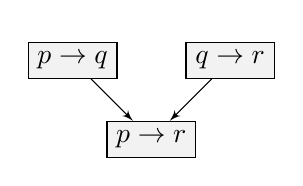
\begin{tikzpicture}
\node at (0,.3) {};
\node [block] (pimpliesq) at (-1,0) {$p \rightarrow q$};
\node [block] (p) at (1,0) {$q \rightarrow r$};
\node [block] (q) at (0,-1) {$p \rightarrow r$};
\path [line] (pimpliesq) -- (q);
\path [line] (p) -- (q);
\end{tikzpicture}
\end{center}
Each rule of inference will tell us how knowing certain propositions to be true leads us to learn other propositions are true. How do we read this rule of inference? If we know that \fbox{$p \rightarrow q$} is true and we know that \fbox{$q \rightarrow r$} is true, then we can conclude that \fbox{$p \rightarrow r$} is true.

Why should we accept this rule of inference? Consider the following truth table which presents the three propositions \fbox{$p \rightarrow q$} and  \fbox{$q \rightarrow r$} and \fbox{$p \rightarrow r$}.
\begin{center}
\begin{tabular}{c|c|c||c|c|c}
$p$ & $q$ & $r$ & $p \to q$ & $q \to r$ & $p \to r$ \\\hline
T & T & T & T& T & T \\
T & T & F & T& F& F\\
T & F & T & F& T& T \\
T & F & F & F& T& F\\
F & T & T & T& T& T\\
F & T & F & T& F& T\\
F & F & T & T& T & T\\
F & F & F & T & T& T
\end{tabular}
\end{center}
Although there are typically eight situations, let us remove any situations where $p \to q$ is false. We end up removing rows 3 and 4, resulting in
\begin{center}
\begin{tabular}{c|c|c||c|c|c}
$p$ & $q$ & $r$ & $p \to q$ & $q \to r$ & $p \to r$ \\\hline
T & T & T & T& T & T \\
T & T & F & T& F& F\\
F & T & T & T& T& T\\
F & T & F & T& F& T\\
F & F & T & T& T & T\\
F & F & F & T & T& T
\end{tabular}
\end{center}
We also only want to consider situations where $q \rightarrow r$ is true, so from the six rows above, let us remove the two rows where $q \to r$ is false. We are left with
\begin{center}
\begin{tabular}{c|c|c||c|c|c}
$p$ & $q$ & $r$ & $p \to q$ & $q \to r$ & $p \to r$ \\\hline
T & T & T & T& T & T \\
F & T & T & T& T& T\\
F & F & T & T& T & T\\
F & F & F & T & T& T
\end{tabular}
\end{center}
From our original $8$ rows, by removing any rows where $p \to q$ was false and also removing any rows where $q \to r$ is false, we are left with $4$ rows. In all four situations which remain, $p \to r$ is true. While we accept this rule of inference, we do not usually apply this rule of inference. (The typical rules of inference in a mathematician's toolbox start in Section~\ref{section:proving-using-conjunction}.)

Before jumping into that section, though, we present another (rare) rule of inference and argue why it should be trusted.
\begin{center}
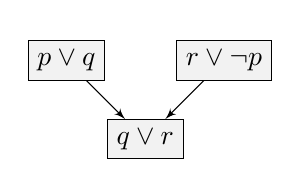
\begin{tikzpicture}
\node at (0,.3) {};
\node [block] (pimpliesq) at (-1,0) {$p \vee q$};
\node [block] (p) at (1,0) {$r \vee\neg p$};
\node [block] (q) at (0,-1) {$q \vee r$};
\path [line] (pimpliesq) -- (q);
\path [line] (p) -- (q);
\end{tikzpicture}
\end{center}
How do we read this? If we know \fbox{$p \vee q$} is true and we know \fbox{$r \vee\neg p$} is true, then we can conclude that \fbox{$q \vee r$} is true. Why do we trust this rule of inference? Why do we accept it? The truth table below presents \fbox{$p \vee q$} and  \fbox{$r \vee\neg p$} and \fbox{$q \vee r$}.
\begin{center}
\begin{tabular}{c|c|c||c|c|c}
$p$ & $q$ & $r$ & $p \vee q$ & $r \vee \neg p$ & $q \vee r$ \\\hline
T & T & T & T& T & T \\
T & T & F & T& F& T\\
T & F & T & T& T& T \\
T & F & F & T& F& F\\
F & T & T & T& T& T\\
F & T & F & T& T& T\\
F & F & T & F& T & T\\
F & F & F & F & T& F
\end{tabular}
\end{center}
Since we only want to consider situations where $p \vee q$ is true, let's remove rows where $p \vee q$ is false. We get:
\begin{center}
\begin{tabular}{c|c|c||c|c|c}
$p$ & $q$ & $r$ & $p \vee q$ & $r \vee \neg p$ & $q \vee r$ \\\hline
T & T & T & T& T & T \\
T & T & F & T& F& T\\
T & F & T & T& T& T \\
T & F & F & T& F& F\\
F & T & T & T& T& T\\
F & T & F & T& T& T
\end{tabular}
\end{center}
From these remaining $6$ rows, we only want to look at situations where $r \vee \neg p$ is true, so let's remove the rows where $r \vee \neg p$ is false:
\begin{center}
\begin{tabular}{c|c|c||c|c|c}
$p$ & $q$ & $r$ & $p \vee q$ & $r \vee \neg p$ & $q \vee r$ \\\hline
T & T & T & T& T & T \\
T & F & T & T& T& T \\
F & T & T & T& T& T\\
F & T & F & T& T& T
\end{tabular}
\end{center}
In all the rows that remain, the proposition $q \vee r$ is true. Thus, this rule of inference is valid. If $p \vee q$ is true and $r \vee \neg p$ is true, then it is automatically always the case that $q \vee r$ is true as well.

\begin{exercise}
Consider the following rule of inference:
\begin{center}
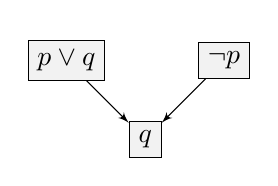
\begin{tikzpicture}
\node at (0,.3) {};
\node [block] (pimpliesq) at (-1,0) {$p \vee q$};
\node [block] (p) at (1,0) {$\neg p$};
\node [block] (q) at (0,-1) {$q$};
\path [line] (pimpliesq) -- (q);
\path [line] (p) -- (q);
\end{tikzpicture}
\end{center}
Answer the following questions:
\begin{enumerate}
\item What is this rule of inference stating?
\item Using a truth table (and removing rows from it), show that this rule of inference can be trusted as valid.
\end{enumerate}
\end{exercise}

\begin{exercise}
Consider the following rule of inference:
\begin{center}
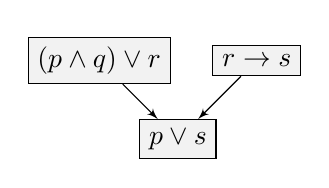
\begin{tikzpicture}
\node at (0,.3) {};
\node [block] (pimpliesq) at (-1,0) {$(p \wedge q) \vee r$};
\node [block] (p) at (1,0) {$r \to s$};
\node [block] (q) at (0,-1) {$p \vee s$};
\path [line] (pimpliesq) -- (q);
\path [line] (p) -- (q);
\end{tikzpicture}
\end{center}
Answer the following questions:
\begin{enumerate}
\item What is this rule of inference stating?
\item Using a truth table (and removing rows from it), show that this rule of inference can be trusted as valid.
\end{enumerate}
\end{exercise}

\subsection{Proving/using conjunctions}\label{section:proving-using-conjunction}

We use the proposition $p \wedge q$ according to the following flowchart:
\begin{bmethod}{Using a conjunction}{using-conjunction}
%Suppose $p \wedge q$ is known to be true. Then you can conclude $p$ is true. You can also conclude $q$ is true.
\begin{center}
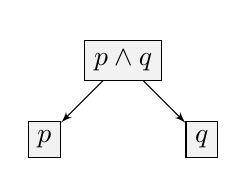
\begin{tikzpicture}
\node at (0,.3) {};
\node [block] (p-and-q) at (0,0) {$p \wedge q$};
\node [block] (p) at (-1,-1) {$p$};
\node [block] (q) at (1,-1) {$q$};
\path [line] (p-and-q) -- (p);
\path [line] (p-and-q) -- (q);
\end{tikzpicture}
\end{center}
\end{bmethod}
Visually, we have written $p \wedge q$ at the top, and have an arrow down to $p$ as well as an arrow down to $q$. Suppose that $p \wedge q$ is already established to be true (whether we were told to assume it in the beginning, or through the course of writing a proof, we discovered this fact to be true). How can we use $p \wedge q$? We can conclude that $p$ is true. We can also conclude that $q$ is true.

Why should we accept this rule of inference? This rule of inference is based on the definition of conjunction. Take the truth table of conjunction, and note that there are three rows where $p \wedge q$ is false. If we remove these three rows, we are left with
\begin{center}
\begin{tabular}{c|c||c}
$p$ & $q$ & $p \wedge q$ \\\hline
$T$ & $T$ & $T$
\end{tabular}
\end{center}
and notice that $p$ is true, and also that $q$ is true. Think of the flowchart above as a small puzzle piece used in a larger puzzle.
\begin{example}
Suppose we knew ``$c$ is a snark and $d$ eats vegetables.'' Then we can conclude ``$c$ is a snark.'' We can also conclude ``$d$ eats vegetables.''
\end{example}
\begin{example}
Suppose we knew (or were told, or just proved) that ``$a$ is even and $b$ is even.'' Then we can conclude that ``$a$ is even.'' We can also conclude that ``$b$ is even.''
\end{example}
\begin{example}\label{example:a-odd-and-b-odd-use-and}
Suppose we knew (or were told, or just proved) that ``$a$ is odd and $b$ is odd.'' Then we can conclude that ``$a$ is odd.'' We can also conclude that ``$b$ is odd.''
\end{example}

The puzzle piece we saw has $p \wedge q$ at the top, and we saw what facts can be obtained from having $p \wedge q$ be true. Another ``puzzle piece'' is the flowchart for \emph{proving} the proposition $p \wedge q$. Notice that in this flowchart, $p \wedge q$ is at the bottom:
\begin{bmethod}{Proving a conjunction}{proving-conjunction}
\begin{center}
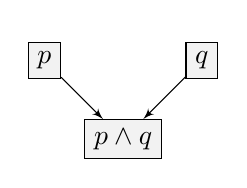
\begin{tikzpicture}
\node at (0,.3) {};
\node [block] (p) at (-1,0) {$p$};
\node [block] (q) at (1,0) {$q$};
\node [block] (p-and-q) at (0,-1) {$p \wedge q$};
\path [line] (p) -- (p-and-q);
\path [line] (q) -- (p-and-q);
\end{tikzpicture}
\end{center}
\end{bmethod}
How should we read this? As soon as $p$ is established to be true and $q$ is also established to be true, we can then conclude that $p \wedge q$ is true. Why should we accept this rule of inference? Start with the truth table for conjunction and remove any rows where there is an $F$ in the column for $p$, since we are in the situation where $p$ is true. Similarly, because $q$ is true, remove any rows where there is an $F$ for the $q$ column. In all remaining rows, the column for $p \wedge q$ always has a $T$.
\begin{example}
Suppose we were told to assume that ``$s$ has a dog.'' Suppose we were also told to assume that ``$t$ has a cat.'' Then we can conclude that ``$s$ has a dog and $t$ has a cat.''
\end{example}

\subsection{Proving/using implications}\label{section:proving-using-implication}

There are two main ways to use the implication $p \rightarrow q$. The first method of using $p \rightarrow q$ is called \defn{modus ponens}\index{modus ponens}:
\begin{bmethod}{Using an implication (modus ponens)}{modus-ponens}
\begin{center}
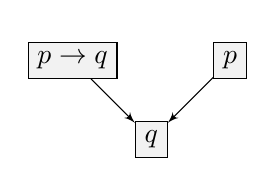
\begin{tikzpicture}
\node at (0,.3) {};
\node [block] (pimpliesq) at (-1,0) {$p \rightarrow q$};
\node [block] (p) at (1,0) {$p$};
\node [block] (q) at (0,-1) {$q$};
\path [line] (pimpliesq) -- (q);
\path [line] (p) -- (q);
\end{tikzpicture}
\end{center}
\end{bmethod}
Modus ponens is saying that, in the course of a proof, if you know that $p \rightarrow q$ is true and you know that $p$ is true, then you can conclude that $q$ is true. Why should we accept modus ponens as one of our rules of inference? Start with the truth table for implication:
\begin{center}
\begin{tabular}{c|c||c}
$p$ & $q$ & $p \rightarrow q$ \\\hline
$T$ & $T$ & $T$\\
$T$ & $F$ & $F$\\
$F$ & $T$ & $T$\\
$F$ & $F$ & $T$
\end{tabular}
\end{center}
Since we are in the situation where $p \rightarrow q$ is true, let us remove the one situation where $p \rightarrow q$ is false. So we have
\begin{center}
\begin{tabular}{c|c||c}
$p$ & $q$ & $p \rightarrow q$ \\\hline
$T$ & $T$ & $T$\\
$F$ & $T$ & $T$\\
$F$ & $F$ & $T$
\end{tabular}
\end{center}
We are also in the situation where $p$ is already true, so of the three remaining situations, let us remove the rows where $p$ is false. We are left with
\begin{center}
\begin{tabular}{c|c||c}
$p$ & $q$ & $p \rightarrow q$ \\\hline
$T$ & $T$ & $T$\\
\end{tabular}
\end{center}
and $q$ must therefore be true.
\begin{example}
Suppose we were allowed to assume ``If $x$ is a borogove, then $x$ is a tove'' and we were also instructed to assume that ``$x$ is a borogove'' is true. Then, we can conclude ``$x$ is a tove'' via modus ponens.
\end{example}
\begin{example}
Suppose we had just proved the implication ``If $s^2$ is even, then $s$ is even'' and we were instructed to assume that ``$s^2$ is even'' is true. Then, we can conclude ``$s$ is even'' via modus ponens.
\end{example}

Another way to use the implication $p \rightarrow q$ is \defn{modus tollens}\index{modus tollens}:
\begin{bmethod}{Using an implication (modus tollens)}{modus-tollens}
\begin{center}
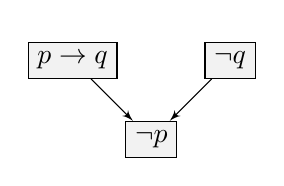
\begin{tikzpicture}
\node at (0,.3) {};
\node [block] (pimpliesq) at (-1,0) {$p \rightarrow q$};
\node [block] (negq) at (1,0) {$\neg q$};
\node [block] (negp) at (0,-1) {$\neg p$};
\path [line] (pimpliesq) -- (negp);
\path [line] (negq) -- (negp);
\end{tikzpicture}
\end{center}
\end{bmethod}
You should convince yourself that it is reasonable to accept modus tollens as a rule of inference: start with the truth table for $p \rightarrow q$. Remove any rows where $p \rightarrow q$ is false. Remove any rows where $\neg q$ is false. In all remaining rows, note that $\neg p$ is true.
\begin{example}
Suppose we were allowed to assume ``If $x$ is a borogove, then $x$ is a tove'' and we were also instructed to assume that ``$x$ is not a tove'' is true. Then, we can conclude ``$x$ is not a borogove'' via modus tollens.
\end{example}
\begin{example}
Suppose we had just proved the implication ``If $s^2$ is even, then $s$ is even'' and we were instructed to assume that ``$s^2$ is not even'' is true. Then, we can conclude ``$s$ is not even'' via modus tollens.
\end{example}
\begin{bwarning}{}{}
It is not possible to conclude anything from the propositions $p \rightarrow q$ and $q$, though someone new to proof is often tempted to conclude $p$. In other words, following the flowchart
\begin{center}
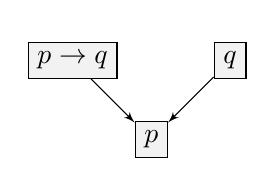
\begin{tikzpicture}
\node at (0,.3) {};
\node [block] (pimpliesq) at (-1,0) {$p \rightarrow q$};
\node [block] (negq) at (1,0) {$q$};
\node [block] (negp) at (0,-1) {$p$};
\path [line] (pimpliesq) -- (negp);
\path [line] (negq) -- (negp);
\end{tikzpicture}
\end{center}
is not valid reasoning.
\end{bwarning}
\begin{example}
Suppose we were allowed to assume ``If $x$ is a borogove, then $x$ is a tove'' and we were also instructed to assume that ``$x$ is a tove'' is true. 
That we cannot conclude anything, because neither modus ponens nor modus tollens will apply. In particular, we do not obtain ``$x$ is a borogove'' as a conclusion.
\end{example}

There are several ways to prove the implication $p \rightarrow q$. We introduce the \defn{direct proof}\index{direct proof} of $p \rightarrow q$ here, and save the other methods for Sections~\ref{section:indirect-proof} and~\ref{section:proof-by-contradiction}:
\begin{bmethod}{Proving an implication (direct proof)}{proving-implication-direct}
\begin{center}
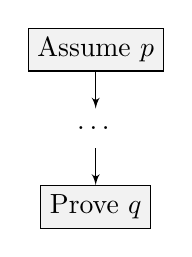
\begin{tikzpicture}
\node [block] (assume-p) at (0,0) {Assume $p$};
\path [line] (assume-p) -- (0,-.75);
\node at (0,-1) {$\dots$};
\node [block] (q) at (0,-2) {Prove $q$};
\path [line] (0,-1.25) -- (q);
\end{tikzpicture}
\end{center}
\end{bmethod}
We will use the direct proof so often, let us highlight this strategy:
\begin{bmethod}{Direct proof of $p \rightarrow q$}{direct-proof-method}
To prove the implication $p \rightarrow q$, assume that $p$ is true. Then use rules of inference to (eventually) obtain the fact that $q$ is true.
\end{bmethod}
\begin{example}
Consider the implication ``If Jo buys a car, then Jo lives in an apartment.'' To prove this proposition via the direct proof method, the author of the proof would start by writing ``Assume that Jo buys a car.'' The goal is to then prove that ``Jo lives in an apartment.''
\end{example}
The word ``assume'' and the word ``suppose'' used to start a sentence in a proof have the same role. Here is an example.
\begin{example}\label{example:aoddandbodd-implies-aplusbeven-directproof}
Consider the implication ``If $a$ is odd and $b$ is odd, then $a+b$ is even.'' To prove this implication via the direct proof method, the first sentence of the proof should be ``Suppose $a$ is odd and $b$ is odd.'' The goal in the remainder of the proof is to obtain the proposition ``$a+b$ is even.'' To get to that point, there will be many other sentences which advance the logic forward, so the writer of the proof might indicate this eventual goal by writing ``We want to show that $a+b$ is even.''
\end{example}

\subsection{Proving/using existentially-quantified statements}\label{section:proving-using-existential}

To use the existentially-quantified statement $\exists x \in U\,[P(x)]$, we introduce a new rule of inference:
\begin{bmethod}{Using an existentially-quantified statement}{using-exists}
\begin{center}
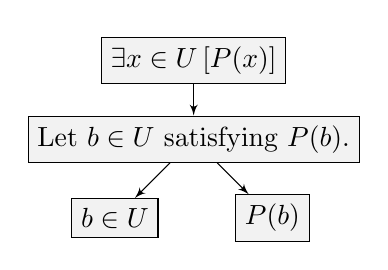
\begin{tikzpicture}
\node at (0,1.3) {};
\node [block] (exists) at (0,1) {$\exists x \in U\,[P(x)]$};
\node [block] (p-and-q) at (0,0) {Let $b \in U$ satisfying $P(b)$.};
\node [block] (p) at (-1,-1) {$b \in U$};
\node [block] (q) at (1,-1) {$P(b)$};
\path [line] (exists) -- (p-and-q);
\path [line] (p-and-q) -- (p);
\path [line] (p-and-q) -- (q);
\end{tikzpicture}
\end{center}
\end{bmethod}
If we are to start with $\exists x \in U\,[P(x)]$ being true, since there exists something in $U$, and if that something were called $x$, then $P(x)$ is true, we should make such an object. In the flowchart above, we intentionally use a new variable $b$. It may be the case that you have already used $b$ in your proof. Then, use another letter. The word ``Let'' should always be followed by a new variable that has not yet been used. For example, the sentence \fbox{Let $b \in U$ satisfying $P(b)$.} written in a proof creates a new object called $b$, and $b$ happens to be a member of $U$ and, in addition, $P(b)$ is true. We can make such an object (called $b$) because it was previously established that there exists $x \in U$ such that $P(x)$.

\begin{example}
Say we know \fbox{$\exists m \in Y [P(m)]$} is true. Then, as long as $b$ has not been written in our proof yet, we could write \fbox{Let $b \in Y$ satisfying $P(b)$}, then from this conclude that \fbox{$b \in Y$} and \fbox{$P(b)$} are true.
\end{example}
\begin{example}
Say we know \fbox{there exists $h \in L$ such that $P(h)$} is true. Then, as long as $b$ has not been written in our proof yet, we could write \fbox{Let $b \in L$ satisfying $P(b)$}, then from this conclude that \fbox{$b \in L$} and \fbox{$P(b)$} are true.
\end{example}
\begin{example}
Say we know \fbox{there exists $m \in S$ such that $P(m)$} is true. Then, as long as $y$ has not been written in our proof yet, we could write \fbox{Let $y \in S$ satisfying $P(y)$}, then from this conclude that \fbox{$y \in S$} and \fbox{$P(y)$} are true.
\end{example}
\begin{example}
Say we knew that \fbox{there exists $c \in D$ such that $c$ plays soccer} is true. Then, as long as $b$ has not been written in our proof yet, we could use this by writing \fbox{Let $b \in D$ satisfying $b$ plays soccer}, then conclude from this that \fbox{$b \in D$} and \fbox{$b$ plays soccer} are true.
\end{example}
\begin{example}
Say we knew that \fbox{there exists $c \in D$ such that $c$ plays soccer} is true. Then, if $b$ has been used in our proof, but $k$ has not, we could use this by writing \fbox{Let $k \in D$ satisfying $k$ plays soccer}, then conclude from this that \fbox{$k \in D$} and \fbox{$k$ plays soccer} are true.
\end{example}

\begin{example}
Suppose we were told to assume the proposition ``There exists an $x \in \mathbb{H}$ such that $x$ has dual citizenship.'' To use this proposition, we would include in our proof the sentence ``Let $b$ be in $\mathbb{H}$ satisfying the property that $b$ has dual citizenship.'' Then, we could draw two additional conclusions. We can conclude $b \in \mathbb{H}$. We can also conclude $b$ has dual citizenship.
\end{example}
\begin{example}\label{example:use-existence-revisit-first-proof}
Suppose we were to assume ``There exists $k \in \mathbb{Z}$ such that $a=2k+1$.'' Then, we could write ``Let $x \in \mathbb{Z}$ satisfying $a=2x+1$.'' 
From here, we could conclude $x \in \mathbb{Z}$. We could also conclude $a=2x+1$.
\end{example}

To prove the existentially-quantified statement $\exists x \in U\,[P(x)]$, follow the flowchart:
\begin{bmethod}{Proving an existentially-quantified statement}{proving-exists}
\begin{center}
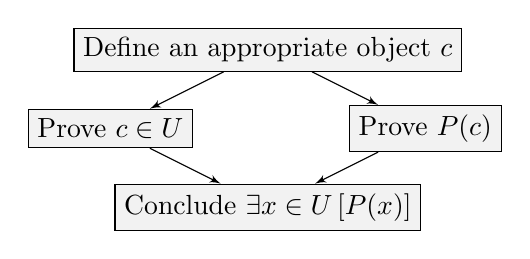
\begin{tikzpicture}
\node [block] (exists) at (0,1) {Define an appropriate object $c$};
\node [block] (p) at (-2,0) {Prove $c \in U$};
\node [block] (q) at (2,0) {Prove $P(c)$};
\node [block] (p-and-q) at (0,-1) {Conclude $\exists x \in U\,[P(x)]$};
\path [line] (exists) -- (p);
\path [line] (exists) -- (q);
\path [line] (p) -- (p-and-q);
\path [line] (q) -- (p-and-q);
\end{tikzpicture}
\end{center}
\end{bmethod}

It is extremely intentional that $c$ is used in three locations. First, $c$ should be defined. Then, using how $c$ was defined, prove that $c \in U$. Third, using the $c$ that was defined, prove $P(c)$. The emphasis is that it must be the same $c$. In other words, both $c \in U$ and $P(c)$ must simultaneously be true. This is the only way we could rightly conclude that there exists an $x \in U$ such that $P(x)$ is true.

\begin{bremark}{Proving something exists}{proving-existence}
This is essentially a restating of the flowchart above. To prove that something exists and satisfies a certain property, make an object (say we call it $c$) and prove that all the necessary properties are true for that object: in this case, prove that $c \in U$ and prove that $P(c)$ is true. In short, to convince someone that a certain thing exists, make the thing! To prove $\exists m \in U$ such that $P(m)$ is true, you should find an object $c$ in $U$ be carefully defining $c$, then show $P(c)$.
\vskip6pt
In order to prove something exists (and has a certain behavior), you should find it (and show that it has that behavior).
\end{bremark}





\begin{example}
Say we need to prove \fbox{$\exists m \in Y [P(m)]$} is true. Then, as long as $b$ has not been written in our proof yet, we could define $b$. Then, with this $b$, prove that \fbox{$b \in Y$} and \fbox{$P(b)$} are true.
\end{example}
\begin{example}
Say we need to prove \fbox{there exists $h \in L$ such that $P(h)$} is true. Then, as long as $b$ has not been written in our proof yet, define $b$. Then, based on what you have said $b$ is, prove that \fbox{$b \in L$} and \fbox{$P(b)$} are true.
\end{example}
\begin{example}
Say we need to prove \fbox{there exists $m \in S$ such that $P(m)$} is true. Then, as long as $y$ has not been written in our proof yet, define $y$. Then, based on how you defined $y$, prove \fbox{$y \in S$} and also prove \fbox{$P(y)$}.
\end{example}
\begin{example}
Say we need to prove \fbox{there exists $c \in D$ such that $c$ plays soccer} is true. Then, as long as $b$ has not been written in our proof yet, define something to be $b$. If $b$ has been defined appropriately, then it will be possible to prove \fbox{$b \in D$} and \fbox{$b$ plays soccer} are true.
\end{example}
\begin{example}
Say we need to prove \fbox{there exists $c \in D$ such that $c$ plays soccer} is true. Then, if $b$ has been used in our proof, but $k$ has not, carefully define $k$, and based on how you defined $k$, prove \fbox{$k \in D$} and \fbox{$k$ plays soccer} are true.
\end{example}


\begin{example}\label{example:prove-existence-revisit-first-proof}
Suppose we have the task of needing to prove $\exists k \in \mathbb{Z}\,[a+b=2k]$. If so, we should define $z$. Then, based on how we have defined $z$, we would need to prove $z \in \mathbb{Z}$. We also would need to prove $a+b=2z$. If we are successful proving both of these things, we would then be able to conclude $\exists k \in \mathbb{Z}\,[a+b=2k]$.
\end{example}

As another example, let us consider the proof of this short theorem.
\begin{theorem}\label{theorem:existence-not-uniqueness}
There exists a real number $b$ such that $b^2-3b=40$.
\end{theorem}
\begin{proof}
Let $b = 8$. Then $b \in \mathbb{R}$. Also, $b^2-3b=8^2-3(8)=40$.
\end{proof}
Of course, this is not the only possible proof of this theorem. Here is another proof:
\begin{proof}
Let $a = 8$. Then $a \in \mathbb{R}$. Also, $a^2-3a=(-5)^2-3(-5)=40$.
\end{proof}

\begin{exercise}
Using the hypotheses
\begin{itemize}
\item If it does not rain or if it is not foggy, then the sailing race will be held and the lifesaving demonstration will go on.
\item If the sailing race is held, then the trophy will be awarded.
\item The trophy was not awarded.
\end{itemize}
prove (in full sentences) the statement ``It rained.''
\quad\quad\href{https://www.sharelatex.com/project/59ceb65136e6671a14199aec}{{\color{red}[key]}}
\end{exercise}

\subsection{Proving/using a fact by definition}\label{section:proving-using-definition}

Suppose we had a predicate $P(z)$, and using this predicate, suppose that a definition had previously been established that said \fbox{Definition: We say $z$ is a \defn{borogove} if $P(z)$.}

We introduce flowcharts for proving $g$ is a borogove and -- just to use a different letter -- using the fact that $m$ is a borogove. %Keep this order: proving first, then using, due to the structure of this sentence.
\begin{bmethod}{Proving $g$ is a borogove}{proving-borogove}
\begin{center}
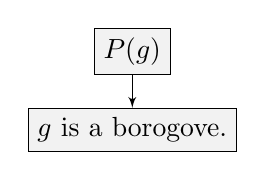
\begin{tikzpicture}
\node [block] (upper) at (0,0) {$P(g)$};
\node [block] (lower) at (0,-1) {$g$ is a borogove.};
\path [line] (upper) -- (lower);
\end{tikzpicture}
\end{center}
\end{bmethod}
\begin{bmethod}{Using $m$ is a borogove}{using-borogove}
\begin{center}
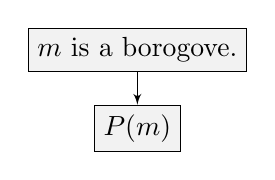
\begin{tikzpicture}
\node [block] (upper) at (0,0) {$m$ is a borogove.};
\node [block] (lower) at (0,-1) {$P(m)$};
\path [line] (upper) -- (lower);
\end{tikzpicture}
\end{center}
\end{bmethod}

\begin{blanguage}{Every definition behaves like an ``if and only if'' statement}{definition-iff}
By staring at the rules of inference for using and proving a definition, you may notice that we are using the text \fbox{$z$ is a \defn{borogove} if $P(z)$} as if it says \fbox{$z$ is a \defn{borogove} if and only if $P(z)$}. While there are some authors that insist on writing the phrase ``if and only if'' in each definition for this very reason, the majority of authors only use the word ``if.'' Nevertheless, when reading definitions from these authors, one use of the word ``if'' in the definition truly operates as an ``if and only if.''
\end{blanguage}
This handbook on proof follows the convention that the majority of mathematical authors use: one use of the word `if' in each definition operates as an `if and only if,' but the word `if' is used nonetheless.

While you are certainly familiar with integers that are even and integers that are odd, to manipulate odd and even numbers in proofs, we will need definitions:
\begin{bdefinition}{Even}{even}
The integer $n$ is \defn{even}\index{even} if there exists an integer $k$ such that $n=2k$.
\end{bdefinition}
\begin{bdefinition}{Odd}{odd}
The integer $n$ is \defn{odd}\index{odd} if there exists an integer $k$ such that $n=2k+1$.
\end{bdefinition}
Be referencing the definition of odd, here are flowcharts (based on the template flowcharts in Methods~\ref{method:proving-borogove} and~\ref{method:using-borogove}) for using $a$ is odd and for proving $c$ is odd:
\begin{center}
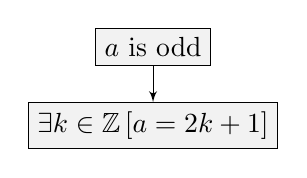
\begin{tikzpicture}
\node [block] (upper) at (0,0) {$a$ is odd};
\node [block] (lower) at (0,-1) {$\exists k \in \mathbb{Z}\,[a=2k+1]$};
\path [line] (upper) -- (lower);
\end{tikzpicture}
\quad
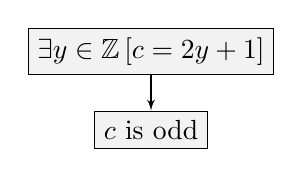
\begin{tikzpicture}
\node [block] (upper) at (0,0) {$\exists y \in \mathbb{Z}\,[c=2y+1]$};
\node [block] (lower) at (0,-1) {$c$ is odd};
\path [line] (upper) -- (lower);
\end{tikzpicture}
\end{center}
\begin{exercise}
Write for yourself flowcharts for using $r$ is even and for proving $s$ is even.
\end{exercise}

\begin{exercise}
In Exercise~\ref{exercise:disjunction-checklist}, you were asked to consider what are things that must be addressed in writing a definition of disjunction. Similarly, what are things that you must address when writing a definition for odd?
\end{exercise}
\begin{exercise}
In Exercise~\ref{exercise:disjunction-checklist}, you were asked to consider what are things that must be addressed in writing a definition of disjunction. Similarly, what are things that you must address when writing a definition for even?
\end{exercise}

\begin{example}
Consider the following definition: A real number $m$ is \defn{duporous} if there exists an integer $c$ such that $m=2^c$.

If we were given the fact that \fbox{$r$ is duporous} is true, then we can conclude that there exists an integer $d$ such that $r=2^d$. This follows Method~\ref{method:using-borogove}.

On the other hand, suppose we needed to prove that $y$ is duporous. (For the sake of simplicity, suppose we already knew that $y$ is real.) Then, we should first prove the statement ``there exists an integer $k$ such that $y=2^k$.'' After proving this, we could conclude that $y$ is duporous.  This follows Method~\ref{method:proving-borogove}.
\end{example}
Notice in this example that the text of the definition of dupourous only has the word ``if'' instead of the phrase ``if and only if.'' However, we operate as if the sentence were ``A real number $m$ is \defn{duporous} if and only if there exists an integer $c$ such that $m=2^c$.'' See Language Discussion~\ref{language:definition-iff}.

\begin{bwarning}{}{}
It is tempting to ignore these two definitions. Don't. Notice that both definitions above include the phrase ``there exists.'' We will need to deal with the phrase ``there exists'' in the manner introduced in Section~\ref{section:proving-using-existential}. It will be impossible to do proofs if you think of ``$n$ is even'' as being ``$n$ can be divided by $2$ with no remainder'' or similar notions such as ``$2$ goes evenly into $n$.'' These phrases are unhelpful for proof (because we have no rules of inference that deals with the phrase ``goes evenly into.''
\end{bwarning}

We are now ready to prove our first theorem:
\begin{theorem}\label{theorem:odd-plus-odd-is-even}
If $a$ is odd and $b$ is odd, then $a+b$ is even.
\end{theorem}
Your intuition might tell you this statement is ``true.'' After all, $3+5=8$ and $11+9=20$. However, thinking of a million examples where this seems to be true does not make a proof! Examples are helpful as intuition, but they are not substitutes for the proof.

The first several times you work on a proof, it will seem like an immense amount of work. It will be tempting to think, ``Why should I follow such dry methods of proof when I can use my intuition on this statement?'' In future math classes, you will be expected to prove statements for which you will have no intuition at all. However, the methods of proof will apply. Even if the theorem above seems silly, this is a chance to practice the methods of proof.

Notice that Theorem~\ref{theorem:odd-plus-odd-is-even} is an implication. To prove an implication, we follow Method~\ref{method:direct-proof-method}, so we will assume that \fbox{$a$ is odd and $b$ is odd} and work to prove \fbox{$a+b$ is even}. (See Example~\ref{example:aoddandbodd-implies-aplusbeven-directproof}.) If we were to organize this in a flowchart, the flowchart of logic so far would look like this:
\begin{center}
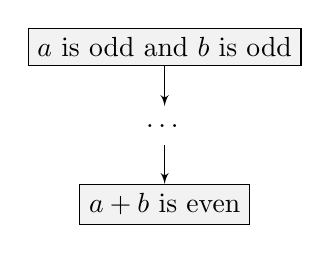
\begin{tikzpicture}
\node [block] (assume-p) at (0,0) {$a$ is odd and $b$ is odd};
\path [line] (assume-p) -- (0,-.75);
\node at (0,-1) {$\dots$};
\node [block] (q) at (0,-2) {$a+b$ is even};
\path [line] (0,-1.25) -- (q);
\end{tikzpicture}
\end{center}
We need to use the rules of inference to connect these two propositions. (This is what the dots represent -- details which we need to fill in.) The statement \fbox{$a$ is odd and $b$ is odd} is a conjunction, and since we are assuming this to be true, let's use this statement, following Method~\ref{method:using-conjunction}. (In fact, we have already done this work in Example~\ref{example:a-odd-and-b-odd-use-and}.) Now our flowchart is
\begin{center}
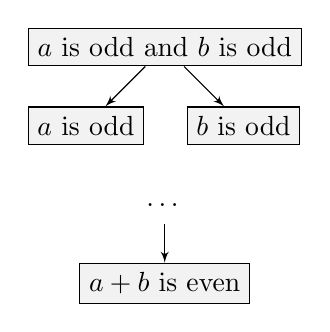
\begin{tikzpicture}
\node [block] (assume-p) at (0,0) {$a$ is odd and $b$ is odd};
\node [block] (a-odd) at (-1,-1) {$a$ is odd};
\node [block] (b-odd) at (1,-1) {$b$ is odd};
\path [line] (assume-p) -- (a-odd);
\path [line] (assume-p) -- (b-odd);
\node at (0,-2) {$\dots$};
\node [block] (q) at (0,-3) {$a+b$ is even};
\path [line] (0,-2.25) -- (q);
\end{tikzpicture}
\end{center}
We should use the fact that $a$ is odd, a flowchart which we already wrote out and can borrow. We similarly use the fact that $b$ is odd, also modeled after Method~\ref{method:using-borogove}. With these additions, our flowchart is now:
\begin{center}
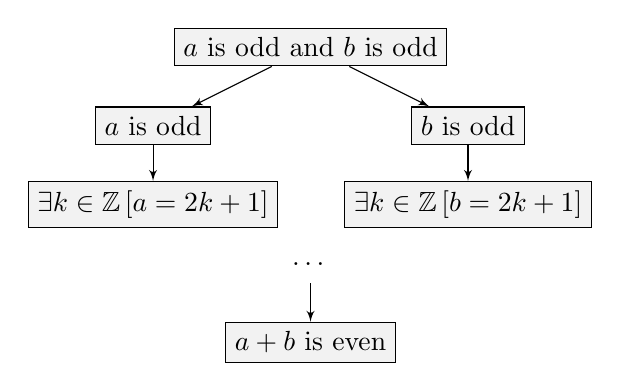
\begin{tikzpicture}
\node [block] (assume-p) at (0,0) {$a$ is odd and $b$ is odd};
\node [block] (a-odd) at (-2,-1) {$a$ is odd};
\node [block] (b-odd) at (2,-1) {$b$ is odd};
\path [line] (assume-p) -- (a-odd);
\path [line] (assume-p) -- (b-odd);
\node [block] (a-odd-use) at (-2,-2) {$\exists k \in \mathbb{Z}\,[a=2k+1]$};
\node [block] (b-odd-use) at (2,-2) {$\exists k \in \mathbb{Z}\,[b=2k+1]$};
\path [line] (a-odd) -- (a-odd-use);
\path [line] (b-odd) -- (b-odd-use);
\node at (0,-2.75) {$\dots$};
\node [block] (q) at (0,-3.75) {$a+b$ is even};
\path [line] (0,-3) -- (q);
\end{tikzpicture}
\end{center}
It is helpful to work on the lower portion of the flowchart. What is it going to take for $a+b$ to be even? (In other words, what will need to be the box immediately before?) Here, Method~\ref{method:proving-borogove} applies and our updated flowchart is:
\begin{center}
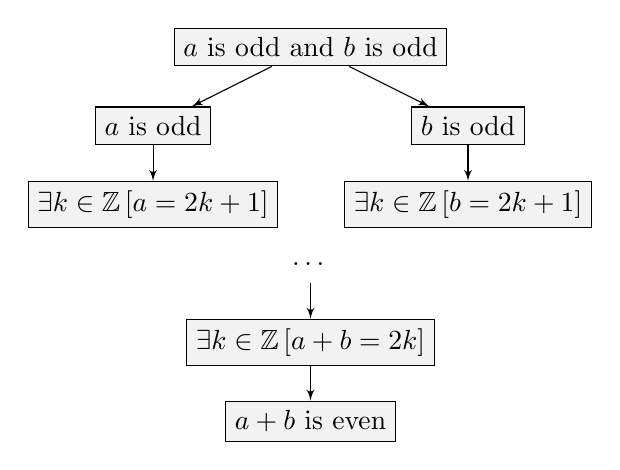
\begin{tikzpicture}
\node [block] (assume-p) at (0,0) {$a$ is odd and $b$ is odd};
\node [block] (a-odd) at (-2,-1) {$a$ is odd};
\node [block] (b-odd) at (2,-1) {$b$ is odd};
\path [line] (assume-p) -- (a-odd);
\path [line] (assume-p) -- (b-odd);
\node [block] (a-odd-use) at (-2,-2) {$\exists k \in \mathbb{Z}\,[a=2k+1]$};
\node [block] (b-odd-use) at (2,-2) {$\exists k \in \mathbb{Z}\,[b=2k+1]$};
\path [line] (a-odd) -- (a-odd-use);
\path [line] (b-odd) -- (b-odd-use);
\node at (0,-2.75) {$\dots$};
\node [block] (def-even) at (0,-3.75) {$\exists k \in \mathbb{Z}\,[a+b=2k]$};
\node [block] (q) at (0,-4.75) {$a+b$ is even};
\path [line] (0,-3) -- (def-even);
\path [line] (def-even) -- (q);
\end{tikzpicture}
\end{center}
We have two existence statements which we have not yet used. We update the flowchart, informed by Method~\ref{method:using-exists}, keeping in mind that each ``Let'' sentence should use a \emph{new} variable. (See our work in Example~\ref{example:use-existence-revisit-first-proof}.)
\begin{center}
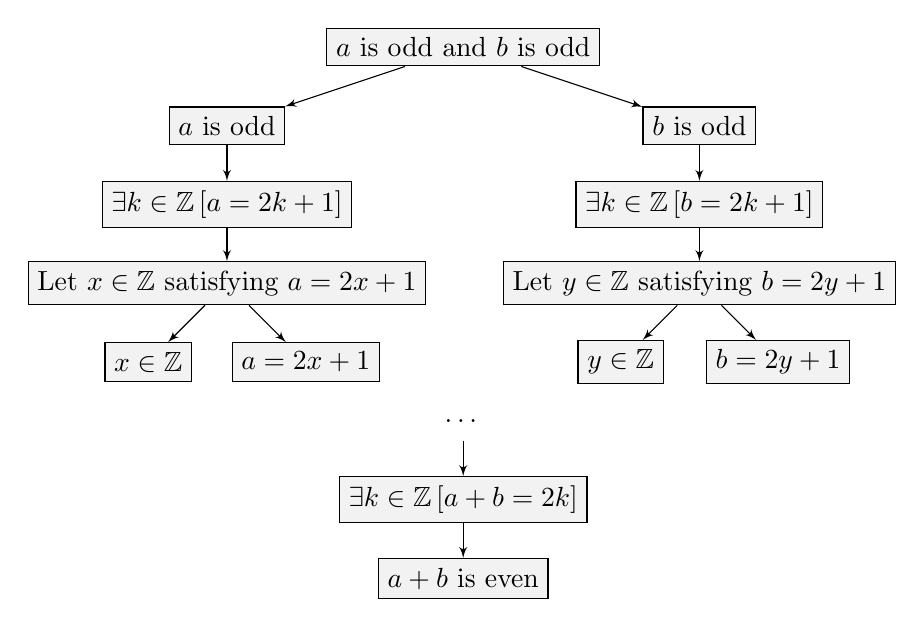
\begin{tikzpicture}
\node [block] (assume-p) at (0,0) {$a$ is odd and $b$ is odd};
\node [block] (a-odd) at (-3,-1) {$a$ is odd};
\node [block] (b-odd) at (3,-1) {$b$ is odd};
\path [line] (assume-p) -- (a-odd);
\path [line] (assume-p) -- (b-odd);
\node [block] (a-odd-use) at (-3,-2) {$\exists k \in \mathbb{Z}\,[a=2k+1]$};
\node [block] (b-odd-use) at (3,-2) {$\exists k \in \mathbb{Z}\,[b=2k+1]$};
\path [line] (a-odd) -- (a-odd-use);
\path [line] (b-odd) -- (b-odd-use);
\node [block] (a-exist-use) at (-3,-3) {Let $x \in \mathbb{Z}$ satisfying $a=2x+1$};
\node [block] (b-exist-use) at (3,-3) {Let $y \in \mathbb{Z}$ satisfying $b=2y+1$};
\path [line] (a-odd-use) -- (a-exist-use);
\path [line] (b-odd-use) -- (b-exist-use);
\node [block] (x-int) at (-4,-4) {$x \in \mathbb{Z}$};
\node [block] (ax-eq) at (-2,-4) {$a=2x+1$};
\path [line] (a-exist-use) -- (x-int);
\path [line] (a-exist-use) -- (ax-eq);
\node [block] (y-int) at (2,-4) {$y \in \mathbb{Z}$};
\node [block] (by-eq) at (4,-4) {$b=2y+1$};
\path [line] (b-exist-use) -- (y-int);
\path [line] (b-exist-use) -- (by-eq);
\node at (0,-4.75) {$\dots$};
\node [block] (def-even) at (0,-5.75) {$\exists k \in \mathbb{Z}\,[a+b=2k]$};
\node [block] (q) at (0,-6.75) {$a+b$ is even};
\path [line] (0,-5) -- (def-even);
\path [line] (def-even) -- (q);
\end{tikzpicture}
\end{center}
We have already done a lot of work, and this may seem overwhelming at first, but this process will get easier. Up to this point, everything (other than choosing to use the letters $x$ and $y$) done was very methodical and did not require creativity. We now enter the creative phase of this proof. We still need to prove \fbox{$\exists k \in \mathbb{Z}\,[a+b=2k]$} and to prove this statement, Method~\ref{method:proving-exists} says we need to define an appropriate object. Let's say that the object we define will be called $z$, though we could have used any letter other than $x$, $y$, $a$, or $b$. (See Example~\ref{example:prove-existence-revisit-first-proof}.) Not \emph{only} do we have to define $z$, but $z$ needs to be defined in such a way that two things are true. First, we will need $z \in \mathbb{Z}$ and second, we will need $a+b=2z$. Note that we are allowed to use the facts that $a=2x+1$ and $b=2y+1$. In fact, we should define $z$ in \emph{in terms of} these already-defined variables $x$, $y$, $a$, and $b$.

If we consider $a+b$, we can rewrite this as $a+b=(2x+1)+(2y+1)$ and using further properties of algebra, this can be rewritten as $2x+2y+1+1=2x+2y+2=2(x+y+1)$. In short, using the facts $a=2x+1$ and $b=2y+1$, we see that $a+b=2(x+y+1)$, yet recall we need to define an integer $z$ such that $a+b=2z$. It seems we should define $z$ to be $x+y+1$. In fact, note that because $x$ and $y$ are integers, $z$ is an integer (since the sum of integers is an integer, the closure of addition stated in Section~\ref{section:examples-of-assumed-propositions}). This will complete the flowchart:
\begin{center}
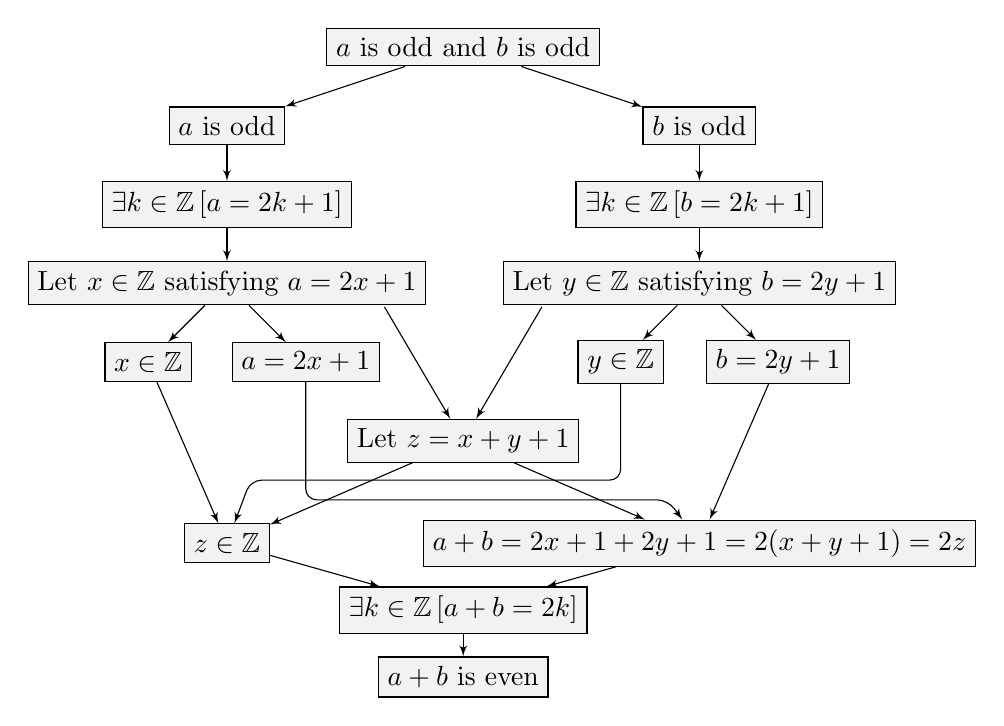
\begin{tikzpicture}
\node [block] (assume-p) at (0,0) {$a$ is odd and $b$ is odd};
\node [block] (a-odd) at (-3,-1) {$a$ is odd};
\node [block] (b-odd) at (3,-1) {$b$ is odd};
\path [line] (assume-p) -- (a-odd);
\path [line] (assume-p) -- (b-odd);
\node [block] (a-odd-use) at (-3,-2) {$\exists k \in \mathbb{Z}\,[a=2k+1]$};
\node [block] (b-odd-use) at (3,-2) {$\exists k \in \mathbb{Z}\,[b=2k+1]$};
\path [line] (a-odd) -- (a-odd-use);
\path [line] (b-odd) -- (b-odd-use);
\node [block] (a-exist-use) at (-3,-3) {Let $x \in \mathbb{Z}$ satisfying $a=2x+1$};
\node [block] (b-exist-use) at (3,-3) {Let $y \in \mathbb{Z}$ satisfying $b=2y+1$};
\path [line] (a-odd-use) -- (a-exist-use);
\path [line] (b-odd-use) -- (b-exist-use);
\node [block] (x-int) at (-4,-4) {$x \in \mathbb{Z}$};
\node [block] (ax-eq) at (-2,-4) {$a=2x+1$};
\path [line] (a-exist-use) -- (x-int);
\path [line] (a-exist-use) -- (ax-eq);
\node [block] (y-int) at (2,-4) {$y \in \mathbb{Z}$};
\node [block] (by-eq) at (4,-4) {$b=2y+1$};
\path [line] (b-exist-use) -- (y-int);
\path [line] (b-exist-use) -- (by-eq);
\node [block] (def-z) at (0,-5) {Let $z = x+ y+ 1$};
\path [line] (-1,-3.3) -- (def-z);
\path [line] (1,-3.3) -- (def-z);
\node [block] (z-int) at (-3,-6.30) {$z \in \mathbb{Z}$};
\node [block] (z-eq) at (3,-6.30) {$a+b=2x+1+2y+1=2(x+y+1)=2z$};

\path [line] (def-z) -- (z-int);
\path [line] (x-int) -- (z-int);
\path [line, rounded corners] (y-int) -- (2,-5.5) -- (-2.7,-5.5) -- (z-int);

\path [line] (def-z) -- (z-eq);
\path [line, rounded corners] (ax-eq) -- (-2, -5.75) -- (2.6,-5.75) -- (z-eq);
\path [line] (by-eq) -- (z-eq);

\node [block] (def-even) at (0,-7.15) {$\exists k \in \mathbb{Z}\,[a+b=2k]$};
\path [line] (z-int) -- (def-even);
\path [line] (z-eq) -- (def-even);
\node [block] (q) at (0,-8.00) {$a+b$ is even};
\path [line] (def-even) -- (q);
\end{tikzpicture}
\end{center}

The box ``Let $x \in \mathbb{Z}$ satisfying $a = 2x+1$'' defined $x$ and a similar bit of text defined $y$. Those definitions of $x$ and $y$ are all that are needed to be able to say ``Let $z = x+y+1$'' which ends up defining $z$. (This is why these are the only two arrows pointing toward the box for ``Let $z=x+y+1$.'' While the \emph{inspiration} for \emph{how} to define $z$ came from $a+b=2(x+y+1)$, the only things needed to define $z$ were $x$ and $y$.) The box defining $z$ as the upper part of the flowchart in Method~\ref{method:proving-exists}. The fact that $z$ is an integer relied on the definition of $z$, as well as the fact that $x$ and $y$ are integers (which explains the three arrows pointing inwards). Within the flowchart, we included the mechanics of proving that $a+b=2z$. The first step of that was a substitution of $a$ and $b$. The second step was algebra. The final step used the definition of $z$. The flowchart is now complete.

Warning~\ref{warning:using-vs-proving} tells us not to confuse using a proposition with proving a proposition. Use the direction of the arrows (and the ``level'' at which we have written the boxes) of the flowchart to visually see which proposition(s) were used to prove which proposition(s). For example, the proposition ``$a$ is odd'' is used to prove the proposition ``$\exists k \in \mathbb{Z} [a=2k+1]$,'' while the proposition ``$\exists k \in \mathbb{Z} [a+b=2k]$'' is used to prove the proposition ``$a+b$ is even.''

Think of the flowchart as being a big puzzle, while all of the methods introduced in this chapter as being little puzzle pieces. The design of a proof is to put together the puzzle pieces in ways that they fit. Though we have now visually written out the logical flow of our proof, a flowchart itself is not the proof. Proofs are written in complete sentences. The flowchart helps us organize what order the sentences should appear in our proof: we cannot discuss what's in a certain box until we've first discussed the boxes pointing in. Here is a proof of Theorem~\ref{theorem:odd-plus-odd-is-even}.
\begin{proof}
Suppose $a$ is odd and $b$ is odd. We want to show that $a+b$ is even. From the hypothesis, we conclude $a$ is odd. We also conclude $b$ is odd. Since $a$ is odd, there exists $k \in \mathbb{Z}$ such that $a=2k+1$. So, let $x \in \mathbb{Z}$ satisfy $a=2x+1$. Then $x \in \mathbb{Z}$ and $a=2x+1$. Similarly, since $b$ is odd, there exists $k \in \mathbb{Z}$ such that $b=2k+1$. Let $y \in \mathbb{Z}$ satisfy $b=2y+1$. Then $y \in \mathbb{Z}$ and $b=2y+1$.

Let $z = x+y+1$. So $z \in \mathbb{Z}$, since $x \in \mathbb{Z}$ and $y \in \mathbb{Z}$. By substitution and algebra,
\begin{align*}
a + b
&= (2x+1) + (2y+1)\\
&= 2x+2y+1+1\\
&= 2x+2y+2\\
&= 2(x+y+1)\\
&= 2z.
\end{align*}
Since we have defined $z \in \mathbb{Z}$ and proved that $a+b=2z$, it is true that there exists $k \in \mathbb{Z}$ such that $a+b=2k$. Therefore, $a+b$ is even.
\end{proof}
If we wanted to include more detail, when saying that $z \in \mathbb{Z}$, we could have said: So $z \in \mathbb{Z}$, since the sum of integers is an integer, and since $x$, $y$, and $1$ are all integers. While mentioning that $1$ is an integer is true, and similarly saying that the sum of integers is an integer is true, we hinted at these things with our shorter sentence.

Our first example took a while to build, and it is important for you to work on building some of the top of the flowchart, then some of the bottom of the flowchart, then going back to the top, and so on. Very often, it is helpful to ``zigzag'' back and forth like this, so that you can see where you are heading. In fact, in our proof, we wrote the sentence ``We want to show that $a+b$ is even.'' as a reminder to ourselves and to our reader, but the proof would be complete even without this sentence. (When you are new to proofs, it is helpful to include these sentences.)

It is important to emphasize Warning~\ref{warning:using-vs-proving}. Proving something and using something are very different: in the proof above, we used $a$ is odd, used $b$ is odd, and proved $a+b$ is even. After applying the definition that $a$ is odd, we \emph{used} the statement $\exists k \in \mathbb{Z}\, [a=2k+1]$. This is unlike later in the proof where we \emph{proved} the statement $\exists k \in \mathbb{Z}\,[a+b=2k]$ by defining an appropriate integer called $z$. In every proof, some statements get used and some statements get proved. Some statements which are proved along the way (the intermediate conclusions) are then \emph{used} to prove something later on in the proof.

We will introduce a more compact form of using an existentially-quantified statement through an example. We will present three complete flowcharts and their corresponding proofs, each a little shorter than the previous. Our case study is the following theorem.
\begin{theorem}\label{theorem:sum-of-evens}
If $a$ is even and $b$ is even, then $a+b$ is even.
\end{theorem}
In the style of our previous example, a complete flowchart would be

\begin{center} 
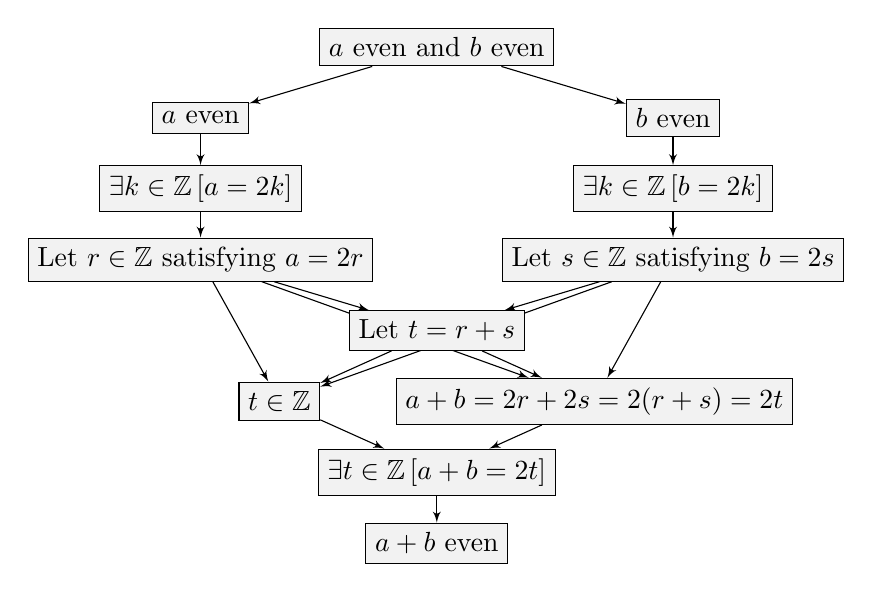
\begin{tikzpicture}
\node [block] (p1) at (0,0) {$a$ even and $b$ even};
\node [block] (p2) at (-3,-.9*1) {$a$ even};
\node [block] (p3) at (3,-.9*1) {$b$ even};
\path [line] (p1) -- (p2);
\path [line] (p1) -- (p3);
\node [block] (p4) at (-3,-.9*2) {$\exists k \in \mathbb{Z}\, [a=2k]$};
\node [block] (p5) at (3,-.9*2) {$\exists k \in \mathbb{Z}\, [b=2k]$};
\path [line] (p2) -- (p4);
\path [line] (p3) -- (p5);
\node [block] (p6) at (-3,-.9*3) {Let $r \in \mathbb{Z}$ satisfying $a=2r$};
\node [block] (p7) at (3,-.9*3) {Let $s \in \mathbb{Z}$ satisfying $b=2s$};
\path [line] (p4) -- (p6);
\path [line] (p5) -- (p7);


\node [block] (p9) at (-2,-.9*5) {$t \in \mathbb{Z}$};-
\node [block] (p10) at (2,-.9*5) {$a+b=2r+2s=2(r+s)=2t$};
\path [line] (p6) -- (p9);
\path [line] (p7) -- (p9);
\path [line] (p6) -- (p10);
\path [line] (p7) -- (p10);

\node [block] (p8) at (0,-.9*4) {Let $t=r+s$};
\path [line] (p6) -- (p8);
\path [line] (p7) -- (p8);

\path [line] (p8) -- (p9);
\path [line] (p8) -- (p10);

\node [block] (p11) at (0,-.9*6) {$\exists t \in \mathbb{Z}\,[a+b=2t]$};
\path [line] (p9) -- (p11);
\path [line] (p10) -- (p11);

\node [block] (p12) at (0,-.9*7) {$a+b$ even};
\path [line] (p11) -- (p12);
\end{tikzpicture}
\end{center}
The corresponding proof follows.
\begin{proof}
Let $a$ be even and $b$ be even. We want to prove $a+b$ is even. Since $a$ is even, there exists an integer $k$ such that $a=2k$. So, let $r$ be an integer satisfying $a=2r$. Since $b$ is even, there exists an integer $k$ such that $b=2k$. So let $s$ be an integer satisfying $b=2s$.

Let $t=r+s$. Since $r$ and $s$ are integers, $t$ is an integer. By substitution, $a+b=2r+2s=2(r+s)=2t$. So there exists an integer $t$ such that $a+b=2t$. Therefore, $a+b$ is even.
\end{proof}
Recall from Section~\ref{section:predicates-quantifiers} that the quantified variable is a placeholder variable, so writing $\exists k \in \mathbb{Z} [c=2k]$ is the same as writing $\exists u \in \mathbb{Z} [c=2u]$. Let's insist on using a new variable every time we have a quantifier. Then the flowchart is:
\begin{center} 
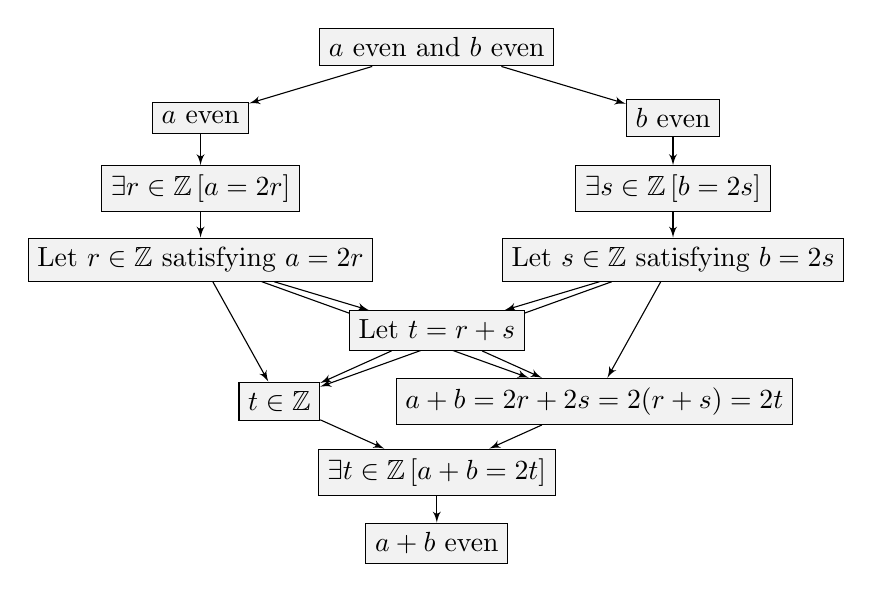
\begin{tikzpicture}
\node [block] (p1) at (0,0) {$a$ even and $b$ even};
\node [block] (p2) at (-3,-.9*1) {$a$ even};
\node [block] (p3) at (3,-.9*1) {$b$ even};
\path [line] (p1) -- (p2);
\path [line] (p1) -- (p3);
\node [block] (p4) at (-3,-.9*2) {$\exists r \in \mathbb{Z}\, [a=2r]$};
\node [block] (p5) at (3,-.9*2) {$\exists s \in \mathbb{Z}\, [b=2s]$};
\path [line] (p2) -- (p4);
\path [line] (p3) -- (p5);
\node [block] (p6) at (-3,-.9*3) {Let $r \in \mathbb{Z}$ satisfying $a=2r$};
\node [block] (p7) at (3,-.9*3) {Let $s \in \mathbb{Z}$ satisfying $b=2s$};
\path [line] (p4) -- (p6);
\path [line] (p5) -- (p7);


\node [block] (p9) at (-2,-.9*5) {$t \in \mathbb{Z}$};-
\node [block] (p10) at (2,-.9*5) {$a+b=2r+2s=2(r+s)=2t$};
\path [line] (p6) -- (p9);
\path [line] (p7) -- (p9);
\path [line] (p6) -- (p10);
\path [line] (p7) -- (p10);

\node [block] (p8) at (0,-.9*4) {Let $t=r+s$};
\path [line] (p6) -- (p8);
\path [line] (p7) -- (p8);

\path [line] (p8) -- (p9);
\path [line] (p8) -- (p10);

\node [block] (p11) at (0,-.9*6) {$\exists t \in \mathbb{Z}\,[a+b=2t]$};
\path [line] (p9) -- (p11);
\path [line] (p10) -- (p11);

\node [block] (p12) at (0,-.9*7) {$a+b$ even};
\path [line] (p11) -- (p12);
\end{tikzpicture}
\end{center}
The corresponding proof follows:
\begin{proof}
Let $a$ be even and $b$ be even. We want to prove $a+b$ is even. Since $a$ is even, there exists an integer $r$ such that $a=2r$. So, let $r$ be an integer satisfying $a=2r$. Since $b$ is even, there exists an integer $s$ such that $b=2s$. So let $s$ be an integer satisfying $b=2s$.

Let $t=r+s$. Since $r$ and $s$ are integers, $t$ is an integer. By substitution, $a+b=2r+2s=2(r+s)=2t$. So there exists an integer $t$ such that $a+b=2t$. Therefore, $a+b$ is even.
\end{proof}

Then, it seems a bit redundant to have ``there exists...'' as well as the  
``let ... satisfying ...'' ... so let's just keep one, but not the other. 
(We'll keep the ``there exists'' sentence. Must use new var each time.)

\begin{center}
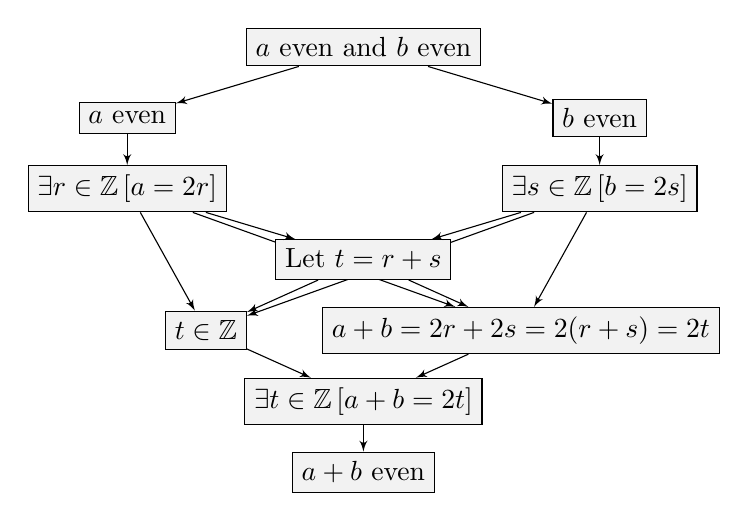
\begin{tikzpicture}
\node [block] (p1) at (0,0) {$a$ even and $b$ even};
\node [block] (p2) at (-3,-.9*1) {$a$ even};
\node [block] (p3) at (3,-.9*1) {$b$ even};
\path [line] (p1) -- (p2);
\path [line] (p1) -- (p3);
\node [block] (p4) at (-3,-.9*2) {$\exists r \in \mathbb{Z}\, [a=2r]$};
\node [block] (p5) at (3,-.9*2) {$\exists s \in \mathbb{Z}\, [b=2s]$};
\path [line] (p2) -- (p4);
\path [line] (p3) -- (p5);

\node [block] (p9) at (-2,-.9*4) {$t \in \mathbb{Z}$};-
\node [block] (p10) at (2,-.9*4) {$a+b=2r+2s=2(r+s)=2t$};
\path [line] (p4) -- (p9);
\path [line] (p5) -- (p9);
\path [line] (p4) -- (p10);
\path [line] (p5) -- (p10);

\node [block] (p8) at (0,-.9*3) {Let $t=r+s$};
\path [line] (p4) -- (p8);
\path [line] (p5) -- (p8);

\path [line] (p8) -- (p9);
\path [line] (p8) -- (p10);

\node [block] (p11) at (0,-.9*5) {$\exists t \in \mathbb{Z}\,[a+b=2t]$};
\path [line] (p9) -- (p11);
\path [line] (p10) -- (p11);

\node [block] (p12) at (0,-.9*6) {$a+b$ even};
\path [line] (p11) -- (p12);
\end{tikzpicture}
\end{center}

\begin{proof}
Let $a$ be even and $b$ be even. We want to prove $a+b$ is even. Since $a$ is even, there exists an integer $r$ such that $a=2r$. Since $b$ is even, there exists an integer $s$ such that $b=2s$.

Let $t=r+s$. Since $r$ and $s$ are integers, $t$ is an integer. By substitution, $a+b=2r+2s=2(r+s)=2t$. Because there exists an integer $t$ such that $a+b=2t$, we conclude $a+b$ is even.
\end{proof}

For additional practice, prove these two theorems:
\begin{theorem}
If $m$ is even and $n$ is odd, then $m+n$ is odd.
\end{theorem}
\begin{theorem}
If $j$ is even and $k$ is even, then $j-k$ is even.
\end{theorem}

The following definition is a generalization of even:
\begin{bdefinition}{Divides}{divides}
We say the integer $a$ \defn{divides}\index{divides} the integer $b$ if there exists an integer $k$ such that $b=ak$. We write $a \mid b$ to denote $a$ divides $b$.
\end{bdefinition}
This notion generalizes evenness since $b$ is even if and only if $2$ divides $b$.
\begin{blanguage}{}{}
This is a good time to remind all readers to follow the main habits for a definition. Following Habit~\ref{habit:part-of-speech}, is ``divides'' a noun, verb, or adjective? The word ``divides'' is a verb. Moreover, it is a transitive verb (meaning this is a verb which performs an ``action'' onto an object).
\end{blanguage}
\begin{bwarning}{Divides versus divided by}{divides-divided-by}
We have defined the transitive verb ``divides'' above, but do not confuse this with the phrase ``divided by.'' While there is a strong similarity in spelling, treat these as \emph{completely} different. The statement \fbox{$3$ divides $12$} is a proposition, and a true one at that. In contrast, the phrase \fbox{$3$ divided by $12$} is not a proposition because this is neither true nor false. In fact, $3$ divided by $12$ is just the number $\frac14$, once reduced.
\end{bwarning}

\begin{exercise}
In Exercise~\ref{exercise:disjunction-checklist}, you were asked to consider what are things that must be addressed in writing a definition of disjunction. Similarly, what are things that you must address when writing a definition for divides?
\end{exercise}

\begin{theorem}\label{theorem:divides-difference}
If $m$ divides $c$ and $m$ divides $d$, then $m$ divides $c-d$.
\end{theorem}
\begin{proof}
Suppose $m$ divides $c$ and $m$ divides $d$. We want to prove $m$ divides $c-d$. Since $m$ divides both $c$ and $d$, there exist integers $a$ and $b$ such that $c=ma$ and $d=mb$. Let $u=a-b$. Then $u \in \mathbb{Z}$ and $c-d=ma-mb=m(a-b)=mu$, so $m$ divides $c-d$.
\end{proof}

\begin{bwarning}{Do not divide when working just with integers}{}
It is tempting to want to write things like $r = \frac{t}{u}$ in the course of a proof involving only integers (as is the case when dealing with the definitions of even, odd, and divides). By applying division, however, you end up making it less clear which quantities are integers. If you are tempted to write $r =\frac{t}{u}$, then write $ru=t$ instead: every equation involving division/fractions can always be rewritten in terms of multiplication instead.
\end{bwarning}

\begin{bremark}{Existence does not always use the set of integers}{}
Because our first full examples of proof deal with the existence of quantified variable in $\mathbb{Z}$, it sometimes becomes a habit to always assume that existence deals with integers. However, if $S$ is a set (even if $S$ is not a set of integers, and even if $S$ is not even a set of a numbers), it is possible to prove statements that begin ``there exists $m \in S$ such that ...'' and it would be incorrect (in general) to say ``there exists an integer $m$ such that ...''. This kind of language could be used if $S$ was known to be a set of integers (or the set of all integers).
\end{bremark}

\begin{exercise}
Prove: If $x$ is even and $y$ is even, then $xy$ is even.\quad\quad\href{https://www.sharelatex.com/project/59ceb69336e6671a14199af2}{{\color{red}[key]}}
\end{exercise}

\begin{exercise}
Prove: If $k$ is even and $n$ is odd, then $kn$ is even.\quad\quad\href{https://www.sharelatex.com/project/59ceb6b336e6671a14199b04}{{\color{red}[key]}}
\end{exercise}

\begin{exercise}
Prove: If $k$ is odd and $p$ is odd, then $kp$ is odd.\quad\quad\href{https://www.sharelatex.com/project/59ceb6f236e6671a14199b0e}{{\color{red}[key]}}
\end{exercise}

\begin{exercise}
Prove: if $a$ divides $b$ and $b$ divides $c$, then $a$ divides $c$.
\end{exercise}

\subsection{Proving/using universally-quantified statements}\label{section:proving-using-forall}
%Save proving/using ``for all'' statements until after integer-related proofs are done
%Proving for all $x \in S$ (with mention of the $S$). This was a reminder to discuss the situation when there is \emph{now} a universe of discourse mentioned. In this text, we *always* have that situation.

Let $P(x)$ be the predicate ``$x$ breathes.'' Recall that we use $\mathbb{H}$ denote the set of all [living] humans. Let us assume that $\forall x \in \mathbb{H}\,[P(x)]$ is true. (Actually, it probably doesn't need to be \emph{assumed}: it probably is true that every human has picked their boogers.) Let $y$ denote your math instructor. Then $y \in \mathbb{H}$. Given the fact $\forall x \in \mathbb{H}\,[P(x)]$ and given the fact $y \in \mathbb{H}$, what can we conclude? We can conclude that your math instructor breathes. In other words, we conclude $P(y)$.

Every time you have a universally-quantified statement which is true, as soon as you know you have an element $y$ in the universe of discourse which was mentioned, then you get a fact about the individual $y$. In a flowchart:
\begin{bmethod}{Using a universally-quantified statement}{using-forall}
To use $\forall x \in U\,[P(x)]$, follow:
\begin{center}
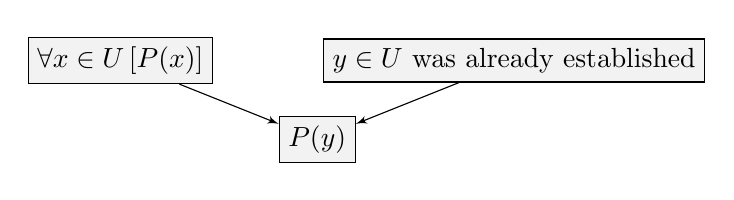
\begin{tikzpicture}
\node at (0,.3) {};
\node [block] (forall) at (-2.5,0) {$\forall x \in U\,[P(x)]$};
\node [block] (yinU) at (2.5,0) {$y \in U$ was already established};
\node [block] (Pofy) at (0,-1) {$P(y)$};
\path [line] (forall) -- (Pofy);
\path [line] (yinU) -- (Pofy);
\node at (0,-1.3) {};
\end{tikzpicture}
\end{center}
\end{bmethod}

\begin{bwarning}{}{}
To use a universally-quantified statement, we emphasize that you must already have an element $y$ which was already known to be in $U$. This is why we stated the phrase ``was already established'' in the flowchart above. You cannot just say ``Let $y \in U$.''
\end{bwarning}
The flowchart presented in Method~\ref{method:using-forall} allows us to start with a general fact (``$P(x)$ holds for all $x \in U$'') and combined with knowing of an object $y$ in the universe of discourse (example: $y$ is known to belong to $U$) allows us to conclude that $P(y)$ holds. This takes us from a general fact to a specific fact about a specific individual named $y$. It is general to say, ``Everyone breathes'' and it is specific to say, ``Your math teacher breathes.'' There will be times in our proof we will need to be that specific, and this flow chart helps us do this.

\begin{example}
Suppose we know \fbox{$\forall v \in D [P(v)]$} is true. Suppose we also know \fbox{$s \in D$} is true. Then we can conclude \fbox{$P(s)$} is true. Notice that our conclusion does not have the ``for all'' symbol.
\end{example}
\begin{example}
Suppose we know \fbox{$\forall h \in L [P(h)]$} is true. Suppose we also know \fbox{$z \in E$} is true. Then we cannot conclude anything based on these two facts, because we need something in $L$ to use $\forall h \in L [P(h)]$.
\end{example}

\begin{example}
Suppose we know \fbox{for all $b \in C$, the manager gives $b$ a raise} is true. Suppose we also know \fbox{$m \in C$} is true. Then we can conclude \fbox{the manager gives $m$ a raise} is true. Notice that the words ``for all'' are not in the conclusion.
\end{example}
\begin{example}
Suppose we know \fbox{for all $b \in C$, the manager gives $b$ a raise} is true. Suppose we also know \fbox{$b \in S$} is true. Then we cannot conclude anything based on these two facts, because we need something in $C$.
\end{example}
\begin{example}
Suppose we know \fbox{for all $x \in S$, a delivery for $x$ is available} is true. Suppose we also know \fbox{$y \in S$} is true. Then we can conclude \fbox{a delivery for $y$ is available} is true. Notice that the words ``for all'' are not in the conclusion.
\end{example}
\begin{example}
Suppose we know \fbox{for all $j \in J$, if $\pi > 2$, then Alex buys a bike from $j$}. Even though we know $\pi > 2$ is true, we can't really use \fbox{for all $j \in J$, if $\pi > 2$, then Alex buys a bike from $j$} yet, because it's stuck ``behind'' a `for all' statement. Say that we also knew $c \in J$. Then we could first conclude the implication \fbox{if $\pi > 2$, then Alex buys a bike from $c$} and by applying modus ponens, we further conclude \fbox{Alex buys a bike from $c$} is true.
\end{example}
\begin{example}
Suppose we know \fbox{for all $m \in A$, there exists $r \in B$ such that $m$ gives $r$ money} is true. Suppose we also know \fbox{$z \in A$} is true. Then we can conclude \fbox{there exists $r \in B$ such that $z$ gives $r$ money} is true. From this conclusion, Method~\ref{method:using-exists} applies and further conclusions can be made.
\end{example}

\begin{example}
If we know $\forall x \in G, xy=yx$ and we also know $z \in G$, then we can conclude $zy=yz$. In more detail, the predicate $P(x)$ is $xy=yx$. Since $z$ is already known to be in $G$, we can conclude $P(z)$, which is $zy=yz$.
\end{example}
\begin{example}
If we know $\forall x \in G, xy=yx$ and we know $y \in G$, we can conclude $yy=yy$. Note we replaced all the $x$'s with $y$'s.
\end{example}
\begin{example}
What can we conclude if we know $\forall x \in G, xy=yx$ when we also have $x \in G$? Here, the $x$'s are different in meaning. Since the $x$'s in $\forall x \in G, xy=yx$ are placeholder variables, it may help to replace the $x$'s with $u$'s, so that we can say we know $\forall u \in G, uy=yu$. Then with $\forall u \in G, uy=yu$, combined with the fact $x \in G$, we can conclude $xy=yx$.
\end{example}
\begin{example}
What can we conclude if we know $\forall x \in G, xy=yx$ and we know $x \in K$? Nothing. The universally-quantified statement says that something is true for each member of the set $G$. However, the $x$ we know about is in $K$. Do not let the fact that both of these statements use $x$ cause confusion. In fact, the first statement can be restated as $\forall u \in G, uy=yu$ by replacing all the placeholder variables.
\end{example}
\begin{example}
For a more stark example, if we know $\forall a \in B, a^{4}=1$ and we know that $c \in D$, then we can conclude nothing. Note that $\forall a \in B, a^{4}=1$ is the same statement as $\forall c \in B, c^{4}=1$. For the same reason that the $a$'s in $\forall a \in B, a^{4}=1$ are unrelated to the $c \in D$, the $c$'s in $\forall c \in B, c^{4}=1$ are unrelated to $c \in D$.
\end{example}

In writing proofs, some people like to use the phrase ``in particular\index{in particular}'' when using a universally-quantified statement.
\begin{example}
To use the statement $\forall r \in \mathbb{R}\,\exists s \in \mathbb{Z}\,s>r$ we will need to have a real number. For example, let's have in mind the real number $\pi$. In the form of a flowchart, here's what we can conclude:
\begin{center}
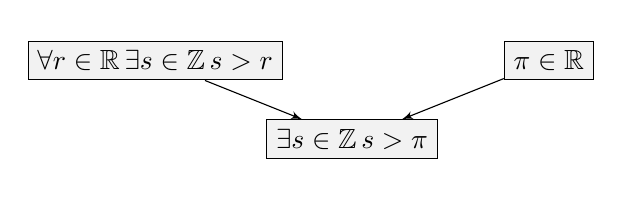
\begin{tikzpicture}
\node at (0,.3) {};
\node [block] (forall) at (-2.5,0) {$\forall r \in \mathbb{R}\,\exists s \in \mathbb{Z}\,s>r$};
\node [block] (yinU) at (2.5,0) {$\pi \in \mathbb{R}$};
\node [block] (Pofy) at (0,-1) {$\exists s \in \mathbb{Z}\,s> \pi$};
\path [line] (forall) -- (Pofy);
\path [line] (yinU) -- (Pofy);
\node at (0,-1.3) {};
\end{tikzpicture}
\end{center}
So note that $\forall r \in \mathbb{R}\,\exists s \in \mathbb{Z}\,s>r$ is a general statement. No matter what real number $r$ is, the statement $\exists s \in \mathbb{Z}\,s>r$ is true. But that statement is so general. For a specific statement, we should think of a particular real number, and we get the statement $\exists s \in \mathbb{Z}\,s> \pi$. We have already used the word particular (which has practically synonymous with ``specific'' as used here.)

How would the wording in a proof look? Suppose we had the sentence ``For all reals $r$, there exists an integer $s$ such that $s>r$.'' Then, the next sentence of our proof might be written, ``In particular, there exists an integer $s$ such that $s > \pi$.''
\end{example}

We have discussed how to use a universally-quantified statement. How would we prove a universally-quantified statement? 

Let $V$ be the set of all mountains in the United States with an elevation above $15000$ feet. Let $Q(x)$ be the predicate ``$x$ has a tree on it.''  How would we prove $\forall x \in V\,[Q(x)]$? In other words, how would we convince someone that every mountain with an elevation above $15000$ feet in the United States has a tree on it? Fortunately, there are not so many mountains with an elevation above $15000$ feet, so we could start with the Denali (the tallest) and keep going through each possible choice for $x$ one by one until we have seen all seven possible values for $x$. Each time, we can name the mountain and verify for the reader of our proof that $x$ has a tree on it.

Let $U$ be the set of all squirrels in Russia. Let $P(x)$ the predicate ``$x$ has brown eyes.'' How would we prove a statement like $\forall x \in U\,[P(x)]$? Maybe ``prove'' is too strong of a word to use here, but how would we convince someone that $\forall x \in U\,[P(x)]$ is true? Could we approach this in the same way as the tall mountains in the United States? Probably not. There are probably too many squirrels in Russia. Instead, imagine that we ask the reader to select any Russian squirrel they like. (In order for us to refer to the squirrel they picked, we'll call that squirrel $r$, and we'll state this in words by writing, ``Let $r \in U$ be arbitrary.'') Note that $r$ is a single squirrel. Then, suppose we write a proof which convinced the reader that $P(r)$ is true, in other words, that $r$ has brown eyes.

If we succeed in doing this, the reader should be convinced that $\forall x \in U\,[P(x)]$ is true. Now either the reader of our proof or an independent observer might say, ``But wait! The reader only picked one squirrel!'' The point is that the reader can go back and ``rewind the tape'' in the sense of Remark~\ref{remark:rewind-the-tape} and select a new squirrel: the reader goes back to the point in the proof which said ``Let $r \in U$ be arbitrary'' and selects a different squirrel to be $r$. Then, if the argument still applies and the reader sees that $P(r)$ is true, the reader can rewind again and select a new $r$. But if the reader does the thought experiment to see that no matter which $r \in U$ is selected, $P(r)$ is true, then the reader is now convinced that for \emph{all} $x$ in $U$, we have $P(x)$. This discussion leads to the following general method for proving a universally-quantified statement:
\begin{bmethod}{Proving a universally-quantified statement}{proving-forall}
To prove $\forall x \in U\,[P(x)]$, follow:
\begin{center}
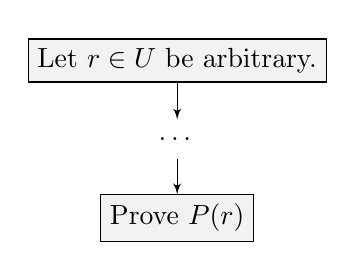
\begin{tikzpicture}
\node at (0,.3) {};
\node [block] (assume-p) at (0,0) {Let $r \in U$ be arbitrary.};
\path [line] (assume-p) -- (0,-.75);
\node at (0,-1) {$\dots$};
\node [block] (q) at (0,-2) {Prove $P(r)$};
\path [line] (0,-1.25) -- (q);
\node at (0,-1.3) {};
\end{tikzpicture}
\end{center}
\end{bmethod}

\begin{bmethod}{Proving a universally-quantified statement: a summary}{proving-forall-summary}
Method~\ref{method:direct-proof-method} said to prove the implication $p \rightarrow q$, you first assume $p$ is true, then use rules of inference to prove $q$ is true. Something is assumed (namely $p$).
\vskip6pt
In the same way, when proving $\forall x \in U\,[P(x)]$ we start by assuming we have a ``random'' element from the set $U$. This is accomplished by writing ``Let $r \in U$ be arbitrary'' as long as $r$ is a variable that has not yet been used in our proof. Then, using rules of inference, we must prove $P(r)$.
\end{bmethod}

\begin{blanguage}{What does the word ``arbitrary mean?}{arbitrary-meaning}
The purpose of the word ``arbitrary'' is really meant to be a reminder that the person \emph{reading} the proof (not the person writing the proof) may really choose whichever element from $U$ they like to be $r$. Instead of writing ``Let $r \in U$ be arbitrary,'' this may be shortened to just writing ``Let $r \in U$.'' There is no change in meaning. The point is that the sentence ``Let $r \in U$'' -- should it end there with a period -- already allows the reader to pick whichever element from $U$ that they want to be called $r$, even without the subsequent words ``be arbitrary.'' However, the word ``arbitrary'' is meant to serve as \emph{emphasis} that the reader may pick.
\vskip6pt
Because the reader gets to pick \emph{whichever} element they want from $U$, and for the practical reason that a proof will need to be written, the reader's choice is called $r$, and then the proof writer then proves that $P(r)$ holds, this ends up proving $\forall x \in U\,[P(x)]$. The idea that the reader may make \emph{any} choice of $r \in U$ is why the for \emph{all} statement is true.
\end{blanguage}

\begin{bwarning}{Proving versus using a universally-quantified statement}{}
To prove $\forall x \in U\,[P(x)]$, the first sentence to write would be ``Let $r \in U$ be arbitrary'' as long as $r$ is so far unused in the present proof. Instead the first sentence could be ``Let $s \in U$ be arbitrary'' but then the proof is done once $P(s)$ is proved.
\vskip6pt
This is unlike \emph{using} the proposition $\forall x \in U\,[P(x)]$. To \emph{use} this proposition, you must already have an element in $U$ that you know of (which we have called $y$ in our earlier flowchart and discussion). Using $\forall x \in U\,[P(x)]$ should \emph{never} have a sentence of the form ``Let $y \in U$ be arbitrary.''
\end{bwarning}

\begin{example}
Say you need to prove $\forall v \in D [P(v)]$. As long as $s$ has not been used, write \fbox{Let $s \in D$}. Then work to prove \fbox{$P(s)$}.
\end{example}
\begin{example}
Say you need to prove $\forall v \in D [P(v)]$. As long as $v$ has not been used, write \fbox{Let $v \in D$}. Then work to prove \fbox{$P(v)$}.
\end{example}
\begin{example}
Say you need to prove \fbox{for all $b \in C$, the manager gives $b$ a raise} is true. As long as $b$ has not been used in your proof, write \fbox{Let $b \in C$}. Then work to prove \fbox{the manager gives $b$ a raise}.
\end{example}
\begin{example}
Say you need to prove \fbox{for all $b \in C$, the manager gives $b$ a raise} is true. Suppose that the letter $b$ is already used up. As long as $m$ has not been used in your proof, write \fbox{Let $m \in C$}. Then work to prove \fbox{the manager gives $m$ a raise}.
\end{example}
\begin{example}
Let's say the task is that you need to prove \fbox{for all $x \in S$, a delivery for $x$ is available} is true. Let's say that the letter $r$ has not been used yet in your proof. Then write \fbox{Let $r \in S$ be arbitrary} which allows the reader to pick any element from the set $S$ that they want, and you will refer to their choice by the variable $r$. Then you need to prove \fbox{a delivery for $r$ is available} is true.
\end{example}

\begin{example} % forall implication
Say we need to prove \fbox{for all $a \in A$, if $a$ likes to sew, then $a$ rides motorcycles}. As long as $b$ hasn't been used in the proof yet, we would write \fbox{Let $b \in A$ be arbitrary.} then we would need to prove \fbox{if $b$ likes to sew, then $b$ rides motorcycles}, so we would assume \fbox{$b$ likes to sew} and work to prove \fbox{$b$ rides motorcycles}.
\end{example}
\begin{example} % forall exists
Say we need to prove \fbox{$\forall x \in U \exists y \in V [ Q(x,y) ]$}. It may help to write extra brackets for this, for now, taking it one step at a time. To prove \fbox{$\forall x \in U [\exists y \in V [ Q(x,y) ]]$} we should first write \fbox{Let $r \in U$ be arbitrary} as long as $r$ hasn't been used in our proof. Then we would need to prove \fbox{$\exists y \in V [ Q(r,y) ]$}. Connecting this back to Method~\ref{method:proving-forall}, the $P(x)$ that appears there is \fbox{$\exists y \in V [ Q(r,y) ]$} here.
\end{example}
\begin{example} % forall exists
Say we need to prove \fbox{for all $m \in A$, there exists $r \in B$ such that $m$ gives $r$ money}. This is really in the same general structure/shape as the previous example, but in words. Then we would start by writing \fbox{Let $m \in A$ be arbitrary} as long as $m$ hasn't been used. (Otherwise, pick a variable that hasn't been mentioned in the proof yet.) Then we would work to prove \fbox{there exists $r \in B$ such that $m$ gives $r$ money}.
\end{example}

\begin{example}
Say we need to prove \fbox{for all $h \in S$, if $h$ has a cat, then $h$ is photographer}. As long as $h$ is unused so far in our proof, then our proof of this statement would start \fbox{Let $h \in S$ be arbitrary.}. This allows the reader of our proof to pick their favorite element of $S$ and call it $h$. Then we would need to prove \fbox{if $h$ has a cat, then $h$ is photographer} which we could signal in the text of our proof by writing \fbox{We will prove if $h$ has a cat, then $h$ is photographer.} with emphasis here on the words ``we will prove'' because we haven't proven this implication at this point yet. Then to prove this implication, following Method~\ref{method:proving-implication-direct}, we would write \fbox{Suppose $h$ has a cat.} and then we would work to prove \fbox{$h$ is a photographer}.
\end{example}






\begin{example}
Suppose that we were given the task to prove ``For all $m \in U$, there exists an $n \in L$ such that $n \geq m$.'' This task will be a bit impossible here only because we were not told what set $U$ was nor what set $L$ was. Nevertheless, the format of proving this statement would be as follows. We would start by writing ``Let $m \in U$ be arbitrary'' or can just write ``Let $m \in U$'' for short. Then, one can include the optional sentence ``We will show that there exists an $n \in L$ such that $n \geq m$.''

At the end of the proof, there will probably a sentence like ``Therefore, there exists an $n \in L$ such that $n \geq m$,'' but this very likely not be the sentence immediately after the ``We will show...'' sentence.
\end{example}

The examples above show that in a proof, it is necessary to address the quantifiers in the order in which they appear. From Section~\ref{section:nested-quantifiers} it is generally incorrect to swap quantifiers.


For a complete example, let us examine the following theorem:
\begin{theorem}\label{theorem:forall-a-if-b-div-c}
For all $a \in \mathbb{Z}$, if $b$ divides $c$, then $b$ divides $ac$.
\end{theorem}
\begin{proof}
Let $a \in \mathbb{Z}$ be arbitrary. We will prove that if $b$ divides $c$, then $b$ divides $ac$.

To prove that $b$ divides $c$ implies that $b$ divides $ac$, let us suppose that $b$ divides $c$. We will prove that $b$ divides $ac$. Since $b$ divides $c$, both $b$ and $c$ are integers and there exists an integer $d$ such that $bd=c$. Let $z=ad$. Then $z$ is an integer, and $bz=b(ad)=bad=abd=a(bd)=ac$. Since $z$ is an integer and $bz=ac$, we have proved that $b$ divides $ac$.

The previous paragraph proved that if $b$ divides $c$, then $b$ divides $ac$. Since the selection of $a \in \mathbb{Z}$ was arbitrary, we have proved that for all $a \in \mathbb{Z}$, if $b$ divides $c$, then $b$ divides $ac$.
\end{proof}

\begin{theorem}\label{theorem:universal-first-decontextualized-training}
If
\begin{itemize}
\item For all $a \in B$, if $a$ does not play chess, then $a$ does not bike to school.
\item For all $j \in T$, if $j$ likes ketchup, then $j$ bikes to school.
\item If $c \in S$, then $c \in T$.
\item If $m \in T$, then $m \in B$.
\end{itemize}
then: For all $r \in S$, if $r$ likes ketchup, then $r$ plays chess.
\end{theorem}
\begin{proof}
Let $r \in S$ be arbitrary. We want to prove if $r$ likes ketchup, then $r$ plays chess. So suppose $r$ likes ketchup. We will prove $r$ plays chess. Recall $r \in S$, so by the third hypothesis, we can say $r \in T$ by modus ponens. Since $r \in T$, by the second hypothesis, if $r$ likes ketchup, then $r$ bikes to school. Since $r$ likes ketchup, we conclude $r$ bikes to school. Recall $r \in T$, so by the fourth hypothesis, $r \in B$. Since $r \in B$, and the first hypothesis is a ``for all'' statement we now get to use, we know if $r$ does not play chess, then $r$ does not bike to school. But we saw $r$ bikes to school, so by modus tollens, $r$ plays chess.
\end{proof}

\begin{theorem}
Assuming the hypotheses
\begin{itemize}
\item H1: For all $r \in M$, if $r$ is vegetarian, then $r$ makes ceramic vases.
\item H2: If $w$ makes ceramic vases, then there exists an $f \in Q$ such that $w$ mails a gift to $f$.
\item H3: If $z \in X$, then $z$ is vegetarian.
\item H4: If $g \in Q$, then $g \in Y$.
\item H5: Every element of $X$ is an element of $M$.
\end{itemize}
then, for all $b \in X$, there exists $c \in Y$ such that $b$ mails a gift to $c$.
\end{theorem}
\begin{proof}
Let $b \in X$ be arbitrary. We want to prove there exists $c \in Y$ such that $b$ mails a gift to $c$, for then we would be done. Since $b \in X$, by H3 and modus ponens, $b$ is vegetarian. Since $b \in X$, by H5 we have $b \in M$. Since $b \in M$, applying H1, we learn that $b$ is vegetarian implies $b$ makes ceramic vases. Since we already saw $b$ is vegetarian, by modus ponens, $b$ makes ceramic  vases. Using this with modus ponens on H2, we conclude there exists an $f \in Q$ such that $b$ mails a gift to $f$. Let $c = f$. Since $c \in Q$, we conclude $c \in Y$ by H4. Since $c \in Y$ and since $b$ mails a gift to $c$, we have shown that there exists a $c \in Y$ such that $b$ mails a gift to $c$.
\end{proof}

\begin{exercise}
Prove: For all integers $a$ and $b$, if there is an integer $c$ such that $10c=a-b$, then there is an integer $d$ such that $5d=b-a$.\quad\quad\href{https://www.sharelatex.com/project/59ceb71936e6671a14199b1e}{{\color{red}[key]}}
\end{exercise}

\begin{exercise}
Use the following hypotheses:
\begin{itemize}
\item H1: If $r$ likes Disneyland, then $r$ is an element in the set $S$.
\item H2: For all $c \in P$, if $c$ walks to school, then $c$ is a rock climber.
\item H3: Every element in the set $M$ is an element in the set $P$. (So $x \in M$ implies $x \in P$. Similarly, $z \in M$ implies $z \in P$.)
\item H4: If $b$ does not like Disneyland, then $b$ is not an element in the set $P$.
\item H5: For all $s \in S$, the person $s$ walks to school.
\end{itemize}
to prove the proposition: For all $m \in M$, the person $m$ is a rock climber.
\end{exercise}

\begin{exercise}
Prove the following statement: If $x$ is even and $y$ is odd, then $x-y$ is odd.
\end{exercise}
\begin{exercise}
Prove: For all integers $s$, if $s$ is even, then $s^3$ is even.
\end{exercise}
\begin{exercise}
Prove: For all integers $s$, if $s$ is odd, then $s^2$ is odd.
\end{exercise}
\begin{exercise}\label{exercise:contrapositive-squared-warmup}
What is the contrapositive of \fbox{If $s$ is odd, then $s^2$ is odd}? You may assume the fact that an integer that is not odd is even.
\end{exercise}
\begin{exercise}
Prove: If $a$ and $b$ are integers satisfying $2b^2=a^2$, then $a$ is even and $b$ is even. Hint: use Exercise~\ref{exercise:contrapositive-squared-warmup}.
\end{exercise}

\begin{exercise} % surjective preview
Assume the two hypotheses
\begin{itemize}
\item $\forall y \in B,\, \exists x\in A$ such that $P(x,y)$
\item $\forall z \in C,\, \exists y \in B$ such that $Q(y,z)$
\end{itemize}
to prove: for all $c \in C$, there exists an $a \in A$ such that $\exists b \in B$ such that $P(a,b) \wedge Q(b,c)$.
\end{exercise}

\begin{exercise} % injective preview
Assume the two hypotheses
\begin{itemize}
\item $\forall y_1 \in B\, \forall y_2 \in B\, \forall x_1 \in A\, \forall x_2 \in A$, if $y_1=y_2$ and $P(x_1,y_1)$ and $P(x_2,y_2)$, then $x_1=x_2$.
\item $\forall z_1 \in C\, \forall z_2 \in C\, \forall y_1 \in B\, \forall y_2 \in B$, if $z_1=z_2$ and $Q(y_1,z_1)$ and $Q(y_2,z_2)$, then $y_1=y_2$.
\end{itemize}
to prove: for all $c_1 \in C$, for all $c_2 \in C$, for all $b_1 \in B$, for all $b_2 \in B$, for all $a_1 \in A$, for all $a_2 \in A$, if $c_1=c_2$ and $P(a_1,b_1)$ and $P(a_2,b_2)$ and $Q(b_1,c_1)$ and $Q(b_2,c_2)$, then $a_1=a_2$.
\end{exercise}



%\begin{example}
%Using $\forall a \in R$, ... when you have $b \in R$
%\end{example}

\section{Intermission: comments on proofs}

By rereading the three proofs of Theorem~\ref{theorem:sum-of-evens} and the proof of Theorem~\ref{theorem:divides-difference}, notice each proof is written in complete sentences. A proof is a water-tight argument that starts from propositions which are assumptions and, following the rules of inference, convinces a reader of new propositions, eventually leading to a final proposition.

In a previous math class such as algebra or calculus, you were probably not expected to write in complete sentences. However, this old style of writing mathematics, while it can convey all of the key logic involved in a computation, is too primitive as a method of writing to convince a reader of the type of facts (theorems) that are truly proved in upper-level mathematics. We need complete sentences.

This type of writing, because it is new, will be challenging at first. You are encouraged to revisit this section and the previous sections in this chapter often, so that everything becomes more familiar. Chapter~\ref{chapter:methods-of-proof} is the core material of this handbook, and is the prerequisite to further chapters.
This section states many pieces of advice, tips, and expectations:

\begin{bhabit}{}{}
Write your proofs in complete sentences. (Some of the things we mention later will help with this process.)
\end{bhabit}

\begin{bhabit}{}{}
Every sentence in a proof ends in a period.
\end{bhabit}
In fact, each sentence of your proof should end with a period, even if the last portion of the sentence is notation, and even if the last portion is center-lined as larger block of notation. So, instead of writing \fbox{Let $a = x+y$} as a sentence, write \fbox{Let $a = x+y$.} with the period at the end.

\begin{bhabit}{}{}
If you are concerned about writing in complete sentences, remember that there are only several types of sentences that you will write.
\end{bhabit}
For example, if $p$, $q$, $r$, and $s$ are all propositions, your sentences will likely be of one of the following formats:
\begin{itemize}
\item $p$.
\item Since $p$, we have $q$. % since before
\item $q$ since $p$. % since after
\item Therefore, $q$ because $p$.
\item Because $p$,\,\,$q$.
\item So, $q$.
\item Thus, $q$.
\item Because $r$ and $s$, we conclude $q$.
\end{itemize}
It is understandable that those who feel comfortable with mathematical calculations as done in calculus might be squeamish at first regrading writing proofs. You might want to say, ``but I'm not a sentences-making person!'' Take heart in knowing that the sentences written for a proof are little more than propositions surrounding a few connecting words such as thus, because, since, therefore, we see that, hence, etc. For example, the proof of Theorem~\ref{theorem:sum-of-evens} had the sentence ``Since $a$ is even, there exists an integer $k$ such that $a=2k$.'' which is in the grammatical format of ``Since $p$, we have $q$.'' from our list above.


\begin{bhabit}{}{}
Remember that most of the hard work of a proof is in building the flowchart which is \emph{very} much using the same type of thinking you did when doing computational mathematics.
\end{bhabit}
The consistency of thought you have trained yourself to do in deciding between the Chain Rule versus the Quotient Rule has made you ready to build flowcharts of proof. Just as you can take the distributive law $a(b+c)=ab+ac$ to turn $5(a+b)$ into $5a+5b$, you can take the flow chart for modus ponens and see that if you already have $q \rightarrow s$ is true and you already have $q$ is true, you can conclude $s$ is true. Think of the ``variables'' you see in the flowcharts as propositions to substitute in, just the same as you need to substitute to use $a(b+c)=ab+ac$.


\begin{bhabit}{}{}
The order of sentences matters.
\end{bhabit}
Though you may have built the flowchart for your proof by discovering things in a different order, when turning your flowchart into the sentences of a proof, think about what relies on what. Consider a box in the flowchart, and note that you can only convince the reader that the proposition in that box is true only after having introduced the contents of the boxes pointing into this box: the arrows of your diagram can be thought of like the prerequisites for various classes in a major.


\begin{bhabit}{}{}
Keep sentences short.
\end{bhabit}
You do not need to worry about overly flowery language. Try to communicate one idea (or maybe two ideas) in a sentence. Often, long sentences are trying to communicate too many things, and often, the things that are attempting to be discussed wouldn't even belong in consecutive sentences! Break up long sentences into smaller sentences. (Once you have it so that each sentence is communicating one idea, it is easier to also think about what order the sentences should appear.)


\begin{bhabit}{}{}
Don't be afraid of having lots of scratch work, though you'll probably never present your scratch work.
\end{bhabit}
Clarify your task, then build a flowchart organizing the argument of the proof. A flowchart of proof logic involves \emph{lots} of scratch work! Do not be shy about having scratch work! You may have become so accustomed to the calculations done in calculus that you forgot a time when you used a lot of scratch work. (Remember the first time you computed slopes of secant lines, there was a lot of work to write out!) A cleanly-written proof is nice, but often so nice that it hides the fact that there were probably a lot of dead ends, restarts, and so on.


\begin{bhabit}{}{}
Build the pieces of the flowchart which you can. Then work on connecting pieces.
\end{bhabit}
Identifying what you need to prove (and looking up its flowchart) and identifying what you have not yet used (and looking up its flowchart). In our first example of a proof, we started with the first box and the box. Then we worked inward by creating the second box and the second-to-last box. Getting the main skeleton of the proof is half the battle!


\begin{bhabit}{}{}
Always keep track of whether you need to use a proposition or need to prove a proposition.
\end{bhabit}
For each type of proposition (conjunction, implication, existentially-quantified statement, universally-quantified statement, and so on), the flowchart templates for proving and using are different. If you need to use a statement but are attempting to prove that statement, things will not work out. Similarly, if you need to prove a statement but are attempting to use that statement, things will not work out.


\begin{bhabit}{}{}
If you're stuck, build intuition from a concrete example.
\end{bhabit}
As an example, let's say we were stuck at proving that the product of perfect squares is a perfect square. (We will need one new definition: an integer $r$ is a \defn{perfect square} if there exists an integer $x$ such that $x^2=r$.) We are looking to prove for all $r,s \in \mathbb{Z}$, if $r$ is a perfect square and $s$ is a perfect square, then $rs$ is a perfect square.

Of course the proof of this universally-quantified statement is going to start with ``Let $r \in \mathbb{Z}$ be arbitrary and let $s \in \mathbb{Z}$ be arbitrary'' followed by a sentence such as ``Suppose $r$ and $s$ are perfect squares.'' Because $r$ is a perfect square, there exists an integer $x$ such that $r=x^2$. Similarly, there exists an integer $y$ such that $s=y^2$. If we feel stuck in proving that $rs$ is a perfect square, we should build intuition from an example.

As our example, suppose $r=9$ and $s=25$. Then, the reason $r$ is a perfect square is that there exists an integer (namely $3$) such that $r=3^2$. Similarly, $s=5^2$. Connecting our example to the notation already introduced in our proof, $x=3$ and $y=5$. We need to prove $rs$ is a perfect square, and in our current example, that is the number $225$. When trying to prove $rs$ is a perfect square, need to prove that there exists $z \in \mathbb{Z}$ such that $rs=z^2$. Connecting to our example, we need to find an integer $z$ such that $225=z^2$. While $z$ needs to be $15$ in our specific example, how does this provide a hint for how we should define $z$ in our specific proof, only having access to $r$, $s$, $x$, and $y$? Notice that $15 = 3 \cdot 5$, so this suggests we should define $z$ to be $xy$. After checking, it seems this will work, so here is a complete proof:

Let $r \in \mathbb{Z}$ be arbitrary and let $s \in \mathbb{Z}$ be arbitrary. Suppose $r$ and $s$ are perfect squares. Because $r$ is a perfect square, there exists an integer $x$ such that $r=x^2$. Similarly, there exists an integer $y$ such that $s=y^2$. Let $z=xy$. Since the product of integers is an integer, $z \in \mathbb{Z}$. Then $rs = x^2 \cdot y^2 = (xy)^2 = z^2$. Since $z \in \mathbb{Z}$ and $rs=z^2$, we have proved that $rs$ is a perfect square.

Note that the example is not a proof. (The proof was the eight sentences of the previous paragraph.) However, the example helped us in defining $z$ to be $xy$, the key place where one usually gets stuck. Think of what is going on as a conversation. As the reader reads \fbox{Let $r \in \mathbb{Z}$ be arbitrary}, they might pick $r=31$. They might similarly pick $s=16$. Then, when the next sentence says ``Suppose $r$ and $s$ are perfect squares'' they need to go back, and choose differently. They might choose $r=9$ and $s=16$. From their choice of $r=9$, they would determine that $x$ could either be $3$ or $-3$, and in this manner, they could use their own example to help guide their \emph{reading} of the proof. However, the proof stands apart from any example. In fact, from the fact that they can pick $r$ and $s$ to be arbitrary perfect squares, they might ``rewind'' and choose $r=100$ and $s=121$. And once they read through the proof using $r=100$ and $s=121$, if they are still are still unconvinced, they could choose $r=144$ and $s=49$ and read through the proof again.

\begin{bhabit}{}{}
The language used to state propositions differs from the language in proofs.
\end{bhabit}
For example, to \emph{prove} a ``for all'' statement, your proof is going to contain text similar to ``Let $x \in A$ be arbitrary.'' However, keep in mind that the phrase ``For all $x \in A$, \dots'' is language used in \emph{stating} a proposition that you will prove, while ``Let \dots be arbitrary'' is very different language, and is used in \emph{proving} that statement.

As another example, suppose the statement to prove is an implication. Then, you might be \emph{proving} the statement ``If $p$ then $q$'' but your proof of this will probably not focus on using the words ``if'' and ``then.'' Instead, your proof will say something like ``Suppose $p$ is true.'' The word ``suppose'' is \emph{not} going to appear when you state the proposition.


\begin{bhabit}{}{}
Remember that using a proposition and proving a proposition are very different. %make an everyday example?
\end{bhabit}
\begin{center}
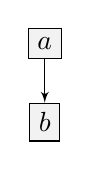
\begin{tikzpicture}
\node [block] (assume-p) at (0,0) {$a$};
\node [block] (q) at (0,-1) {$b$};
\path [line] (assume-p) -- (q);
\end{tikzpicture}
\end{center}
In the small flowchart above the proposition $a$ is being used, and the proposition $b$ is being proved. In fact, $a$ is used to prove $b$. On a very practical level, the methods used for proving and using an implication are very different, as seen from the very different looking flowcharts in Section~\ref{section:proving-using-implication}. Similarly, proving versus using a conjunction have very different flowcharts. Proving verses using an existentially-quantified statement have very different flowcharts. For each type of proposition, this occurs. You will waste time if you try to prove something that you should use. Similarly, you will waste time trying to use something that you should prove.

\begin{bhabit}{Do not use a characterization as a definition}{characterization-for-definition}
Do not use an ``alternate definition'' as a definition.
\end{bhabit}
Recall the definition of odd: an integer $m$ is odd if there exists an integer $s$ such that $m=2s+1$. While it turns out to be true that an integer $m$ is odd if and only if there exists an integer $k$ such that $m=2k-1$, do not use this as the definition. The fact that $m$ is odd if and only if there is an integer $k$ such that $m=2k-1$ is known as a \defn{characterization}\index{characterization} of being odd. A characterization should not replace the definition. (It is this characterization which we have called an ``alternate definition'' above.)

Think of each definition given as the \emph{original} source material. With each newly-introduced term, we have to start somewhere, and that is the definition. When you are asked to recite a definition, do not provide a characterization instead.

\begin{bhabit}{}{}
Do not bother writing ``by definition'' all the time.
\end{bhabit}

Perhaps this is a matter of taste, but if you were required to write ``by definition'' each time you needed a definition in your proofs, you would likely need to write ``by definition'' at least once (if not two or three times) per sentence. This would be too much clutter to include this all the time. There may be some key points of your proof where you would like to use this, but even in those cases, you might want to say something like ``by definition of $\varphi$'' or state ``by definition of the normal subgroup.''

Part of minimizing the expectation of writing ``by definition'' all the time points out a rather important aspect of proofs. You will need to reference definitions a lot! (This is why you hear your math instructor say ``Know your definitions'' so often: it is an essential part of proof.)

\begin{bhabit}{}{}
Be patient with yourself.
\end{bhabit}
The list above has many suggestions on things to work on, and it may take a while to master them all. Though the explanation of each point may be longer, the expectation or the advice consists of one or two short sentences. Connect the advice/expectations to the examples of proofs already given, and challenge yourself to work on one of these things at a time. You'll likely want to revisit this list and keep working on these things.

\subsection{The word ``let''}

We have used the word ``let'' in several different settings. We will discuss the various ways we have used the word ``let'' and provide a unified understanding of why the word is being used. There are three settings in our proofs where the word ``let'' has been used so far:
\begin{enumerate}
\item Using an existentially-quantified statement (Method~\ref{method:using-exists})

Initially, when using an existentially-quantified statement, the flowchart suggested writing a sentence like ``Let $b \in U$ satisfying $P(b)$.'' However, by the time we got to shorter proofs of Theorem~\ref{theorem:sum-of-evens}, we saw ways to avoid writing in such a lengthy manner. This was included for completeness, but it means that we are really only down to the next two uses of the word ``let.''

\item Proving an existentially-quantified statement (Method~\ref{method:proving-exists})

To prove that there exists an $x \in U$ such that $P(x)$, the flowchart says to define an object (which we called $c$). This is often done by writing something like ``Let $c=2r^3$'' or a similar statement. In the proof of Theorem~\ref{theorem:sum-of-evens}, we wrote ``Let $t=r+s$.'' At the time that we wrote this, note that $r$ and $s$ were already defined.

Later, once you are comfortable with proving existentially-quantified statements, you may get to a point where you define an object as needed, but without naming it using a variable such as $c$. In this sense, it would be possible to say that you can avoid writing things like ``Let $t =r+s$'' but for now, it would be good practice to write things like ``Let $t=r+s$.''

\item Proving a universally-quantified statement (Method~\ref{method:proving-forall})

To prove $\forall x \in U\, [P(x)]$, you must have a sentence such as ``Let $r \in U$ be arbitrary'' and then you would work towards proving $P(r)$. Writing ``Let $r \in U$ be arbitrary'' allows the reader to select any element of $U$ they want to, and their selection is referred to as $r$, so that you have a name by which to call the reader's selection from $U$.

Note that there is no use of the word ``let'' when \emph{using} a universally-quantified statement.
\end{enumerate}

These are the three situations in which you would use ``let'' in a proof, though you can avoid the first of these three. Thus, two situations remain. What does ``let'' mean? We use the word ``let'' in a proof to refer to some object later. When writing ``Let $t=r+s$'' there was already an $r$ and an $s$ which were introduced in the proof, and their sum was useful later on in the proof, so it helped to call $r+s$ something, and we chose to call it $t$. Instead of writing ``Let $t=r+s$'' we could have written ``We define $t$ to be $r+s$.'' Then, $t$ is mentioned later on in the proof. Finally, if you write the sentence ``Let $r \in U$ be arbitrary'' then the reader may fix $r$ to be any element from the set $U$. Just as in the previous example where $t$ would be mentioned later on in the proof, here, $r$ will be mentioned later in the proof.

In both of these situations, the word ``let'' allows the proof writer to define things which will be useful later. There was a time in the past when you used ``let'' although it might have been implicit. When evaluating
\[ \int (1-\sin^2 x)^3 \cos x\,dx\]
you had used substitution. While you may have just written \fbox{$u=\sin x$} in the past, this is really short for ``Let $u=\sin x$'' after which you ended up writing $u$ again when you wrote
\[ \int (1-u)^3\,du.\]
The word let should always be followed by variable that has not been used yet in your proof:
\begin{itemize}
\item Ensure that the variable you are defining appears \emph{immediately} after the word ``let.'' 

Write ``Let $t=r+s$'' instead of writing ``Let $r+s=t$.'' We are introducing $t$, and defining $t$ to be $r+s$.

\item Ensuring that the variable appears immediately after the word ``let'' also helps avoid a peculiar issue that might arise otherwise:

Suppose, we are in the middle of a proof, where $a$, $b$, $c$, and $d$ are all real numbers which have already been defined. Then if a proof has the sentence ``Let $3a + b^5 + \ln(3+c^2) - \sin(m) = m^5 + d$,'' the reader would (probably) interpret this to mean that the writing is trying to define $m$. However, it is not readily apparent that there even is \emph{any} possible choice for $m$ where $3a + b^5 + \ln(3+c^2) - \sin(m) = m^5 + d$ is true. In other words, what if the equation $3a + b^5 + \ln(3+c^2) - \sin(m) = m^5 + d$ has no solution for $m$? Writing like this becomes a difficult way to define the variable $m$, and insisting on the new variable appearing immediately after the word ``let'' will avoid this situation.

As a slightly different version of this, sometimes people will write ``Let $m$ be an integer such that $3a + b^5 + \ln(3+c^2) - \sin(m) = m^5 + d$.'' While this sentence follows the expectations written for the word ``let'' it has the same danger which was just mentioned. In fact, it is generally good to avoid writing a sentence in the form ``Let $m \in U$ be such that $P(m)$'' because this generally leads the reader to ask, ``Wait, is there even any $m \in U$ where $P(m)$ is true in the first place?'' The \emph{only} time to write this type of sentence is immediately after the reader has been convinced that $\exists z \in U\,[P(z)]$.

\item Be sure that ``let'' is followed by an \emph{unused} variable.

Otherwise, you would be redefining the variable. If your proof at some point said ``Let $m=3k+4$'' then the same proof should not later have the sentence ``Let $m=3k+5$.'' The reader would think, ``Wait! Earlier you told me that $m$ would be defined to be $3k+4$. Now you're saying that $m$ should be defined to be $3k+5$? Which is it?''

This would be redefining $m$. If you do need to define something to be $3k+5$, use a new variable.
\end{itemize}

\begin{bwarning}{}{}
While it is okay to write \fbox{Let $x = 7^2 + 3$} it is not okay to write \fbox{Let $x \in \mathbb{Z}$ such that $3x + 5 = 29-x^2$} (unless it comes immediately after an appropriate ``there exists'' statement) because there might not exist an integer $x$ which satisfies $3x + 5 = 29-x^2$.
\end{bwarning}
\begin{bwarning}{}{}
As another example of this, it is incorrect to write ``Let $x$ be a real such that $x^2+49 = 3-2x$.'' Note that even among real numbers $x$, there is no solution to the equation $x^2+49 = 3-2x$. Thus, writing a sentence in this format (Let $x$ ... such that ...) is dangerous because you as the writer may feel you have established something and want the reader to move on to the next thing, but nothing was established because there might not exist such an $x$. This is why the format of using `let' is to have `let' followed by a new variable (say $x$) followed by an equal sign, followed by an expression that is already defined (and therefore doesn't mention $x$). For example, writing ``Let $x=u^2+3$'' is okay, provided $u$ already is established.
\end{bwarning}

Contrast this with Method~\ref{method:using-exists}: if you already know $\exists x \in U$ such that $P(x)$, then it is okay to write \fbox{Let $x \in U$ such that $P(x)$}.

\subsection{Other concerns}

The higher-priority comments have been addressed earlier in this section, but there are other things to consider (some stylistic, some not) when writing mathematics.
\begin{itemize}
\item In formal mathematical writing, a sentence should not begin with notation.

Instead of writing \fbox{$f$ is continuous on the interval $[3,9]$.} in formal writing, one should write\\ \fbox{The function $f$ is continuous on the interval $[3,9]$.}\,. The additional words ``the function'' help to clarify what type of object we have.

There are situations when a less-than-formal style of writing is acceptable, but you will need to discuss this with your instructor. The typical situations for this are when time is of the essence (instructor's lecture, or students taking a quiz/test). In my own proof-based classes, writing\\ \fbox{$f$ is continuous on the interval $[3,9]$.} would be okay on a quiz but not in submitted homework.

\item Proofs will involve scratch work.

Be sure not to turn in scratch work as the proof. Your own process of discovering will involve writing propositions (in a flowchart) in a different order than you might present them in a proof. Your proof should demonstrate careful flow of logic. Related to this:

\item Each sentence should be readily apparent to the reader.

When proving the implication following Method~\ref{method:proving-implication-direct}, we would first suppose that $p$ is true. Then we eventually need to convince the reader that $q$ is true, but this might not occur right away. To indicate that this is where we are headed, we might include ``We will show that $q$ is true.'' A sentence of this kind is not strictly \emph{required}, but it helps the reader see where you are going in writing your proof. (In addition, while you are early in your proof-writing career, sentences like this help you on track of what you need to prove.)

As an example, see the proof of Theorem~\ref{theorem:odd-plus-odd-is-even}. After starting by supposing that $a$ is odd and that $b$ is odd, the next sentence cannot be ``The integer $a+b$ is even'' because the reader would not be convinced at this point that $a+b$ is even. We wrote ``We want to prove $a+b$ is even'' which is another way of saying ``We will show that $a+b$ is even.'' This tells the reader that they should expect a sentence similar to ``The integer $a+b$ is even'' much later. (The words ``prove'' and ``show'' are synonymous in the context of writing proofs.)

The same can be said for Method~\ref{method:proving-forall}. You will start by writing a sentence such as ``Let $r \in U$ be arbitrary.'' Then, it will not usually be immediately clear to the reader that $P(r)$ is true. Convincing the reader of this might take several sentences. So instead of writing ``Therefore, $P(r)$'' (with the reader saying, ``I'm unconvinced that $P(r)$ is true'') you could write ``We will prove that $P(r)$ holds'' or something similar.

For example, see the proof of Theorem~\ref{theorem:forall-a-if-b-div-c}. The second sentence of the proof was ``We will prove that if $b$ divides $c$, then $b$ divides $ac$.'' which is the specific version of the generic sentence ``We will prove that $P(r)$ holds.'' The second-to-last sentence of the proof stated, ``The previous paragraph proved that if $b$ divides $c$, then $b$ divides $ac$.'' It is at that moment in the proof that the reader is \emph{finally} convinced that the implication is true. Between the second sentence and the second-to-last sentence is the proof of the implication.

When writing formal mathematics, it makes sense to write out complete phrases (such as ``we want to show'' or ``we want to prove''). When writing less formally, one might use the abbreviations ``WTS'' and ``WTP'' for ``want to show'' and ``want to prove,'' respectively.

\item Recall (from Language Discussion~\ref{language:notation-placement}) that notation for an object follows immediately after the noun which describes the object.

For example, write ``The maximum $M$ of the set $S$ is'' and continue the sentence. Do not use a comma before and after the $M$ by writing ``The maximum, $M$, of the set...''

%\item exists in

\item As you describe the process of logic to yourself and to others, be clear about the difference between an assumption and a conclusion.

In fact, think about using the phrases ``assumption'' and ``conclusion'' and ``intermediate conclusion.'' The box at the very top of your flowchart is (likely) going to be your assumption. The box at the bottom will be your conclusion. All the boxes in the middle are intermediate conclusions. So, it would be incorrect to take the flowchart for Theorem~\ref{theorem:sum-of-evens} and describe your work to a fellow student or to the instructor by saying ``I assumed that $a$ is even and that $b$ is even, and then I assumed that $a$ is even, and then assumed that there exists an integer $k$ such that $a=2k$.'' In this sentence, the first use of ``assumed'' was correct, but the other pieces are intermediate conclusions: one could say, ``I assumed that $a$ is even and that $b$ is even, and from there concluded that $a$ is even, and from this, obtained another intermediate conclusion that there exists an integer $k$ such that $a=2k$.''

\item Avoid notation both right before and right after a comma if the comma indicates a break between clauses

Because we often write ``For all $a,b \in \mathbb{R}$'' as short hand to mean ``For all $a \in \mathbb{R}$ and for all $b \in \mathbb{R}$'' having notation right before and after a comma may be a little ambiguous. Consider the sentence ``Since the integer $a$ divides $b$, $ac$  divides $br$.'' Reading the $b$ before the comma and the $ac$ after the comma may be confusing. Is the author suggesting that $a$ divides $b$ and that $a$ also divides $ac$? Certainly if the sentence said ``The integer $a$ divides $b$, $ac$'' then this would have to be the interpretation. However, based on the sentence structure, it appears that reader meant something else.

Instead of writing ``Since the integer $a$ divides $b$, $ac$ divides $br$'' it is preferable include some text right after the comma: the sentence ``Since the integer $a$ divides $b$, the integer $ac$ divides $br$'' removes the ambiguity of notation immediately before and after the comma. Moreover, adding the phrase ``the integer'' before $ac$ helps clarify that $ac$ is an integer, following Language Discussion~\ref{language:notation-placement}. While the sentence is slightly longer, not only is the sentence clearer, there is also a benefit to the proof writer in being forced to think about ``What kind of thing is $ac$ anyway?''

\item Writing the word ``assume'' and the word ``suppose'' in a proof are essentially synonymous.

\end{itemize}

\begin{bwarning}{}{}
Note that:
\begin{itemize}
\item proving $\forall x \in U[P(x)]$ 
\item using $\forall x \in U[P(x)]$ 
\item proving $\exists x \in U[P(x)]$ 
\item using $\exists x \in U[P(x)]$ 
\end{itemize}
are four very different-looking tasks. For example, if you need to prove $\exists x \in U[P(x)]$, don't start by writing \fbox{Let $x \in U$} as that is what you'd do to start proving $\forall x \in U[P(x)]$.
\end{bwarning}


\section{Intermission: comments on definitions}\label{section:comments-on-definitions}

You will need to reference definitions to be successful at proofs. Imagine trying to prove Theorem~\ref{theorem:odd-plus-odd-is-even} without having Definition~\ref{definition:odd}. It would be impossible. (People have tried to ignore the definitions while writing a proof of Theorem~\ref{theorem:sum-of-evens}. They end up writing things like ``Suppose $a$ is odd'' but then have no where to really go. While people then end up trying to write things like ``Thus, $a$ has a remainder of $1$ when divided by $2$,'' none of our methods of proof which we have described are helpful. By applying the definitions using the methods we have given, one is led to the useful intermediate conclusion of $\exists k \in \mathbb{Z}\,[a=2k+1]$. Then, Method~\ref{method:using-exists} can apply. The usefulness of this approach is that essentially every area in proof-based mathematics will require being familiar with Method~\ref{method:using-exists}, so even in what appears to be a very ``familiar'' statement in Theorem~\ref{theorem:odd-plus-odd-is-even} is a good place to practice referencing definitions and using the methods that we have presented in this chapter.

The new definitions introduced in this chapter (even, odd, divides) and the definitions you will see in the future are written from the perspective that the definitions in the previous chapter (conjunction, logically equivalent, implication, etc.) are the language foundation. 
Every time you encounter a new definition, you should:
\begin{enumerate}
\item Keep in mind that the text following the first ``if'' is the defining property. Convert this proposition into symbols. Write its negation in symbols.
\item Identify the new word.
\item Identify its part of speech. (noun, adjective, verb)
\begin{itemize}
\item For an adjective what is the noun which is being modified? (example: an injective function is a special kind of function). %The phrase ``bounded above applies to sets and to functions!
\end{itemize}
\item What type of object is being defined? (a proposition, a set, a function, a relation?)
\item Are there other words being defined in the process? (Example: hypothesis and conclusion are words that are defined when defining implication)
\item Pay attention to the notation and grammar/usage in the text of the definition.
\item Make your own examples and non-examples.
\begin{itemize}
\item For an adjective (for example, an injective function) think of a function which \emph{is} injective and a function which is \emph{not} injective.
\item For a noun, ensure your non-example just barely breaks the defining property. (example: insert an ordered triple into a binary relation to make a set which is not a binary relation)
\end{itemize}
\item Read book's examples and non-examples.
\item Pay attention to (and mimic) the notation and grammar/usage in the text of the examples.
\end{enumerate}
If your work in reading definitions has been thorough, then you will have more success with writing definitions. When writing definitions, do the following:
\begin{enumerate}
\item Try writing something from memory.
\item Write out wordy (something you might say out loud, yet imprecise), mid-length and precise (as found in books/class), and compact (beyond the defining word, only using logical symbols). The wordy version may be imprecise, but serves as the ``memory hooks',' needed for the mid-length definition. Here is an example from abstract algebra:
\begin{itemize}
\item Wordy: A group is {\bf abelian} if any two elements in the group commute.
\item Mid-length: A group $G$ is {\bf abelian} if $ab=ba$ for all $a,b \in G$.
\item Compact: A group $G$ is {\bf abelian} if $\forall a,b \in G$, $ab=ba$.
\end{itemize}
The compact statement (example: the proposition $\forall a,b \in G$, $ab=ba$) or any logically equivalent statement is the has all the technical pieces of the definition, but we tend to expand this out a little (in the mid-length version) and present this as a working definition when communicating with fellow mathematicians. The mid-length statement should capture all the precision of the compact statement, but be more readable (can mix symbols and English). All of the definitions that we have provided (and will continue to provide in future sections) in boxes in this handbook are of the mid-length style, the typical style found in mathematics textbooks. The wordy statement is \emph{never} acceptable in written work, but is often the language used verbally, and should capture the essence (you should be able to use the wordy to help you remember the compact).

{\bf As a habit, with every definition encountered in Chapter~\ref{chapter:sets} and beyond, practice reading the formally-presented definition (likely of mid-length style) and write something wordy (to help serve as a memory hook), but also write something compact (because it will fit the methods of proof in this chapter better).}

\item Check that you have ``set up'' information, either as its own earlier sentence or incorporated into the defining sentence. (Example: Let $S$ and $T$ be sets.)
\item Does your definition make clear the part of speech? (noun, adjective, verb)
\item Does your definition make clear the type of object being defined? (a set, a function, a relation, a group)
\item Did you introduce necessary notation before defining?
\item Did you use all notation introduced? (Otherwise, can you leave out that notation?)
\item Does the language you use suggest the accepted notation and grammar/usage?
\end{enumerate}

\begin{bhabit}{}{new-definition-part-of-phrase}
Every time you encounter a new definition, determine if the word or phrase being defined is part of a more complete phrase.
\end{bhabit}

Do not be distracted by the \emph{names} of definitions, which sometimes lead students to create inaccurate definitions.

Recall Definition~\ref{definition:even} which states that an integer $n$ is even if there exists an integer $k$ such that $n=2k$. The text \fbox{there exists an integer $k$ such that $n=2k$} defines what it means that \fbox{integer $n$ is even}. The main thing to rely on is \fbox{there exists an integer $k$ such that $n=2k$}. ``Even'' is just a name.

Later, in Definition~\ref{definition:onto}, you will learn the definition of the word \defn{onto}. Based on the word alone, it is tempting to say that \defn{onto} is a preposition (as in, ``they went up onto the ridge''). However, we will see that onto is an adjective. Treating \defn{onto} like a preposition would be dangerous, and is using our everyday English understanding of the word, which is a distraction.

Similarly, from second-semester calculus, there is no immediate reason why the definitions of ``convergent'' and ``absolutely convergent'' are connected at all. Sure, their \emph{naming} is similar, but if you look at the definitions of the two in any calculus book, you'll see that there's almost nothing similar about them in the defining text. The fact that the latter implies the former is settled due to the proof of a theorem.

As another example, from third-semester calculus, if $D$ is a subset of the Cartesian plane, we discuss the definition of the \defn{boundary} of $D$, and whether $D$ is \defn{bounded} or not. While both words start with the same five letters, the two concepts are completely unrelated. Any attempt to connect the two (simply because the words sound similar) creates misconceptions in third-semester calculus! (In fact, \defn{boundary} is a noun, while \defn{bounded} is an adjective.)

\section{Indirect proof}\label{section:indirect-proof}

\begin{bmethod}{Indirect proof of $p \rightarrow q$}{proving-implication-indirect}
To prove $p \rightarrow q$, one can prove its contrapositive $\neg q \rightarrow \neg p$, since the contrapositive is logically equivalent:
\begin{center}
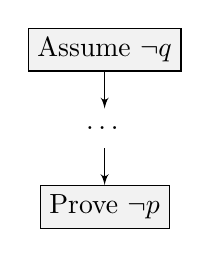
\begin{tikzpicture}
\node [block] (assume-p) at (0,0) {Assume $\neg q$};
\path [line] (assume-p) -- (0,-.75);
\node at (0,-1) {$\dots$};
\node [block] (q) at (0,-2) {Prove $\neg p$};
\path [line] (0,-1.25) -- (q);
\end{tikzpicture}
\end{center}
\end{bmethod}


\begin{theorem}\label{theorem:s2-even-s-even}
For all $s \in \mathbb{Z}$, if $s^2$ is even, then $s$ is even.
\end{theorem}
To start a proof, we would write ``Let $s \in \mathbb{Z}$ be arbitrary.'' Then we would need to prove if $s^2$ is even, then $s$ is even. Our usual way of proving this would be to suppose that $s^2$ is even. So, there would exist an integer $k$ such that $s^2=2k$. But then how would we ever express $s$? It seems awkward to square root both sides and have $s=\pm\sqrt{2k}$. Where would we go from here? It appears that a direct proof of the implication is awkward. Let us try an indirect proof (with the selection of $s \in \mathbb{Z}$ still arbitrary). Before starting the proof, recall from Section~\ref{section:examples-of-assumed-propositions} that an integer that is not odd is even, and that an integer that is not even is odd.
\begin{proof}
Let $s \in \mathbb{Z}$ be arbitrary. We wish to show that if $s^2$ is even, then $s$ is even. To prove this, suppose $s$ is not even. Then, due to Section~\ref{section:examples-of-assumed-propositions}, $s$ is odd. We wish to prove that $s^2$ is odd. Since $s$ is odd, there exists an integer $a$ such that $s=2a+1$. Let $b = 2a^2+2a$. Then $b$ is an integer, and $s^2=(2a+1)^2=4a^2+4a+1=2(2a^2+2a)+1=2b+1$. Since $s^2=2b+1$ and $b$ is an integer, $s^2$ is odd. 
\end{proof}

If you need to prove an implication, always try a direct proof\index{direct proof}. However, if you get stuck in a direct proof, consider proving the contrapositive of the implication instead (which is called the \defn{indirect proof}\index{indirect proof}).

\begin{exercise}
Prove: for all $k \in \mathbb{Z}$, if $k^2$ is odd, then $k$ is odd.
\end{exercise}

\begin{bwarning}{}{dont-assume-q-indirect}
Notice that to prove $p \to q$ using the indirect method, we end up assuming $\neg q$. We \emph{never} assume $q$. (That is, never assume what you need to prove.)
\end{bwarning}

\section{Proof by contradiction}\label{section:proof-by-contradiction}

There are situations where the usual proof techniques do not lead to the required propositions. A new method -- proof by contradiction\index{contradiction}\index{proof by contradiction} -- offers another opportunity to prove certain statements by allowing the proof writer to add an additional assumption.

Suppose that we need to prove $q$. If we feel that we are stuck having used all the propositions we were allowed to assume, we might add a new assumption, namely $\neg q$.
\begin{bmethod}{Prove $q$ by contradiction}{contradiction-general}
\begin{center}
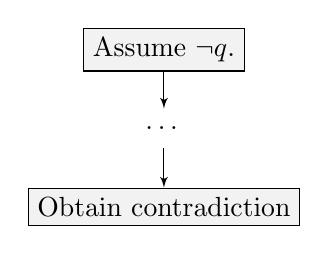
\begin{tikzpicture}
\node [block] (assume-p) at (0,0) {Assume $\neg q$.};
\path [line] (assume-p) -- (0,-.75);
\node at (0,-1) {$\dots$};
\node [block] (q) at (0,-2) {Obtain contradiction};
\path [line] (0,-1.25) -- (q);
\end{tikzpicture}
\end{center}
\end{bmethod}
By adding $\neg q$, if we can obtain a contradiction, then it must have been erroneous to assume $\neg q$, so we could conclude that $q$ is true. In other words, due to having a contradiction, we would then conclude that our original assumption of $\neg q$ must have been false, which means that $q$ is true.

\begin{theorem}
The real number $\sqrt{2}$ is irrational.
\end{theorem}
Recall that a real number $r$ is rational if there exists an integer $b$ and a non-zero integer $c$ such that $r = \frac{b}{c}$. In the proof we look at below, we will even look at the stronger situation where $\frac{b}{c}$ is reduced as much as possible. So, for instance, if $r$ is $\frac{4}{12}$, we would need to reduce the fraction to $\frac13$. Note that, once $r=\frac{4}{12}$ is reduced, then $b=1$ and $c=3$ do not share any common prime factors.
\begin{proof}
In order to obtain a contradiction, suppose that $\sqrt{2}$ is rational. Then, there exists an integer $b$ and a non-zero integer $c$ such that $\sqrt{2} = \frac{b}{c}$, and we consider the situation where $\frac{b}{c}$ is reduced, so that $b$ and $c$ do not share any common factors greater than $1$.

Since $\sqrt{2} = \frac{b}{c}$, we have $c\sqrt{2}=b$ by multiplication, and $2c^2=b^2$ by squaring. But since $b^2=2(c^2)$ proves that $b^2$ is even, by  Theorem~\ref{theorem:s2-even-s-even}, $b$ is even. Since $b$ is even, there exists an integer $k$ such that $b=2k$. Then $2c^2=(2k)^2$, so $2c^2=4k^2$, and by division, $c^2=2(k^2)$. Since $c^2$ is even, $c$ is even by Theorem~\ref{theorem:s2-even-s-even}.

But if $b$ and $c$ are both even, then they share common factors greater than $1$, contradicting the earlier statement that $b$ and $c$ do not share any common factors greater than $1$. Our original assumption that $\sqrt{2}$ is rational must have been incorrect: therefore, $\sqrt{2}$ is irrational.
\end{proof}
\begin{bwarning}{}{dont-assume-q-general-contradiction}
To prove $q$ by contradiction, note that we do not assume $q$ is true. Rather, we assume that $\neg q$ is true then work towards obtaining a contradiction.
\end{bwarning}

Now, we examine a special case of proof by contradiction. The method we are about to describe is just a special case of the general proof by contradiction that we have already described, but it occurs so frequently that we write extensively about this special case.

Suppose that we need to prove the implication $p \to q$. Following the method of direct proof, we would assume $p$. Then, we would need to prove $q$. However, if we feel that we are getting nowhere in proving $q$, we can prove $q$ by contradiction. Following the method already mentioned, we would assume $\neg q$, then work to obtain a contradiction. In other words, to prove $p \to q$ by contradiction, we assume two propositions: first, we assume $p$, and then we assume $\neg q$. Then, once we obtain a contradiction, we would then conclude that, our assumption of $\neg q$ must have been false.
\begin{bmethod}{Proving $p \to q$ by contradiction}{pimpliesq-contradiction}
\begin{center}
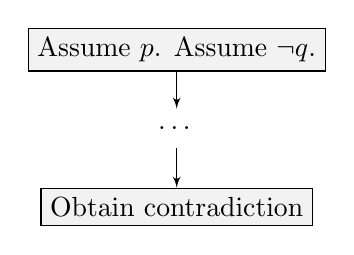
\begin{tikzpicture}
\node [block] (assume-p) at (0,0) {Assume $p$. Assume $\neg q$.};
\path [line] (assume-p) -- (0,-.75);
\node at (0,-1) {$\dots$};
\node [block] (q) at (0,-2) {Obtain contradiction};
\path [line] (0,-1.25) -- (q);
\end{tikzpicture}
\end{center}
\end{bmethod}
\begin{bwarning}{}{dont-assume-q-implication}
Notice that to prove $p \to q$ by contradiction, we end up assuming $\neg q$. We \emph{never} assume $q$. (That is, never assume what you need to prove.) This mirrors the warnings mentioned as Warning~\ref{warning:dont-assume-q-indirect} and Warning~\ref{warning:dont-assume-q-general-contradiction}. In this warning as in the previous two warnings, we never assume the proposition $q$.
\end{bwarning}

As an example, let us visit the game of Minesweeper. A typical cell (those found in the middle of the Minesweeper board) is surrounded by 8 other cells. (The cells on the edge are surrounded by only five other cells, while the four corner cells are surrounded by only three other cells.) The ``raised'' cells are unknowns. The more ``indented'' cells are known. (Indented cells without a number are zeros: none of the 8 surrounding cells are mines.) The cells which have a red triangular flag are marked by the game player (usually by right-clicking) to indicate that these are mines.

To carefully understand, let us consider the example in Figure~\ref{figure:minesweeper01}. The cell labeled 2 to the right of Cell Y should have two mines. The cell to the upper right (with a 2), the cell to the right (with a 1), the cell to the lower right (blank, so a zero), and the cell below (the 1 to the right of Z) have all been cleared. The cell above the 2 is already marked as a mine. While that spot is ``technically not known", the person playing felt confident enough to mark that spot a mine. In addition, Cell X, Cell Y, and Cell Z are unknowns. For an example of the language of proof that can be used, let us consider the same example. The cell labeled 2 to the right of Cell Y should have two mines. Since there is already one marked mine, among the three cells Cell X, Cell Y, and Cell Z, exactly one of these is a mine.

\begin{figure}[hbt]
\begin{center}
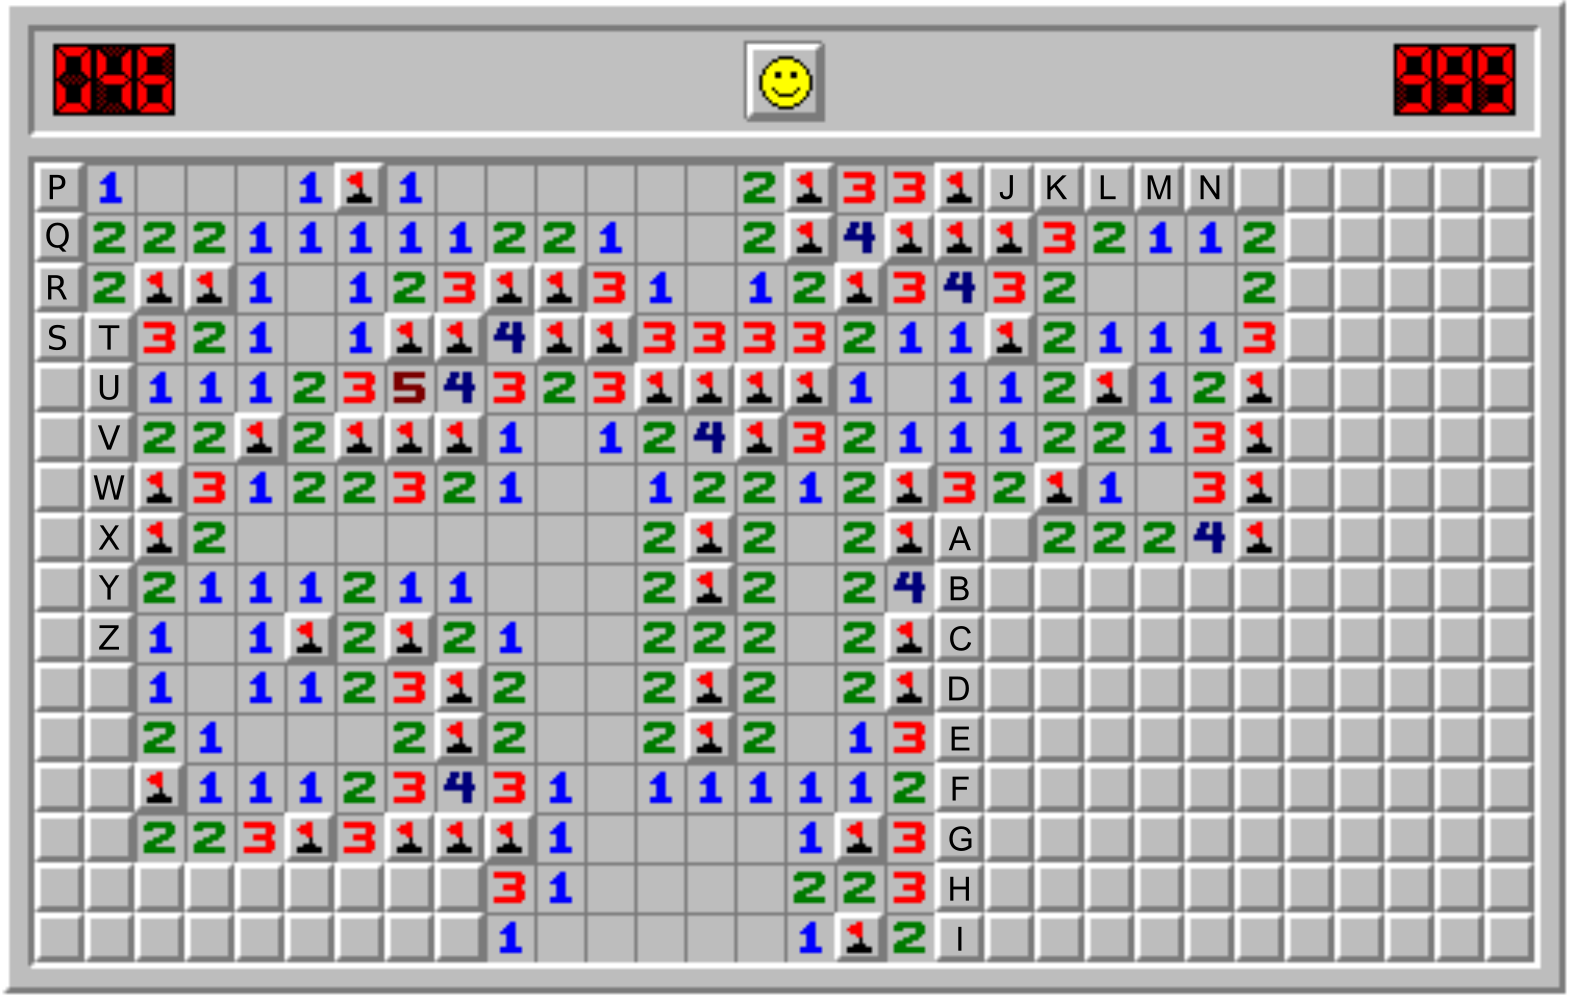
\includegraphics[width=0.78\textwidth]{minesweeper01}
\end{center}
\caption{A player who is ``stuck'' in Minesweeper}\label{figure:minesweeper01}
\end{figure}

The game of Minesweeper gives us a fun way to examine proving $p \rightarrow q$ by contradiction. How would one prove the statement ``If the Minesweeper configuration is as given in Figure~\ref{figure:minesweeper01}, then Cell I is safe'' by contradiction? Following Method~\ref{method:pimpliesq-contradiction}, we should first assume we have the mine configuration given in Figure~\ref{figure:minesweeper01}. Then, to prove that Cell I is safe by contradiction, we assume that Cell I is not safe -- in other words, we assume that Cell I is a mine.
\begin{theorem}
If the Minesweeper configuration is as given in Figure~\ref{figure:minesweeper01}, then Cell I is safe.
\end{theorem}
\begin{proof}
Suppose we have the given mine configuration from Figure~\ref{figure:minesweeper01}. To obtain a contradiction, suppose that Cell I is a mine. Then the 3 to the left of H has all of its mines so, Cell H and Cell G are both safe. Then the 3 to the left of G has one discovered mine, and one possible mine at F, leaving only at most two neighboring mines to a cell labeled with 3, a contradiction.
\end{proof}
In the previous proof, the contradiction obtained is that both ``F has only two neighboring mines'' and ``F has exactly three neighboring mines'' cannot both be true.

%NEXTEDITION: include every possible minesweeper proof that I can think of

\begin{theorem}\label{theorem:minesweeper01-V-safe-contradiction}
If the Minesweeper configuration is as given in Figure~\ref{figure:minesweeper01}, then Cell V is safe.
\end{theorem}
\begin{proof}
Suppose we have the given mine configuration from Figure~\ref{figure:minesweeper01}. In order to obtain a contradiction, assume that Cell V is a mine. Then because the cell labeled 1 to the right of U already has its 1 mine at V, the cells T and U must be safe. Then, the cell labeled 3 to the right of Cell T only has the two-previously discovered mines, and since the T and U are not mines, the 3 is not satisfied, a contradiction.
\end{proof}

\begin{exercise}
Prove by contradiction: If the Minesweeper configuration is as given in Figure~\ref{figure:minesweeper02}, then Cell B is safe.
\end{exercise}
\begin{figure}[hbt]
\begin{center}
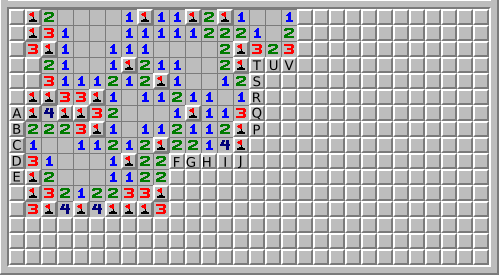
\includegraphics[width=0.78\textwidth]{minesweeper02}
\end{center}
\caption{A player who is ``stuck'' in Minesweeper}\label{figure:minesweeper02}
\end{figure}

When proving $p \to q$ by contradiction, you first assume $p$, and then because you want to prove $q$ by contradiction, you assume $\neg q$. There are three ways that proving $p \to q$ may end:
\begin{itemize}
\item You end up with $\neg p$ which means you end up with the contradiction $p \wedge \neg p$. Typically, though not always, a proof of this kind can be restructured to an indirect proof of $p \to q$ which avoids a proof by contradiction.
\item You end up with $q$, which means you end up with the contradiction $q \wedge \neg q$. These typically feel bizarre, because you assumed $\neg q$ and you somehow used $p$ and $\neg q$ to obtain $q$.
\item You end up with $r \wedge \neg r$, for some proposition $r$ which is different from $p$ and different from $q$.
\end{itemize}


\section{Proof by cases}\label{section:proof-by-cases}

In the last section, we saw the method of proof by contradiction as one way forward when it seems like we are stuck in a proof. Another method that is useful in such ``sticky'' situations is a proof by cases.

Suppose that one wishes to prove $p \rightarrow q$. The natural method is to assume $p$ first, then attempt to prove $q$. However, if you get stuck proving $q$, you might try to identify $k$ propositions, which we will name $h_1,h_2,\dots,h_k$, where $k \geq 2$. Typically, $k$ should be small: perhaps no more than $5$, ideally. The goal is to have propositions  $h_1,h_2,\dots,h_k$ where the following can be proved:
\begin{itemize}
\item $p \rightarrow (h_1 \vee h_2 \vee \dots \vee h_k)$
\item $h_1 \rightarrow q$
\item $h_2 \rightarrow q$
\item $h_3 \rightarrow q$
\item and so on until
\item $h_k \rightarrow q$
\end{itemize}
If all the proofs above are successful, then one can validly conclude that $q$ is true.

Why does this work? The proof of $p \rightarrow (h_1 \vee h_2 \vee \dots \vee h_k)$ is the identification of the cases. For simplicity, let us consider a situation where $k=3$. That is, let us examine $p \rightarrow (h_1 \vee h_2 \vee h_3)$. This is saying that from $p$, one of three things must occur: either $h_1$ must be true, or $h_2$ must be true, or $h_3$ must be true. At least one of these three propositions must be true. In other words, we want to ensure that it is inevitable that at least one of $h_1$ or $h_2$ or $h_3$ are true. Then, no matter which of these three things are true, we will reach our destination. If $h_1$ is true, then we get to apply the proof that we present of $h_1 \rightarrow q$. If instead $h_2$ is true, then we apply the proof of $h_2 \rightarrow q$. If $h_3$ is true, then we apply the proof of $h_3 \rightarrow q$. Here we saw an example of $k=3$, which is a proof in three cases.

For a proof in four cases ($k=4$), we must identify four propositions $h_1,h_2,h_3,h_4$. The proof's author should first argue that $p \rightarrow (h_1 \vee h_2 \vee \vee h_3 \vee h_4)$ is true. Then there are four additional proofs to do, namely $h_1 \rightarrow q$ and $h_2 \rightarrow q$ and $h_3 \rightarrow q$ and $h_4 \rightarrow q$.

Let us consider the following example:
\begin{theorem}
If the Minesweeper configuration is as given in Figure~\ref{figure:minesweeper01}, then Cell N is safe.
\end{theorem}
\begin{proof}
Assume we have the given mine configuration from Figure~\ref{figure:minesweeper01}.
Because of the 3 below K, of the three cells J, K, and L, exactly two must be mines. That is, either J and K are mines with L safe, or J and L are mines with K safe, or K and L are mines with J safe. We break into three cases:
\begin{itemize}
\item If Cell J and Cell K are mines and Cell L is safe, then Cell M must be a mine so that the $2$ below Cell L has its second mine. Then the $1$ below Cell M has all its mines discovered, so Cell M is safe and Cell N is safe.
\item If Cell J and Cell L are mines and Cell K is safe, then because of the 2 under Cell L, Cell M must be a mine. However, this case is impossible because the 1 below M is surrounded by mines at both Cell L and Cell M.
\item If Cell K and Cell L are mines and Cell J is safe, then the 1 under Cell M has its mine located at Cell L, so Cell M and Cell N are both safe.
\end{itemize}
No matter which of the three cases occur, we can see that Cell N is safe.
\end{proof}
In this example, $k=3$. Note that ``we have the given mine configuration from Figure~\ref{figure:minesweeper01}'' is $p$, following the notation from earlier. Let us identify the three situations:
\begin{itemize}
\item $h_1$ is ``J and K are mines with L safe''
\item $h_2$ is ``J and L are mines with K safe''
\item $h_3$ is ``K and L are mines with J safe''
\end{itemize}
and our proof of $p \rightarrow (h_1 \vee h_2 \vee h_3)$ is embedded in the short sentence, ``Because of the 3 below K, of the three cells J, K, and L, exactly two must be mines.'' In the proof, after the sentence ``We break into three cases'' we have presented proofs of $h_1 \rightarrow q$ and $h_2 \rightarrow q$ and $h_3 \rightarrow q$. No matter what, we reach the conclusion of $q$, where $q$ is namely ``Cell N is safe.'' (One word about the second case, where K was assumed safe: it turned out that this was impossible, so while it seemed that we had three cases in the beginning, in retrospect, we only had two cases.)

The idea of proof by cases is to branch out from the situation of $p$ and look at one of a number ($h_1,\dots,h_k$) situations, at least one of which \emph{must} hold. Then, assuming each of these situations, we either determine that the situation was actually impossible (as we had in our second case above) or that we reach the conclusion that $q$ is true (as we did in cases one and three above).

Let us revisit Theorem~\ref{theorem:minesweeper01-V-safe-contradiction}, which we earlier proved by contradiction, and now provide a proof of the same theorem by cases. In this proof by cases, the proof of the first case is an embedded proof by cases.
\begin{theorem}
If the Minesweeper configuration is as given in Figure~\ref{figure:minesweeper01}, then Cell V is safe.
\end{theorem}
\begin{proof}
Suppose we have the given mine configuration from Figure~\ref{figure:minesweeper01}.
Because of the $1$ in row $1$ column $2$, either Cell P is a mine or Cell Q is a mine. We proceed by cases.
\begin{itemize}
\item In the first case, P is a mine. So Q is safe. Since P is a mine, the 2 in $(2,2)$ has all necessary mines, so R is safe. Then exactly one of S or T is a mine, due to the 2 in $(3,2)$. We proceed in two subcases:
\begin{itemize}
\item If S is a mine and T is safe, then U must be a mine for the third mine of the 3 located at $(4,3)$. Since the 1 to the right of U has all its mines, V must be safe.
\item If T is a mine and S is safe, then U is safe because the 3 located at $(4,3)$ has all its mines.  In addition, the 1 to the right of U already has its mine at T, so V is safe.
\end{itemize}
In both subcases V is safe.
\item In the second case, Q is a mine, so P is safe. Since Q is a mine, the 2 in $(3,2)$ has all necessary mines, so R, S, and T are all safe. Since T is safe, due to the 3, U is a mine. Since the 1 to the right of U has all its mines, V is safe.
\end{itemize}
In both cases, V is safe.
\end{proof}
Let us analyze the structure of this proof and see how it fits our framework. Following our notation from earlier, we have an initial hypothesis $p$ that ``we have the given mine configuration from Figure~\ref{figure:minesweeper01}'' and then identified two propositions, where $h_1$ was ``Cell P is a mine'' and $h_2$ was ``Cell Q is a mine.'' Our proof of $p \rightarrow (h_1 \vee h_2)$ is given in the sentence ``Because of the $1$ in row $1$ column $2$, either Cell P is a mine or Cell Q is a mine.''

After the sentence ``We proceed by cases'' in the proof above, the proof presented a proof of $h_1 \rightarrow q$ and a proof of $h_2 \rightarrow q$, where $q$ was ``Cell V is safe.'' We postpone the discussion of the proof of $h_1 \rightarrow q$ momentarily. The proof of $h_2 \rightarrow q$ was the text that started with ``In the second case, Q is a mine, ...'' and ended with ``Since the 1 to the right of U has all its mines, V is safe.''

What about the proof of $h_1 \rightarrow q$? We proved this by cases. Here, the initial hypothesis was ``P is a mine'', though we may of course use our earlier initial hypothesis $p$ as well, which is how we immediately obtained the next sentence ``So Q is safe,'' and further along obtained the fact that R is safe as well. Within the proof, we identified two possible situations: let us call $i_1$ the situation of ``S is a mine an T is safe'' and call $i_2$ the situation ``T is a mine and S is safe.'' The proof that the initial hypothesis implies $(i_1 \vee i_2)$ is proved in the sentence ``Then exactly one of S or T is a mine, due to the 2 in $(3,2)$.'' The inner-indented items provide the proof of $i_1$ implies that V is safe and the proof of $i_2$ implies that V is safe.

\begin{bwarning}{The error of missing cases}{}
When proving by cases, it is important to state the case hypotheses $h_1,\dots,h_k$. It is important to explain why at least one case hypothesis holds. (That is, be sure to include an argument -- often very short -- that $p \rightarrow (h_1 \vee \dots \vee h_k)$ is true.) Otherwise, you run into the situation of having missing cases.
\end{bwarning}
When initially starting, you might identify propositions $h_1$, $h_2$, and $h_3$. However, if you have trouble proving $p \rightarrow (h_1 \vee h_2 \vee h_3)$, it might be because $p \rightarrow (h_1 \vee h_2 \vee h_3)$ is not true. Perhaps there is a ``missing case.'' Sometimes, by keeping $h_1$,$h_2$, and $h_3$ exactly as you thought of them, but also identifying a new proposition $h_4$, it is possible to prove $p \rightarrow (h_1 \vee h_2 \vee h_3 \vee h_4)$. When it is time to write your formal proof, imagine the immediately before writing ``We proceed in cases'' you would write the sentence ``Either $h_1$ or $h_2$ or $h_3$ or $h_4$.'' You want the reader of your proof to be convinced that ``Either $h_1$ or $h_2$ or $h_3$ or $h_4$'' is true.

\begin{bwarning}{The error of not reaching the required conclusion}{}
If you have $k$ cases, beyond the proof of $p \rightarrow (h_1 \vee \dots \vee h_k)$, be sure to provide the $k$ proofs of the form $h_j \rightarrow q$. In particular, be sure to reach the conclusion $q$ in each case.
\end{bwarning}

\begin{exercise}
Prove by cases: If the Minesweeper configuration is as given in Figure~\ref{figure:minesweeper02}, then Cell V is a mine. (While it is possible to provide a proof by contradiction, it would  be good to practice proof by cases. As a hint, start where Cell P, Cell Q, and Cell R are, and create the three cases. Note that one of the cases will be impossible, but there will still be the remaining cases to consider.)
\end{exercise}

\begin{exercise}
Prove: If the Minesweeper configuration is as given in Figure~\ref{figure:minesweeper02}, then Cell F is a mine.
\end{exercise}

We started this chapter by discussing how one uses a conjunction, but did not discuss using a disjunction. Often, using a disjunction fits the pattern of a proof by cases. Some details are provided in the next section.


\section{Proving/using disjunctions}

To use $p \vee q$, if we knew $p \vee q$ and we knew $\neg p$, then we can conclude $q$. More generally, if we know $p_1 \vee p_2 \vee p_3$ and we knew $\neg p_1$ and we know $\neg p_2$, then we can conclude $p_3$.

Often, we use a disjunction in a way that essentially follows a proof by cases, because we are often in the situation of needing to prove the implication $(p_1 \vee p_2 \vee \dots \vee p_k) \rightarrow q$. Of course, we'd immediately assume $(p_1 \vee \dots \vee p_k)$. Then if we prove $p_1 \rightarrow q$ and prove $p_2 \rightarrow q$ and so on, all the way up to proving $p_k \rightarrow q$, then we can conclude $q$ by cases, completing our proof of $(p_1 \vee p_2 \vee \dots \vee p_k) \rightarrow q$.

Suppose we had to prove the disjunction $p \vee q$. Of course, if we knew $p$ was true, we can conclude $p \vee q$.
\begin{center}
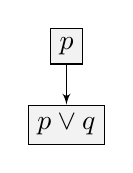
\begin{tikzpicture}
\node [block] (assume-p) at (0,0) {$p$};
\node [block] (q) at (0,-1) {$p \vee q$};
\path [line] (assume-p) -- (q);
\end{tikzpicture}
\end{center}
Likewise, if we knew $q$ was true, we can conclude $p \vee q$.

Typically, a bit more may be needed to prove $p \vee q$. To prove $p \vee q$, one can add in the assumption of $\neg p$ and then attempt to prove $q$. Alternately, one can add in the assumption of $\neg q$ and then attempt to prove $p$. If one approaches a proof of  $p \vee q$ by adding in the assumption of $\neg p$, this can be thought of as a proof by cases: either $p$ or $\neg p$. If $p$ holds, then $p \vee q$ is automatic. If $\neg p$ holds, then the provided proof of $(\neg p) \rightarrow q$ is the proof of the second case.

\section{Proving/using biconditionals}

Suppose you need to prove the biconditional $p \leftrightarrow q$. Since $p \leftrightarrow q$ is logically equivalent to $(p \rightarrow q) \wedge (q \rightarrow p)$, one can leave proving $p \leftrightarrow q$ to proving $p \rightarrow q$ and proving $q \rightarrow p$. The proof of $p \rightarrow q$ is often informally called the \defn{forward direction} with the proof of $q \rightarrow p$ called the \defn{reverse direction}. Of course, either or both implications can be proved by considering the contrapositive instead. That is, here are four possible methods for proving $p \leftrightarrow q$.
\begin{itemize}

\item
Directly prove $p \rightarrow q$. That is, assume $p$, then prove $q$.
Then, directly prove $q \rightarrow p$. That is, assume $q$, then prove $p$.

\item
Directly prove $p \rightarrow q$. That is, assume $p$, then prove $q$.
Then, indirectly prove $q \rightarrow p$. That is, assume $\neg p$, then prove $\neg q$.

\item
Indirectly prove $p \rightarrow q$. That is, assume $\neg q$, then prove $\neg p$.
Then, directly prove $q \rightarrow p$. That is, assume $q$, then prove $p$.

\item
Indirectly prove $p \rightarrow q$. That is, assume $\neg q$, then prove $\neg p$.
Then, indirectly prove $q \rightarrow p$. That is, assume $\neg p$, then prove $\neg q$.

%Directly prove $p \rightarrow q$. That is, assume $p$, then prove $q$.
%Indirectly prove $p \rightarrow q$. That is, assume $\neg q$, then prove $\neg p$.
%
%Then, indirectly prove $q \rightarrow p$. That is, assume $\neg p$, then prove $\neg q$.
%Then, directly prove $q \rightarrow p$. That is, assume $q$, then prove $p$.
\end{itemize}% Proving iff: the forward and the contrapositive of the reverse
To use $p \leftrightarrow q$, we again appeal to its logical equivalence to $(p \rightarrow q) \wedge (q \rightarrow p)$. Thus,
\begin{itemize}
\item Knowing $p \leftrightarrow q$ and knowing $p$ means we can conclude $q$.
\item Knowing $p \leftrightarrow q$ and knowing $q$ means we can conclude $p$.
\item Knowing $p \leftrightarrow q$ and knowing $\neg p$ means we can conclude $\neg q$.
\item Knowing $p \leftrightarrow q$ and knowing $\neg q$ means we can conclude $\neg p$.
\end{itemize}
%
There is a generalization of $p \leftrightarrow q$. One might read a theorem whose statement says
``\defn{the following are equivalent} \index{the following are equivalent} (TFAE)\index{TFAE}
\begin{itemize}
\item $a$
\item $b$
\item $c$
\item $d$''
\end{itemize}
where $a$, $b$, $c$, and $d$ are all propositions. This is taken to mean that
$a \leftrightarrow b$, and
$a \leftrightarrow c$, and
$a \leftrightarrow d$, and
$b \leftrightarrow c$, and
$b \leftrightarrow d$, and
$c \leftrightarrow d$.

There are many ways to prove such a statement. For example, one can prove $a \rightarrow b$ and prove $b \rightarrow c$ and prove $c \rightarrow d$ and prove $d \rightarrow a$. Alternately, one can prove $a \rightarrow b$ and prove $b \rightarrow c$ and prove $c \rightarrow a$ and prove $a \rightarrow d$ and prove $d \rightarrow a$. Here are diagrams that show both of these major proof outlines:

\begin{center}
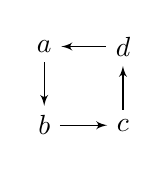
\begin{tikzpicture}
\node (a) at (0,0) {$a$};
\node (b) at (0,-1) {$b$};
\node (c) at (1,-1) {$c$};
\node (d) at (1,0) {$d$};
\path [line] (a) -- (b);
\path [line] (b) -- (c);
\path [line] (c) -- (d);
\path [line] (d) -- (a);
\end{tikzpicture}
\quad\quad\quad
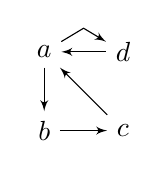
\begin{tikzpicture}
\node (a) at (0,0) {$a$};
\node (b) at (0,-1) {$b$};
\node (c) at (1,-1) {$c$};
\node (d) at (1,0) {$d$};
\path [line] (a) -- (b);
\path [line] (b) -- (c);
\path [line] (c) -- (a);
\path [line] (d) -- (a);
\path [line] (a) -- (0.5,0.3) -- (d);
\end{tikzpicture}
\end{center}
These are schematic diagrams of proof outlines. As long as one can go from any proposition to any other proposition along a directed arrow, then a proof of a ``the following are equivalent'' statement is complete.

Suppose you knew that $a$, $b$, $c$ and $d$ were all equivalent. (An example is the Invertible Matrix Theorem from linear algebra.) Then, if you also knew $b$, you could conclude $c$. If you know $d$, you could conclude $a$. If you knew $\neg c$, you could conclude $\neg d$, and so on.

\subsection{A characterization is not a substitute for a definition}

Recall Definition~\ref{definition:odd}, that an integer $b$ is odd if there exists an integer $s$ such that $b=2k+1$. As a nice review problem, prove the following theorem:
\begin{theorem}\label{theorem:odd-characterization}
Let $b$ be an integer. Then $b$ is odd if and only if there exists an integer $u$ such that $b=2u-1$.
\end{theorem}
Theorem~\ref{theorem:odd-characterization} is known as a \defn{characterization}\index{characterization} of being odd. However, when asked to state the definition of odd, it would be incorrect to write ``an integer $b$ is odd if there exists an integer $u$ such that $b=2u-1$'' as the definition.

Why not? Well, this is really a form of circular thinking. The definition (the original definition) needs to be referenced in proving Theorem~\ref{theorem:odd-characterization} in the first place. Even after Theorem~\ref{theorem:odd-characterization} is proved, the text of the definition should remain as it was, and should not be changed just because we have now proved Theorem~\ref{theorem:odd-characterization}. This principle applies in general:
\begin{bwarning}{}{}
After a characterization is known (through proof, or accepted as true for free), do not replace the definition with text from the characterization theorem.
\end{bwarning}

\section{Uniqueness}\label{section:uniqueness}

Suppose $U$ is a set and $P(x)$ is a predicate. There are times when we will need to prove ``There exists a unique $b \in U$ such that $P(b)$.'' (Notice the inclusion of the new word ``unique'' here.) How does one prove \defn{uniqueness}\index{uniqueness}? Or more generally, how does one prove existence and uniqueness? The sentence in quotes is sometimes denoted by including an exclamation point as in: $\exists ! b \in U\,[P(b)]$.
\begin{example}
We revisit Example~\ref{example:universal-city}. There exists a unique resident $x$ of Uruapan whose blood type is O+. (Namely, Finley is the only resident of Uruapan with blood type O+.)
\end{example}

How one should prove this is informed by how we can rewrite $\exists ! b \in U\,[P(b)]$ in terms of earlier symbols. In fact, $\exists ! b \in U\,[P(b)]$ is logically equivalent to $[\exists b \in U\,[P(b)]] \wedge [\forall a \in U \forall c \in U [(P(a) \wedge P(c)) \rightarrow (a=c)]]$. The portion after the $\wedge$ symbol is the unique part. Thus,
\begin{bmethod}{}{proving-uniqueness}
To prove that $x$ satisfying $P(x)$ is unique, suppose $a$ satisfies $P(a)$, and suppose $c$ satisfies $P(c)$. Then prove $a=c$.
\end{bmethod}

\begin{example}
Suppose we need to prove ``A mayor of Proofville is unique.'' A proof could start by writing the sentence ``Let $a$ be a mayor of Proofville.'' The following sentence could be ``Let $c$ be a mayor of Proofville.'' Then, the proof author should work towards proving $a=c$.
\end{example}
Even in this example, it is ideal to just write ``Let $a$ be a mayor of Proofville Let $c$ be a mayor of Proofville.'' in two consecutive sentences instead of trying to combine these into one sentence. The point is that after these two sentences are written, the proof writer is not saying that $a$ and $c$ are different, and the proof writer is also not saying that $a$ and $c$ are the same. Without assuming (even implicitly in how it is written) that $a=c$ or that $a\not=c$, it is much easier to then lead the reader to the eventual conclusion that $a=c$. (Imagine that it is more problematic to go towards the conclusion of $a=c$ if one has the erroneous sentence ``Let $a$ and $c$ be different mayors of Proofville'' at the beginning of the proof.)

\begin{theorem}
There exists a unique real number $b$ such that $2b+7=1$.
\end{theorem}
\begin{proof}
To prove existence, let $b=-3$. Then $2b+7=2(-3)+7=-6+7=1$. To prove uniqueness, suppose that $a$ satisfies $2a+7=1$, and suppose that $c$ satisfies $2c+7=1$. (At this point in the proof, we are not saying that $a=c$. We are also not saying that $a \not= c$ for that matter.) Then, by transitivity of equality, $2a+7=2c+7$. By subtraction on both sides, $2a=2c$. By division, $a=c$, so uniqueness is proved.
\end{proof}
By contrast, it would be impossible to prove that there exists a unique real number $b$ such that $b^2-3b=40$. Existence is true (see Theorem~\ref{theorem:existence-not-uniqueness}), but uniqueness is not true. (This is because $a=-5$ is a solution to $x^2-3x=40$ and $c=8$ is also a solution to $x^2-3x=40$.)

\begin{remark}
In English, ``a'' and ``and'' are indefinite articles, while ``the'' is the only definite article. An indefinite article is used when there is possibly uncertainly regarding how many objects there are, or if there is known to be only one, emphasizing that there's only one is unimportant. (Example: Here is an apple.) The word ``the'' is used the communicate that there's only one of a certain object. (Example: This is the [only] apple in the store.)

Now that we have discussed uniqueness, challenge yourself to pay attention to how mathematicians speak and write when using articles. While the use of definite versus indefinite articles is often a matter of taste for most definitions, you will begin to notice that the word ``the'' only makes certain appearances (especially in certain theorems and definitions) only after a uniqueness statement is proved.
\end{remark}

\section{Connection to the past: examples from previous classes}\label{section:previous-class-proofs}

Your previous math classes have offered small examples of many of the methods presented in the previous sections of this chapter:
\begin{itemize}

\item In algebra, you used the implication ``If $a=b$ then $a+c=b+c$.'' Actually, a more complete version of this has quantifiers: you used ``For all reals $a$, $b$, and $c$, if $a=b$, then $a+c=b+c$.'' This procedure was called ``adding $c$ to both sides'' in your algebra class. In fact, when you were asked to solve the equation $x-5=4$, the idea that $x$ was real was implied. To use the quantified statement (following Method~\ref{method:using-forall}, we'd consider $x-5$ to be the real $a$, have $b=4$, then use $c=5$. Then, since we have $a=b$ which is specifically $x-5=4$ for us, we could apply modus ponens (following Method~\ref{method:modus-ponens}) to get $a+c=b+c$ which in this example is $(x-5)+5=4+5$, and we are now well on our way to solving for $x$.

\item Actually, a more complete statement is ``For all reals $a$, $b$, and $c$, we have $a=b$ if and only if $a+c=b+c$.'' The biconditional shows that adding $c$ to both sides is reversible. In contrast, ``For all reals $a$ and $b$, if $a=b$, then $a^2=b^2$'' is true, but trying to change the implication to a biconditional will not work. (It is possible to have $a^2=b^2$ with $a \not= b$.) This is why, when solving equations such as $\sqrt{x-3}=10$ which requires squaring both sides, students are admonished to check their solutions, because not every ``algebra move'' they apply is reversible.

\item Also from algebra, the statement ``For all reals $a$ and $b$, if $ab=0$, then $a=0$ or $b=0$'' known as the Zero Product Property is used to solve an equation such as $x^2-x-6=0$, by first writing $(x-3)(x+2)=0$ and applying the statement using $a=x-3$ and $b=x+2$.

\item As a general comment, nearly all properties from algebra such as $a(b+c)=ab+ac$ which are used frequently by an algebra student actually come with universal quantifiers.

\item In precalculus, verifying a trigonometric identity often involves using other trigonometric identities. Some trig identities get \emph{used} in the process of \emph{proving} one new trig identity.

%\item Two-sided characterization in terms of one-sided limits

\item In calculus, given a function $f$, students may be asked to prove that the function $f$ is continuous at the $x$-value $6$. This is typically done by verifying the three-part definition of continuity, an example of following Method~\ref{method:proving-borogove}.

\item In calculus, students may be asked to show that a given function $f$ has a limit of $L$ as $x$ approaches a given number $c$ using the precise $\varepsilon$-$\delta$ definition of limit, which states the limit of the function $f$ as $x$ approaches $c$ is $L$ if for all $\varepsilon > 0$, there exists $\delta > 0$ such that if $0<|x-c|<\delta$, then $|f(x)-L|<\varepsilon$. In the process of verifying that the definition holds following Method~\ref{method:proving-borogove}, one ends up proving a universally-quantified statement, proving a (smaller) existentially-quantified statement, and (eventually) proving an implication.

\item From calculus, the Squeeze Theorem states that if $\displaystyle \lim_{x \to c} f(x) = L$ and $\displaystyle \lim_{x \to c} h(x) = L$ and $f(x) \leq g(x) \leq h(x)$ for all $x$, then $\displaystyle \lim_{x \to c} g(x) =L$. To use the Squeeze Theorem, after verifying that the three requirements hold, the student applies modus ponens with the Squeeze Theorem to conclude a limit value for the function $g$.

\item From calculus, the Intermediate Value Theorem states that if $f$ is a function that is continuous on the interval $[a,b]$, then for all $y$ between $f(a)$ and $f(b)$, there exists $c$ in the interval $[a,b]$ such that $f(c)=y$. Students in calculus use this theorem by first verifying the given function $f$ is continuous on $[a,b]$. By modus ponens, a universally-quantified statement is true. After selecting (writer's choice) any $y$-value between $f(a)$ and $f(b)$, this universally-quantified statement is used following Method~\ref{method:using-forall}.

\item From calculus, Rolle's Theorem states that if $f$ is continuous on the interval $[a,b]$ and differentiable on the interval $(a,b)$ and $f(a)=f(b)$, then there exists $c$ in the interval $(a,b)$ such that $f'(c)=0$. To use Rolle's Theorem, students in calculus verify that a given function $f$ is continuous on $[a,b]$ and is differentiable on $(a,b)$ and that $f(a)$ equals $f(b)$. Then modus ponens allows the student to conclude that there exists $c \in (a,b)$ such that $f'(c)=0$. Using the Mean Value Theorem is similar.

\item Typically in a second-semester calculus course, students are expected to apply convergence tests for infinite series. An example is the $p$-series Test, which states that (a) if $p > 1$, then the $p$-series $\sum_{n=1}^\infty \frac{1}{n^p}$ converges and (b) if $p \leq 1$ then the $p$-series $\sum_{n=1}^\infty \frac{1}{n^p}$ diverges. Like any series convergence test, students are expected to verify the requirements of the test. (These happen to be the hypotheses of an implication statement.) Then, via modus ponens, the student may conclude that a series diverges or converges. For example, when considering $\sum_{n=1}^\infty \frac{1}{n^5}$, since $p >1$, modus ponens allows us to conclude (by the $p$-series Test) that $\sum_{n=1}^\infty \frac{1}{n^5}$ converges. 

\end{itemize}

%NEXTEDITION
%\section{Proof practice}
%Have students prove the following from their past:
%\begin{itemize}
%\item The Squeeze Theorem
%\item FOIL from distributive law
%\item Prove Stewart's Direct Substitution Property from the definition of continuity and the Theorem on classes of continuous functions
%\item Theorem on pg 102 (Stewart)
%\item FTC part 1 (diagram it!)
%\item Prove MVT from Rolle's
%\item Prove the Test for Divergence?
%\end{itemize}

\section{Some end-of-chapter notes about proofs}

\begin{bwarning}{}{Extra assumptions}
Don't just add in extra assumptions just because it's convenient. If you add in assumptions that are not allowed by the methods of proof, then you have proved something with an extra assumption. Assumptions can only be made when one of our methods of proof allow. 
\end{bwarning}
For example, when proving a statement that starts \fbox{For all $x \in A$, there exists $y \in B$} it is correct to assume $m \in A$, but it is tempting for people to then want to assume an arbitrary element $b \in B$, but this is not how a ``there exists'' statement is proved.

Always, always, always keep track of what you need to use and what you need to prove. Revisit the content of this chapter (the most important chapter!) frequently, and convince yourself all the methods of using and proving here align with what each proposition means, and if you are unconvinced, consult with your instructor as soon as possible.

There may be times when you have a fact you need to use, but you don't have the other accompanying fact to be able to use your proposition. (For example, you may know $p \to q$, but you don't know $p$ yet.) Then, don't use that as the reason to try to prove $p \to q$. If you know you need to use $p \to q$, perhaps you need to work on some other aspect of the proof, and then you'll get $p$ to pop up.

When proving a ``there exists'' statement, use the set that's involved to give you hints. Recalling Method~\ref{method:proving-exists}, to prove $\exists x \in U\,[P(x)]$ you must start by defining a specific thing to take the place of $x$, which was named $c$ in the Method. Now, coming up with what you should define $c$ to be is challenging (and frustrating) at first. However, note that you later need to take what you defined $c$ to be and then prove that $c$ is in $U$. Use the fact that $U$ is a certain kind of set to help give you a hint for how to define $c$. That is, if $U$ is a set of rational numbers bigger than $100$, then you know that you must define $c$ to be a rational number bigger than $100$. (Look at what has already been established in the problem; do you have a rational number bigger than $100$ already established? If not, do you have a way to get a rational number bigger than $100$? For example, if you had a rational number $d$ that is bigger than $50$, then multplying this number by $2$ would give you a rational number bigger than $100$. In this case, defining $c=2d$ would allow you to get $c \in U$. This might not be the right thing to define $c$ to be, as it depends on the problem, but you can use what the set $U$ to help give you hints.) As another example, if $U$ is a set of matrices, then you know that you must define $c$ to be a matrix. 

Where do we go from here? In the next chapter, you will learn new definitions. Every section will build upon the last section, but each new definition will go back to using an implication, proving an implication, using a ``for all'' statement, proving a ``for all'' statement, and so on.

As we transition from the elementary proofs of this chapter to the more involved proofs of the next chapter, it will become especially important to take careful note of what you need to use and what you need to prove. (Anything that you are allowed to assume are things that you will eventually need to use.) It is highly recommended that you take a minute at the beginning of every proof to write down exactly what is being asked of you in the proof you are trying to construct. There is no benefit to rushing through a proof. Take your item, move methodically, and be patient with yourself.

\begin{exercise}
Student X has written \fbox{Let $y \in Y$ such that $y^2 - y = 0$ and $y=|y|$.} in their proof. Thoroughly explain why this type of sentence is problematic (unless it follows one specific format of sentence, which itself must be true.) % ASSESSMENT LOOP
\end{exercise}

\chapter{Sets}\label{chapter:sets}

Sets were first introduced in Section~\ref{subsection:sets}. Recall that a set is a collection of objects, and that the objects that belong to a set are called its members or elements. We discussed some common sets (such as $\mathbb{Z}$, $\mathbb{Q}$, $\mathbb{R}$, and $\mathbb{C}$) and have thus far only really used sets in stating quantified statements, proving quantified statements, and using quantified statements. Recall that we write $x \in A$ to mean that $x$ is an element (or member) of the set $A$, and we write $x \not\in A$ to indicate that $x$ is not an element of the set $A$.

This chapter will introduce the most common notations used for sets, then discuss how to use and prove membership in a set, and consider other common mathematical objects made from sets and used throughout proof-based mathematics. We remind the reader that there are two primitive objects: sets and propositions. Sets are not propositions, and propositions are not sets. Informally, propositions are sentences which are true or false (but not both), while sets are ``bags'' which collectively hold some objects (called elements). Finally, recall Habit~\ref{habit:proposition-or-set}: when encountering a new noun, determine whether what is being defined is a proposition or a set. Every time you encounter a set, follow Habit~\ref{habit:set-of-what} and determine if you have a set of numbers, or a set of people, or a set of ordered pairs, etc.

If $p$ is a proposition, then $p$ will be true or $p$ will be false. If $S$ is a set, it makes no sense to say $S$ is true, and it makes no sense to say $S$ is false. So, if $A$ is a set, we cannot say something like ``Therefore, $A$.'' This suggests that $A$ has been proved to be true.

\section{Set notations}\label{section:set-notations}

There are three extremely common notations used for sets which involve curly braces. Upon seeing a set written using curly braces, it will be important to determine which of the three notations is being used.

\subsection{Comma-separated format}

The first of these three notations is the \defn{comma-separated format}\index{comma-separated format}, a listing of elements of the set surrounded by a set of curly braces.
\begin{example}
The set $\{2,3,5,7\}$ is written in the comma-separated format. This set has exactly four elements: $2$ is an element of the set, $3$ is an element of the set, $5$ is an element of the set, and $7$ is an element of the set. No other object is an element of this set. If we assign a letter to this set by writing \fbox{Let $P = \{2,3,5,7\}$}, then $7 \in P$ while $8 \not\in P$.
\end{example}
\begin{remark}\label{remark:set-name}
Note that $\{2,3,5,7\}$ is a set whether it was named $P$ or not. Writing $P$ just becomes shorthand for writing $\{2,3,5,7\}$. Thus, we could have written $7 \in \{2,3,5,7\}$. As a general principle, objects are examples of the definitions introduced whether they are named using a new letter or not. The naming does not matter: what matters is if the object satisfies all the defining characteristics given in a definition. In addition, we typically use a capital letter when naming sets, but this is not required: if we write $d = \{2,3,5,7\}$, then $d$ is still a set.
\end{remark}
\begin{example}
The set $L=\{1,2,3,\dots,100\}$ is written in the comma-separated format. The pattern dots are used to tell the reader to follow the pattern (as writing out the set in full would not be an effective use of paper). Based on the pattern, we surmise that $79 \in L$.
\end{example}
\begin{example}
The set $T=\{10,20,30,\dots\}$ is written in the comma-separated format. This time, by having pattern dots (yet no number at the end like $100$ in the previous example), we are to follow the writer's intent that this listing elements in the set $T$ goes on forever. Assuming there is no intent to deceive us, $270 \in T$.
\end{example}
\begin{remark}\label{remark:set-element-repetition}
Repetition does not matter in the comma-separated format. So $\{1,2,3,4,5,6\}$ is considered the same set as $\{1,2,3,3,4,4,5,6\}$. We do not think of $3$ belonging to a set ``twice'': $3$ either belongs to a set, or does not belong to a set.
\end{remark}

\subsection{Set builder with criterion format}

While the comma-separated format is an extremely concrete way to describe a set in writing, it is inadequate to describe the majority of sets mathematicians need.

The second of the three notations for sets using curly braces is called the \defn{set builder with criterion format}\index{set builder with criterion format} in this handbook. Suppose that a set has already been defined, and that $P(z)$ is a predicate whose universe of discourse is $T$. Then, a new set can be defined in the set builder with criterion format by writing $S=\{z \in T : P(z)\}$? This says ``Let me introduce to you a set called $S$.'' The part before the colon is read \emph{differently} than the part after:
\begin{itemize}
\item In this example, the part before the colon says $z \in T$. This says that \emph{each} element of $S$ comes from another set called $T$. The use of the variable $z$ is a ``placeholder variable''. It is notation to help refer to a ``typical element'' of the set $S$ in the same way that $(x,y)$ represents a ``typical point'' on the line defined by $y=3x+5$. Since $z$ is a placeholder variable, you can also write $S$ as $\{m \in T : P(m)\}$ with no change in meaning.
\item The part \emph{after} the colon is read differently. The condition there must be satisfied for $z$ to be an element of $S$. Put all together, $S$ is the set consisting of elements from $T$, and to refer to a typical element, let's call it $z$. To be in $S$, not only should $z$ be in $T$, but in addition, $P(z)$ must also be true. We think of $P(z)$ as a condition or a criterion which must be satisfied for $z$ to belong to $S$.
\end{itemize}
\begin{example}
Let $A = \{z \in \mathbb{R} : z-3 \geq 0 \text{ and } z^2 < 19\}$. The portion before the colon says \fbox{$z \in \mathbb{R}$} so in considering what elements belong to $A$, we will only consider elements in $\mathbb{R}$. Said differently, only elements of $\mathbb{R}$ belong to $A$. However, not \emph{all} elements of $\mathbb{R}$ belong to $A$. Which elements $z \in \mathbb{R}$ are kept for $A$? Only those elements $z$ which satisfy the predicate appearing after the colon, namely \fbox{$z - 3 \geq 0 \text{ and } z^2 < 19$}. For instance the real number $4$ satisfies the property that $4-3 \geq 0$ and $4^2 < 19$. Therefore, $4 \in A$.

Since $\pi \in \mathbb{R}$, and in addition, $z-3 \geq 0$ and $z^2 < 19$ is true when substituting $z=\pi$, we also get that $\pi \in \mathbb{R}$. It turns out that the set $A$ is really the interval $[3,\sqrt{19})$.
\end{example}
\begin{example}
Though the set $A$ in the previous example was defined by writing $A = \{z \in \mathbb{R} : z-3 \geq 0 \text{ and } z^2 < 19\}$, we would describe exactly the same set by writing $A = \{m \in \mathbb{R} : m-3 \geq 0 \text{ and } m^2 < 19\}$. The variable $z$ really is a ``placeholder'' in the same way that in algebra, we read $f(x)=3+\sin(x)$ and $f(t)=3+\sin(t)$ in the same way.

It may seem strange to bring up that you have the same set when replacing all of the $z$s with $m$s, but this is particularly useful if $z$ has already been used in your proof somewhere. Suppose you were told $A = \{z \in \mathbb{R} : z-3 \geq 0 \text{ and } z^2 < 19\}$. While it is not required to rewrite $A$, if $z$ is already in use, you might find it useful to rewrite the definition of the set $A$ by using another letter (such as $m$).
\end{example}
\begin{example}
Let $B = \{c \in \mathbb{Z} : c > 100 \text{ or } 20 \text{ divides } c\}$. Due to the $c \in \mathbb{Z}$, the only things that belong to $B$ are going to be integers. (However, not all integers belong to $B$.) Which integers are elements of $B$?

Consider $c=117$. Since $c \in \mathbb{Z}$ and since $c$ satisfies the condition \fbox{$c > 100 \text{ or } 20 \text{ divides } c$}, we see that $177 \in B$.

Now, consider $c=60$. Since $c \in \mathbb{Z}$ and since $c$ satisfies the condition \fbox{$c > 100 \text{ or } 20 \text{ divides } c$}, we see that $60 \in B$.

Finally, consider $c=25$. While $c \in \mathbb{Z}$, because $c$ does not satisfy the condition \fbox{$c > 100 \text{ or } 20 \text{ divides } c$}, we see that $25 \not\in B$.
\end{example}

\begin{bremark}{}{colon-vertical-bar-set-builder-criterion}
Instead of using a colon, some authors will write sets in essentially this format replacing the colon with a vertical bar. Thus, $S=\{z \in T : P(z)\}$ is the same as $S=\{z \in T \mid P(z)\}$.
\end{bremark}
\begin{example}
Some authors would write the previous example as $B = \{c \in \mathbb{Z} \mid c > 100 \text{ or } 20 \text{ divides } c\}$.
\end{example}
Whether a the symbol used is a vertical bar or a colon, read this aloud as ``such that.''
\begin{example}
The previous example could be read aloud, ``We defined $B$ to be the set consisting of all $c$ in $\mathbb{Z}$ such that $c$ is greater than $100$ or $20$ divides $c$.''
\end{example}

Let us consider a complete example:
\begin{example}
Let $D = \{r \in \mathbb{R} \mid \sin(r) \geq 0\}$. Since $\frac\pi2 \in \mathbb{R}$ and $\sin(\frac\pi2) \geq 0$, we see that $\frac\pi2 \in D$. While $\frac{7\pi}{6} \in \mathbb{R}$, because $\sin(\frac{7\pi}{6}) < 0$, we see that $\frac{7\pi}{6} \not\in D$. Finally, $\sqrt{-1} \not\in D$, because the condition before the colon already fails. In short $D$, consists of those real numbers whose sine value is non-negative, and $D$ consists {\bf only} of these numbers.

The same set could also have been written $D = \{r \in \mathbb{R} : \sin(r) \geq 0\}$ using a colon instead of a vertical bar. Either way, we could read aloud, ``Let $D$ be the set of all $r$ in $\mathbb{R}$ such that sine of $r$ is greater than or equal to $0$.''
\end{example}
  
\begin{bwarning}{}{set-builder-criterion-swap-error}
The portion before the colon (or vertical bar) and the text appear after are standardized in this order. It is incorrect to swap the order of the two texts.
\vskip6pt
Using the previous example to illustrate, it is incorrect to write $D = \{ \sin(r) \geq 0 \mid r \in \mathbb{R}\}$. It is similarly incorrect to write $D = \{ \sin(r) \geq 0 : r \in \mathbb{R}\}$.
\end{bwarning}

\begin{definition}[Interval]\label{definition:interval}
Suppose that $a$ and $b$ are real numbers satisfying $a \leq b$. Then we define the \defn{intervals}\index{interval}:
\begin{itemize}
\item $(a,b) = \{x \in \mathbb{R} : a < x \text{ and } x < b\}$
\item $(a,b] = \{x \in \mathbb{R} : a < x \text{ and } x \leq b\}$
\item $[a,b) = \{x \in \mathbb{R} : a \leq x \text{ and } x < b\}$
\item $[a,b] = \{x \in \mathbb{R} : a \leq x \text{ and } x \leq b\}$.
\end{itemize}
One can similarly define $(a,\infty)$ and $[a,\infty)$ and $(-\infty,b)$ and $(-\infty,b]$ and $(-\infty,\infty)$, the last of these which is the same as $\mathbb{R}$ itself.
\end{definition}

\subsection{Build running through set format}\label{section:build-running}

The third of the three notations for sets using curly braces is called the \defn{build running through set format}\index{build running through set format} in this handbook. Suppose that a set $U$ has already been defined. Then a new set can be defined in build running through set format by writing $S = \{f(c) : c \in U \}$. As with the previous format, the part before the colon is read \emph{differently} than the part after:
\begin{itemize}
\item This time, we first look to the text after the colon. In our example of the format, we have \fbox{$c \in U$}. Read this as an instruction to yourself, ``As you run through each element of $U$ (and to name a typical element in $U$, let's call it $c$).''
\item Then look at the text before the colon, which in this case is \fbox{$f(c)$}. Read this as an instruction as well: ``Compute what $f(c)$ is and throw that into the set $S$.''
\end{itemize}
\begin{example}\label{example:J5cplus2}
Let $J = \{ 5c + 2 : c \in \mathbb{Z}\}$. We should first look to the portion after the colon, which says $c \in \mathbb{Z}$. Then, every time you think of a number $c \in \mathbb{Z}$, compute $5c+2$ and the result of that computation is an element of $J$.

For instance, due to the fact that $3 \in \mathbb{Z}$, we learn that $17 \in J$. Due to the fact that $10 \in \mathbb{Z}$, we learn that $52 \in J$. We call this the ``build running through set format'' because as you run through eat element in the set $\mathbb{Z}$, take that element $c$ from $\mathbb{Z}$ and what you get for $5c+2$ is an element of $J$.
\end{example}
\begin{example}
The use of $c$ is a placeholder variable. So, the previous set could also have been described by writing $J = 
 \{ 5d + 2 : d \in \mathbb{Z}\}$.
\end{example}
\begin{example}\label{example:KmsquaredmR}
Let $K = \{ m^2 : m \in \mathbb{R}\}$. As you pick any element in $\mathbb{R}$ and call it $m$, take the value of $m^2$ and make it a member of $K$. In other words, $K$ consists of the squares of every real number.

Due to the fact that $m=5$ is a real number, we have learned that $25 \in K$. Due to the fact that $m=-5$ is a real number, we relearn that $25 \in K$. Due to the fact that $\sqrt{3}$ is a real number, we learn that $3 \in K$. Since $-10 \in \mathbb{R}$, we learn $100 \in K$.

It appears to be the case that $K$ consists of all real numbers greater than or equal to zero.
\end{example}
\begin{example}\label{example:Lsqrtp-with-pinZ}
Let $L = \{ \sqrt{p} : p \in \mathbb{Z}\}$. Since $5 \in \mathbb{Z}$, we get $\sqrt{5} \in L$.

To ensure that we have a complete understanding of this notation, let us pretend to run the following experiment. In a large auditorium, have peach person write an integer on an index card right. One person might write \fbox{$p=365$} while another person might write \fbox{$p=12345$}. Then, take each index card, and when picking up the card that says $p=365$, you discover that $\sqrt{365}$ is in $L$. When picking up the card that says $p=12345$, you learn that $\sqrt{12345}$ is in $L$.

Through this thought experiment, we are discovering what numbers can conceivably belong to $L$. Of course, a room only holds a finite number of people (whereas there are an infinite number of integers), but through this experiment, you'll never conclude that $\sqrt{\pi}$ belong to $L$. In fact, $\sqrt{\pi} \not\in L$.

If we use $p=-1$, then $p \in \mathbb{Z}$, so $\sqrt{-1} \in L$. In other words, $i \in L$.

This experiment may help with the naming of this format of set notation: as you run through each element $p$ in the set $\mathbb{Z}$, we discover that $\sqrt{p}$ is an element of $L$.
\end{example}

\begin{example}
Let $M = \{ \cos(n\pi) : n \in \mathbb{Z}\}$. By picking $n=0$, we learn that $1 \in M$. By picking $n=1$, we learn that $-1 \in M$. By picking other integers to be $n$, we will discover no other elements belonging to $M$, other than the two we already discovered.
\end{example}


\begin{bremark}{}{colon-vertical-bar-running-set}
Similar to Remark~\ref{remark:colon-vertical-bar-set-builder-criterion}, some authors write a vertical bar instead of a colon. Thus, $S = \{f(c) : c \in U\}$ should be read the same as $S = \{f(c) \mid c \in U\}$
\end{bremark}
\begin{example}\label{example:Mcosnpi}
As a concrete example, the previous set can be written $M = \{ \cos(n\pi) \mid n \in \mathbb{Z}\}$.
\end{example}
The set in this example could be read aloud, ``$M$ is the set of all values of the form $\cos(n\pi)$ as $n$ runs through all elements of $\mathbb{Z}$.''

\begin{bwarning}{}{set-builder-criterion-swap-error}
Similar to Warning~\ref{warning:set-builder-criterion-swap-error}, the portion before the colon (or vertical bar) and the text appear after are standardized in this order. It is incorrect to swap the order of the two texts, since the part before the colon (or vertical bar) is handled so differently from the portion after.
\vskip6pt
Using the previous example to illustrate, it is incorrect to write $M = \{ n \in \mathbb{Z} \mid \cos(n\pi) \}$. It is similarly incorrect to write $M = \{ n \in \mathbb{Z} : \cos(n\pi) \}$.
\end{bwarning}

\subsection{Important notes about the three set notations}

When reading sets others have written, be aware that some authors use colons and some will use vertical bars. In fact, some authors use the colon notation in one portion of a paper or book and vertical bars in another portion. (The author of this handbook is guilty of this inconsistency.) We point out this matter to say that colons and vertical bars (at least in the context of set notation) are used interchangeably. If you are familiar with probability, we should remark that the vertical bar which may be used in set notation is \emph{unrelated} to the notation $P(A|B)$ used for conditional probability.

Of the three formats, it is fairly easy to distinguish the first format from the last two -- just look for the commas. The last two formats appear to be very similar, since both have either a colon or a vertical bar right in the middle, with text both before and after.
\begin{bmethod}{How can I tell apart the two similar-looking set formats}{tell-apart-set-notations}
Our first example in set builder with criterion format was $A = \{z \in \mathbb{R} : z-3 \geq 0 \text{ and } z^2 < 19\}$. Our first example of build running through set format was $J = \{ 5c + 2 : c \in \mathbb{Z}\}$.
\vskip6pt
In the former, the portion before the colon is in the form ``element in set'' where this was the form of the portion after the colon in the latter.
\vskip6pt
While this is useful as evidence, the key to distinguishing these two formats is seen elsewhere: notice that the portion before the colon (or vertical bar) in defining the set $J$ was $5c+2$. Notice that this is \emph{not} a proposition/predicate: instead, this is an expression (in our example, a number). If the portion before the colon (or vertical bar) is an expression (whether that is a number, a matrix, a vector, etc.), this is the key sign that the set is written in build running through set format. Otherwise, the set is likely written in set builder with criterion format.
\end{bmethod}

For proofs, it is more useful to have a set written in set builder with criterion format:
\begin{bmethod}{Converting a set in build running through set format}{convert-running-set}
Any set that is written in the build running through set format can be converted into the set builder with criterion format. Let us consider the set from Example~\ref{example:J5cplus2}, which was
\[ J = \{5c+2 : c \in \mathbb{Z}\}.\]
Choose a new variable to use -- one that has not been mentioned within the definition of the set. For example, let us choose to use $w$. Then the variable in the portion after the colon (or vertical bar) must be quantified existentially. The portion before the colon is equated with the new variable. This one example is a perfect model to follow for all the rest:
\[ J = \{w : \text{There exists } c \in \mathbb{Z} \text{ such that } w = 5c+2\}.\]
Due to context, we can see that each time $c$ is an integer, $w=5c+2$ is going to be an integer, so we don't change anything by writing
\[ J = \{w \in \mathbb{Z} : \text{There exists } c \in \mathbb{Z} \text{ such that } w = 5c+2\}.\]
\end{bmethod}

\begin{example}
From Example~\ref{example:KmsquaredmR} recall we defined $K = \{ m^2 : m \in \mathbb{R}\}$.
Using the placeholder variable $b$, we can rewrite $K = \{ b : \exists m \in \mathbb{R} \text{ such that } b = m^2\}$.
Using the placeholder variable $c$, we can rewrite $K = \{ c \mid \exists m \in \mathbb{R} \text{ such that } c = m^2\}$.
\end{example}
\begin{example}
Recall the set $L = \{ \sqrt{p} : p \in \mathbb{Z}\}$ from Example~\label{example:Lsqrtp-with-pinZ}.
Using the placeholder variable $u$, we can rewrite $L = \{u : \exists p \in \mathbb{Z} \text{ such that } u = \sqrt{p}\}$.
Using the placeholder variable $m$, we can rewrite $L = \{m \mid \exists p \in \mathbb{Z} \text{ such that } m = \sqrt{p}\}$.
\end{example}
\begin{example}
Recall the set $M = \{ \cos(n\pi) \mid n \in \mathbb{Z}\}$ from Example~\label{example:Mcosnpi}.
We can write $M = \{ a : \exists n \in \mathbb{Z} \text{ such that } a = \cos(n\pi)\}$.
We can write $M = \{ b \mid \exists n \in \mathbb{Z} \text{ such that } b = \cos(n\pi)\}$.
We can write $M = \{ b \mid \exists k \in \mathbb{Z} \text{ such that } b = \cos(k\pi)\}$.
\end{example}

If Method~\ref{method:convert-running-set} can convert any set from build running through set format into set builder with criterion format, why even have the build running through set format? Some sets are only naturally described using the set builder with criterion format. This might further cause you to ask why we should have the build running through set format. It is a natural way to describe some sets, and it is easier to get a sense for what belongs to the set. For example, by writing 
\[ J = \{5c+2 : c \in \mathbb{Z}\}.\]
if we were ``running through'' $\mathbb{Z}$ and chose $c=100$, then we quickly see that $502 \in J$. Choose a different integer for $c$ and you'll quickly see another element of the set $J$. While this format for a set is good for an intuitive sense of what belongs to the set, it's generally not a good format for proof.

For proof, we will see in the next section that the set builder with criterion format is preferable to the build running through set format. Fortunately, Method~\ref{method:convert-running-set} makes it routine to convert when needed.

It is essential to understand how to read sets presented to you in all three formats. You will be expected to write sets, and based on the things which are elements of your set, you will need to pick the most appropriate format for writing your set, and follow the conventions of this section in writing your set using one of the standard three notations. Math books frequently employ all three formats. If a set is being described to you in one of these standard three formats and you haven't bothered to take the time to understand how to read each of the three formats, any proof involving sets (which is nearly all of them!) will be downright impossible. Finally, it is essential to understand how to read these standard set notations in order to prove that something (say $x$) belongs to a set, or to use the fact that $x$ is an element of a set. This is the focus of the next section.

\section{Rules of inference for set membership}

Suppose $S$ is a set, and that $S$ is defined using one of the three set notations from the previous section. The three set notations lead to rules of inference for using $x \in S$ and for proving $x \in S$. The rules of inference are inextricably linked to \emph{how} each of the set notations must be read and understood.

\subsection{Comma-separated format}

Due to how we must read a set written in comma-separated format such as $\{1,3,5\}$, we obtain methods for using an element belongs to such a set and proving an element belongs to such a set.

\begin{bmethod}{Using $x \in S$ if $S$ is in comma-separated format}{using-element-in-set-roster}
Suppose $S = \{a,b,c,d,\dots\}$. To use $x \in S$,
\begin{center}
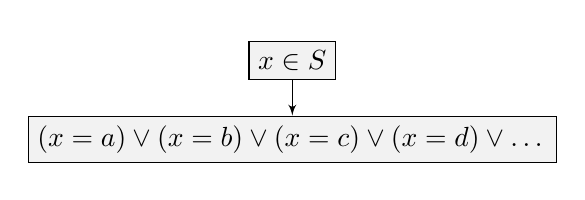
\begin{tikzpicture}
\node at (0,.3) {};
\node [block] (upper) at (0,0) {$x \in S$};
\node [block] (lower) at (0,-1) {$(x=a) \vee (x=b) \vee (x=c) \vee (x=d)\vee \dots$};
\path [line] (upper) -- (lower);
\node at (0,-1.3) {};
\end{tikzpicture}
\end{center}
\end{bmethod}
\begin{example}
Let $S = \{2, 4, 6, 7, 13\}$. Suppose we were given the information that $x \in S$. Then we can conclude that $x=2$ or $x=4$ or $x=6$ or $x=7$ or $x=13$. 
\end{example}
\begin{example}
Let $T = \{2, 4, 6, 8, 10, 12, \dots\}$. If we were told that $y \in T$, then we can conclude that $y = 2$ or $y=4$ or $y=6$ or so on. In other words, we could conclude that $y$ is a positive even integer.
\end{example}

\begin{bmethod}{Proving $x \in S$ if $S$ is in comma-separated format}{proving-element-in-set-roster}
Suppose $S = \{a,b,c,d,\dots\}$. To prove $x \in S$,
\begin{center}
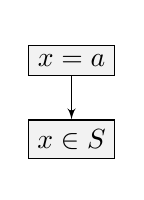
\begin{tikzpicture}
\node at (0,.3) {};
\node [block] (upper) at (0,0) {$x=a$};
\node [block] (lower) at (0,-1) {$x \in S$};
\path [line] (upper) -- (lower);
\node at (0,-1.3) {};
\end{tikzpicture}
\hskip0.1in
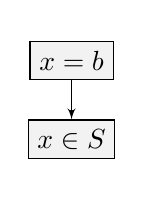
\begin{tikzpicture}
\node at (0,.3) {};
\node [block] (upper) at (0,0) {$x=b$};
\node [block] (lower) at (0,-1) {$x \in S$};
\path [line] (upper) -- (lower);
\node at (0,-1.3) {};
\end{tikzpicture}
\hskip0.1in
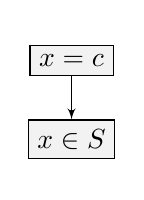
\begin{tikzpicture}
\node at (0,.3) {};
\node [block] (upper) at (0,0) {$x=c$};
\node [block] (lower) at (0,-1) {$x \in S$};
\path [line] (upper) -- (lower);
\node at (0,-1.3) {};
\end{tikzpicture}
\hskip0.1in
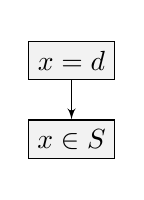
\begin{tikzpicture}
\node at (0,.3) {};
\node [block] (upper) at (0,0) {$x=d$};
\node [block] (lower) at (0,-1) {$x \in S$};
\path [line] (upper) -- (lower);
\node at (0,-1.3) {};
\end{tikzpicture}
\hskip0.1in
\begin{tikzpicture}
\node at (0,.3) {};
\node at (0,-.5) {$\cdots$};
\node at (0,-1.3) {};
\end{tikzpicture}
\end{center}
\end{bmethod}
\begin{example}
Let $S = \{2, 4, 6, 7, 13\}$. Suppose we were given the information that $a = 4$. Then we can conclude that $a \in S$. 
If we were given the information that $b = 7$, we can conclude $b \in S$.
\end{example}
\begin{example}
Let $T = \{2, 4, 6, 8, 10, 12, \dots\}$. If we were told that $y = 38$, then we can conclude that $y \in T$.
\end{example}

\subsection{Set builder with criterion format}

Due to how we must read a set written in set builder with criterion such as $\{x \in \mathbb{Z} : \exists y \in \mathbb{Z} \text{ such that } x = y^2\}$, we obtain methods for using an element belongs to such a set and proving an element belongs to such a set.

\begin{bmethod}{Using $x \in S$ if $S$ is in set builder with criterion format}{using-element-in-set-criterion}
Suppose $S = \{z \in T : P(z)\}$, where $P(z)$ is a predicate. To use $x \in S$,
\begin{center}
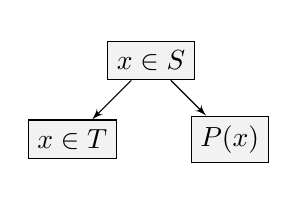
\begin{tikzpicture}
\node at (0,.3) {};
\node [block] (upper) at (0,0) {$x \in S$};
\node [block] (lowerL) at (-1,-1) {$x \in T$};
\node [block] (lowerR) at (1,-1) {$P(x)$};
\path [line] (upper) -- (lowerL);
\path [line] (upper) -- (lowerR);
\node at (0,-1.3) {};
\end{tikzpicture}
\end{center}
\end{bmethod}

\begin{example}
Let $S = \{y \in B : P(y)\}$. Say we were told that \fbox{$x \in S$} is true. Then we can conclude that \fbox{$x \in B$} and \fbox{$P(x)$} are true. If we were given information that \fbox{$y \in S$} is true, then we conclude \fbox{$y \in B$} and \fbox{$P(y)$}.
\end{example}
\begin{example}
Let $U = \{m \in C : P(m)\}$. Say we were told that \fbox{$a \in U$} is true. Then we can conclude that \fbox{$a \in C$} and \fbox{$P(a)$} are true.
\end{example}
\begin{example}
Let $Y = \{m \in C : m \text{ bakes cookies}\}$. Say we were told that \fbox{$t \in Y$} is true. Then we can conclude that \fbox{$t \in C$} and \fbox{$t$ bakes cookies} are true.
\end{example}
\begin{example}
Let $L = \{u \in B : u \text{ is a doctor}\}$. Say we were told that \fbox{$e \in L$} is true. Then we can conclude that \fbox{$e \in B$} and \fbox{$e$ is a doctor} are true. On the other hand, if we knew that $f$ is a doctor we could not conclude from this that $f \in B$. Similarly, if we knew $h \in B$, we could not conclude from this that $h$ is a doctor.
\end{example}


\begin{example}
Let $S = \{z \in \mathbb{R} : z-3 \geq 0 \text{ and } z^2 < 19\}$. Say we were told that \fbox{$x \in S$} is true. Then we can conclude that \fbox{$x \in \mathbb{R}$} and \fbox{$x-3 \geq 0$ and $x^2 < 19$} are true. If we were given information that \fbox{$y \in S$} is true, then we conclude \fbox{$y \in \mathbb{R}$} and \fbox{$y-3 \geq 0$ and $y^2 < 19$}.
\end{example}
\begin{example}
Let $B = \{c \in \mathbb{Z} : c > 100 \text{ or } 20 \text{ divides } c\}$. Upon given the information that \fbox{$a \in B$} is true, we conclude \fbox{$a \in \mathbb{Z}$} is true. We also conclude \fbox{$a > 100$ or $20$ divides $a$} is true.
\end{example}
\begin{example}
Let $D = \{r \in \mathbb{R} \mid \sin(r) \geq 0\}$. If we learn \fbox{$s \in D$} is true, we can conclude \fbox{$s \in \mathbb{R}$} and \fbox{$\sin(s) \geq 0$} are true.
\end{example}

\begin{bmethod}{Proving $x \in S$ if $S$ is in set builder with criterion format}{proving-element-in-set-criterion}
Suppose $S = \{z \in T : P(z)\}$, where $P(z)$ is a predicate. To prove $x \in S$,
\begin{center}
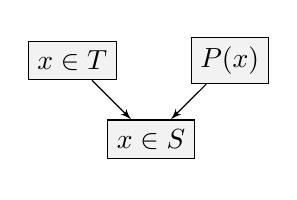
\begin{tikzpicture}
\node at (0,.3) {};
\node [block] (upperL) at (-1,0) {$x \in T$};
\node [block] (upperR) at (1,0) {$P(x)$};
\node [block] (lower) at (0,-1) {$x \in S$};
\path [line] (upperL) -- (lower);
\path [line] (upperR) -- (lower);
\node at (0,-1.3) {};
\end{tikzpicture}
\end{center}
\end{bmethod}


\begin{example}
Let $S = \{y \in B : P(y)\}$. Say we were told \fbox{$x \in B$} and \fbox{$P(x)$} are true. Then we could conclude \fbox{$x \in S$} is true. If we were given information that \fbox{$y \in B$} and \fbox{$P(y)$} are true, we could conclude \fbox{$y \in S$} is true.
\end{example}

\begin{example}
Let $U = \{m \in C : P(m)\}$. Say we were told that \fbox{$a \in C$} and \fbox{$P(a)$} are true. Then we can conclude that \fbox{$a \in U$} is true. 
\end{example}
\begin{example}
Let $Y = \{m \in C : m \text{ bakes cookies}\}$. Say we were told that \fbox{$t \in C$} and \fbox{$t$ bakes cookies} are true. Then we can conclude that  \fbox{$t \in Y$} is true. 
\end{example}
\begin{example}
Let $L = \{u \in B : u \text{ is a doctor}\}$. Say we were told that \fbox{$e \in B$} and \fbox{$e$ is a doctor} are true. Then we can conclude that \fbox{$e \in L$} is true. On the other hand, if we knew that $f$ is a doctor we could not conclude from this that $f \in B$. Similarly, if we knew $h \in B$, we could not conclude from this that $h$ is a doctor.
\end{example}



\begin{example}
Let $S = \{z \in \mathbb{R} : z-3 \geq 0 \text{ and } z^2 < 19\}$. Suppose we know \fbox{$x \in \mathbb{R}$} is true and also know \fbox{$x-3 \geq 0$ and $x^2 < 19$} is true. Then we could conclude \fbox{$x \in S$} is true. If we proved \fbox{$y \in \mathbb{R}$} and also proved that \fbox{$y-3 \geq 0$ and $y^2 < 19$} is true, then we could use these two new facts to conclude that \fbox{$y \in S$} is true.
\end{example}
\begin{example}
Let $B = \{c \in \mathbb{Z} : c > 100 \text{ or } 20 \text{ divides } c\}$. Upon given the information \fbox{$a \in \mathbb{Z}$} along with the information that \fbox{$a > 100$ or $20$ divides $a$}, we could conclude that \fbox{$a \in B$} is true.
\end{example}
\begin{example}
Let $D = \{r \in \mathbb{R} \mid \sin(r) \geq 0\}$. If we learn or prove that \fbox{$m \in \mathbb{R}$} and also prove that \fbox{$\sin(m) \geq 0$}, then we can use this information to conclude that \fbox{$m \in D$} is true.
\end{example}

\subsection{Build running through set format}

Instead of being burdened with another ``using $x \in S$'' flowchart and another ``proving $x \in S$'' flowchart, you may prefer ignoring the new flowcharts introduced here and instead converting the ``gather using running set'' set notation $S = \{f(c) : c \in R \}$ into the ``set-builder with criterion'' set notation $S = \{z : \exists c \in R \text{ s.t. } z=f(c)\}$.

\begin{bmethod}{Using $x \in S$ if $S$ is in build running through set format}{using-element-in-set-running}
If $S = \{f(c) : c \in R \}$, first rewrite $S$ as $S = \{z : \exists c \in R \text{ s.t. } z=f(c)\}$. To use $x \in S$,
\begin{center}
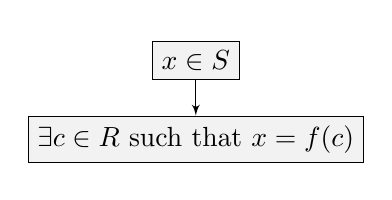
\begin{tikzpicture}
\node at (0,.3) {};
\node [block] (upper) at (0,0) {$x \in S$};
\node [block] (lower) at (0,-1) {$\exists c \in R$ such that $x = f(c)$};
\path [line] (upper) -- (lower);
\node at (0,-1.3) {};
\end{tikzpicture}
\end{center}
\end{bmethod}
\begin{example}
Let $J = \{ 5c + 2 : c \in \mathbb{Z}\}$. We may directly use the method just mentioned, but it is nice to rewrite the set $J$ by writing $J = \{ v : \text{there exists } c \in \mathbb{Z} \text{ such that } v=5c+2\}$. Then if we knew (or were told) that $r \in J$, then we could conclude that there exists $c \in \mathbb{Z}$ such that $m=5c+2$.
\end{example}

\begin{example}
From Example~\ref{example:KmsquaredmR} recall we defined $K = \{ m^2 : m \in \mathbb{R}\}$
which we could rewrite $K = \{ b : \exists m \in \mathbb{R} \text{ such that } b = m^2\}$.
If we knew that \fbox{$y \in K$} we could conclude \fbox{there exists $m \in \mathbb{R}$ such that $y=m^2$} is true.
\end{example}
\begin{example}
Recall the set $L = \{ \sqrt{p} : p \in \mathbb{Z}\}$ from Example~\label{example:Lsqrtp-with-pinZ}
could be rewritten $L = \{u : \exists p \in \mathbb{Z} \text{ such that } u = \sqrt{p}\}$.
If we knew that \fbox{$c \in L$} we could conclude \fbox{there exists $p \in \mathbb{Z}$ such that $c=\sqrt{p}$}.
\end{example}
\begin{example}
Recall the set $M = \{ \cos(n\pi) \mid n \in \mathbb{Z}\}$ from Example~\label{example:Mcosnpi}
could be rewritten $M = \{ a : \exists n \in \mathbb{Z} \text{ such that } a = \cos(n\pi)\}$.
Say we knew \fbox{$h \in M$} is true. Then we could conclude\\ \fbox{there exists $n \in \mathbb{Z}$ such that $h=\cos(n\pi)$} is true.
\end{example}


\begin{bmethod}{Proving $x \in S$ if $S$ is in build running through set format}{proving-element-in-set-running}
If $S = \{f(c) : c \in R \}$, first rewrite $S$ as $S = \{z : \exists c \in R \text{ s.t. } z=f(c)\}$. To prove $x \in S$,
\begin{center}
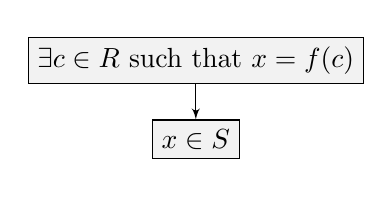
\begin{tikzpicture}
\node at (0,.3) {};
\node [block] (upper) at (0,0) {$\exists c \in R$ such that $x = f(c)$};
\node [block] (lower) at (0,-1) {$x \in S$};
\path [line] (upper) -- (lower);
\node at (0,-1.3) {};
\end{tikzpicture}
\end{center}
\end{bmethod}
\begin{example}
Let $J = \{ 5c + 2 : c \in \mathbb{Z}\}$. We may directly use the method just mentioned, but it is nice to rewrite the set $J$ by writing $J = \{ v : \text{there exists } c \in \mathbb{Z} \text{ such that } v=5c+2\}$. Then if we knew (or were told) that \fbox{there exists $c \in \mathbb{Z}$ such that $m=5c+2$}, we could then conclude that \fbox{$m \in J$}.
\end{example}

\begin{example}
From Example~\ref{example:KmsquaredmR} recall we defined $K = \{ m^2 : m \in \mathbb{R}\}$
which we could rewrite $K = \{ b : \exists m \in \mathbb{R} \text{ such that } b = m^2\}$.
If we knew that \fbox{there exists $m \in \mathbb{R}$ such that $y=m^2$} we could conclude \fbox{$y \in K$}.
\end{example}
\begin{example}
Recall the set $L = \{ \sqrt{p} : p \in \mathbb{Z}\}$ from Example~\label{example:Lsqrtp-with-pinZ}
could be rewritten $L = \{u : \exists p \in \mathbb{Z} \text{ such that } u = \sqrt{p}\}$.
If we knew that \fbox{there exists $p \in \mathbb{Z}$ such that $c=\sqrt{p}$} we could conclude \fbox{$c \in L$}.
\end{example}
\begin{example}
Recall the set $M = \{ \cos(n\pi) \mid n \in \mathbb{Z}\}$ from Example~\label{example:Mcosnpi}
could be rewritten $M = \{ a : \exists n \in \mathbb{Z} \text{ such that } a = \cos(n\pi)\}$.
If we knew that \fbox{there exists $n \in \mathbb{Z}$ such that $h=\cos(n\pi)$} we could conclude \fbox{$h \in M$}.
\end{example}



\begin{example}\label{example:range-preview}
Let $R = \{ \sin(x) : x \in \mathbb{Q}\}$. We may directly use the method just mentioned, but it is nice to write $R = \{ c : \text{there exists } x \in \mathbb{Q} \text{ such that } c=\sin(x)\}$. Then if we knew (or were told) that there exists $x \in \mathbb{Q}$ such that $c=\sin(x)$, we could then conclude that $c \in R$.
\end{example}

\subsection{Summary}

Later sections of the book will refer to these two methods (which in turn refer back to previous methods in this chapter).

\begin{bmethod}{Using the fact that an object is an element of a set}{using-set-membership}
Determine which format of set notation is being used. (Method~\ref{method:tell-apart-set-notations} may help.)
If the set is written in comma-separated format, refer to Method~\ref{method:using-element-in-set-roster}.
If the set is written in set builder with criterion format, refer to Method~\ref{method:using-element-in-set-criterion}.
If the set is written in build running through set format, rewrite the set in set builder with criterion format using Method~\ref{method:convert-running-set}, or for a direct method, refer to Method~\ref{method:using-element-in-set-running}.
\end{bmethod}

\begin{bmethod}{Proving that an object is an element of a set}{proving-set-membership}
Determine which format of set notation is being used. (Method~\ref{method:tell-apart-set-notations} may help.)
If the set is written in comma-separated format, refer to Method~\ref{method:proving-element-in-set-roster}.
If the set is written in set builder with criterion format, refer to Method~\ref{method:proving-element-in-set-criterion}.
If the set is written in build running through set format, rewrite the set in set builder with criterion format using Method~\ref{method:convert-running-set}, or for a direct method, refer to Method~\ref{method:proving-element-in-set-running}.
\end{bmethod}
\begin{example}
Let $Z =\{x \in G \mid \forall g \in G, gx=xg\}$. Notice that this set is in set builder with criterion format.

Suppose you needed to prove that $g \in Z$. Unfortunately, the definition of $Z$ already has a $g$ written, but this is just a notation clash. Think back to the confusion of a struggling algebra student in trying to evaluate $f(x^2+3x)$ if $f$ was defined by $f(x)=\sin(\sqrt{x}+3)$. In this situation, we would encourage the confused student to write $f(y)=\sin(\sqrt{y}+3)$.

In the same way, noting that the universally-quantified $g$ in the definition of $Z$ is a placeholder variable, let us rewrite $Z$ by writing $Z =\{x \in G \mid \forall y \in G, yx=xy\}$. Then, it becomes clearer to us what we have to do to prove that $g \in Z$.

Noting that $g$ would take the place of $x$, we need to a post-substituted version of the statements before and after the vertical bar. Namely, if we prove that $g \in G$ and also prove that for all $y \in G$, we have $yg=gy$, then we can conclude that $g \in G$.
\end{example}

\subsection{Assorted examples and exercises for set membership rules}

Given $S = \{z \in T : P(z)\}$, Method~\ref{method:using-element-in-set-criterion} says knowing $x \in S$ leads to knowing both $x \in T$ and $P(x)$, while Method~\ref{method:proving-element-in-set-criterion} says knowing both $x \in T$ and $P(x)$ lets us conclude $x \in S$. These are the only rules of inference. People who are new to proof may be tempted to make the following errors:
\begin{bwarning}{}{builder-part1-implies-part2}
Suppose the set $S$ is defined by $S = \{z \in T : P(z)\}$. Then knowing \fbox{$z \in T$} is true does not allow you to conclude that \fbox{$P(z)$} is true. Similarly, knowing \fbox{$y \in T$} does not mean that we know anything about whether \fbox{$P(y)$} is true.
\end{bwarning}
\begin{bwarning}{}{builder-part2-implies-part1}
Suppose the set $S$ is defined by $S = \{z \in T : P(z)\}$. Then knowing \fbox{$P(z)$} is true does not allow you to conclude that \fbox{$z \in T$} is true.  Similarly, knowing \fbox{$P(y)$} does not mean that we know anything about whether \fbox{$y \in T$} is true.
\end{bwarning}

\begin{bwarning}{}{convert-set-notation-from-wrong-setup}
Method~\ref{method:convert-running-set} is a procedure that starts with a set in build running through set format and rewrites the set in set builder with criterion format. Do not apply the method to a set that is already in set builder with criterion format.
\end{bwarning}

\begin{example}
Consider the set $S = \{x \in \mathbb{Z} : x = x^2\}$. Note that the only integers which satisfy the property that they are equal to their square happen to be $x=1$ or $x=0$. More importantly, note that $x \in \mathbb{Z}$ does not imply that $x=x^2$.
\end{example}

\begin{example}
Let's say that someone defined the set $S$ for us by writing $S = \{z \in L : z \text{ has cool sneakers}\}$. Note that $S$ is written in set builder with criterion format.
\begin{itemize}
\item Say we knew \fbox{$x \in S$} is true. Following Method~\ref{method:using-element-in-set-criterion}, we can conclude \fbox{$x \in L$} and \fbox{$x$ has cool sneakers} are both true.
\item Say we knew \fbox{$c \in S$} is true. Following Method~\ref{method:using-element-in-set-criterion}, we can conclude \fbox{$c \in L$} and \fbox{$c$ has cool sneakers} are both true.
\item Say we knew \fbox{$x \in L$} and \fbox{$x$ has cool sneakers} are both true. Following Method~\ref{method:proving-element-in-set-criterion}, we can conclude that \fbox{$x \in S$} is true. 
\item Say we knew \fbox{$h \in L$} and \fbox{$h$ has cool sneakers} are both true. Following Method~\ref{method:proving-element-in-set-criterion}, we can conclude that \fbox{$h \in S$} is true. 
\item If we know \fbox{$m \in L$} is true, it is an error to conclude \fbox{$m$ has cool sneakers} which is addressed in Warning~\ref{warning:builder-part1-implies-part2}.
\item If we know \fbox{$j$ has cool sneakers} is true, it is an error to conclude \fbox{$j \in L$} which is addressed in Warning~\ref{warning:builder-part2-implies-part1}.
\end{itemize}
\end{example}

\begin{example}
Let $B=\{x \in A : \text{Sam writes a check to } x\}$, a set written in  set builder with criterion format.
\begin{itemize}
\item Say we knew \fbox{$m \in B$} is true. By Method~\ref{method:using-element-in-set-criterion}, we conclude \fbox{$m \in A$} and \fbox{Sam writes a check to $m$} are true.
\item Say we knew \fbox{$g \in A$} and \fbox{Sam writes a check to $g$} are true. Following Method~\ref{method:proving-element-in-set-criterion}, we conclude \fbox{$g \in B$} is true. 
\item If we know \fbox{$r \in A$} is true, it is an error to conclude \fbox{Sam writes a check to $r$} which is addressed in Warning~\ref{warning:builder-part1-implies-part2}.
\item If we know \fbox{Sam writes a check to $k$} is true, it is an error to conclude \fbox{$k \in A$} which is addressed in Warning~\ref{warning:builder-part2-implies-part1}.
\end{itemize}
\end{example}

\begin{bwarning}{}{meaningless-set-rewrite}
Say you are given the set $S = \{z \in L : z \text{ has cool sneakers}\}$. Say that you know $u \in S$. Then it is not truly advancing your proof forward to write
\[S = \{u \in L : u \text{ has cool sneakers}\}.\]
This is simply rewriting the definition of $S$ using a new placeholder variable, and runs close to the danger of accidentally ``redefining'' $S$ (note: nothing should ever be redefined). Instead of doing this kind of symbol manipulation that does not advance your proof forward, you should look at
\[S = \{z \in L : z \text{ has cool sneakers}\}\]
and based on $u \in S$, you should conclude two things:
\begin{itemize}
\item $u \in L$.
\item $u$ has cool sneakers.
\end{itemize}
\end{bwarning}

% Mathematical examples (some in builder, some in running) which are not as haywire as the ones found in the next subsection: slowly introduce running through two sets, slowly introduce converting set notations
\begin{example}
You are given the set $U = \{y \in \mathbb{Z} : y^2 < 15\}$. If you are told that $x \in U$, then you can conclude $x \in \mathbb{Z}$ and can also conclude $x^2 < 15$. Warning~\ref{warning:meaningless-set-rewrite} tells us it's pointless (and borderline dangerous) to write $U = \{x \in \mathbb{Z} : x^2 < 15\}$. If we know that $a \in \mathbb{Z}$, we cannot conclude $a^2 < 15$. If we know $b^2 < 15$, we cannot conclude $b \in \mathbb{Z}$. If we know $c \in \mathbb{Z}$ and we know $c^2 <15$, then we can conclude $c \in U$.
\end{example}
\begin{example}
You are given the set $U = \{y^2 + 15 : y \in \mathbb{Z}\}$. This is in build running through set format, so we rewrite the set as $U = \{h : \exists y \in \mathbb{Z} \text{ such that } h = y^2+15\}$. If we are told that $s \in U$, it is pointless (and dangerous) to write $U = \{s : \exists y \in \mathbb{Z} \text{ such that } s = y^2+15\}$. Instead, we simply conclude that there exists $y \in \mathbb{Z}$ such that $s = y^2+15$. If we know that there exists $t \in \mathbb{Z}$ such that $c = t^2+15$, this is the same as knowing that there exists $y \in \mathbb{Z}$ such that $c = y^2+15$, so we can conclude that $c \in U$.
\end{example}
\begin{example}
Say that $L = \{a^2+b^2 : a \in \mathbb{Z}, b \in \mathbb{Z}\}$. Then $L$ is built running through two sets. If we know that $h \in L$, we can conclude that there exists $a \in \mathbb{Z}$ and there exists $b \in \mathbb{Z}$ such that $h = a^2+b^2$.
\end{example}

\begin{exercise}
If the set $Q$ is defined to be $Q=\{x \in X : d(x,a)<r\}$ what can you conclude if you know \fbox{$w \in Q$}?
\end{exercise}
\begin{proof}[Solution to exercise]
Since $w \in Q$, we can conclude $w \in X$ and we can also conclude $d(w,a)<r$.
\end{proof}

\begin{exercise}
If the set $Q$ is defined to be $Q=\{x \in X : d(x,a)<r\}$ what do you have to do to prove \fbox{$c \in Q$}?
\end{exercise}
\begin{proof}[Solution to exercise]
To prove $c \in Q$, we must prove $c \in X$ and we must also prove $d(c,a)<r$.
\end{proof}

\begin{exercise}
If the set $E$ is defined to be $E=\{g \cdot x \mid g \in G\}$ what can you conclude if you know \fbox{$j \in E$}?
\end{exercise}
\begin{proof}[Solution to exercise]
First, we rewrite the set $E$ in set builder with criterion format. So,
\[E = \{s \mid \exists g \in G \text{ such that } s=g \cdot x\}.\]
Note that $s$ is placeholder variable, and all of the $s$'s above could have been $t$'s (but not $g$'s or $x$'s).

Since $j \in E$, we get to conclude $\exists g \in G$ such that $j = g \cdot x$.
\end{proof}

\begin{exercise}
If the set $E$ is defined to be $E=\{g \cdot x \mid g \in G\}$ what do you have to do to prove \fbox{$k \in E$}?
\end{exercise}
\begin{proof}[Solution to exercise]
First, we rewrite the set $E$ as
\[E = \{t \mid \exists g \in G \text{ such that } t=g \cdot x\}.\]
Note that $t$ is just a placeholder variable, and all of the $t$'s above could have been $u$'s (but not $g$'s or $x$'s).

To prove $k \in E$, we have to first prove $\exists g \in G$ such that $k = g \cdot x$.
\end{proof}



\subsection*{Exercises from actual mathematical literature}

Consider the following sets:
\begin{itemize}
\item $A = \{a \in G \mid ax = xa \text{ for all } x \in G\}= \{a \in G \mid \text{for all } x \in G,\,\, ax = xa \}$ from pg. 66 of Joseph Gallian. \emph{Abstract Algebra}. (8th ed.)
\item $B = \{z \in (\mathbb{C}^*)^n : f(z)=0 \text{ for all } f \in I\}$ from pg. 17 of Diana Maclagan, Bernd Sturmfels. \emph{Introduction to Tropical Geometry}.
\item $C = \{f(x) : x \in [x_{i-1}, x_i]\}$ from pg. 276 of Matthew A. Pons. \emph{Real Analysis for the Undergraduate}.
\item $D = \{x \mid x \in A \text{ or } x \in B\}$ from pg. 5 of James R. Munkres. \emph{Topology}.
\item $E = \{g \cdot x : g \in G\}$ from pg. 116 of Joseph Rotman. \emph{Galois Theory}.
\item $F = \{T(v) : v \in V\}$ from pg. 43 of Sheldon Axler. \emph{Linear Algebra Done Right}. (2nd ed.)
\item $G = \{4,3,2\}$ from pg. 217 of Branko Gr\"unbaum. \emph{Configurations of Points and Lines}.
\item $H = \{x \in P : cx=c_0\}$ from pg. 130 of G\"unter M. Ziegler. \emph{Lectures on Polytopes}.
\item $I = \{y_F + \lambda(x-y_F) : x \in G, \lambda \geq 0\}$ from pg. 32 of Rekha R. Thomas. \emph{Lectures in Geometric Combinatorics}.
\item $J = \{p, \rho(p), \rho^2(p),\dots, \rho^{n-1}(p)\}$ from pg. 39 of Ronald Solomon. \emph{Abstract Algebra}.
\item $K = \{B \in W^P \mid B \not= A, \mu^{-1}[A] \text{ and } \mu^{-1}[B] \text{ are adjacent}\}$ from pg. 168 of Alexandre V. Borovik, I. M. Gel'fand, and Neil White. \emph{Coxeter Matroids}.
\item $L = \{(0,y) \mid y \in Y\}$ from pg. 61 of Gerald Teschl. \emph{Topics in Real and Functional Analysis}.
\item $M = \{r \in \mathbb{R}^n : x+ \lambda r \in P \text{ for all } x \in P \text{ and } \lambda \in \mathbb{R}_{\geq 0}\}$ from pg. 97 of Michele Conforti, G\'erard Cornu\'ejols, Giacomo Zambelli. \emph{Integer Programming}.
\item $N = \{\mu_1b_1+\mu_2b_2 : (\mu_1,\mu_2) \in \mathbb{Z}^2_+\}$ from pg. 110 of Jes\'us A. De Loera, Raymond Hemmecke, Matthias K\"oppe. \emph{Algebraic and Geometric Ideas in the Theory of Discrete Optimization}.
\item $O = \{(a_1,\dots,a_n) \in k^n \mid f(a_1,\dots,a_n)=0 \text{ for all } f \in S\}$ from pg. 2 of William W. Adams, Philippe Loustaunau. \emph{An Introduction to Gr\"obner Bases}.
\item $P = \{f \in V^* : |f(x)|\leq 1 \text{ for all } x \in U\}$ from pg. 116 of Alexander Barvinok. \emph{A Course in Convexity}.
\item $Q = \{x \in X : d(x,a) < r\}$ from pg. 16 of Joseph Muscat. \emph{Functional Analysis}.
\item $R = \{x \mid 0 \leq T(x) \leq s\}$ from pg. 77 of Manfred Einsiedler, Thomas Ward. \emph{Ergodic Theory with a view towards Number Theory}.
\item $S = \{r \in \mathbb{Q} : \text{for some } a \in A \text{ and } c \in C,\,\, r= a+c\}$ from pg. 14 of Charles Chapman Pugh. \emph{Real Mathematical Analysis}.
\item $T = \{x : \bar{A}x=0\}$ from \'Eva Tardos, A Strongly Polynomial Algorithm to Solve Combinatorial Linear Programs, \emph{Operations Research} 34(2):250--256.
\item $U = \{i_0 + i_1 \omega + i_2 \omega^2+i_3\omega^3 : i_o,i_1,i_2,i_3 \in \mathbb{Z}, |i_j|\leq m\}$ from pg. 51 of Ji\v{r}i Matou\v{s}ek. \emph{Lectures on Discrete Geometry}.
\end{itemize}
For each set defined above,
\begin{itemize}
\item Determine if the notation is comma-separated format, set builder notation with criterion, or set builder format with a running set used to ``gather'' elements.
\item In the case of the \underline{running set}, rewrite as \underline{set builder notation with criterion}.
\item Write out a flowchart of \emph{using} $x$ in the set. Write a flowchart for \emph{proving} $x$ in the set. (Because of the converting of ``running set'' notation, you should \emph{never} use the last row of the reference.) What about using $g$ in the set? Proving $g$ in the set? (Try \emph{any} letter -- not just $x$ or $g$.)
\end{itemize}

\section{Properties of sets}

\begin{bdefinition}{Subset}{subset}
A set $S$ is a \defn{subset}\index{subset} of the set $T$ if every element of $S$ is an element of $T$. In other words, $S$ is a \defn{subset} of $T$ if the implication ``if $x \in S$, then $x \in T$'' is true. We write $S \subseteq T$ to denote $S$ is a subset of $T$.
\end{bdefinition}
\begin{example}
Let $S = \{3,4\}$ and $T = \{3,4,5,6\}$. Then $S$ is a subset of $T$ since every element of $S$ is an element of $T$. Note that $T$ is not a subset of $S$.
\end{example}
\begin{example}
Let $C = \{3,4,5\}$ and $D = \{3,4,5\}$. Then $C \subseteq D$ since every element of $C$ is an element of $D$. Also, $D \subseteq C$.
\end{example}
\begin{example}\label{example:number-set-subsets}
Recall $\mathbb{Z}$, $\mathbb{Q}$, $\mathbb{R}$, and $\mathbb{C}$ are the sets of integers, rationals, reals, and complexes, respectively. Then
$\mathbb{Z} \subseteq \mathbb{Q}$ and
$\mathbb{Q} \subseteq \mathbb{R}$ and
$\mathbb{R} \subseteq \mathbb{C}$.
\end{example}

\begin{exercise}
In Exercise~\ref{exercise:disjunction-checklist}, you were asked to consider what are things that must be addressed in writing a definition of disjunction. Similarly, what are things that you must address when writing a definition for subset? What things \emph{don't} matter?
\end{exercise}


\begin{bmethod}{How to prove a set $A$ is subset of the set $B$}{proving-subset}
Let $A$ and $B$ be sets. Informed by Definition~\ref{definition:subset}, to prove that $A$ is a subset of $B$, we should show that every element of the set $A$ is an element of the set $B$. To do this, write \fbox{Let $x \in A$ be arbitrary.} Then prove that $x \in B$. Said differently, since $A \subseteq B$ is logically equivalent to \fbox{$s \in A$ implies $s \in B$} you should assume $s \in A$ and then prove $s \in B$.
\vskip6pt
Once you say ``Let $x \in A$ be arbitrary'' you will need to use the fact that $x$ is an element of $A$, following Method~\ref{method:using-set-membership}. You will likely need to use the facts obtained through that method to prove that $x \in B$, following Method~\ref{method:proving-set-membership}.
\vskip6pt
If $x$ has already been used in your proof, it is good practice to select a different variable. Perhaps you can let $\vartheta \in A$, and then prove that $\vartheta \in B$.
\end{bmethod}
As an example, let us prove the following:
\begin{theorem}\label{theorem:subset-10-5}
Let $A$ be the set of all multiples of $10$. Let $B$ be the set of all multiples of $5$. Then $A \subseteq B$.
\end{theorem}
\begin{proof}
Let $A$ be the set of all multiples of $10$. Let $B$ be the set of all multiples of $5$. Let $c \in A$. Then $c$ is a multiple of $10$. In other words, $10$ divides $c$. Thus, there exists an integer $k$ such that $10k=c$. Rewriting the left side, we have $5 \cdot 2 \cdot k=c$. Let $r=2k$. Then $5r=5(2k)=(5\cdot2)k=10k=c$. Since $5r=c$ and $r$ is an integer, $5$ divides $c$, which proves that $c$ is a multiple of $5$. Therefore $c \in B$.

We proved that $c \in A$ implies that $c \in B$, so $A$ is a subset of $B$.
\end{proof}

Other facts follow from the subset inclusions mentioned in Example~\ref{example:number-set-subsets}, such as $\mathbb{Z} \subseteq \mathbb{R}$. In fact, you should prove:
\begin{theorem}
Let $A$, $B$ and $C$ be sets. If $A \subseteq B$ and $B \subseteq C$, then $A \subseteq C$.
\end{theorem}
\begin{exercise}
Prove: for all sets $S$, one has $S \subseteq S$.
\end{exercise}

\begin{bmethod}{How to use a set $A$ is subset of the set $B$}{using-subset}
Let $A$ and $B$ be sets. Informed by Definition~\ref{definition:subset}, to prove that $A$ is a subset of $B$, since $A \subseteq B$ is logically equivalent to $x \in A$ implies $x \in B$, as soon as you know $m \in A$, then you can conclude $m \in B$. If you do not know of a specific element of $A$, then you cannot use $A \subseteq B$.
\end{bmethod}
\begin{bwarning}{}{}
It is an error to take the fact $A \subseteq B$ and then write \fbox{$x \in A$ and $x \in B$}. This is turning a conjunction into an implication.
\end{bwarning}

\begin{bwarning}{Membership versus subset}{membership-versus-subset}
Recall that $x \in B$ means that $x$ is a member of the set $B$, and that $x \subseteq B$ means that $x$ is a subset of the set $B$. While this may look strange, it is only because we generally stick to the convention that sets are named with capital letters, but there are times that this convention must be suspended.

Aside from how these two look, $x \in B$ and $x \subseteq B$ really say different things, and one should not be written for the other. For instance, if $B = \{7,9\}$, then we can write $7 \in B$. We cannot write $7 \subseteq B$, because $7$ is not a set.
\end{bwarning}

\begin{bwarning}{Do not ``assume $A$''}{}
When tasked with proving that the set $A$ is a subset of the set $B$, it is tempting to say that you need to ``assume $A$'' and then ``prove $B$.'' However, this does not make sense. Saying ``assume $A$'' makes it sound like $A$ is either true or false. However, we should recall Warning~\ref{warning:set-not-proposition}: a set is not a proposition, so a set is neither true nor false. The same comment applies to saying ``prove $B$.'' A set cannot be proved: a set is a collection of objects, and is neither true nor false. If $A$ and $B$ are both sets, then the same error of thought occurs in saying ``if $A$ is true, then $B$ is true.''
\end{bwarning}

\begin{bwarning}{}{}
When proving that $A$ is a subset of $B$, the second sentence in Definition~\ref{definition:subset} shows we are proving an implication. Therefore, near the end of the proof, it is incorrect to say ``Since $x$ is in $A$ and $x$ is in $B$, we conclude $A$ is a subset of $B$.''
\vskip6pt
Recall from Warning~\ref{warning:conjunction-not-implication} that $p \wedge q$ does not have the same meaning as $p \rightarrow q$. The correct way to conclude would be to write ``Since we proved that $x \in A$ implies that $x \in B$, we conclude $A$ is a subset of $B$.''
\end{bwarning}
In our concluding sentence in the proof of Theorem~\ref{theorem:subset-10-5}, we said $c \in A$ implies $c \in B$. We did \emph{not} say, for example, $c \in A$ and $c \in B$, since an implication is not the same as a conjunction. Similarly, we didn't say that $A$ is true, because a set is neither true nor false.

\begin{bdefinition}{Set equality\index{set equality}}{set-equality}
Two sets $A$ and $B$ are equal if each set is a subset of the other. In this case, we write $A=B$. In other words, if $A$ and $B$ are sets, we say that $A$ is equal to $B$ and write $A=B$ if $A \subseteq B$ and $B \subseteq A$.
\end{bdefinition}
\begin{bmethod}{How to prove that two sets are equal}{prove-set-equality}
To prove that the set $A$ is equal to the set $B$, informed by Definition~\ref{definition:set-equality}, you must prove that $A$ is a subset of $B$ and that $B$ is a subset of $A$. In light of Method~\ref{method:proving-subset}, you should take an arbitrary element $c \in A$ and prove $c \in B$. Then take an arbitrary element $d \in B$ and then prove $d \in A$.
\end{bmethod}
As an example, let us look at proving the following theorem:
\begin{theorem}
Let $X = \{c \in Y : c \text{ plays tennis}\}$ and let $Y = \{r \in L \mid r \text{ plays volleyball}\}$. If
\begin{itemize}
\item for all $z \in Y$, if $z$ does not play tennis, then $z$ is not an interior designer,
\item for all $p \in L$, if $p$ plays volleyball, then $p$ is an interior designer; and
\end{itemize}
then $X = Y$.
\end{theorem}
We will annotate this proof with many references. (The references should not really be included in the proof, but are there for your convenience.) While the statement to prove is $X=Y$, the set up of the theorem comes with two definitions (the definition of the set $X$ and the definition of the set $Y$) alongside two hypotheses (provided in the bullet list).
\begin{proof}
To prove that $X=Y$, following Method~\ref{method:prove-set-equality} we need to prove $X \subseteq Y$ and also prove $Y \subseteq X$.

First, we will prove that $X \subseteq Y$. To prove this, following Method~\ref{method:proving-subset}, let $m \in X$ be arbitrary.
Following Method~\ref{method:using-set-membership}, we are directed to Method~\ref{method:using-element-in-set-criterion}, based on format/notation of the definition of $X$. Thus, $m \in Y$ and $m$ plays tennis. Specifically, following Method~\ref{method:using-conjunction}, $m \in Y$. Since we have proved that $m \in X$ implies $m \in Y$, this concludes the proof that $X \subseteq Y$.

We now will prove that $Y \subseteq X$.  To prove this, following Method~\ref{method:proving-subset}, let $u \in Y$ be arbitrary.
Following Method~\ref{method:using-set-membership}, we are directed to Method~\ref{method:using-element-in-set-criterion}, since $Y$ is also written in set builder with criterion format. From this, we conclude $u \in L$. We also conclude $u$ plays volleyball. Since $u \in L$, this fact together with the second hypothesis (following Method~\ref{method:using-forall}), we conclude that the implication ``if $u$ plays volleyball, then $u$ is an interior designer'' is true. From this implication and the earlier fact that $u$ plays volleyball, by Method~\ref{method:modus-ponens}, we conclude that $u$ is an interior designer.

Since $u \in Y$, combined with the first hypothesis, following Method~\ref{method:using-forall}, we get the implication ``if $u$ does not play tennis, then $u$ is not an interior designer.'' But earlier, we already learned that $u$ is an interior designer, so combined with the new implication, following Method~\ref{method:modus-tollens}, we get that $u$ plays tennis. Since $u \in Y$ and $u$ plays tennis, following Method~\ref{method:proving-element-in-set-criterion}, we conclude that $u \in X$. We have now proved that $u \in Y$ implies $u \in X$, so our proof that $Y \subseteq X$ is complete.

To conclude, since we have proved $X \subseteq Y$ and also proved $Y \subseteq X$, we conclude that $X=Y$.
\end{proof}

\begin{bdefinition}{}{}
A set $S$ is a \defn{proper subset}\index{proper subset} of the set $T$ if $S$ is a subset of $T$ and $S \not= T$. We write $S \subsetneq T$ to denote that $S$ is a proper subset of $T$.
\end{bdefinition}
\begin{example}
Let $A = \{2,3,4\}$ and $B = \{2,3,4,5,6\}$ and $C=\{2,3,4\}$. Then $A$ is a proper subset of $B$. While $A$ is not a proper subset of $C$, though $A$ is a subset of $C$.
\end{example}
\begin{example}
The set $\mathbb{Z}$ is a proper subset of $\mathbb{Q}$, since $\mathbb{Z} \subseteq \mathbb{Q}$ and $\mathbb{Z} \not= \mathbb{Q}$. One piece of evidence for why $\mathbb{Z} \not= \mathbb{Q}$ is that $\frac23 \in \mathbb{Q}$ but $\frac23 \not\in \mathbb{Z}$.
\end{example}

\begin{example}
Let $D = \{5,6\}$. Then $D$ has four subsets, which are $\{\}$ and $\{5\}$ and $\{6\}$ and $\{5,6\}$. Of these four, the first three are proper subsets of $D$ while the fourth is not a proper subset of $D$.
\end{example}

\begin{bdefinition}{Empty set}{empty-set}
A set consisting of no elements is called an \defn{empty set}\index{empty set}, and is denoted $\emptyset$.
\end{bdefinition}
It may have seemed strange to say ``an empty set'' instead of ``the empty set.'' Let us prove that an empty set is unique, following Method~\ref{method:proving-uniqueness}.
\begin{theorem}
An empty set is unique.
\end{theorem}
\begin{proof}
Let $A$ be an empty set. Let $B$ be an empty set. To prove uniqueness, based on the discussion in Section~\ref{section:uniqueness}, we must prove that $A=B$. To prove $A=B$, following Method~\ref{method:prove-set-equality}, we need to prove $A \subseteq B$ and also prove $B \subseteq A$.

To prove $A \subseteq B$, following Method~\ref{method:proving-subset}, we prove that every element of $A$ is an element of $B$. However since $A$ is an empty set (and has no elements according to Definition~\ref{definition:empty-set}), there is nothing to prove to show that every element of $A$ is an element of $B$. This is already true because there are no elements in $A$. Thus $A \subseteq B$. The argument to prove $B \subseteq A$ is similar.
\end{proof}
Since an empty set is unique, we can now say ``the empty set.'' The empty set is a subset of every set. In other words, for every set $A$, we have $\emptyset \subseteq A$. (You should prove: for every set $A$, it is true that $\emptyset \subseteq A$ is true.)

\begin{bdefinition}{Singleton}{singleton}
A set consisting of exactly one element is called a \defn{singleton}\index{singleton}.
\end{bdefinition}
\begin{example}
The set $\{7\}$ is a singleton. 
\end{example}
\begin{example}
The set $\{7,9\}$ is not a singleton, since this set has more than one element.
\end{example}
It is important to note that $\{7\}$ is different from $7$. For example, if $B = \{7,9\}$, it makes sense to write $\{7\} \subseteq B$. However, writing $7 \subseteq B$ doesn't make any sense, because $7$ is not a set. This is a good chance to revisit Warning~\ref{warning:membership-versus-subset}.

A finite set generalizes the notion of singleton:
\begin{bdefinition}{Finite set, infinite set, cardinality}{cardinality}
Let $A$ be a set. If there exists a non-negative integer $n \in \mathbb{Z}_{\geq 0}$ such that $A$ has exactly $n$ elements, then we say that $A$ is a \defn{finite set}\index{finite set} and the \defn{cardinality}\index{cardinality} of $A$ is $n$, denoted $|A|=n$. If there is no such integer $n$, then $A$ is an \defn{infinite set}.
\end{bdefinition}
\begin{example}
The set $A=\{2,4,6,8,10\}$ is finite and $|A|=5$.
\end{example}
\begin{example}
The set $\{7,8,9\}$ is finite and has cardinality $3$.
\end{example}
\begin{example}
There is no non-negative integer $n$ such that $\mathbb{Q}$ has exactly $n$ elements. So $\mathbb{Q}$ is an infinite set. Similarly, the set $\mathbb{Z}$ is infinite.
\end{example}
\begin{example}
The sets $\mathbb{R}$ and $\mathbb{C}$ are also infinite.
\end{example}

\begin{bdefinition}{Power set}{}
Given a set $B$, the \defn{power set}\index{power set} of $B$ is the set of all subsets of $B$, and is denoted $P(B)$.
\end{bdefinition}
Note that $A \in P(B)$ if and only if $A \subseteq B$.
\begin{example}
Let $B$ be the set $\{7,8\}$. Then $P(B) = \{ \{\}, \{7\}, \{8\},\{7,8\} \}$, which we could also have written  $ \{ \emptyset, \{7\}, \{8\}, B\}$. Every element of $P(B)$ is a subset of $B$. Any set which is a subset of $B$ is an element of $P(B)$. 
\end{example}
\begin{example}\label{example:power-set-789}
Let $B$ be the set $\{7,8,9\}$. Then $P(B) = \{ \{\}, \{7\}, \{8\}, \{9\}, \{7,8\}, \{7,9\}, \{8,9\}, \{7,8,9\}\}$. Each of the eight elements of $P(B)$ is a set.
\end{example}
\begin{remark}
Let $B$ be a set. We have introduced $P(B)$ as the notation for the power set of $B$. Other texts use $\mathbb{P}(B)$, though for those who have studied probability, do not confuse this for the probability of an event $B$, which is usually clear by context.
\end{remark}
\begin{remark}\label{remark:power-set-notation-with-2}
Another common notation is $2^B$. Note that there will never be confusion whether $2^B$ denotes the power set of $B$ or is the process of exponentiation from arithmetic, as long as you first ask yourself, ``Is $B$ a set or a number?''

This notation is used because when $B$ is a finite set, $|P(B)|=2^{|B|}$. In Example~\ref{example:power-set-789}, we had $|B|=3$ and $|P(B)|=2^3$.
\end{remark}

\begin{bremark}{}{}
The objects of a set may be sets themselves! In Example~\ref{example:power-set-789}, we saw the set $\{ \{\}, \{7\}, \{8\}, \{9\}, \{7,8\}, \{7,9\}, \{8,9\}, \{7,8,9\}\}$. In this set, one of the members is the set $\{7,9\}$.
\end{bremark}

\begin{exercise}
Let $X = \{a \in Y : a \text{ teaches geometry}\}$ and let $Y = \{b \in Z \mid b \text{ plays World of Warcraft}\}$. With the assumptions
\begin{itemize}
\item For all $a \in Z$, if $a$ plays World of Warcraft, then $a$ has a Pinterest account.
\item For all $z \in Y$, if $z$ does not teach geometry, then $z$ does not have a Pinterest account.
\end{itemize}
Prove $X = Y$.
\end{exercise}
\begin{proof}
In the first paragraph, we prove $X \subseteq Y$. Let $c \in X$. We will prove that $c \in Y$. Since $c \in X$, we conclude $c \in Y$ and that $c$ teaches geometry. In particular, $c \in Y$. So $X \subseteq Y$.

In the second paragraph, we prove $Y \subseteq X$. So, let $r \in Y$. We will prove $r \in X$. Since $r \in Y$, we obtain the facts $r \in Z$ and $r$ plays World of Warcraft. Since $r \in Z$, the first hypothesis allows us to conclude that if $r$ plays World of Warcraft, then $r$ has a Pinterest account. Since $r$ plays World of Warcraft, this and the previous implication give us $r$ has a Pinterest account, by modus ponens. Since $r \in Y$, the second hypothesis gives us the fact that if $r$ does not teach geometry, then $r$ does not have a Pinterest account. Since $r$ has a Pinterest account, by modus tollens, $r$ teaches geometry. Since $r \in Y$ and $r$ teaches geometry, we conclude $r \in X$.
\end{proof}

\begin{exercise}
Let $C = \{x \in E: x \text{ goes fishing}\}$ and let $B=\{y \in F \mid y \text{ does not like beets}\}$.
Using the hypotheses:
\begin{itemize}
\item $A = P(\emptyset)$, in other words: $A$ is the power set of $\emptyset$.
\item If $E$ is not an element of the power set of $F$, then $A \not= \{\emptyset\}$.
\item $C \subseteq K$
\item For all $k \in K$, if $k$ likes beets, then $k$ does not go fishing.
\end{itemize}
Prove: $C \subseteq B$. % https://www.overleaf.com/project/59ea2670c26a0a765618481f
\end{exercise}
\begin{proof}
To prove that $C \subseteq B$, let $a \in C$. We will prove that $a \in B$. Since $a \in C$, we conclude $a \in E$ and $a$ goes fishing.

Consider the first premise. Now, because $A$ is the power set of $\emptyset$, we know that $A$ is non-empty. More specifically, $A=\{0\}$. By applying modus tollens to the second premise, $E$ is an element in the power set of $F$. In other words, $E \subseteq F$. Since $a \in E$ and $E \subseteq F$, we conclude $a \in F$.

The third premise says $C \subseteq K$ and we already know $a \in C$, so $a \in K$. Since we have an element in $K$, namely $a$, we can apply the fourth premise to learn that if $a$ likes beets, then $a$ does not go fishing. Since $a$ goes fishing, by modus tollens, $a$ does not like beets.

Since $a \in F$ and $a$ does not like beets, $a \in B$. Therefore $C \subseteq B$.
\end{proof}

\begin{exercise}
Let $X = \{c \in G: c \text{ still has MySpace}\}$ and\\let $Z=\{a \in Q \mid \forall b \in B, \text{ if } b \text{ likes to skateboard, then } a \text{ follows } b \text{ on Instagram}\}$. Assuming:
\begin{itemize}
\item $\forall s \in G$, $\exists t \in Z$ such that $s$ follows $t$ on Twitter
\item $X \subseteq B$
\item If $Q$ is not an element of the power set of $F$, then $Z = \emptyset$.
\end{itemize}
Prove: $\forall m \in X$, if $m$ likes to skateboard, then $\exists y \in F$ such that $y$ follows $m$ on Instagram. \quad\href{https://www.sharelatex.com/project/59ea2690c26a0a7656184823}{{\color{red}[key]}}
\end{exercise}
\begin{proof}
Let $m \in X$ be arbitrary. We need to prove if $m$ likes to skateboard, then $\exists y \in F$ such that $y$ follows $m$ on Instagram. Suppose $m$ likes to skateboard. We will prove that there exists a $y \in F$ such that $y$ follows $m$ on Instagram.

Now $m \in X$, so $m \in G$ and $m$ still has MySpace. Since $m \in G$, combining this with the first assumption gives $\exists t \in Z$ such that $m$ follows $t$ on Twitter. Since such a $t$ in $Z$ exists, let $t$ be defined so that $t \in Z$ and $m$ follows $t$ on Twitter.

Because $t \in Z$, we can see that $Z \not= \emptyset$. Then applying modus tollens to the third assumption, we conclude that $Q$ is an element of the power set of $F$. So $Q \subseteq F$.

As another consequence of $t \in Z$, by definition of $Z$, we have $t \in Q$ and also now know that for all $b \in B$, if $b$ likes to skateboard, then $t$ follows $b$ on Instagram.

Since $m \in X$ and the second premise is $X \subseteq B$, we now know $m \in B$. Since we know ``for all $b \in B$, if $b$ likes to skateboard, then $t$ follows $b$ on Instagram'' in particular since $m \in B$, we can conclude that if $m$ likes to skateboard, then $t$ follows $m$ on Instagram.

Since we earlier showed that $t \in Q$ and also showed that $Q \subseteq F$, we have $t \in F$. Since $t \in F$ and $t$ follows $m$ on Instagram, we have proved that there exists a $y \in F$ such that $y$ follows $m$ on Instagram.
\end{proof}

\begin{exercise}
Let $A = \{x \in C : x \text{ writes books and } x \text{ is a barista}\}$, 
let $B = \{y \in D \mid y \text{ sings or } y \text{ has a goldfish}\}$,
and let $C = \{y \in E : y \text{ likes Culvers}\}$. Using the hypotheses
\begin{itemize}
\item For all $z \in E$, if $z$ writes books, then $z$ has a goldfish
\item $C$ is an element of the power set of $E$
\item $\forall j \in D$ if $j$ sings then $j$ runs marathons
\item For all $g \in D$, if $g$ has a goldfish, then $g$ runs marathons.
\item $\forall b \in B$, if $b$ is not a barista, then $b$ does not run marathons
\item $\forall x \in B$, if $x$ runs marathons, then $x$ writes books
\item $\forall z \in C$, if $z$ likes Culvers, then $z$ lives in a pineapple
\item $C \subseteq D$.
\item $B \subseteq C$.
\end{itemize}
prove $A=B$.
\quad\href{https://www.sharelatex.com/project/59ea26b5c26a0a7656184834}{{\color{red}[key]}}
\end{exercise}
\begin{proof}
To prove that the sets $A$ and $B$ are equal, we need to prove $A \subseteq B$ and $B \subseteq A$.

To prove that $A \subseteq B$, let $x \in A$ be arbitrary. We will prove that $x \in B$. Since $x \in A$, we conclude $x \in C$ and $x$ writes books and $x$ is a barista. Just to note this now, to prove that $x \in B$, we will need to prove that $x \in D$ and that $x$ sings or $x$ has a goldfish.  The second premise is that $C \in P(E)$. In other words, $C \subseteq E$. Since $x \in C$ and $C \subseteq E$, we get $x \in E$. The first hypothesis applies to any element in $E$, in particular, to $x \in E$, so we conclude that if $x$ writes books, then $x$ has a goldfish. Since we earlier discovered that $x$ writes books, we use modus ponens to conclude that $x$ has a goldfish.

Now $C \subseteq D$ and since $x \in C$, we conclude $x \in D$. Since we saw that $x$ has a goldfish, it is certainly true that $x$ sings or $x$ has a goldfish, because a disjunction is true when at least one of the propositions is true. Since $x \in D$ and since $x$ sings or $x$ has a goldfish, $x \in B$. This completes the proof of $A \subseteq B$.

To prove that $B \subseteq A$, let $x \in B$ be arbitrary. (Note, we reuse $x$, but have to ignore \emph{everything} from earlier.) We will prove that $x \in A$. In other words, we need to prove that $x \in C$ and that $x$ writes books and $x$ is a barista. Since $x \in B$, by how $B$ is defined, $x \in D$. In addition, $x$ sings or $x$ has a goldfish. (Note, we cannot assume that both $x$ sings and $x$ has a goldfish. We can assume at least one of these two things is true.)

Since at least one of  the propositions ``$x$ sings'' and ``$x$ has a goldfish'' is true, we prove that $x$ runs marathons by cases. Either $x$ sings, or $x$ has a goldfish:
\begin{itemize}
\item Case 1: suppose $x$ sings. Since $x \in D$, the third premise tells us that if $x$ sings, then $x$ runs marathons. By modus ponens, $x$ runs marathons.
\item Case 2: suppose $x$ has a goldfish. Since $x \in D$, the fourth proposition tells us that if $x$ has a goldfish, then $x$ runs marathons. By modus ponens, $x$ runs marathons.
\end{itemize}
In either case (in either situation) $x$ runs marathons. (In other words, no matter what, we know that $x$ runs marathons.) Since $x \in B$, the 6th hypothesis tells us if $x$ runs marathons, then $x$ writes books. So $x$ writes books. Since $x \in B$, the 5th hypothesis tells us if $x$ is not a barista, then $x$ does not run marathons. By modus tollens, $x$ is a barista. So $x$ writes books and $x$ is a barista. Since $x \in B$ and $B \subseteq C$, we conclude $x \in C$. Since $x \in C$ and $x$ writes books and $x$ is a barista, $x \in A$.
\end{proof}

\begin{exercise}
Let $B$ be the set $B = \{x \in D : x\text{ has a puppy}\}$, let $F$ be the set $F = \{z \in E \mid z \text{ commutes by bike}\}$ and $G=\{z \in B : z \text{ commutes by train}\}$.  Using the hypotheses:
\begin{itemize}
\item $C \subseteq E$.
\item for all $c \in C$ and for all $d \in D$, if $c$ supervises $d$, then $c$ commutes by bike and $d$ commutes by train.
\item $A \subseteq C$.
\end{itemize}
Prove: for all $x \in A$, for all $y \in B$, if $x$ supervises $y$, then $x \in F$ and $y \in G$.
\end{exercise}

\begin{exercise}
Use the definitions
\begin{itemize}
\item $X = \{u \in L: u \text{ is a coin collector}\}$
\item $Y = \{m \in M \mid m \text{ likes soda if and only if } m \text{ plays video games}\}$
\end{itemize}
and the hypotheses
\begin{itemize}
\item if $x$ plays video games, then $x$ researches chemistry.
\item $L \subseteq Y$
\item for all $c \in M$, if $c$ researches chemistry, then for all $d \in M$,\,\,$d$ gives $c$ pizza.
\end{itemize}
to prove: for all $y \in Y$, for all $x \in X$, if $x$ likes soda, then $y$ gives $x$ pizza.
\end{exercise}
%\begin{proof}Let $y \in Y$. Let $x \in X$. We will prove if $x$ likes soda, then $y$ gives $x$ pizza. So suppose $x$ likes soda. We will prove $y$ gives $x$ pizza. Since $y \in Y$, we have $y \in M$ and we also have $y$ likes soda if and only if $y$ plays video games. (It turns out that we will never use the biconditional $y$ likes soda if and only if $y$ plays video games.) Since $x \in X$, we have $x \in L$ and $x$ is a coin collector. Since $x \in L$, by the second hypothesis, $x \in Y$. Since $x \in Y$, we have $x \in M$ and we also know the biconditional $x$ likes soda iff $x$ plays video games. \vskip6pt Recall that we supposed $x$ likes soda, so we conclude $x$ plays video games. By the first hypothesis, $x$ researches chemistry. Recall that $x \in M$, so applying the third hypothesis, we know the implication ``if $x$ researches chemistry, then for all $d \in M$,\,\,$d$ gives $x$ pizza'' is true. Recall $x$ researches chemistry. So, for all $d \in M$, we have $d$ gives $x$ pizza. Since $y \in M$, we have $y$ gives $x$ pizza.\end{proof}

\begin{exercise}
Use the definitions
\begin{itemize}
\item $A = \{a \in M: a \text{ likes to study math}\}$
\item $B = \{z \in D: \text{ if } z \text{ has a pet hippo, then } z \text{ does not like to study math}\}$
\item $C = \{c \in D \mid c \text{ writes poetry}\}$
\item $D = \{s \in S : s \text{ likes radishes if and only if } s \text{ writes poetry}\}$
\end{itemize}
and the hypotheses
\begin{itemize}
\item For all $d \in D$, if $d$ does not have a pet hippo, then $d$ likes radishes.
\item $B \subseteq A$
\end{itemize}
to prove: $B \subseteq C$.
\end{exercise}
%\begin{proof}Assume $x \in B$. We will prove $x \in C$. Since $x \in B$, by the second hypothesis, $x \in A$. Since $x \in A$, we conclude $x \in M$ and also conclude $x$ likes to study math. Since $x \in B$, we conclude $x \in D$, and we also learn the implication ``if $x$ has a pet hippo, then $x$ does not like to study math'' is true. But recall $x$ likes to study math, so applying the previous implication (via modus tollens), we get $x$ does not have a pet hippo. Because $x \in D$, by the first hypothesis, we learn the implication ``if $x$ does not have a pet hippo, then $x$ likes radishes'' is true. Since $x$ does not have a pet hippo, we conclude (by modus ponens) that $x$ likes radishes. We learn another fact, also due to the fact that $x \in D$, but this is based on the definition of $D$. Namely, we learn that $x \in S$ and also learn the biconditional ``$x$ likes radishes iff $x$ writes poetry'' is true. Recall that $x$ likes radishes. Thus, $x$ writes poetry. Since $x \in D$ and $x$ likes poetry, $x \in C$. We have proved that $x \in B$ implies $x \in C$, thus we have proved $B \subseteq C$.\end{proof}

\begin{exercise}
Use the definitions
\begin{itemize}
\item $A = \{x \in U : x \text{ works weekends}\}$
\item $C = \{y \in B \mid \text{if } y \text{ works weekends, then } y \text{ manages employees}\}$
\item $D = \{m \in U : m \text{ likes pretzels and } m \text{ pickles veggies}\}$
\item $K = \{k \in S : k \text{ runs a restaurant}\}$
\item $N = \{n \in C : n \text{ likes pretzels if and only if } n \text{ manages employees}\}$
\item $U = \{z \in L \mid z \text{ plays poker}\}$
\end{itemize}
and the hypotheses
\begin{itemize}
\item $D$ is an element of the power set of $K$
\item $U \subseteq N$
\end{itemize}
to prove: for all $x \in A$, if $x$ pickles veggies, then $x$ runs a restaurant.
\end{exercise}
%\begin{proof}Let $x \in A$ be arbitrary. Suppose $x$ pickles veggies. We want to show $x$ runs a restaurant. Since $x \in A$, we have $x \in U$ and $x$ works weekends. Since $x \in U$, we have $x \in L$ and $x$ plays poker. Also, since $x \in U$, by the second hypothesis, $x \in N$. Since $x \in N$, we have $x \in C$ and also have the biconditional ``$x$ likes pretzels iff $x$ manages employees'' is true. Since $x \in C$, we have $x \in B$ and also have the implication ``$x$ works weekends implies $x$ manages employees'' is true. Recalling that we earlier had $x$ works weekends, we conclude $x$ manages employees. This fact together with our earlier biconditional allows us to conclude $x$ likes pretzels. Gathering previous facts, since $x \in U$ and $x$ likes pretzels and $x$ pickles veggies, $x \in D$. By the first hypothesis, $x \in K$. Since $x \in K$, we have $x \in S$ and also learn $x$ runs a restaurant.\end{proof}

\section{Set operations}

Just as Section~\ref{section:logical-operations} introduced logical operations (such as negation, conjunction, disjunction, implication, biconditional) which allowed us to meaningfully combine propositions to get new propositions, set operations (such as union and intersection) allow us to meaningfully combine sets to define new sets:
\begin{bdefinition}{Union}{union}
Let $A$ and $B$ be sets. The \defn{union}\index{union} of $A$ and $B$, denoted $A \cup B$, is the set that satisfies the property that $x \in A \cup B$ if and only if $x \in A$ or $x \in B$. In symbols,
\[ A \cup B = \{ x \mid x \in A \vee x \in B\}.\]
\end{bdefinition}
The definition clearly states that $A \cup B$ is a set.
\begin{example}
Let $A = \{1,2,3,4\}$ and $B=\{3,4,5,6\}$. Then $A \cup B = \{1,2,3,4,5,6\}$. Duplicates may be written optionally, as sets don't keep track of ``how many times'' an element appears. (Sets are only concerned with \emph{if} an element appears.) See Remark~\ref{remark:set-element-repetition}.
\end{example}

\begin{bdefinition}{Intersection}{}
Let $A$ and $B$ be sets. The \defn{intersection}\index{intersection} of $A$ and $B$, denoted $A \cap B$, is the set that satisfies the property that $x \in A \cap B$ if and only if $x \in A$ and $x \in B$. In symbols,
\[ A \cap B = \{ x \mid x \in A \wedge x \in B\}.\]
\end{bdefinition}
The definition states that $A \cap B$ is a set.
\begin{example}
Let $A = \{1,2,3,4\}$ and $B=\{3,4,5,6\}$. Then $A \cap B = \{3,4\}$.
\end{example}
\begin{example}
Let $C = \{7,8,9\}$ and $D=\{9,10,11,12\}$. It is tempting to write $C \cap D =9$, but this is incorrect. We noted that the intersection is a set. Instead, one must write $C \cap D = \{9\}$.
\end{example}

\begin{bdefinition}{Disjoint}{}
Two sets $A$ and $B$ are \defn{disjoint}\index{disjoint} if $A \cap B = \emptyset$.
\end{bdefinition}
Sometimes, this is phrased as $A$ is \defn{disjoint}\index{disjoint} from $B$. Two sets are disjoint if and only if they have no elements in common.
\begin{example}
The sets $\{1,2,3,4\}$ and $\{7,8\}$ are disjoint.
\end{example}
\begin{example}
The sets $\{1,2,3,4\}$ and $\{2,8\}$ are not disjoint.
\end{example}

\begin{bwarning}{}{}
The definition of \underline{disjoint} references the definition of \underline{intersection}, but the two should not be confused with each other. Given sets $C = \{3,8\}$ and $D = \{7,13,18\}$ and $E = \{8,18\}$ it is common for students to say things like $C \cap D$ doesn't exist, but this is not true. The intersection of $C$ and $D$ does exist, and is the empty set. We would say $C$ and $D$ are disjoint because $C \cap D = \emptyset$, but we don't say $C \cap D$ doesn't exist. By analogy, we know that $-5 +5 =0$, but simply because the result of $-5 +5$ is the number $0$, we don't say $-5+5$ doesn't exist.
\vskip6pt
To restate, both $C \cap E$ and $C \cap D$ exist. In the first case, $C \cap E$ is the set $\{8\}$, while in the second case, $C \cap D$ is the set $\{\}$.
\vskip6pt
The intersection of two sets is always defined, and is always a set (even if the resulting set from intersection is the empty set). Nothing about the definition of intersection suggests that the intersection of a set $A$ and a set $B$ is only ``sometimes'' defined, so don't add in this extra language. (In addition, avoid language like ``$A$ intersects $B$'' to mean ``$A$ and $B$ are not disjoint.'' Instead, just say/write ``$A$ and $B$ are not disjoint.''
\end{bwarning}

Our two primitive objects in this handbook have been propositions and sets. (All objects introduced in this handbook thus far have been examples of one or the other.) While it is possible to define an ordered pair through the language of sets, this may add unnecessary confusion to our discussion, so we'll consider this a new primitive object.
\begin{bdefinition}{Ordered pair}{ordered-pair}
An \defn{ordered pair}\index{ordered pair} is an ordered listing of two elements: $(a,b)$.
\end{bdefinition}
The order in an ordered pair matters. Thus, in general, $(a,b) \not= (b,a)$. In fact, the only time $(a,b)=(b,a)$ is when $a=b$.
\begin{example}
The ordered pair $(3,5)$ is not equal to the ordered pair $(5,3)$.
\end{example}

\begin{bdefinition}{Cartesian product}{cartesian-product}
Let $A$ and $B$ be sets. The \defn{Cartesian product}\index{Cartesian product} of $A$ and $B$, denoted $A \times B$, is the set of all possible ordered pairs where the first coordinate of the ordered pair is an element of $A$ and the second coordinate of the ordered pair is an element of $B$. In symbols,
\[A \times B = \{ (a,b) : a \in A \text{ and } b \in B\}.\]
\end{bdefinition}
Following Habit~\ref{habit:set-of-what}, the set $A \times B$ is a set of ordered pairs. Due to the Cartesian product, it will be a common occurrence to see sets where the elements are ordered pairs. If you have a set, determine why types of elements are in the set. Do you have a set of numbers, functions, dogs, and now, perhaps ordered pairs? Moreover, think of what type of object you have as the coordinate of each ordered pair.
\begin{example}
Let $C = \{1,2,4\}$ and $D=\{5,9\}$. Then $C \times D = \{(1,5), (1,9), (2,5), (2,9), (4,5), (4,9)\}$. Then $C \times D$ is a set of ordered pairs. In more detail, $C \times D$ is a set of ordered pairs of integers.
\end{example}
\begin{example}\label{example:cartesianMN}
Let $M = \{1,2\}$ and $N=\{2,3\}$. Then $M \times N = \{(1,2),(1,3),(2,2),(2,3)\}$. Note that $M \times N$ is a set. In fact, the ordered pair $(2,3)$ is an element of the set $M \times N$.
\end{example}
\begin{example}
Let $M = \{\text{steak},\text{carnitas},\text{chicken},\text{barbacoa},\text{sofritas}\}$ and $T = \{\text{burrito},\text{bowl},\text{taco},\text{salad}\}$. If we define $C = M \times T$, then $C$ has a total of $5 \cdot 4 = 20$ ordered pairs, representing the different configurations of menu options available at Chipotle. For instance, $(\text{carnitas},\text{taco}) \in C$. Note that $C$ is a set of ordered pairs of kitchen ingredients.
\end{example}
\begin{example}
Let $P = \{A,2,3,4,5,6,7,8,9,10,J,Q,K\}$ and let $S = \{\diamondsuit, \clubsuit, \heartsuit, \spadesuit\}$. Then $P \times S$ would have $52$ ordered pairs, each ordered pair representing a card in a standard deck of cards with no jokers. For instance, $(Q,\heartsuit) \in P \times S$.
\end{example}

\begin{bwarning}{}{}
Suppose that $M$ and $N$ are sets, and suppose you know that $z \in M \times N$. It is an error to then conclude $z \in M$ and $z \in N$. (In fact, note that you would conclude $z \in M$ and $z \in N$ if you had known that $z \in M \cap N$, but the point is to not treat $M \times N$ the same way as $M \cap N$, because $M \times N$ and $M \cap N$ are different.)
\vskip6pt
In fact, examine Example~\ref{example:cartesianMN}. Using the sets $M$ and $N$ presented there, say that someone told us $z \in M \times N$. If we erroneously concluded $z \in M$ and $z \in N$, then I suppose the only possibility was that $z = 2$. However, the elements of $M \times N$ are not integers such as $2$. The elements of $M \times N$ are ordered pairs. Recall, for example, that $(2,3) \in M \times N$.
\vskip6pt
Instead of taking $z \in M \times N$ and erroneously concluding $z \in M$ and $z \in N$, apply the rules of inference for set membership.
\end{bwarning}

\begin{bwarning}{}{}
The previous warning applies even if the same set is used twice in the Cartesian product: suppose that $M$ is a set, and suppose you know that $z \in M \times M$. It is an error to then conclude $z \in M$. It is also an error to say that an element in $M \times M$ must be of the form $(a,a)$. If $M$ has more than one element, then there are elements of the form $(a,b) \in M \times M$, where $a \not= b$.
\end{bwarning}

\begin{bwarning}{Avoid writing too much}{definition-dependent-definition}
Some definitions rely on other definitions. When stating a definition, write by using previous definitions, but do not include the text of an earlier definition. This would become burdensome.
\end{bwarning}
\begin{example}
When stating the definition of the Cartesian product, you will need to mention ``ordered pair'' but you should not \emph{define} ordered pair when defining Cartesian product.
\end{example}

\begin{bdefinition}{Ordered triple}{}
An \defn{ordered triple}\index{ordered triple} is an ordered listing of three elements or objects: $(a,b,c)$.
\end{bdefinition}
\begin{example}
The ordered triple $(4,5,5)$ is not equal to the ordered triple $(5,5,5)$.
\end{example}

\begin{bdefinition}{Triple Cartesian product}{}
Let $A$, $B$, and $C$ be sets. The \defn{Cartesian product}\index{Cartesian product} of $A$, $B$, and $C$, denoted $A \times B \times C$, is the set of all possible ordered triples where the first coordinate of the ordered triple is an element of $A$, the second coordinate of the ordered triple is an element of $B$, and the third coordinate of the ordered triple is an element from $C$. In symbols,
\[A \times B \times C = \{ (a,b,c) : a \in A \text{ and } b \in B \text{ and } c \in C\}.\]
\end{bdefinition}
One can similarly define quadruple Cartesian products, and so on. A fast way to generalize this is:
\begin{bdefinition}{Ordered $n$-tuple}{}
An \defn{$n$-tuple}\index{n-tuple@$n$-tuple} is an ordered listing of $n$ objects: $(a_1,a_2,\dots,a_n)$.
\end{bdefinition}
\begin{bdefinition}{$n$-fold Cartesian product}{}
Let $A_1$, $A_2$, \dots, and $A_n$ be sets. The \defn{Cartesian product}\index{Cartesian product} of $A_1$, $A_2$, \dots, and $A_n$, denoted $A_1 \times A_2 \times \dots \times A_n$, is the set of all possible ordered $n$-tuples where the $i$th coordinate of the ordered triple is an element of $A_i$. In symbols,
\[A_1 \times A_2 \times \dots \times A_n = \{ (a_1,a_2,\dots,a_n) : a_1 \in A_1 \text{ and } a_2 \in A_2 \text{ and } \dots \text{ and } a_n \in A_n\}.\]
\end{bdefinition}
For clarity, the definition above discusses $n$ sets: the first set is $A_1$, the second set is $A_2$, the third set is $A_3$, and so on. The final set discussed (the $n$th set) is called $A_n$.

We often want to take the Cartesian product of a set with itself. (That is, we seek to look at a special case of the previous example where $A_1 = A_2 = \dots = A_n$. In other words, all $n$ sets are the same set.) Some notation will be convenient for this.
\begin{bdefinition}{Iterated Cartesian product\index{Cartesian product}}{}
Let $A$ be a set. Define $A^2 = A \times A$, define $A^3 = A \times A \times A$, and so on. More generally, if $n$ is a positive integer, then $A^n$ is defined to be $A \times A \times \dots \times A$, the set of all possible $n$-tuples, where each coordinate of the $n$-tuple is any element from the set $A$.
\end{bdefinition}
\begin{example}\label{example:vector-in-Cartesian-product}
Here is an important example in linear algebra: $\mathbb{R}^2$. The set $\mathbb{R}^2$ is defined to be $\mathbb{R} \times \mathbb{R}$. If we go back to Definition~\ref{definition:cartesian-product}, this is the set of all ordered pairs where the first coordinate is an element of $\mathbb{R}$ and the second coordinate is an element from $\mathbb{R}$. For instance, $(\frac{\pi}{5},-\sqrt{7}) \in \mathbb{R}^2$. In linear algebra, an element in $\mathbb{R}^2$ such as $(\frac{\pi}{5},-\sqrt{7})$ is called a \defn{vector}\index{vector}.

Similarly, $\mathbb{R}^3$ consists of all ordered triples of real numbers. For example, $(\sqrt{6},0,-7.89) \in \mathbb{R}^3$. More generally, $\mathbb{R}^n$ is the set of all $n$-tuples of real numbers.
\end{example}

\begin{bdefinition}{Set difference}{set-difference}
Let $A$ and $B$ be sets. The \defn{set difference} of $A$ and $B$, denoted $A \setminus B$, is the set that satisfies the property that $x \in A \setminus B$ if and only if $x \in A$ and $x \not\in B$. In symbols,
\[ A \setminus B = \{ x \mid x \in A \wedge x \not\in B\}.\]
\end{bdefinition}
In other words, $A \setminus B$ has all elements of $A$ which are not in $B$. In addition to the notation $A \setminus B$, the notation $A-B$ is used by many authors. There should be no confusion in writing $A-B$ being confused with the subtraction of numbers, since a reader should have already established that $A$ and $B$ were sets (and not numbers) through reading with good habits.

\begin{bdefinition}{Universal set}{universal-set}
Let $A_1,A_2,\dots, A_n$ be sets. Then a set $U$ is a \defn{universal set}\index{universal set} for $A_1,A_2,\dots, A_n$ if $A_1 \cup A_2 \cup \dots \cup A_n \subseteq U$.
\end{bdefinition}
\begin{bdefinition}{Complement}{}
Given a set $A \subseteq U$, the \defn{complement} of $A$ with respect to $U$ is the set $U \setminus A$. The complement is denoted $\overline{A}$.
\end{bdefinition}
Some authors denote the complement of $A$ by $A^c$.
\begin{example}
Let $A_k$ be the set of integers which are multiples of $k$. Then $\mathbb{Z}$ is a universal set for $A_2$ and $A_3$. However, $\{3,6,7\}$ is not a universal set for $A_2$ since $A_2$ is not a subset of $\{3,6,7\}$.
\end{example}
\begin{example}
Let $A = \{2,4,5,6\}$ and $U = \{1,2,3,4,5,6,7,8,9\}$. Then $U$ is a universal set for $A$ since $A \subseteq U$. The complement of $A$ with respect to $U$ is $\overline{A}=A^c=\{1,3,7,8,9\}$.
\end{example}

Given sets $A_1, A_2,\dots, A_n$, we may write
\[ \bigcup_{i=1}^n A_i\]
as notation to mean $A_1 \cup A_2 \cup \dots \cup A_n$, reminiscent of summation notation
\[ \sum_{i=1}^n r_i.\]
Similarly, 
\[ \bigcup_{i=1}^n A_i\]
is notation for $A_1 \cap A_2 \cap \dots \cap A_n$. For example, we could have written Definition~\ref{definition:universal-set} by writing ``Let $A_1,A_2,\dots, A_n$ be sets. Then a set $U$ is a \defn{universal set}\index{universal set} for $A_1,A_2,\dots, A_n$ if $\bigcup_{i=1}^n A_i \subseteq U$.''


\begin{exercise}
Let $C = \{x \in \mathbb{R} \mid x \geq 0\}$. Let $D = \{x^2 : x \in \mathbb{R}\}$. Prove $C=D$.
\end{exercise}
\begin{proof}
To prove two sets are equal, we have to do two subset proofs.

To prove $C \subseteq D$, let $c \in C$. Then $x \geq 0$. Let $y = \sqrt{x}$. Then $y \in \mathbb{R}$ and because we have shown that there exists a $y \in \mathbb{R}$ such that $y^2=x$, we have proved that $c \in D$. So $C \subseteq D$.

To prove that $D \subseteq C$, let $d \in D$. Then, there exists a $z \in \mathbb{R}$ such that $d=z^2$. Because the square of a real number is non-negative, $z^2$ is non-negative. Since $d=z^2$, then $d$ is non-negative as well. Since $d \geq 0$, this proves that $d \in C$. So $D \subseteq C$.
\end{proof}

\begin{exercise}
Let $C = \{x \in E : x\text{ has a dog}\}$ and $D = \{x \in J \mid x\text{ has a cat}\}$. With the assumptions
\begin{itemize}
\item $E \subseteq J$
\item $E \cup Y \subseteq Z$
\item $\forall z \in Z$, if $z$ does not have a cat, then $z$ does not have a dog
\end{itemize}
Prove $C \subseteq D$. %\quad\href{https://www.sharelatex.com/project/59ea262cc26a0a7656184810}{{\color{red}[key]}}
\end{exercise}
\begin{proof}
We need to prove $C \subseteq D$. Let $m \in C$. We will prove that $m \in D$. Since $m \in C$, we conclude $m \in E$ and $m$ has a dog. Since $m \in E$ and $E \subseteq J$, we learn that $m \in J$.

Now $m \in E$, so $m \in E$ or $m \in Y$. Thus $m \in E \cup Y$. Since $m \in E \cup Y$ and $E \cup Y \subseteq Z$, we conclude $m \in Z$. Because $m$ is in $Z$, the third hypothesis tells us that if $m$ does not have a cat, then $m$ does not have a dog. This together with our earlier fact that $m$ has a dog allows us to conclude, by modus tollens, that $m$ has a cat.

Since $m \in J$ and $m$ has a cat, this proves that $m \in D$. Since we took $m \in C$ arbitrarily and proved that $m \in D$, we have shown that $C$ is a subset of $D$.
\end{proof}

\begin{exercise}
Let $R(x,y)$ be the two-variable predicate ``If $y$ is an author and $x \in Z$, then $x$ is a painter and $Y \subseteq B$''. Let $F$ be the set $F = \{a \in B \mid a \text{ is an author}\}$. Using the hypotheses:
\begin{itemize}
\item $Z \subseteq Y$.
\item $\forall m \in Y\,\exists n \in F$ s.t. $R(m,n)$.
\item $B \subseteq M$
\end{itemize}
Prove: for all $a \in Z$, there exists $c \in B$ such that $(a,c) \in M \times M$ and $a$ is a painter.
\end{exercise}

\begin{exercise}
Using the set definitions:
\begin{itemize}
\item  $D = \{y \in L : y \text{ likes to wave to strangers and } y \text{ is a trendsetter}\}$.
\item $E = \{m \in M \mid m \text{ likes to wave to strangers and } m \text{ raises cats}\}$.  
\item $K = \{p \in A : p \text{ does not raise cats if and only if } p \text{ is not a trendsetter}\}$. 
\end{itemize}
and the hypotheses:
\begin{itemize}
\item for all $m \in L$, if $m$ does not give money to charity, then $m$ does not like cheese.
\item if $E \subseteq D$ and $G \not= \emptyset$, then $D$ is an element of the power set of $E$.
\item if there exists $g \in G$ such that $g$ gives money to charity, then $g \in K$.
\item $L \subseteq G$.
\item for all $p \in M$, if $p$ is a trendsetter, then $p$ raises cats.
\item $M \subseteq K$.
\item The set $M$ is an element of the power set of $L$.
\end{itemize}
Prove: for all $d \in D$, if $d$ likes cheese, then $d$ gives money to charity and $D=E$.
\end{exercise}

\begin{exercise}
Let us define:
\begin{itemize}
\item $A=\{x \in E : x \text{ is an optimist or } x \text{ is famous}\}$
\item $B=\{y \in F \mid y \text{ plays solitaire  or } y \text{ bakes cookies}\}$
\item $C=\{x \in G \mid x \text{ plays solitaire}\}$
\item $D=\{y \in G : y \text{ has good manners}\}$
\item $P(y)$ is the predicate ``$y$ is not an optimist and $y$ is not famous''
\end{itemize}
Use the hypotheses
\begin{itemize}
\item $G = E \cup F$
\item $\forall g \in G$, if $g$ does not have good manners, then $g$ does not bake cookies or $P(g)$.
\end{itemize}
to prove the statement $A \cap B$ is an element of the power set of $C \cup D$. [Hint: do a proof by cases. Note that when doing a proof by cases, before breaking into your cases, you should (1) identify your cases [the case conditions], and (2) explain why at \emph{least} one of the case conditions must hold!]
\end{exercise}

\begin{exercise}
Prove: if $A \subseteq X$ and $B \subseteq Y$, then $A \times B \subseteq X \times Y$.
\end{exercise}

\section{Algebra of sets}

Use Method~\ref{method:prove-set-equality} for the exercises below. Using some of the propositional equivalences in Section~\ref{section:propositional-equivalence} may be very helpful.

\begin{exercise}
Prove: for all sets $A$ and $B$, the \defn{commutative laws}\index{commutative laws} hold:
\begin{itemize}
\item $A \cup B= B \cup A$
\item $A \cap B = B \cap A$
\end{itemize}
\end{exercise}

\begin{exercise}
Prove: for all sets $A$, $B$ and $C$, the \defn{associative laws}\index{associative laws} hold:
\begin{itemize}
\item $(A \cup B) \cup C= A \cup (B \cup C)$
\item $(A \cap B) \cap C= A \cap (B \cap C)$
\end{itemize}
\end{exercise}

\begin{exercise}
Prove: for all sets $A$, $B$ and $C$, the \defn{distributive laws}\index{distributive laws} hold:
\begin{itemize}
\item $A \cap (B \cup C) = (A \cap B) \cup (A \cap C)$
\item $A \cup (B \cap C) = (A \cup B) \cap (A \cup C)$
\end{itemize}
\end{exercise}

\begin{exercise}
Let $U$ be a universal set for $A$ and $B$. Prove: \defn{De Morgan's laws}\index{De Morgan's laws} hold:
\begin{itemize}
\item $\overline{A \cup B} = \overline{A} \cap \overline{B}$
\item $\overline{A \cap B} = \overline{A} \cup \overline{B}$
\end{itemize}
\end{exercise}

\section{Relations}\label{section:relations}

\begin{bdefinition}{Binary relation}{binary-relation-A-B}
Given a set $A$ and a set $B$, a \defn{binary relation}\index{binary relation} from $A$ to $B$ is a subset of $A \times B$.
\end{bdefinition}
\begin{example}
Let $A = \{1,2,3,4\}$ and $B=\{4,5,6,7\}$. Then $R=\{(1,5), (1,6), (2,4), (3,6), (3,7), (4,4)\}$ is a binary relation from $A$ to $B$, because $R \subseteq A \times B$.
\end{example}
\begin{example}\label{example:relation-greater-than}
The set $S = \{(a,b) \in \mathbb{R} \times \mathbb{R} : a-b \text{ is positive}\}$ is a binary relation from $\mathbb{R}$ to $\mathbb{R}$. In this example, $(\pi,2) \in S$ while $(3,\sqrt{26}) \not\in S$.
\end{example}
Mathematics uses several notations for the same notions, for example, $\ln(z)$ is alternate notation for $\log_e(z)$. If $R$ is a binary relation, we write $aRb$ for $(a,b) \in R$. Similarly, $a\cancel{R}b$ is notation for $(a,b) \not\in R$. In our second example, we can write $\pi S 2$. Writing the symbol representing the relation between is inspired by the standard notation $\pi > 2$. In fact, note that $cSd$ is true if and only if $c > d$ is true.

% blue J, black T, green T, brown E (neat idea, but including this breaks the flow)

\begin{bdefinition}{Binary relation}{binary-relation-on-A}
Given a set $A$, a \defn{binary relation}\index{binary relation} on $A$ is a binary relation from $A$ to $A$.
\end{bdefinition}
This definition of binary relation relies on our previous definition of binary relation in Definition~\ref{definition:binary-relation-A-B}. There should be no ambiguity because the new definition uses the phrase ``binary relation on'' a set, while the earlier definition of a binary relation uses the phrase ``binary relation from ... to ...''
\begin{example}\label{example:relation-less-than}
Let $R$ be the binary relation on $\mathbb{R}$ defined by $aRb$ if and only if $a-b$ is negative. Notice $3R5$ and $9\cancel{R}5$. To say this differently, $(3,5) \in R$ and $(9,5) \not\in R$. There is a difference between $R$ versus $aRb$: if $a=3$ and $b=5$, then note that $aRb$ is a proposition, while $R$ by itself is the binary relation.
\end{example}
\begin{example}\label{example:relation-geq}
Let $\spadesuit$ be the relation on $\mathbb{Q}$ defined by $\spadesuit = \{(c,d) \in \mathbb{Q} \times \mathbb{Q} : c - d \geq 0\}.$ Then $4 \spadesuit \frac{11}{9}$ is true, while $1 \spadesuit \frac{11}{9}$ is not true. Also, $5 \spadesuit 5$ because $5-5 \geq 0$.
\end{example}
\begin{example}\label{example:relation-divides}
Let $\sim$ be a binary relation on $\mathbb{Z}$ defined by $a \sim b$ if and only if $a$ divides $b$. Then $3 \sim 12$ but $5 \not\sim 12$. Note that the proposition $13 \sim 13$ is also true.
\end{example}

\begin{bdefinition}{$n$-ary relation}{}
Given sets $A_1,A_2,\dots,A_n$, an \defn{$n$-ary relation}\index{n-ary relation@$n$-ary relation} is a subset of $A_1 \times A_2 \times \dots \times A_n$.
\end{bdefinition}
An $n$-ary relation is a generalization of a binary relation. (The specific case of binary relations is when $n=2$.) The most common relations are binary relations. We follow the convention of most texts that a \defn{relation}\index{relation} is assumed to be a binary relation.
\begin{bhabit}{}{noun-proposition-sets-relation}
The main nouns we have now are propositions, sets, and relations. When new terminology is introduced in a definition, if the term being defined is a noun, ask yourself whether the new term is a proposition, a set, or a relation. More specifically, since a relation is a set, if you have determined that something being defined is a set, sort out whether you have a set that is a relation, or a set that is not a relation.
\end{bhabit}
Due to the existence of binary relations, it will be a common occurrence to see sets where the elements are ordered pairs. If you have a set, determine why types of elements are in the set. Do you have a set of numbers, functions, dogs, and now, perhaps ordered pairs? In addition, if you have a set of ordered pairs, ask yourself what kind of object you have as each coordinate of an ordered pair.




\begin{bdefinition}{Reflexive}{reflexive}
A binary relation $R$ on the set $A$ is \defn{reflexive}\index{reflexive} if for all $a \in A$, one has $aRa$.
\end{bdefinition}
\begin{remark}
The word ``reflexive'' is an adjective that applies to binary relations.
\end{remark}
\begin{example}
The relation described in Example~\ref{example:relation-geq} is reflexive. The divisibility relation in Example~\ref{example:relation-divides} is also reflexive.
\end{example}
\begin{example}
The relations in Examples~\ref{example:relation-greater-than} and~\ref{example:relation-less-than} are not reflexive.
\end{example}
\begin{example}
Let $C = \{1,2,3\}$. Then $R=\{(1,1),(3,3)\}$ is not a reflexive relation $C$ because the ordered pair $(2,2)$ is not an element of $R$, and thus the property \fbox{$\forall c \in C$, the ordered pair $(c,c)$ is in $R$} fails to hold. Both $S=\{(1,1),(2,2),(3,3)\}$ and $T=\{(1,1),(2,2),(3,3),(3,1)\}$ are reflexive relations on $C$. The fact that $(3,1) \in T$ does not matter.
\end{example}
\begin{example}
Let $A$ be any set. Let $R$ be a binary relation on $A$. Then $R$ is a \emph{reflexive} binary relation on $A$ if and only if the set $\{(m,m) : m \in A\}$ is a subset of $A$.
\end{example}
\begin{bmethod}{Proving a binary relation is reflexive}{proving-relation-reflexive}
Since Definition~\ref{definition:reflexive} starts with a universal quantifier, a proof that the relation $R$ on the set $A$ is reflexive should start (informed by Method~\ref{method:proving-forall}) by writing ``Let $x \in A$ be arbitrary.'' Then, the proof writer should use how the relation $R$ was defined to prove that $xRx$ is true.
\end{bmethod}
As an example, let us consider the following theorem:
\begin{theorem}
Let $\sim$ be the relation on $\mathbb{Z}$ defined by $a \sim b$ if and only if $a$ divides $b$. Then $\sim$ is reflexive.
\end{theorem}
\begin{proof}
Let $u \in \mathbb{Z}$ be arbitrary. We need to prove $u \sim u$. Since $u=1u$, this proves that $u$ divides $u$. Thus, $u \sim u$. Therefore, $\sim$ is reflexive.
\end{proof}
\begin{bwarning}{}{}
Notice that the previous proof ends by saying that ``$\sim$ is reflexive,'' which is grammatically correct, instead of saying ``$u \sim u$ is reflexive'' would is grammatically incorrect.
\end{bwarning}


\begin{bdefinition}{Symmetric}{symmetric}
A binary relation $R$ on the set $A$ is \defn{symmetric}\index{symmetric} if for all $a \in A$ and for all $b \in A$, if $aRb$, then $bRa$.
\end{bdefinition}
\begin{example}
Recall that $\mathbb{H}$ is the set of all people. Then $R = \{(x,y) \in \mathbb{H} \times \mathbb{H} : x \text{ is a blood relative of } y\}$ is a symmetric binary relation on $\mathbb{H}$.
\end{example}
\begin{example}
Let $C = \{1,2,3,4\}$. Then $\{(1,3),(3,3)\}$ and $\{(1,1),(2,2),(3,3)\}$ are both symmetric relations on $C$, but $\{(1,3),(3,1),(2,3)\}$ is not a symmetric relation on $C$.
\end{example}

\begin{bmethod}{Proving a binary relation is symmetric}{proving-relation-symmetric}
Since Definition~\ref{definition:symmetric} starts with two universal quantifiers, a proof that the relation $R$ on the set $A$ is symmetric should start (informed by Method~\ref{method:proving-forall}) by writing ``Let $x$ and $y$ in $A$ be arbitrary.'' Then, the proof writer should use how the relation $R$ was defined to prove the implication ``if $xRy$ then $yRx$.''
\end{bmethod}
As an example, let us consider the proof of the following theorem:
\begin{theorem}
Let $\equiv$ be the relation on $\mathbb{Q}$ defined by $u \equiv w$ if and only if $uw > 0$. Then $\equiv$ is a symmetric relation.
\end{theorem}
\begin{proof}
Let $a$ and $b$ in $\mathbb{Q}$ be arbitrarily chosen. We wish to prove if $a \equiv b$, then $b \equiv a$. To prove this, suppose that $a \equiv b$, which means that $ab > 0$. Since multiplication of rational numbers is commutative, from $ab>0$ we get $ba>0$. Thus $b \equiv a$. Therefore, $\equiv$ is symmetric.
\end{proof}
\begin{bwarning}{}{}
Note that $\equiv$ is the name of relation, while $a \equiv b$ is a predicate (with variables $a$ and $b$). Similarly, $\equiv$ is a relation, while $3 \equiv 5$ is a proposition! The word symmetric is an adjective which only applies to relations. So, due to Warning~\ref{warning:adjective-grammar}, do not say that $a \sim b$ is symmetric. Instead, we finished our proof by saying $\equiv$ is symmetric (without mentioning $a$ or $b$).\end{bwarning}

\begin{bdefinition}{Transitive}{transitive}
A binary relation $R$ on the set $A$ is \defn{transitive}\index{transitive} if for all $a \in A$, for all $b \in A$, and for all $c \in A$, if $aRb$ and $bRc$, then $aRc$.
\end{bdefinition}
\begin{example}
The relations described in Examples~\ref{example:relation-greater-than},~\ref{example:relation-less-than},~\ref{example:relation-geq}, and~\ref{example:relation-divides} are all transitive.
\end{example}
\begin{example}
The relation $\{(1,2), (2,5), (3,7)\}$ on the set $\mathbb{Z}$ is not transitive the ordered pair $(1,5)$ is missing. On the other hand, the relation $\{(1,2), (3,5), (3,7)\}$ on the set $\mathbb{Z}$ is transitive.
\end{example}

\begin{bmethod}{Proving a binary relation is transitive}{proving-relation-transitive}
Since Definition~\ref{definition:transitive} starts with three universal quantifiers, a proof that the relation $R$ on the set $A$ is symmetric should start (informed by Method~\ref{method:proving-forall}) by writing ``Let $x$, $y$, and $z$ in $A$ be arbitrary.'' Then, the proof writer should use how the relation $R$ was defined to prove the implication ``if $xRy$ and $yRz$, then $xRz$.''
\end{bmethod}
As an example, let us consider the following theorem:
\begin{theorem}
Let $\sim$ be the relation on $\mathbb{Z}$ defined by $a \sim b$ if and only if $a$ divides $b$. Then $\sim$ is transitive.
\end{theorem}
\begin{proof}
The proof is left as an exercise for the reader.
\end{proof}
\begin{bwarning}{}{}
One should feel free to use the phrase ``$\sim$ is transitive'' if it has been proved, but saying ``$a \sim b$ is transitive'' is grammatically incorrect.
\end{bwarning}

\section{Equivalence relations}

\begin{bdefinition}{Equivalence relation}{}
A binary relation $R$ on the set $A$ is an \defn{equivalence relation}\index{equivalence relation} if $R$ is reflexive, symmetric, and transitive.
\end{bdefinition}

\begin{theorem}\label{theorem:residue5}
The relation $R = \{(u,w) \in \mathbb{Z} \times \mathbb{Z} : 5 \text{ divides } u-w\}$ on $\mathbb{Z}$ is an equivalence relation. 
\end{theorem}
\begin{proof}
To prove that $R$ is an equivalence relation on $\mathbb{Z}$, we need to prove that $R$ is reflexive, symmetric, and transitive.

To prove that $R$ is reflexive, suppose $u \in \mathbb{Z}$ is arbitrary. Then define $d=0$. Because $d \in \mathbb{Z}$ and $5d=u-u$, we have proved $5$ divides $u-u$, so $uRu$, which proves $R$ is reflexive.

To prove that $R$ is symmetric, let $u,w \in \mathbb{Z}$ be arbitrary. Suppose $uRw$. Then $5$ divides $u-w$, so there exists an integer $z \in \mathbb{Z}$ such that $5z=u-w$. Let $y=-z$. Then $5y=5(-z)=-5z=-(u-w)=w-u$. Since $5y=w-u$ and $y$ is an integer, $5$ divides $w-u$, which proves $wRu$. Since we supposed $uRw$ and concluded $wRu$, for arbitrary $u,w \in \mathbb{Z}$, we have proved that the relation $R$ is symmetric.

To prove $R$ is transitive, let $a,b,c \in \mathbb{Z}$ arbitrary. Suppose $aRb$ and $bRc$. We must prove $aRc$. Since $aRb$ and $bRc$, we know $5$ divides both $a-b$ and $b-c$. So there exist integers $r$ and $s$ such that $5r=a-b$ and $5s=b-c$. Let $t =r+s$. Since the sum of integers is an integer, $t$ is an integer. By substitution, $5t=5(r+s)=5r+5s=(a-b)+(b-c)=a-c$. Since $t$ is an integer satisfying $5t=a-c$, we have proved $5$ divides $a-c$, so $aRc$.
\end{proof}

\begin{bdefinition}{Equivalence class}{equivalence-class}
Suppose that $R$ is an equivalence relation on the set $A$. Let $a \in A$. Then the \defn{equivalence class}\index{equivalence class} of $a$ under the relation $R$ is
\[ [a]_R = \{ c \in A : (a,c) \in R\}\]
and $a$ is called a \defn{representative}\index{representative} of the equivalence class $[a]_R$.
\end{bdefinition}
If it is clear which equivalence relation we are talking about from context (because only one was mentioned), then $[a]$ is often used as notation in place of $[a]_R$.
\begin{remark}\label{remark:needed-for-equivalence-class}
In order to have an equivalence class, you need two things: first, you need an equivalence relation on a set. (For sake of clarifying the second thing you need, let us call the set $A$, so that we have an equivalence relation on $A$.) What is the second thing you need? Note that the second sentence in Definition~\ref{definition:equivalence-class} said ``Let $a \in A$'' so we need an element of $A$. The second sentence could have instead said ``Fix $a \in A$.''
\end{remark}

\begin{example}\label{example:residue5equivalence-classes}
Consider the equivalence relation $R$ on $\mathbb{Z}$ from Theorem~\ref{theorem:residue5}. Then what is $[2]_R$?
Well, $2 \in [2]_R$ because $(2,2) \in R$.
Also, $7 \in [2]_R$ because $(2,7) \in R$.
Also, $12 \in [2]_R$ because $(2,12) \in R$.
In fact, $[2]_R$ is the set
\[ [2]_R = \{\dots,-28,-23,-18,-13,-8,-3,2,7,12,17,22,27,32,37,\dots\} \]
\end{example}
\begin{remark}
Let us see Remark~\ref{remark:needed-for-equivalence-class} in action in Example~\ref{example:residue5equivalence-classes}. The first of two things we needed was an equivalence relation, which is $R$. Remark~\ref{remark:needed-for-equivalence-class} mentioned that we also needed an element from $A$, and in this example, $A$ is $\mathbb{Z}$. In Example~\ref{example:residue5equivalence-classes}, that element was $2 \in \mathbb{Z}$. Those were the two things needed (namely, $R$ and $2$) in order to talk about $[2]_R$.
\end{remark}

\begin{exercise}
Using the equivalence relation from Theorem~\ref{theorem:residue5}, describe the set $[1]_R$ in roster format. Describe $[3]_R$ in roster format. Describe $[13]_R$ in roster format. What do you notice about $[3]_R$ and about $[13]_R$? Describe $[0]_R$ in roster format.
\end{exercise}
\begin{exercise}
Let $M$ be the set of all multiples of $5$. Using the equivalence relation from Theorem~\ref{theorem:residue5}, prove $[0] = M$. Be sure to follow Method~\ref{method:prove-set-equality}.
\end{exercise}

\begin{theorem}
Suppose $R$ is an equivalence relation on the set $S$. For all $a \in S$ and for all $b \in S$, if $b \in [a]$, then $[a]=[b]$.
\end{theorem}
\begin{proof}
Suppose $R$ is an equivalence relation on the set $S$. Let $a \in S$ be arbitrary and let $b \in S$ be arbitrary. We want to prove if $b \in [a]$, then $[a]=[b]$.

Suppose $b \in [a]$. We want to prove $[a]=[b]$. Since $b \in [a]$, we conclude $(a,b) \in R$. Since we need to prove $[a]=[b]$, we follow Method~\ref{method:prove-set-equality}.

To prove $[a] \subseteq [b]$, let $m \in [a]$ be arbitrary. We will show that $m \in [b]$. Since $m \in [a]$, we have $(a,m) \in R$. From $(a,b) \in R$, we may conclude $(b,a) \in R$ since $R$ is symmetric. Since $(b,a) \in R$ and $(a,m) \in R$, by transitivity of $R$, we get $(b,m) \in R$. Thus $m \in [b]$, which concludes the proof of $[a] \subseteq [b]$.

To prove $[b] \subseteq [a]$, let $k \in [b]$ arbitrary. We will show $k \in [a]$. Since $k \in [b]$, we obtain $(b,k) \in R$. Since $(a,b) \in R$ and $(b,k) \in R$, we obtain $(a,k) \in R$ since $R$ is transitive. Thus, $k \in [a]$. Therefore $[b] \subseteq [a]$.

Since $[a]$ and $[b]$ have been proven to be subsets of each other, the sets $[a]$ and $[b]$ are equal.
\end{proof}

\begin{bdefinition}{Partition}{}
Let $S$ be a set. If $U_1,\dots, U_k$ are subsets of $S$, we say that $U_1,\dots, U_k$ form a \defn{partition}\index{partition} of $S$ if
\begin{enumerate}
\item For all $i \in \{1,\dots, k\}$, the set $U_i$ is non-empty.
\item $\displaystyle \bigcup_{i=1}^k U_i = S$.
\item The sets $U_1,\dots, U_k$ are pair-wise disjoint: that is, if $i \not= j$, then $U_i \cap U_j = \emptyset$.
\end{enumerate}
\end{bdefinition}
\begin{example}\label{example:partition}
Consider the equivalence relation from Theorem~\ref{theorem:residue5}. 
Let 
$U_1 = [0]_R$ and 
$U_2 = [1]_R$ and 
$U_3 = [2]_R$ and 
$U_4 = [3]_R$ and 
$U_5 = [4]_R$.
Then $U_1,\dots,U_5$ form a partition of $\mathbb{Z}$.
\end{example}
More generally, the set of equivalence classes of an equivalence relation $R$ on $A$ forms a partition of $A$.

\begin{bdefinition}{Disjoint Union}{}
Given sets $A$, $B$, and $C$, we say that $C$ is the \defn{disjoint union}\index{disjoint union} of $A$ and $B$ if $A$ and $B$ are disjoint and $C = A \cup B$.
\end{bdefinition}
The second and third conditions in the definition of a partition are reminiscent of a disjoint union (of more than two sets).
\begin{example}
Continuing with Example~\ref{example:partition}, the sets $[0]_R$ and $[1]_R$ and $[2]_R$ and $[3]_R$ and $[4]_R$ form a disjoint union of $\mathbb{Z}$.
\end{example}

\begin{exercise}
Let $I = \mathbb{Z}_{>0} \times \mathbb{Z}_{>0}$. Define $\sim$ by saying that $(r,s) \sim (t,u)$ if $r+u=s+t$. Prove that $\sim$ is an equivalence relation on $I$.
\end{exercise}

\begin{exercise}
Let $P = \mathbb{Z}_{>0} \times \mathbb{Z}_{>0}$. Define the relation $\sim$ on $P$ by $(a,b) \sim (c,d)$ if and only if $ad=bc$. Prove that $\sim$ is an equivalence relation on $P$. Hint: before trying to prove anything, what kind of things belong to $P$? If one is to think of $\sim$ as a set, what kind of ordered pairs belong to $\sim$?
\end{exercise}

\begin{exercise}
Let $R = \{(x,y) \in \mathbb{R} \times \mathbb{R} : x-y \in \mathbb{Z}\}$. Prove that $R$ is an equivalence relation on $\mathbb{R}$. You do NOT need to prove that $R$ is a relation first.
\end{exercise}

\begin{exercise}
Let $R = \{(u,w) \in \mathbb{Z} \times \mathbb{Z} : 321 \text{ divides } u-w\}$. Prove that $R$ is an equivalence relation on $\mathbb{Z}$. You do NOT need to prove that $R$ is a binary relation.
\end{exercise}


\section{Functions}\label{section:functions}

Prior to a course in mathematical proof, you had been introduced to the idea of a function. The definitions you had seen in the past (often something like ``a function is a rule where...'') were adequate at the time, but the proof-based mathematics you will see in the future will require this precise definition instead:
\begin{bdefinition}{Function, domain, codomain}{function}
A \defn{function}\index{function} $f$ from a set $A$ to a set $B$ is a relation from $A$ to $B$ satisfying (1) for all $a \in A$, there is a $b \in B$ such that $(a,b) \in f$, and (2) for all $a \in A$ and all $b, c \in B$, if $(a,b) \in f$ and $(a,c) \in f$, then $b=c$.
\vskip6pt
The set $A$ is the \defn{domain}\index{domain} of $f$ and the set $B$ is the \defn{codomain}\index{codomain} of $f$.
\end{bdefinition}
Instead of the word \defn{function} other texts may use the word \defn{map}\index{map}, \defn{mapping}\index{mapping}, or \defn{transformation}\index{transformation}. For consistency, we will only use the word \defn{function}.

Because a function is a relation, and a relation is a set, a function is ultimately a set (which is a noun).
\begin{bhabit}{}{noun-proposition-sets-relation-function}
This habit is meant to update (and enhance) what was said in Habit~\ref{habit:noun-proposition-sets-relation}.
The main nouns we have now are propositions, sets, relations, and functions. When reading any definition, if the thing being defined is a noun, ask yourself whether the new term is a proposition, a set, a relation, or a function. Since a relation is a set, you should sort out whether the new term is a set that is a relation, or is a set that is not a relation.
\vskip6pt
If you read the definition of something and have determined it is a relation, since a function is a relation, you should sort out whether the new term is a relation that is a function, or is a relation that is not a function.
\end{bhabit}
\begin{bhabit}{}{set-of-what-final}
If you have a set, determine what types of objects are elements of the set. Do you have a set of numbers, functions, dogs, ordered pairs, or people?
\end{bhabit}
\begin{example}\label{example:first-function}
The relation $\{(1,2), (3,4), (5,4), (7,4), (9,10)\}$ is a function from domain $\{1,3,5,7,9\}$ to codomain $\{2,4,10\}$.
\end{example}
\begin{example}\label{example:second-function}
The relation $\{(1,2), (3,4), (5,4), (7,4), (9,10)\}$ is a function from domain $\{1,3,5,7,9\}$ to codomain $\{2,4,6,8,10\}$. While the set of ordered pairs is the same as the previous example, notice that the codomain has more elements. For every ordered pair, the second coordinate is an element of the codomain. However, not every element of the codomain appears as a second coordinate of an ordered pair.
\end{example}
\begin{example}\label{example:named-function}
Let $A = \{1,2,3,4,5\}$. Let $B = \{4,5,6,7,8\}$. Let $f = \{(1,8),(2,7),(3,6),(4,5),(5,4)\}$. Then $f$ is a function from $A$ to $B$. Our previous examples did not name the function. Here, we have used $f$ as the name/label of the function.
\end{example}
\begin{example}
Let $A = \{1,2,3,4,5\}$. Let $B = \{4,5,6,7,8\}$. Then $\{(1,8),(2,7),(3,6),(4,5)\}$ is {\bf not} a function from $A$ to $B$ because there is no ordered pair with first coordinate $5$, breaking condition (1) in the definition of a function.
\end{example}
\begin{example}
Let $A = \{1,2,3,4,5\}$. Let $B = \{4,5,6,7,8\}$. Then $\{(1,8),(2,7),(3,6),(4,5),(5,4),(5,8)\}$ is {\bf not} a function from $A$ to $B$ because the ordered pairs $(5,4)$ and $(5,8)$ are both elements of the relation, breaking condition (2) in the definition of a function.
\end{example}
\begin{example}
Let $A = \{1,2,3,4,5\}$. Let $B = \{4,5,6,7,8\}$. Then $n=\{(1,8),(2,7),(3,6),(4,5),(5,9)\}$ is {\bf not} a function from $A$ to $B$ because $9 \not \in B$, and thus $n$ is not a relation from $A$ to $B$ (in that $n$ is not a subset of $A \times B$.)
\end{example}
\begin{example}\label{example:function-with-suits}
Let $D = \{1,2,3\}$. Let $C = \{\clubsuit,\spadesuit\}$. Then $\{(1,\clubsuit),(2,\spadesuit),(3,\spadesuit)\}$ is a function from $D$ to $C$. The set $D$ is the domain of this function, and the set $C$ is the codomain of this function.
\end{example}

We often write $f : A \to B$ as notation to mean that $f$ is a function from $A$ to $B$. (As a stylistic note, writing \fbox{$f$ is a function from $A \to B$} where the arrow replaces the word ``to'' should be avoided: if the word ``from'' is written out in words, the word ``to'' should be written out in words for balance.)

If $f$ is a function, we often write $f(a)=b$ as notation to mean $(a,b) \in f$. Writing $(a,b) \in f$ provides the reminder that a function is a special kind of relation while writing $f(a)=b$ provides a connection to the past with familiar notation used for functions in calculus and algebra. If it is clear which function is being discussed (that is, an exercise or proof does not deal with two functions), then $a \mapsto b$ is also used as notation to mean $(a,b) \in f$. Notice that the symbol between $a$ and $b$ is a short vertical stick attached to an arrow.
\begin{example}
We revisit the function described in Example~\ref{example:first-function}, with the only difference being that we will name the function by the letter $h$. Let $h$ be the function from $\{1,3,5,7,9\}$ to $\{2,4,10\}$ by the rule $h(1)=2$ and $h(3)=4$ and $h(5)=4$ and $h(7)=4$ and $h(9)=10$.
\end{example}
\begin{example}
We revisit the function described in Example~\ref{example:function-with-suits} using new notation. Consider the function from $D = \{1,2,3\}$ to $C = \{\clubsuit,\spadesuit\}$ where $1 \mapsto \clubsuit$ and $2 \mapsto \spadesuit$ and $3 \mapsto \spadesuit$.
\end{example}

\begin{bmethod}{Defining a function}{defining-a-function}
To fully define a function, you must describe (1) the function's domain, (2) the function's codomain, and (3) the rule for the function.
\end{bmethod}
\begin{bwarning}{}{}
Do not think of $f(x)=x^2+\sin(x)$ as the only thing being a function. Notice that Example~\ref{example:first-function} is a function, although there is no formula such as $x^2+\sin(x)$ written. Moreover, writing $f(x)=x^2+\sin(x)$ actually breaks the principle of Method~\ref{method:defining-a-function} by leaving the domain and codomain implicit. While this type of writing was fine in precalculus, it does not properly define a function in a proof-based math course.
\end{bwarning}
\begin{bwarning}{}{}
Do not think that having a formula such as $f(x)=x^2+\sin(x)$ is necessary to have a function be a function. For example, examine Example~\ref{example:function-with-suits}. Do not think that a function has to be a continuous function (in the sense of first semester calculus). Any relation that satisfies Definition~\ref{definition:function} is a function.
\end{bwarning}

\begin{bwarning}{}{in-codomain}
When defining a function $f : A \to B$, your rule must ensure that $f(a) \in B$ for each $a \in A$.
\end{bwarning}
\begin{example}
If someone writes ``Let us define $f : [0,1] \to [4,6]$ by the rule $f(x) = 3x+4$'' though a domain, codomain and rule have been provided, this does not properly define a function due to Warning~\ref{warning:in-codomain}. Notice that $f(1)=7$, but $7 \not\in [4,6]$.

To contrast, if someone writes ``Let us define $g : [0,1] \to [4,8]$ by the rule $g(x) = 3x+4$'' they have properly defined a function. Warning~\ref{warning:in-codomain} has been properly heeded, because for every $a \in [0,1]$, notice that $f(a) \in [4,8]$.
\end{example}
\begin{example}
If someone writes ``Let us define $h : \mathbb{R} \to [0,1]$ by the rule $h(x) = \sin(x)$'' this does not properly define a function due to Warning~\ref{warning:in-codomain}. Note that $h(\frac{3\pi}{2}) \not\in [0,1]$.

By contrast, it is okay to define a function by writing: let $f : \mathbb{R} \to \mathbb{R}$ by the rule $f(x)=\sin(x)$.
\end{example}
\begin{example}\label{example:one-plus-cos-x-codomain-range}
Let $f : \mathbb{R} \to \mathbb{R}$ by the rule $f(x) = 1 + \cos(x)$ and let $g : \mathbb{R} \to [0,2]$ by the rule $g(x)=1+\cos(x)$. Both $f$ and $g$ are well-defined functions. Notice that every element in the codomain of $g$ is an output (for some $x$), while not every element in the codomain of $f$ is an output. This example will be used later to discuss the difference between codomain and range. (We have not yet discussed range.)
\end{example}
\begin{example}\label{example:discrete-codomain-range}
Let $A = \{1,2,3\}$ and $B = \{4,5,6\}$ and $C = \{4,5,6,7\}$ and $D = \{4,5\}$.

Writing ``Let us define $h : A \to B$ by the rule $h = \{(1,4),(2,5),(3,7)\}$'' does not properly define a function due to Warning~\ref{warning:in-codomain}. Note that $h(3) \not\in B$.

Let $f : A \to B$ by the rule $f(1)=4$ and $f(2)=4$ and $f(3)=5$. %$f = \{(1,4),(2,4),(3,5)\}$.
Let $g : A \to D$ by the rule $g(1)=4$ and $g(2)=4$ and $g(3)=5$. %$g =\{(1,4),(2,4),(3,5)\}$.
Both $f$ and $g$ are well-defined functions. Notice that every element in the codomain of $g$ is an output, while not every element in the codomain of $f$ is an output. This example will be used later to discuss the difference between codomain and range. (We have not yet discussed range.)
\end{example}
\begin{remark}
We could have also defined the same function $f$ by writing: Let $f : A \to B$ defined by the rule $f = \{(1,4),(2,4),(3,5)\}$. Writing $f(1)=4$ and $f(2)=4$ and $f(3)=5$ is more reminiscent of how function notation was used in the past, while $f = \{(1,4),(2,4),(3,5)\}$ creates the connection that a function is a special kind of relation. In fact, the view of $f = \{(1,4),(2,4),(3,5)\}$ is that the function (written as a set) is what used to be called the \emph{graph} of the function.
\end{remark}

\begin{bwarning}{$f$ versus $f(x)$}{f-vs-fx}
In calculus and earlier, you may have been used to using the notations $f$ and $f(x)$ interchangeably. In calculus and prior, it is possible to get away with calling both $f$ and $f(x)$ a function. In proof-based mathematics, the distinction between $f$ and $f(x)$ must be made. Here, $f$ is the name of a function, while $f(x)$ is an element of the codomain (if $x$ is in the domain).
\end{bwarning}

We now define what it means for two functions to be equal:
\begin{bdefinition}{Function equality}{function-equality}
Two functions $f$ and $g$ are \defn{equal}\index{equal} if
\begin{enumerate}
\item $f$ and $g$ have the same domain,
\item $f$ and $g$ have the same codomain, and
\item for all $x$ in their common domain, $f(x)=g(x)$.
\end{enumerate}
\end{bdefinition}
Notice in this definition how Warning~\ref{warning:f-vs-fx} is applicable. The first and second items of the definition refer to the functions $f$ and $g$, while the third item in the definition refers to outputs $f(x)$ and $g(x)$. In other words, function equality is defined in terms of (due to the third item) function value equality.

\begin{bwarning}{Function equality versus set equality}{function-equality-vs-set-equality}
Suppose you are asked to prove that $\clubsuit = \spadesuit$. Now, it becomes all the more important to follow Habit~\ref{habit:noun-proposition-sets-relation-function}. If $\clubsuit$ and $\spadesuit$ are both sets, then follow Method~\ref{method:prove-set-equality} to prove $\clubsuit = \spadesuit$. If $\clubsuit$ and $\spadesuit$ are both functions, then prove the three items in Definition~\ref{definition:function-equality}.
\end{bwarning}





\begin{bdefinition}{Composition}{composition}
Given functions $f : A \to B$ and $g: B \to C$, the \defn{composition}\index{composition} (or \defn{composite function}\index{composite function}) is the function $(g \circ f): A \to C$ given by the rule $(g \circ f)(x) = g(f(x))$.
\end{bdefinition}
\begin{bremark}{}{function-not-fully-defined}
Sometimes, a function is not fully defined, but enough information is given. Even if the rule for a function is not explicitly mentioned, it may be invoked.
\end{bremark}
The definition of composition defines a function, and notice how Method~\ref{method:defining-a-function} was followed. For the function $g \circ f$, a domain was specified (namely $A$), a codomain was specified (namely $C$), and a rule was specified. In fact, the rule $(g \circ f)(x) = g(f(x))$ was given for $g \circ f$, even though the rules for the functions $f$ and $g$ were not explicitly given. This is an example of Remark~\ref{remark:function-not-fully-defined}: the functions $f$ and $g$ were not fully defined, but we still invoked the rules of $f$ and $g$ when we wrote $g(f(x))$.
\begin{example}
Let $A = \{1,2,3,4\}$ and $B = \{4,5,6\}$ and $C = \{7,8,9\}$. If $f = \{(1,4), (2,4), (3,6), (4,5)\}$ and $g = \{(4,9),(5,8),(6,7)\}$, then $g \circ f = \{(1,9), (2,9), (3,7), (4,8)\}$.
\end{example}
\begin{bwarning}{}{}
Be careful with notation surrounding compositions. It is tempting to write \fbox{$g\, of\, f\, x$} and similar things, but this mixes notation and words in an awkward manner. Instead, write $g(f(x))$ or write $(g \circ f)(x)$. In addition, writing \fbox{$g(f)$} and other similar things makes no grammatical sense: see Warning~\ref{warning:f-vs-fx}.
\end{bwarning}

\begin{theorem}\label{theorem:composition-associative}
Function composition is associative.
\end{theorem}
\begin{proof}
Let $f : A \to B$ and $g : B \to C$ and $h : C \to D$ be any functions (with the specified domains and codomains). We need to prove that $(h \circ g) \circ f = h \circ (g \circ f)$. Making note of Warning~\ref{warning:function-equality-vs-set-equality}, we are directed to Definition~\ref{definition:function-equality}.

For convenience, we will let $j = h \circ g$ and $k = g \circ f$. By carefully following the notation in Definition~\ref{definition:composition}, $j$ is a function from $B$ to $D$, and $k$ is a function from $A$ to $C$. Then $(h \circ g) \circ f = j \circ f$, a function from $A$ to $D$, and $h \circ (g \circ f) = h \circ k$, a function from $A$ to $D$. Since both the function $(h \circ g) \circ f$ on the left on the function $h \circ (g \circ f)$ on the right are from $A$ to $D$, to prove the functions are equal, we are only left with checking that they have the same rule.

So, we wish to prove that for all $x \in A$, one has $((h \circ g) \circ f)(x) = (h \circ (g \circ f))(x)$. Let $x \in A$ be arbitrary. We want to prove $((h \circ g) \circ f)(x) = (h \circ (g \circ f))(x)$. In other words, we want to prove $(j \circ f)(x) = (h \circ k)(x)$.

First, consider the expression $(j \circ f)(x)$, and for convenience, let $y=f(x)$. Note that $(j \circ f)(x) = j(f(x)) = j(y) = (h \circ g)(y) = h(g(y)) = h(g(f(x))$.

Second, consider the expression $(h \circ k)(x)$, but first note that $k(x)=(g \circ f)(x) = g(f(x))$. Then $(h \circ k)(x) = h(k(x)) = h(g(f(x))$.

Since $(h \circ g) \circ f$ and $h \circ (g \circ f)$ both have domain $A$ and both have codomain $D$ and have the same rule, namely that for all $a \in A$, we have $((h \circ g) \circ f)(a) = (h \circ (g \circ f))(a)$, we conclude that $(h \circ g) \circ f = h \circ (g \circ f)$.
\end{proof}
Examine the proof of this Theorem~\ref{theorem:composition-associative} carefully to see if Warning~\ref{warning:f-vs-fx} was properly followed. Is there any place where an $f$ should be replaced with an $f(x)$ or vice versa? Is there any place where $(h \circ g) \circ f$ should be replaced with $((h \circ g) \circ f)(x)$ or vice versa?

%%%%%%%%%%%%%%%%%%%%%%%%%%%%%%%

\begin{bdefinition}{Preimage of an element}{preimage-element}
Let $f : A \to B$. Let $b \in B$. Then the \defn{preimage of $b$}\index{preimage} is
\[ f^{-1}(b) = \{ a \in A : f(a)=b\}.\]
\end{bdefinition}

\begin{bdefinition}{Preimage of a set}{preimage-set}
Let $f : A \to B$. Let $Z \subseteq B$. Then the \defn{preimage of $Z$}\index{preimage} is
\[ f^{-1}(Z) = \{ a \in A : \text{there exists } b \in Z \text{ such that } f(a)=b\}.\]
\end{bdefinition}

\begin{bwarning}{}{}
Do not confuse the preimage of an element with the preimage of a set (see Definitions~\ref{definition:preimage-element} and~\ref{definition:preimage-set}). When encountering $f^{-1}(\smiley)$, first figure out if this is preimage of an element or preimage of a set. From the standpoint of notation, these look identical, but the notation is never ambiguous! Say $f: A \to B$. If $\smiley \in B$, then use Definition~\ref{definition:preimage-element}. If $\smiley \subseteq B$, then use Definition~\ref{definition:preimage-set}.
\end{bwarning}
There are authors that use different notations for the preimage of an element versus the preimage of a set, but the majority of authors use what appears to be the same notation. If you first ask yourself whether the thing in the parentheses after the $f^{-1}$ is an \emph{element} of the codomain or a \emph{subset} of the codomain, then there is no ambiguity!
% Don't do examples earlier than this for preimage, because we should practice sorting out which definition applies
\begin{example}
Let $f : \mathbb{R} \to \mathbb{R}$ be defined by $f(x) = 1 + x$.
If $b = 10$, since $b \in B$, we use Definition~\ref{definition:preimage-element}, so $f^{-1}(b) = \{9\}$.
If $b = \{10\}$, since $b \subseteq B$, we use Definition~\ref{definition:preimage-set}, so $f^{-1}(b) = \{9\}$.
If $b = [10, 26]$, since $b \subseteq B$, we use Definition~\ref{definition:preimage-set}, so $f^{-1}(b) = [9,25]$.
\end{example}
Recall (see Remark~\ref{remark:set-name}) that the name of a set does not have to use a capital letter. For instance, we could have presented the last example by writing if $\spadesuit = 10$, then $f^{-1}(\spadesuit) = \{9\}$ using Definition~\ref{definition:preimage-element}, and instead if $\clubsuit = [10,26]$, then $f^{-1}(\clubsuit) = [9,25]$ using Definition~\ref{definition:preimage-set}.
\begin{example}
Let $f : \mathbb{R} \to \mathbb{R}$ be defined by $f(x) = 1 + x^2$. 
If $b = 10$, since $b \in B$, we use Definition~\ref{definition:preimage-element}, so $f^{-1}(b) = \{-3,3\}$.
If $b = \{10\}$, since $b \subseteq B$, we use Definition~\ref{definition:preimage-set}, so $f^{-1}(b) = \{-3,3\}$.
If $b = [10, 26]$, since $b \subseteq B$, we use Definition~\ref{definition:preimage-set}, so $f^{-1}(b) = [-5,-3] \cup [3,5]$.
\end{example}

\begin{example}
If we name the function from Example~\ref{example:first-function} by $f$, then $f^{-1}(4) = \{3,5,7\}$ and $f^{-1}(10)=\{9\}$ using Definition~\ref{definition:preimage-element}. Note that $f^{-1}(10) \not= 9$. Using Definition~\ref{definition:preimage-set}, $f^{-1}(\{2,10\})=\{1,9\}$.
\end{example}
\begin{example}
If we name the function from Example~\ref{example:second-function} by $g$, then $g^{-1}(4) = \{3,5,7\}$ and $g^{-1}(6) = \emptyset$ using Definition~\ref{definition:preimage-element}. Using Definition~\ref{definition:preimage-set}, $g^{-1}(\{4\}) = \{3,5,7\}$ and $g^{-1}(\{2,4,6\}) = \{1,3,5,7\}$.
\end{example}
\begin{example}
If we name the function from Example~\ref{example:function-with-suits} by $h$, then $h^{-1}(\spadesuit) = \{2,3\}$ using Definition~\ref{definition:preimage-element}. 
\end{example}
\begin{example}
With the setup of Example~\ref{example:discrete-codomain-range}, 
$f^{-1}(\{4\}) = \{1,2\}$ and $f^{-1}(\{5\})=\{3\}$ and $f^{-1}(\{4,5\}) = \{1,2,3\}$ using Definition~\ref{definition:preimage-set}.
By contrast, $f^{-1}(4) = \{1,2\}$ and $f^{-1}(5)=\{3\}$ using Definition~\ref{definition:preimage-element}.
\end{example}

\begin{bdefinition}{Image of a set}{image-set}
Let $f : A \to B$. Let $Z \subseteq A$. Then the \defn{image of $Z$}\index{image} is
\[ f(Z) = \{ f(a) : a \in Z \}.\]
\end{bdefinition}
As defined, the set $f(Z)$ is written in build running through set notation, so we may convert this and write instead
\[ f(Z) = \{ b : \text{there exists } a \in Z \text{ such that } f(a)=b\}.\]
Due to the fact that the definition of a function tells us that $f(a)$ is always in the codomain, we could even write
\[ f(Z) = \{ b \in B : \text{there exists } a \in Z \text{ such that } f(a)=b\}.\]
In terms of notation, this is very close to the definition of the preimage of a set in Definition~\ref{definition:preimage-set}. Instead of starting with a subset of $Z$ the codomain and obtaining a subset of the domain, in the definition of image, we start with a subset $Z$ of the domain and obtain a subset of the codomain.
\begin{bwarning}{}{}
Do not confuse the output of an element with the image of a set. Say $f: A \to B$ and you encounter $f(\smiley)$. If $\smiley \in A$, then $f(\smiley)$ is an element of $B$, following the definition of function. If $\smiley \subseteq A$, then use Definition~\ref{definition:image-set}, and $f(\smiley)$ will be a subset of the codomain.
\end{bwarning}

\begin{example}
Let $f : \mathbb{R} \to \mathbb{R}$ be defined by $f(x) = 1 + x$.
If $a = 10$, since $a \in A$, we use Definition~\ref{definition:function}, so $f(a) = 11$.
If $a = \{10\}$, since $a \subseteq A$, we use Definition~\ref{definition:image-set}, so $f(a) = \{11\}$.
\end{example}


\begin{example}
If we name the function from Example~\ref{example:first-function} by $f$,
then $f(1)=2$ using Definition~\ref{definition:function},
while $f(\{1\})=\{2\}$ and $f(\{1,3\})=\{2,4\}$ using Definition~\ref{definition:image-set}.
\end{example}
\begin{example}
If we name the function from Example~\ref{example:second-function} by $g$, 
then $g(9)=10$ using Definition~\ref{definition:function},
while $g(\{9\})=\{10\}$ and $g(\{7,9\})=\{4,10\}$ using Definition~\ref{definition:image-set}.
\end{example}
\begin{example}
If we name the function from Example~\ref{example:function-with-suits} by $h$, 
then $h(1)=\clubsuit$ using Definition~\ref{definition:function},
while $h(\{1\})=\{\clubsuit\}$ and $h(\{1,3\})=\{\clubsuit,\spadesuit\}$ using Definition~\ref{definition:image-set}.
\end{example}
\begin{example}
With the setup of Example~\ref{example:discrete-codomain-range}, 
then $f(1)=4$ using Definition~\ref{definition:function},
while $f(\{1,2\})=\{4\}$ and $f(\{2,3\})=\{4,5\}$ and $f(\{1,2,3\})=\{4,5\}$ using Definition~\ref{definition:image-set}.
\end{example}




\begin{bdefinition}{Range}{range}
Let $f : A \to B$. Then the \defn{range of $f$}\index{range} is
\[ \{ f(a) : a \in A \}.\]
\end{bdefinition}
As defined, the range is written in build running through set notation, so we may convert this and write instead
\[ \{ b : \text{there exists } a \in A \text{ such that } f(a)=b\}.\]
Due to the fact that the definition of a function tells us that $f(a)$ is always in the codomain, we could even write
\[\{ b \in B : \text{there exists } a \in A \text{ such that } f(a)=b\}.\]

\begin{example}
The range of $f : \mathbb{R} \to \mathbb{R}$ defined by $f(x) = 1 + x$ is $\mathbb{R}$. Note that the codomain of $f$ is also $\mathbb{R}$.
\end{example}
\begin{example}
The range $f : \mathbb{R} \to \mathbb{R}$ defined by $f(x) = 1 + x^2$ is $[1,\infty)$. Note that the codomain of $f$ is $\mathbb{R}$.
\end{example}
\begin{example}
The range $f : \mathbb{R} \to [1,\infty)$ defined by $f(x) = 1 + x^2$ is $[1,\infty)$. Note that the codomain of $f$ is also $[1,\infty)$.
\end{example}


\begin{example}
The range of the function from Example~\ref{example:first-function} is $\{2,4,10\}$. Notice that the codomain is also $\{2,4,10\}$.
\end{example}
\begin{example}
The range of the function from Example~\ref{example:second-function} is $\{2,4,10\}$, but the codomain is $\{2,4,6,8,10\}$.
\end{example}
\begin{example}
The range and the codomain of the function from Example~\ref{example:function-with-suits} are both $\{\clubsuit,\spadesuit\}$.
\end{example}
\begin{example}
With the setup of Example~\ref{example:one-plus-cos-x-codomain-range}, the range of $f$ is $[0,2]$ while the codomain of $f$ is $\mathbb{R}$. The range of $g$ is $[0,2]$ and the codomain of $g$ is also $[0,2]$.
\end{example}
\begin{example}
With the setup of Example~\ref{example:discrete-codomain-range}, the range of $f$ is $\{4,5\}$ while the codomain of $f$ is $\{4,5,6\}$. The range of $g$ is $\{4,5\}$ and the codomain of $g$ is also $\{4,5\}$.
\end{example}


\begin{example}
Let $f : \mathbb{Q} \to \mathbb{R}$ defined by $f(x) = \sin(x)$. Then the codomain of $f$ is $\mathbb{R}$, while the range of $f$ is the set $R$ defined in Example~\ref{example:range-preview}. Note that $R$ is a proper subset of $\mathbb{R}$.
\end{example}









\begin{bdefinition}{Surjective}{surjective}
A function $f : A \to B$ is \defn{surjective}\index{surjective} if for all $y \in B$, there exists an $x \in A$ such that $f(x)=y$.
\end{bdefinition}
Following Habit~\ref{habit:part-of-speech}, surjective is an adjective. Since surjective is an adjective which applies to functions, following Warning~\ref{warning:adjective-grammar}, we should not apply this adjective to anything which is \emph{not} a function.

If $f$ is a surjective function, we can also call $f$ a \defn{surjection}\index{surjection}. Other texts will say that $f$ is \defn{onto}\index{onto} instead of saying $f$ is surjective. The phrases ``$f$ is onto'' and ``$f$ is surjective'' mean the same thing.
\begin{bdefinition}{Onto}{onto}
A function $f : A \to B$ is \defn{onto}\index{onto} if for all $y \in B$, there exists an $x \in A$ such that $f(x)=y$.
\end{bdefinition}



\begin{example}
The range of $f : \mathbb{R} \to \mathbb{R}$ defined by $f(x) = 1 + x$ is $\mathbb{R}$. Note that the codomain of $f$ is also $\mathbb{R}$. Thus, $f$ is surjective.
\end{example}
\begin{example}
The range $f : \mathbb{R} \to \mathbb{R}$ defined by $f(x) = 1 + x^2$ is $[1,\infty)$. Note that the codomain of $f$ is $\mathbb{R}$. Note that $f$ is not surjective since there does not exist an $x \in \mathbb{R}$ such that $f(x)=\frac12$, yet $\frac12$ is in the codomain.
\end{example}
\begin{example}
The range $f : \mathbb{R} \to [1,\infty)$ defined by $f(x) = 1 + x^2$ is $[1,\infty)$. Note that the codomain of $f$ is also $[1,\infty)$. Thus, $f$ is onto.
\end{example}

\begin{example}
The function from Example~\ref{example:first-function} is onto.
\end{example}
\begin{example}
The function from Example~\ref{example:second-function} not onto, since there is no input which has $6$ as an output.
\end{example}
\begin{example}
The function from Example~\ref{example:function-with-suits} is surjective, since the range and codomain are equal.
\end{example}
\begin{example}
Both in Example~\ref{example:one-plus-cos-x-codomain-range} and in Example~\ref{example:discrete-codomain-range}, $f$ is not surjective and $g$ is surjective.
\end{example}

How would Warning~\ref{warning:definition-dependent-definition} apply here? When stating the definition of onto, you should mention the word onto, but you should not (at the same time) define what a function is. Write to an audience who already knows what the definition of function is.

% NEXTEDITION: include picture (not a picture of an example, but a picture version of how one goes about proving...) 

\begin{bmethod}{Proving a function is surjective}{proving-surjective}
To prove that the function $f: A \to B$ is surjective, since the definition of surjectivity (Definition~\ref{definition:surjective}) is a universally-quantified statement, informed by Method~\ref{method:proving-forall}, start by writing ``Let $y \in B$ be arbitrary.'' Then, we need to prove that there exists an $x \in A$ such that $f(x)=y$. To prove this existentially-quantified statement, following Method~\ref{method:proving-exists} we need to define something which we'll name $x$ (and how $x$ is defined likely depends on $y$), then prove $x \in A$ and also prove $f(x)=y$. Proving $f(x)=y$ will require the use of the definition of $f$.
\end{bmethod}
\begin{bmethod}{Using a function is surjective}{using-surjective}
To use the fact that the function $f : A \to B$ is surjective, since the definition of surjectivity (Definition~\ref{definition:surjective}) is a universally-quantified statement, informed by Method~\ref{method:using-forall}, we must already have an element in $B$, or else we cannot use the fact that $f$ is surjective. Suppose we are in the middle of a proof and have $m \in B$ already established. Then, we would be able to conclude that there exists an $n \in A$ such that $f(n)=m$.
\end{bmethod}
\begin{theorem}
If $f : A \to B$ and $g: B \to C$ are surjective, then $(g \circ f)$ is surjective.
\end{theorem}
\begin{proof}[Proof, with annotations and comments]
Suppose that $f : A \to B$ and $g: B \to C$ are surjective. From Definition~\ref{definition:composition}, $g \circ f$ is a function from $A$ to $C$. We want to prove $g \circ f$ is surjective, so following Method~\ref{method:proving-surjective}, we let $z \in C$ be arbitrary. (Note that $C$ is the codomain of $g \circ f$.) While we want to use the fact that $f$ is surjective, Method~\ref{method:using-surjective} warns us that we need to have an element of $B$ already established, and we don't. So, at the moment, we cannot use the fact that $f$ is surjective.

Since we have an element of $C$, we can use the fact that $g$ is surjective, following Method~\ref{method:using-surjective}. So, there exists a $y \in B$ such that $g(y)=z$. Now, that we have $y \in B$, we can follow Method~\ref{method:using-surjective} and use the fact that $f$ is surjective, so there exists an $x \in A$ such that $f(x)=y$.

Then $(g \circ f)(x)= g(f(x))= g(y)=z$, so $g \circ f$ is surjective.
\end{proof}
\begin{proof}[Proof, without annotations or comments]
Suppose that $f : A \to B$ and $g: B \to C$ are surjective. Let $z \in C$. Since $g$ is surjective, there exists a $y \in B$ such that $g(y)=z$. Since $f$ is surjective, there exists an $x \in A$ such that $f(x)=y$. Then $(g \circ f)(x)= g(f(x))= g(y)=z$, so $g \circ f$ is surjective.
\end{proof}
Notice that the proof follows Method~\ref{method:using-surjective} twice (in the only order that works) and follows Method~\ref{method:proving-surjective} once.

\begin{bdefinition}{Injective}{injective}
A function $f : A \to B$ is \defn{injective}\index{injective} if for all $w, x \in A$, if $f(w)=f(x)$, then $w=x$.
\end{bdefinition}
Following Habit~\ref{habit:part-of-speech}, injective is an adjective. What kind of noun does injective modify? Based on the definition, injective is an adjective which applies to functions. As an example of Warning\ref{warning:adjective-grammar}, it is forbidden to use the adjective injective on anything which is \emph{not} a function.

To describe the same notion, in the form of a noun, if $f$ is an injective function, we can refer to $f$ as an \defn{injection}\index{injection}. Other texts will say that $f$ is \defn{one-to-one}\index{one-to-one|seealso{injective}} instead of saying $f$ is injective. The phrases ``$f$ is one-to-one'' and ``$f$ is injective'' say exactly the same thing.
\begin{bdefinition}{One-to-one}{one-to-one}
A function $f : A \to B$ is \defn{one-to-one}\index{one-to-one|seealso{injective}} if for all $w, x \in A$, if $f(w)=f(x)$, then $w=x$.
\end{bdefinition}

\begin{bhabit}{}{}
It is tempting to think of the definition injective/one-to-one as $14$ or so separate words, phrases, or bits of notation. Thinking of $f$, then $A$, then arrow, then $B$, then ``injective'' then, ``if'', then ``for all'', and so on is not sustainable. Instead, consider the advice of Section~\ref{section:comments-on-definitions}. Think of something ``wordy'' to serve as your memory hook for the definition. As an example, a function is injective if the same outputs lead to the same inputs.
\end{bhabit}

\begin{remark}
Due to the logical equivalence of an implication and its contrapositive, other textbooks will state the definition of injective as follows: A function $f : A \to B$ is injective if for all $w, x \in A$, if $w \not= x$, then $f(w)\not=f(x)$.
\end{remark}



\begin{example}
The function $f : \mathbb{R} \to \mathbb{R}$ defined by $f(x) = 1 + x$ is injective.
\end{example}
\begin{example}
The function $f : \mathbb{R} \to \mathbb{R}$ defined by $f(x) = 1 + x^2$ is not injective since $f(3)=f(-3)$ yet $3 \not= -3$.
\end{example}
\begin{example}
The function from Example~\ref{example:first-function} is not one-to-one since $f(3)=f(5)$.
\end{example}






\begin{remark}
When you need to unpack what it means if a function $f$ is one-to-one, it is not helpful to think that $f$ is injective. Think about the condition ``for all $w, x \in A$, if $f(w)=f(x)$, then $w=x$'' instead.
\end{remark}

How would Warning~\ref{warning:definition-dependent-definition} apply here? When stating the definition of injective, you should mention the word injective, but you should not (at the same time) define what a function is. Write to an audience who already knows what the definition of function is.

\begin{bmethod}{Proving a function is injective}{proving-injective}
To prove that the function $f: A \to B$ is injective, since the definition of injectivity (see Definition~\ref{definition:injective}) is a universally-quantified statement, informed by Method~\ref{method:proving-forall}, start by writing ``Let $w \in A$ and $x \in A$ be arbitrary.'' This is assuming that the variables $w$ and $x$ are unused in your proof so far. Then, since we need to prove \fbox{If $f(w)=f(x)$, then $w=x$}, following Method~\ref{method:proving-implication-direct}, we should assume $f(w)=f(x)$. Then, from this fact, we should prove that $w=x$, which will require the definition of~$f$.

Once we have written \fbox{Let $w \in A$ and $x \in A$ be arbitrary.} we can prove \fbox{If $f(w)=f(x)$, then $w=x$} by proving its contrapositive instead, following Method~\ref{method:proving-implication-indirect} by assuming $w \not= x$ and then proving $f(w)\not=f(x)$ using the definition of $f$.
\end{bmethod}
\begin{bmethod}{Using a function is injective}{using-injective}
To use the fact that the function $f: A \to B$ is injective, since the definition of injectivity (see Definition~\ref{definition:injective}) is a twice universally-quantified statement, informed by Method~\ref{method:using-forall}, we must have two elements of $A$, which we will call here $c$ and $d$. If we have that (in other words, we already have a $c \in A$ and a $d \in A$), then we need to use the implication ``if $f(c)=f(d)$, then $c=d$.'' Most of the time, this will be achieved by following Method~\ref{method:modus-ponens}, where we must have the situation that $f(c)$ equals $f(d)$ and we then get to conclude that $c=d$. However, sometimes, we might use the implication by following Method~\ref{method:modus-tollens}, where we must have the situation that $c \not = d$, in which case we get to conclude that $f(c)$ and $f(d)$ are different elements of the codomain of $f$.
\end{bmethod}
\begin{theorem}
If $f : A \to B$ and $g: B \to C$ are injective, then $(g \circ f)$ is injective.
\end{theorem}
\begin{proof}
Suppose $f : A \to B$ and $g: B \to C$ are injective. To prove $(g \circ f) : A \to C$ is injective, let $w, x \in A$ be arbitrary. Suppose $(g \circ f)(w)= (g \circ f)(x)$. We want to prove that $w=x$. We can rewrite our earlier equation as $g(f(w))=g(f(x))$. Now, since $f(w)$ and $f(x)$ are in $B$ and $g$ is injective, $f(w)=f(x)$. Then, since $f$ is injective, $w=x$.
\end{proof}



\begin{exercise}
Define four functions from $\mathbb{R}$ to $\mathbb{R}$. Have examples of functions which are injective, surjective, both, or neither. (Hint: you do not have to stick with continuous functions.) Having these examples will be useful in building intuition regarding other statements about functions.
\end{exercise}










\begin{bdefinition}{}{}
A function $f$ is \defn{bijective}\index{bijective} if $f$ is injective and $f$ is surjective.
\end{bdefinition}
We use the phrases ``$f$ is bijective'' and ``$f$ is a bijective function'' and ``$f$ is a \defn{bijection}\index{bijection}'' interchangeably. Using the other typical terminology:
\begin{bdefinition}{}{}
A function $f$ is \defn{one-to-one correspondence}\index{one-to-one correspondence} if $f$ is one-to-one and $f$ is onto.
\end{bdefinition}


\begin{example}
The function $f : \mathbb{R} \to \mathbb{R}$ defined by $f(x)=3x+1$ is bijective.
\end{example}
\begin{example}
The function $f : \mathbb{R} \to \mathbb{R}$ defined by $f(x)=3x^2+1$ is not bijective, since $f$ is neither injective nor surjective.
\end{example}
\begin{example}
The function $f : \mathbb{R} \to [1,\infty)$ defined by $f(x)=3x^2+1$ is not injective, but is surjective. Thus $f$ is not bijective. Said differently, $f$ is not a one-to-one correspondence.
\end{example}
\begin{example}\label{example:discrete-bijective}
The function $f : \{1,2,3\} \to \{4,5,6\}$ defined by $f(1)=5$ and $f(2)=4$ and $f(3)=6$ is bijective. Said differently, $f$ is a one-to-one correspondence.
\end{example}

\begin{definition}{Absolute value}{absolute value}
The \defn{absolute value function}\index{absolute value function} is the function $\mid \cdot \mid : \mathbb{R} \to \mathbb{R}$ with the rule
\[ |x| = \left\{ \begin{array}{ll} x &\text{if }x \geq 0\\-x &\text{if } x < 0.\end{array}\right.\]
\end{definition}
In the stated definition above, we have written absolute value using its typical notation, representing the input by a single dot. To describe the function using more standard function notation, we could write: The \defn{absolute value function}\index{absolute value function} is the function $a : \mathbb{R} \to \mathbb{R}$ with the rule
\[ a(x) = \left\{ \begin{array}{ll} x &\text{if }x \geq 0\\-x &\text{if } x < 0.\end{array}\right.\]
\begin{example}

\end{example}

\begin{bmethod}{Proving a function is bijective}{proving-bijective}
To prove that a function $f$ is bijective, prove $f$ is injective following Method~\ref{method:proving-injective} and prove $f$ is surjective following Method~\ref{method:proving-surjective}. The proofs of injectivity and surjectivity can be done in either order, but it is helpful to be clear. (Perhaps you have a paragraph that starts with the phrase ``To prove $f$ is injective'' and another paragraph that starts ``For surjectivity'' or similar phrasing.)
\end{bmethod}
\begin{bmethod}{Using a function is bijective}{using-bijective}
If it has been established that a function $f$ is bijective, you will either need to use the fact that $f$ is injective following Method~\ref{method:using-injective} or use the fact that $f$ is surjective following Method~\ref{method:using-surjective}. It is highly likely that you will need to use both facts one or more times.
\end{bmethod}
\begin{theorem}
If $f : A \to B$ and $g: B \to C$ are bijective, then $g \circ f$ is bijective.
\end{theorem}
\begin{exercise}
Prove the theorem above.
\end{exercise}

\begin{bdefinition}{}{inverse-function}
Let $f : A \to B$ be a bijective function. The \defn{inverse function}\index{inverse function} of $f$ is the function $f^{-1} : B \to A$ with the rule $f^{-1} = \{(b,a) : (a,b) \in f\}$.
\end{bdefinition}
Note that the domain and codomain have swapped when going from $f$ to its inverse $f^{-1}$.

\begin{example}
The function $f$ defined in Example~\ref{example:discrete-bijective} is bijective. Its inverse is $f^{-1} : \{4,5,6\} \to \{1,2,3\}$ defined by $f^{-1}(5)=1$ and $f^{-1}(4)=2$ and $f^{-1}(6)=3$.
\end{example}
\begin{example}
Let $f : \mathbb{R} \to (0,\infty)$ be defined by $f(x) = e^x$. 
In other words, $f = \{(x,e^x) : x \in \mathbb{R}\}$.
Then $f$ is bijective, so $f^{-1}$ exists, and $f^{-1} : (0,\infty) \to \mathbb{R}$ has rule $f^{-1} = \{(e^x,x) : x \in \mathbb{R}\}$. Another way to state the rule for $f^{-1}$ is to write $f^{-1}(z) = \ln(z)$.
\end{example}


\begin{bwarning}{}{}
Not every function has an inverse. Only bijective functions have inverses. If you have a function $f$, you cannot immediately speak of ``the inverse of $f$.'' You can only talk about the inverse of $f$ if you have proved that $f$ is bijective, or you were told to assume that $f$ is bijective.
\end{bwarning}
\begin{example}
The function from Example~\ref{example:second-function} not bijective, so does not have an inverse.
The function from Example~\ref{example:discrete-bijective} is bijective, thus has an inverse.
\end{example}


\begin{bwarning}{Multiple meanings for $f^{-1}$}{}\index{f@$f^{-1}$}%multiple meanings for $f^{-1}(z)$
Let $f$ be a function from $A$ to $B$. If you encounter the notation $f^{-1}$, you should not automatically think of ``the inverse function.'' In fact, if we examine Definition~\ref{definition:inverse-function} closely, $f$ has an inverse only if $f$ is bijective. If $f$ is not bijective, then $f^{-1}$ is not referring to the inverse function (because there \emph{is} no inverse function in this case)!
\vskip6pt
What then? Keep in mind that we had two definitions of preimage. (See Definition~\ref{definition:preimage-element} and~\ref{definition:preimage-set}.) If $y \in B$ and $f$ is not bijective (or not \emph{known} to be bijective), then only Definition~\ref{definition:preimage-element} applies, and $f^{-1}(y)$ is a subset of the domain $A$. If $f$ is known to be bijective, then $f^{-1}(y)$ may be read using Definition~\ref{definition:preimage-element} to obtain a subset of $A$, or $f^{-1}(y)$ may be read using Definition~\ref{definition:inverse-function}, obtaining an element of $A$.
\end{bwarning}
\begin{example}
Consider the function $f : \{1,2,3\} \to \{4,5,6\}$ by the rule $f(1)=4$ and $f(2)=4$ and $f(3)=5$.
Since $f$ is not bijective, the only possible interpretation of $f^{-1}(4)$ is to look at Definition~\ref{definition:preimage-element} and get $f^{-1}(4)=\{1,2\}$.
Since $f$ is not bijective, the only possible interpretation of $f^{-1}(5)$ is to look at Definition~\ref{definition:preimage-element} and get $f^{-1}(5)=\{3\}$. Note, $f^{-1}(5) \not= 3$.
Since $f$ is not bijective, we may not apply Definition~\ref{definition:inverse-function}.
\end{example}
\begin{example}
The function $f : \{1,2,3\} \to \{4,5,6\}$ defined in Example~\ref{example:discrete-bijective} is bijective.
When applying Definition~\ref{definition:preimage-element}, $f^{-1}(4) = \{2\}$, a subset of $\{1,2,3\}$.
When applying Definition~\ref{definition:inverse-function}, $f^{-1}(4)=2$, an element of $\{1,2,3\}$.
\end{example}


\begin{exercise}
Let $A=\{1,2,3,4,5,6,7,8,9,10\}$. Let $F$ be the set of all functions from $A$ to $\mathbb{R}$. Define the binary relation $\sim$ on $F$ by the following rule:
\begin{center}
    For $f$ and $g$ in $F$, we say $f \sim g$ if $0 \leq \displaystyle \sum_{x=1}^{10} f(x)g(x)$.
\end{center}
Prove that $\sim$ is reflexive.
\end{exercise}
Before showing the proof, it is important to stop and understand each thing being defined before moving on to the next thing. What is $F$? Note $F$ is a set. A set of what? (See Habit~\ref{habit:set-of-what-final}.) The elements of $F$ are functions. (Said differently, $F$ is a set of functions.) Can you come up with examples of elements in $F$?
For example, let $f : A \to \mathbb{R}$ be defined by
\[f = \{(1,3),(2,4),(3,2098),(4,-3847),(5,-2),(6,-1),(7,\pi^2),(8,103),(9,-123456789),(10,\textstyle\frac26)\}.\]
Then $f \in F$.
As another example, let $g : A \to \mathbb{R}$ be defined by
\[g = \{(1,0),(2,0),(3,0),(4,0),(5,0),(6,0),(7,0),(8,0),(9,0),(10,0)\}.\]
Then $g \in F$.
\begin{proof}
Let $f \in F$ be arbitrary. We want to show $f \sim f$. In other words, we need to show that
\[ \sum_{i=1}^{10} f(i)f(i) \geq 0.\]

Note that the sum is really
\[ f(1)f(1) + f(2)f(2) + \cdots + f(10)f(10)\]
which can be rewritten
\[ [f(1)]^2 + [f(2)]^2+ \cdots [f(10)]^2.\]
Since we are squaring real numbers, each term above is greater than or equal to zero. Therefore, their sum is also non-negative. Thus,
\[ \sum_{i=1}^{10} f(i)f(i) \geq 0.\]
which proves $f \sim f$.
\end{proof}

\begin{exercise}
Let $f : X \to M$. Prove that the range of $f$ is a subset of $M$.%\quad\quad\href{https://www.sharelatex.com/project/5a0736e3a150fe764ab07b19}{{\color{red}[key]}}
\end{exercise}

\begin{exercise}
Suppose $f : \mathbb{R} \to \mathbb{R}$ satisfies $f(x+y)=f(x)+f(y)$ for all real numbers $x$ and $y$. Prove that $f(0)=0$.%\quad\quad\href{https://www.sharelatex.com/project/5a07374ba150fe764ab07b30}{{\color{red}[key]}}
\end{exercise}

\begin{exercise}
Suppose $f : \mathbb{R} \to \mathbb{R}$ satisfies $f(x+y)=f(x)+f(y)$ for all real numbers $x$ and $y$. Prove for all $x \in \mathbb{R}$, the equation $f(-x)=-f(x)$ holds.%\quad\quad\href{https://www.sharelatex.com/project/5a073765a150fe764ab07b33}{{\color{red}[key]}}
\end{exercise}

\begin{exercise}
Let $f : A \to B$. Prove that $A=f^{-1}(B)$.%\quad\quad\href{https://www.sharelatex.com/project/5a0737c4a150fe764ab07b53}{{\color{red}[key]}}
\end{exercise}

\begin{exercise}
Let $f : X \to Y$ and $g : Y \to Z$. Prove: if $g \circ f$ is one-to-one and $f$ is onto, then $g$ is one-to-one.%\quad\quad\href{https://www.sharelatex.com/project/5a0737efa150fe764ab07b59}{{\color{red}[key]}}
\end{exercise}

\begin{exercise}
Let $f : X \to Y$ and $g : Y \to Z$. Prove: if $g \circ f$ is onto and $g$ is one-to-one, then $f$ is onto.%\quad\quad\href{https://www.sharelatex.com/project/5a07380ba150fe764ab07b5d}{{\color{red}[key]}}
\end{exercise}

\begin{exercise}
Let $f : A \to B$. Prove that $f$ is surjective if and only if for all $Y \subseteq B$, the equation $Y = f(f^{-1}(Y))$ holds. %\quad\quad\href{https://www.sharelatex.com/read/hjkdnytcjtsk}{{\color{red}[key]}}
\end{exercise}

\begin{exercise}
Let $f : A \to B$ and let $X \subseteq A$. Prove $X \subseteq f^{-1}(f(X))$.% \quad\quad\href{https://www.sharelatex.com/read/nmsxhptpvzmg}{{\color{red}[key]}}
\end{exercise}

\begin{exercise}
Let $f : A \to B$ and let $W,X \subseteq A$. Prove $f(W \cap X) \subseteq f(W) \cap f(X)$. %\quad\quad\href{https://www.sharelatex.com/read/zmyvrfvbfjxp}{{\color{red}[key]}}
\end{exercise}

\begin{exercise}
Let $f : A \to B$ and let $W,X \subseteq A$. Prove $f(W \cup X) = f(W) \cup f(X)$.% \quad\quad\href{https://www.sharelatex.com/read/qgjnmhsvgqdm}{{\color{red}[key]}}
\end{exercise}


\begin{exercise}
Let $f : A \to B$ and let $Y, Z \subseteq B$. Prove $f^{-1}(Y \cap Z) = f^{-1}(Y) \cap f^{-1}(Z)$. %\quad\quad\href{https://www.sharelatex.com/read/gyhcbxnpzbkx}{{\color{red}[key]}}
\end{exercise}


\begin{exercise}
Let $f : A \to B$ and let $Y, Z \subseteq B$. Prove $f^{-1}(Y \cup Z) = f^{-1}(Y) \cup f^{-1}(Z)$. %\quad\quad\href{https://www.sharelatex.com/read/vxmzjbshrngq}{{\color{red}[key]}}
\end{exercise}

\begin{exercise}
Let $f : A \to A$ and $g : A \to A$ both be bijective functions. Prove $(f \circ g)^{-1} = g^{-1} \circ f^{-1}$. %\quad\quad\href{https://www.sharelatex.com/read/ttyyjjfsgndr}{{\color{red}[key]}}
\end{exercise}


\begin{exercise}
Let $f : X \to Y$ be a function with $S \subseteq X$. Prove that $S \subseteq f^{-1}(f(S))$.% \quad\quad\href{https://www.sharelatex.com/read/dgnkvfgggjmg}{{\color{red}[key]}}
\end{exercise}

\begin{exercise}
Let $f : X \to Y$ be a function with $T \subseteq Y$. Prove that $f(f^{-1}(T)) \subseteq T$. %\quad\quad\href{https://www.sharelatex.com/read/xhtptstntpcy}{{\color{red}[key]}}
\end{exercise}

\begin{exercise}
Let $f : X \to Y$. Prove that $f$ is one-to-one if and only if for all $y \in f(X)$, there exists a unique $x \in X$ such that $f(x)=y$.% \quad\quad\href{https://www.sharelatex.com/read/pmdrhzcfnrxt}{{\color{red}[key]}}
\end{exercise}

% Challenging

\begin{exercise}
Given any function $h : \mathbb{R} \to \mathbb{R}$, let us define $U(h) = \{x \in \mathbb{R} : h(x)=1\}$ and $S(h) = \{x \in \mathbb{R} : (h(x))^2=1\}$. Prove: for any function $h$ from $\mathbb{R}$ to $\mathbb{R}$, the set $U(h)$ is a subset of $S(h)$.
\end{exercise}

\begin{exercise}
If $A$ is a set of functions from $\mathbb{R}$ to $\mathbb{R}$, let us define $Z(A) = \{x \in \mathbb{R} : h(x)=0 \text{ for all } h \in A\}$. Let $U$ be a set of functions from $\mathbb{R}$ to $\mathbb{R}$. Let $V$ be a set of functions from  $\mathbb{R}$ to $\mathbb{R}$ as well. Prove: if $U \subseteq V$, then $Z(V) \subseteq Z(U)$.
\end{exercise}
Note that the exercise above ends $Z(V) \subseteq Z(U)$, which is correct: do not accidentally read this as $Z(U) \subseteq Z(V)$.

\begin{exercise}
Let $F$ be the set of all functions from $A=\{1,2,\dots,225\}$ to $\mathbb{R}$. If $r,s \in F$, then we define $r \ast s$ to be
\[r \ast s = \sum_{i=1}^{225} r(i)s(i).\]
Using $C$ and $D$ defined by
\[C = \{ f \in F : f(a) \geq 0 \text{ for all } a \in A\}
\quad\text{and}\quad
D = \{f \in F \mid f \ast g \geq 0 \text{ for all } g \in C\},\]
prove that $C=D$.
\end{exercise}

\begin{exercise}
Let $f: X \to Y$ be a function. Let $A$, $B$, and $C$ be subsets of $X$. Prove: if $A \subseteq B$, then $f(A) \subseteq f(B)$. Then prove $f(B \cap C) \subseteq f(C)$.
\end{exercise}

\begin{exercise}
Prove: If $f : X \to Y$ is injective and $C$ and $D$ are any subsets of $X$, then $f(C) \cap f(D) = f(C \cap D)$.
\end{exercise}

\begin{exercise}
Let $f : \mathbb{Z} \to \mathbb{R}$ be given by the rule $f(x) = x^3 + \sqrt{1+x^2}$. Explain the difference between $f$ and $f(x)$. As a hint, think about what kind of thing $f$ is, and what kind of thing $f(10)$ is.% ASSESSMENT LOOP
\end{exercise}

\chapter{Additional proof topics}

\section{Cardinality}\label{section:cardinality}

\begin{bdefinition}{Equicardinality}{equicardinal}
Two sets $A$ and $B$ are \defn{equicardinal}\index{equicardinal} if there exists a bijection $f : A \to B$.
\end{bdefinition}
Informally, we might say that $A$ and $B$ \defn{have the same cardinality}. Informally, think of $A$ and $B$ as ``having the same number of elements.''

\begin{bmethod}{}{}
If you are asked to prove that two sets have the same cardinality, informed by Definition~\ref{definition:equicardinal}, you must prove that there exists a bijection from $A$ to $B$. To prove that a bijection $f : A \to B$ exists, informed by Remark~\ref{remark:proving-existence}, we should define a function $f: A \to B$ and prove that $f$ is bijective.

Thus, we should define a function (according to Method~\ref{method:defining-a-function}) by specifying its domain, codomain, and rule. Then, use the rule to prove that $f$ is bijective, following Method~\ref{method:proving-bijective}.
\end{bmethod}

\begin{theorem}
Let $E = \{2s : s \in \mathbb{Z}\}$. Then $\mathbb{Z}$ and $E$ are equicardinal.
\end{theorem}
\begin{proof}
Let $f : \mathbb{Z} \to E$ be the function defined by $f(z)=2z$. Note that for each $z \in \mathbb{Z}$, we have $f(z) \in E$.

To prove that $f$ is surjective, let $m \in E$. Then there exists an $s \in \mathbb{Z}$ such that $m=2s$. Since $f(s)=2s=m$, we have found an element in $\mathbb{Z}$ (namely $s$) such that $f(s)=m$. Thus $f$ is surjective.

To prove that $f$ is injective, let $a, b \in \mathbb{Z}$ be arbitrary. Suppose $f(a)=f(b)$. Then $2a=2b$. By division, $a=b$. So $f$ is injective.

Since $f$ is a bijection from $A$ to $B$, the sets $\mathbb{Z}$ and $E$ are equicardinal.
\end{proof}
It is peculiar that the set $\mathbb{Z}$ is equicardinal to its proper subset $E$. It seems strange that $E \subsetneq \mathbb{Z}$, yet $\mathbb{Z}$ and $E$ have ``the same number of elements.''

\begin{bdefinition}{Countable}{countable}
A set $A$ is \defn{countable}\index{countable} if $A$ is finite or if $\mathbb{Z}_{>0}$ and $A$ are equicardinal.
\end{bdefinition}

\begin{bdefinition}{Uncountable}{uncountable}
A set $A$ is \defn{uncountable}\index{uncountable} if $A$ is not countable.
\end{bdefinition}
Due to De Morgan's Law, $A$ is uncountable if and only if $A$ is not finite, and $\mathbb{Z}_{>0}$ and $A$ are not equicardinal.

\begin{bdefinition}{Countably infinite}{countably-infinite}
A set $A$ is \defn{countably infinite}\index{countably infinite} if $A$ is countable and $A$ is not finite.
\end{bdefinition}

\begin{theorem}
Let $A$ and $B$ be disjoint sets. Suppose $A$ is finite. Suppose $B$ is countably infinite. Then $A \cup B$ is countable.
\end{theorem}
Imagine that you showed up to work at your job. (You help serve customer inquiries at the deli counter of your local grocery store.) Suppose that two lines had formed. The short line had seven people. The long line had people as far as the eye can see. In what order could you help people to ensure that everybody was served? Start with the line with seven people. Help all of them first. Then, you can help the remaining people in the very long line in the order in which they are standing. Think of the short line representing the set $A$ in the statement of the theorem, and $B$ representing the very long line. In the proof below, we will quickly introduce (and use) a bijection $f$ from $\mathbb{Z}_{>0}$ to $B$, which represents the order in which the people are standing. In fact, if $B$ were a set of people, think of $f(1)$ as the first person in line, $f(2)$ as the second person in line, and so on.
\begin{proof}
Let $A$ and $B$ be disjoint sets. Suppose $A$ is finite. Since there exists a non-negative integer $n$ such that $A$ has exactly $n$ elements, let $a_1,\dots,a_n$ denote the $n$ distinct elements of $A$. Thus, $A = \{a_1,\dots,a_n\}$. Suppose $B$ is countably infinite. Thus, there is a bijection $f: \mathbb{Z}_{>0} \to B$. To prove $A \cup B$ is countable, we define the function $g: \mathbb{Z}_{>0} \to A \cup B$ by the rule
\[
g(x) = \left\{
\begin{array}{ll}
a_x & \text{if } x \leq n\\
f(x-n) & \text{if } x > n.
\end{array}
\right.
\]
To prove that $g$ is surjective, let $y \in A \cup B$ be arbitrary. Then $y \in A$ or $y \in B$, which leads to two cases:
\begin{itemize}
\item Suppose $y \in A$. Then $y=a_i$ for some $i \in \{1,\dots,n\}$. Let $x=i$. Then $g(x)=a_x=a_i=y$.
\item Suppose $y \in B$. Since $f: \mathbb{Z}_{>0} \to B$ is surjective, there exists $m \in \mathbb{Z}_{>0}$ such that $f(m)=y$. Let $x=m+n$. Then $x > n$, and $g(x)=g(m+n)=f((m+n)-n)=f(m)=y$.
\end{itemize}
In both cases, $g(x)=y$, so $g$ is surjective.

To prove that $g$ is injective, let $u, w \in \mathbb{Z}_{>0}$ be arbitrary. Suppose $g(u)=g(w)$. We will prove that $u=w$. Either $u \leq n$ or $u >n$. Similarly, $w \leq n$ or $w >n$. Then, one of the following must occur
\begin{itemize}
\item $u \leq n$ and $w \leq n$
\item $u \leq n$ and $w> n$
\item $u > n$ and $w \leq n$
\item $u > n$ and $w > n$
\end{itemize}
so we prove that $u=w$ in four cases:
\begin{itemize}
\item Suppose $u \leq n$ and $w \leq n$. From $g(u)=g(w)$ with $u$ and $w$ both less than or equal to $n$, we get $a_u=a_w$, and since $a_1,\dots,a_n$ denoted the $n$ distinct elements of $A$, we have $u=w$.
\item Suppose $u \leq n$ and $w > n$. Then $g(u) \in A$ and $g(w) \in B$. But then $g(u)=g(w)$ is impossible, since $A$ and $B$ are disjoint.
\item Suppose $u > n$ and $w \leq n$. Then $g(u) \in B$ and $g(w) \in A$. But then $g(u)=g(w)$ is impossible, since $A$ and $B$ are disjoint.
\item Suppose $u > n$ and $w > n$. From $g(u)=g(w)$, we get $f(u-n)=f(w-n)$. Since $f$ is injective, $u-n=w-n$. By addition, $u=w$.
\end{itemize}
Of the four cases, two cases turned out to be impossible. In the remaining two cases, we proved $u=w$. Thus $g$ is injective.

Since $g$ is both surjective and injective, $g$ is a bijection. Since $g$ is a bijection from $\mathbb{Z}_{>0}$ to $A \cup B$, the set $A \cup B$ is countable.
\end{proof}
Some things about this proof may look bizarre, but let's use the deli counter to help. If it helps, replace each $n$ in the proof with a $7$. (However, it makes sense for the actual proof to not mention the number seven.) Think of $g(x)$ as representing the order in which you help each customer: $g(1)$ is the first customer you help. Following our example of $n=7$, note $g(1)=a_1$, the first of seven people in the short line. In the same way, $g(2)$ is the second customer you help, and $g(7)$ is the seventh customer (the last person in the short line) whom you help. Who should be $g(8)$? This should be the first person in the second line. So, we want $g(8)$ to be assigned $f(1)$. We want $g(9)$ to be $f(2)$, and so on. If $x>7$, we want $g(x)=f(x-7)$. Now, all we have to do is replace all the appearances of $7$ with $n$: this helped us successfully define a function $g$. Since $g$ was defined carefully (that is, we found a rule that works), it was possible to prove that $g$ is bijective.

\begin{theorem}\label{theorem:disjoint-countably-infinite-sets}
Let $A$ and $B$ be disjoint countably infinite sets. Then $A \cup B$ is countable.
\end{theorem}
To prove this theorem, let's return to the deli counter story. Suppose the next day you go to work, there are two lines as long as the eye can see. How could you decide on an order in which to help people to ensure that everyone gets helped? It would not make sense to help everyone in one line first: then the people in the next line would never get helped! Helping all of the people in the second line first would have the same type of issue. If I were the tenth person in the first line and I saw an employee only helping the other line, I'd panic.

What is a reasonable compromise -- one that would ensure everybody gets served at the deli counter? The employee could alternate: serve one person in one line, then serve a person in the other line. If I'm tenth in one line, I probably won't be the tenth person served. (In fact, I'd estimate being the 20th person served, or close to it: perhaps the 19th person or the 21st person.) However, I would realize that, if the deli counter employee was methodical about alternating lines, I'd get served! In the proof below, think of the function $h$ which we define as helping set an order for serving customers. The fact that the $h$ from $\mathbb{Z}_{>0}$ to $A \cup B$ which we define will be surjective translates to the idea that every customer in each line will get served eventually. (The analogy to injectivity is weirder: it says that no customer will be served multiple times, but it seemed implicitly built into our story that a customer who is served will immediately leave the store and not return.)
\begin{proof}
Let $A$ and $B$ be disjoint countably infinite sets. Since $A$ is countably infinite, there is a bijection $f : \mathbb{Z}_{>0} \to A$. Similarly, there is a bijection $g : \mathbb{Z}_{>0} \to B$. Let us define $h : \mathbb{Z}_{>0} \to A \cup B$ by the rule
\[
h(x) = \left\{
\begin{array}{ll}
f(\frac{x+1}{2}) & \text{if } x \text{ is odd}\\
g(\frac{x}{2}) & \text{if } x \text{ is even}.
\end{array}
\right.
\]
To prove $h$ is surjective, let $z \in A \cup B$. Then $z \in A$ or $z \in B$. We have two cases:
\begin{itemize}
\item Suppose $z \in A$. Since $f$ is surjective, there exists $m \in \mathbb{Z}_{>0}$ such that $f(m)=z$. Let $j = 2m-1$. Then $j > 0$ and since $j = 2(m-1)+1$ is odd, $h(j)=f(\frac{j+1}{2})=f(\frac{2m-1+1}{2})=f(m)=z$.
\item Suppose $z \in B$. Since $g$ is surjective, there exists $m \in \mathbb{Z}_{>0}$ such that $g(m)=z$. Let $j=2m$. Since $j$ is even, $h(j)=g(\frac{j}{2})=g(\frac{2m}{2})=g(m)=z$.
\end{itemize}
In both cases there exists $j \in \mathbb{Z}_{>0}$ such that $h(j)=z$, so $h$ is surjective.

We now prove $h$ is injective. Let $r,s \in \mathbb{Z}_{>0}$ be arbitrary and suppose $h(r)=h(s)$. Either $r$ is even or odd, and $s$ is either even or odd. If we match the possibilities, we will have four cases:
\begin{itemize}
\item Suppose $r$ and $s$ are both even. Then $h(r)=g(\frac{r}{2})$ and $h(s)=g(\frac{s}{2})$. From our earlier supposition, $g(\frac{r}{2})=g(\frac{s}{2})$. Since $g$ is injective, $\frac{r}{2}=\frac{s}{2}$. By multiplication, $r=s$.
\item Suppose $r$ is even and $s$ is odd. Then $h(r) \in B$ while $h(s) \in A$, and $h(r)=h(s)$ contradicts the fact that $A$ and $B$ are disjoint, so this case is impossible.
\item Suppose $r$ is odd and $s$ is even. Then $h(r) \in A$ while $h(s) \in B$, and $h(r)=h(s)$ contradicts the fact that $A$ and $B$ are disjoint, so this case is impossible.
\item Suppose $r$ and $s$ are both odd. Then $f(\frac{r+1}{2})=f(\frac{s+1}{2})$. Since $f$ is injective, $\frac{r+1}{2}=\frac{s+1}{2}$, and with some algebra, $r=s$.
\end{itemize}
In the cases which are possible, we proved $r=s$, so $h$ is injective.

Since $h$ is a bijection from $\mathbb{Z}_{>0}$ to $A \cup B$, its codomain $A \cup B$ is countably infinite.
\end{proof}

\begin{exercise}\label{exercise:Z-countable}
Use the ideas of the proof of Theorem~\ref{theorem:disjoint-countably-infinite-sets} to prove that $\mathbb{Z}$ is countably infinite. However, see if you can do so without having a function $f$, a function $g$, and a function $h$. Since you know the elements of $\mathbb{Z}$, see if you can define function $h$ without making any reference to functions called $f$ or $g$.
\end{exercise}

\begin{exercise}
Prove: Let $A$ and $B$ and $C$ be disjoint sets. Suppose $A$ and $B$ are finite. Suppose $C$ is countably infinite. Then $A \cup B \cup C$ is countable.
\end{exercise}

\begin{exercise}
Let $A$, $B$ and $C$ be pair-wise disjoint sets. (That is, $A \cap B = \emptyset$ and $A \cap C=\emptyset$ and $B \cap C=\emptyset$.) Suppose $A$, $B$, and $C$ are countably infinite. Prove $A \cup B \cup C$ is countable.
\end{exercise}

If you'd like a challenging problem, consider the exercise below:
\begin{exercise}
Prove: Let $A$ and $B$ and $C$ be disjoint sets. Suppose $A$ is finite. Suppose $B$ and $C$ are countably infinite. Then $A \cup B \cup C$ is countable.
\end{exercise}
If you'd like a warm up to the previous question, try the two exercises below first:
\begin{exercise}
Prove: Let $A$ and $B$ and $C$ be disjoint sets. Suppose $|A|=7$. Suppose $B$ and $C$ are countably infinite. Then $A \cup B \cup C$ is countable.
\end{exercise}
\begin{exercise}
Prove: Let $A$ and $B$ and $C$ be disjoint sets. Suppose $|A|=8$. Suppose $B$ and $C$ are countably infinite. Then $A \cup B \cup C$ is countable.
\end{exercise}


\begin{theorem}
The set $\mathbb{Q}_{>0}$ is countable.
\end{theorem}
\begin{proof}
Consider the following picture:
\begin{center}
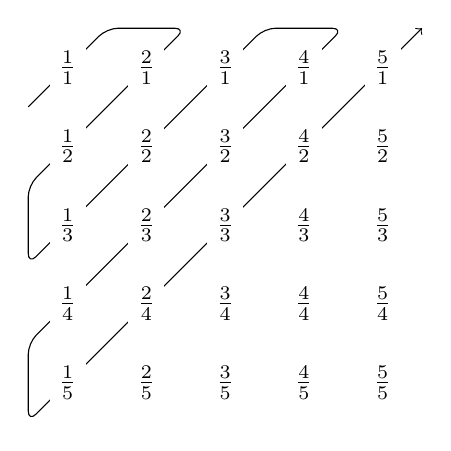
\begin{tikzpicture}
\draw[rounded corners, ->] (.5,-1.5) -- (1.5,-.5)
-- (2.5,-.5) -- (.5,-2.5)
-- (.5,-3.5) -- (3.5,-.5)
-- (4.5,-.5) -- (.5,-4.5)
-- (.5,-5.5) -- (5.5,-.5);
%
\node[fill=white] at (1,-1) {$\frac11$};
\node[fill=white] at (1,-2) {$\frac12$};
\node[fill=white] at (1,-3) {$\frac13$};
\node[fill=white] at (1,-4) {$\frac14$};
\node[fill=white] at (1,-5) {$\frac15$};
%
\node[fill=white] at (2,-1) {$\frac21$};
\node[fill=white] at (2,-2) {$\frac22$};
\node[fill=white] at (2,-3) {$\frac23$};
\node[fill=white] at (2,-4) {$\frac24$};
\node[fill=white] at (2,-5) {$\frac25$};
%
\node[fill=white] at (3,-1) {$\frac31$};
\node[fill=white] at (3,-2) {$\frac32$};
\node[fill=white] at (3,-3) {$\frac33$};
\node[fill=white] at (3,-4) {$\frac34$};
\node[fill=white] at (3,-5) {$\frac35$};
%
\node[fill=white] at (4,-1) {$\frac41$};
\node[fill=white] at (4,-2) {$\frac42$};
\node[fill=white] at (4,-3) {$\frac43$};
\node[fill=white] at (4,-4) {$\frac44$};
\node[fill=white] at (4,-5) {$\frac45$};
%
\node[fill=white] at (5,-1) {$\frac51$};
\node[fill=white] at (5,-2) {$\frac52$};
\node[fill=white] at (5,-3) {$\frac53$};
\node[fill=white] at (5,-4) {$\frac54$};
\node[fill=white] at (5,-5) {$\frac55$};
\end{tikzpicture}
\end{center}
Note that every positive rational number appears in this diagram. If $p$ and $q$ are positive integers, then $\frac{p}{q}$ appears in the $q$th row and $p$th column. Note also the shape of the path (following the direction of the arrow). We define a function $h$ from $\mathbb{Z}_{>0}$ to $\mathbb{Q}_{>0}$ by assigning a value of $h$ each time we encounter a rational number whose value we have not encountered before.

Thus, $h(1)=\frac11$, and $h(2)=\frac21$, and $h(3)=\frac12$, and $h(4)=\frac13$, but $h(5)\not=\frac22$, because we have already encountered the value $\frac22$ as $h(1)$. So, we skip over $\frac22$ and instead say $h(5)=\frac31$. Continuing, $h(6)=\frac41$ and $h(7)=\frac32$ and $h(8)=\frac23$ and $h(9)=\frac14$ and $h(10)=\frac15$. Note that $h(11)\not=\frac24$ because we have already encountered the value $\frac24$ when we said that $h(3)=\frac12$. So, instead, $h(11)=\frac51$, since we also need to skip over the values $\frac33=1$ and $\frac42=2$. Continue defining the outputs of $h$ in this way.

We see that $h$ is bijective by design. The function $h$ is surjective (every positive rational number appears in this diagram) and $h$ is injective (we skip over any rational number whose value we have already encountered).
\end{proof}
\begin{theorem}
The set $\mathbb{Q}$ is countable.
\end{theorem}
The proof of the previous theorem is left as an exercise. Prove this theorem using the previous theorem (that is, assume you have a bijection $h$ from $\mathbb{Z}_{>0}$ to $\mathbb{Q}_{>0}$) and use the ideas which made Exercise~\ref{exercise:Z-countable} successful.
\begin{exercise}
Prove the theorem above, that $\mathbb{Q}$ is countable.
\end{exercise}

\begin{theorem}
The set $\mathbb{R}$ is uncountable.
\end{theorem}
\begin{proof}
The proof we present is known as Cantor's Diagonalization Argument. To obtain a contradiction, suppose that $\mathbb{R}$ is countable. Then, $[0,1]$, which is a proper subset of $\mathbb{R}$ would also be countable. Since $[0,1]$ is not finite, then $[0,1]$ is countably infinite, thus there exists a bijection $f : \mathbb{Z}_{>0} \to [0,1]$.

Now, each element in $[0,1]$ has a decimal expansion of the form $0.d_1d_2d_3d_4d_5\dots$. For example, $\frac14 = 0.25000\dots$.
We will write out the decimal expansion of $f(1)$ as $0.d_{11}d_{12}d_{13}d_{14}d_{15}...$, and $f(2)$ as $0.d_{21}d_{22}d_{23}d_{24}d_{25}...$, and so on. More generally, $f(j)=0.d_{j1}d_{j2}d_{j3}d_{j4}d_{j5}\dots$, and thus $d_{jk} \in \{0,1,2,\dots,0\}$ is the $k$th digit in the decimal expansion of $h(j)$.

We will construct a real number $\ell$ whose decimal expansion we denote $\ell = 0.\ell_1\ell_2\ell_3\ell_4\ell_5\dots$ in the following manner:
\[
\ell_j =
\left\{
\begin{array}{ll}
8 & \text{if } d_{jj} = 5\\
5 & \text{if } d_{jj} \not=5.
\end{array}
\right.
\]
That is, if the first digit of $f(1)$ is a $5$ then the first digit of $\ell$ is $8$, and if the first digit of $f(1)$ is not a $5$ then the first digit of $\ell$ is $5$.
Likewise, if the second digit of $f(2)$ is a $5$ then the second digit of $\ell$ is $8$, and if the second digit of $f(2)$ is not a $5$ then the second digit of $\ell$ is $5$. In this manner, $\ell$ differs from $f(j)$ in the $j$th digit, so for all $j \in \mathbb{Z}_{>0}$, we have $\ell \not= f(j)$. But $\ell \in [0,1]$, so this proves that $f$ is not surjective, a contradiction to $f$ being bijective.
\end{proof}

The work of equicardinality involves the following: given two sets $A$ and $B$, define a function from $A$ to $B$ that is bijective. An important intuition-building exercise is to consider when $A=\mathbb{R}$ and $B=\mathbb{R}$:
\begin{exercise}
In this exercise, there is not \emph{one} correct answer:
\begin{enumerate}
\item Define a function from $\mathbb{R}$ to $\mathbb{R}$ which is injective but not surjective.
\item Define a function from $\mathbb{R}$ to $\mathbb{R}$ which is surjective but not injective.
\item Define a function from $\mathbb{R}$ to $\mathbb{R}$ which is injective and surjective.
\item Define a function from $\mathbb{R}$ to $\mathbb{R}$ which is neither injective nor surjective.
\end{enumerate}
\end{exercise}

\begin{theorem}
The subsets $A=[3,7]$ and $B=[5,20]$ of $\mathbb{R}$ are equicardinal.
\end{theorem}
First, note that $3$ is the smallest input and $5$ is the smallest output. Second, note $7$ is the largest input, while $20$ is the largest output. One can write $y-5=\frac{15}{4}(x-3)$ as an equation for the line going through the points $(3,5)$ and $(7,20)$. This was how we determined the rule for the function $h$ in the proof to be $h(x)= \frac{15}{4}(x-3)+5$. Now, we prove the theorem:
\begin{proof}
Let $h : [3,7] \to [5,20]$ be the function defined by the rule
$h(x)=\frac{15}{4}(x-3)+5$.

First we ensure that $[5,20]$ as stated for the domain is accurate. In other words, we would have a ``problem'' if the value of $\frac{15}{4}(x-3)+5$ is \emph{not} between $5$ and $20$ for any $x$-value between $3$ and $7$.
\begin{itemize}
    \item Note that $h(3)=\frac{15}{4}(3-3)+5=0+5=5$.
    \item Note that $h(7)=\frac{15}{4}(7-3)+5=15+5=20$.
    \item Note $h'(x)=\frac{15}{4}$. Since $h'(x) > 0$ for all $x \in [3,7]$, the function $h$ is increasing on this interval, and with $h(3)=5$ and $h(7)=20$, this shows that $h(x)$ is in $[5,20]$ for all $x \in [3,7]$.
\end{itemize}
Therefore, the stated codomain of $[5,20]$ is acceptable, following the requirement mentioned in Warning~\ref{warning:in-codomain}.

To prove $h$ is injective, let $a,b \in [3,7]$ both be arbitrary. Suppose $h(a)=h(b)$.
Then $\frac{15}{4}(a-3)+5=\frac{15}{4}(b-3)+5$.
So $\frac{15}{4}(a-3)=\frac{15}{4}(b-3)$.
Multiplying both sides by $\frac{4}{15}$, we learn $a-3=b-3$.
Therefore $a=b$, and $h$ is injective.

To prove $h$ is surjective, let $z \in [5,20]$ be arbitrary. We want to prove that there exists $m \in [3,7]$ such that $h(m)=z$.
\vskip2pt
\begin{framed}
\noindent
Scratch work. Leave everything in this box out of the proof. Want $h(m)=z$. In other words, want $\frac{15}{4}(m-3)+5=z$. Solving for $m$, we get $m=3+\frac{4}{15}(z-5)$.
\end{framed}
\noindent Let $m=3+\frac{4}{15}(z-5)$. We will prove $m \in [3,7]$ and we will prove $h(m)=z$.
\begin{itemize}
    \item To prove $m \in [3,7]$, note $5 \leq z \leq 20$. By subtracting, $0 \leq z-5 \leq 15$. By multiplication (by a positive), $0 \leq \frac{4}{15}(z-5) \leq 4$. By addition, $3 \leq 3+\frac{4}{15}(z-5)\leq 7$. We replace the quantity in the middle with the definition of $m$, so $3 \leq m \leq 7$, which proves $m \in [3,7]$.
    \item  To prove $h(m)=z$, note 
    \begin{align*}
    h(m)
    &=\textstyle\frac{15}{4}(m-3)+5\\
    &=\textstyle\frac{15}{4}([3+\frac{4}{15}(z-5)]-3)+5\\
    &=\textstyle\frac{15}{4}\cdot \frac{4}{15}(z-5)+5\\
    &=(z-5)+5\\
    &=z,
    \end{align*}
    and since $m \in [3,7]$ and $h(m)=z$, we have proved that there exists $m \in A$ such that $h(m)=z$. Since the choice of $z \in B$ was arbitrary, $h$ is surjective.
\end{itemize}
Since $h$ is bijective, $[3,7]$ and $[5,20]$ are equicardinal.
\end{proof}

Given $A=[3,7]$ and $B=[5,20]$, what was the intuition behind using the rule $h(x)= \frac{15}{4}(x-3)+5$? Both $A$ and $B$ are subsets of $\mathbb{R}$, but since $A$ is the domain, imagine thickening the portion of the $x$-axis where $3 \leq x \leq 7$. Similarly, thicken the portion of the $y$-axis where $5 \leq y \leq 20$. The line through the points $(3,5)$ and $(7,20)$ would be the graph of a bijective function from $\mathbb{R}$ to $\mathbb{R}$. An equation for that line is $y-5=\frac{15}{4}(x-3)$ in point-slope form. The line \emph{segment} with endpoints $(3,5)$ and $(7,20)$ would be the graph of a bijective function from $A$ to $B$. 

\begin{exercise}
Let $A$, $B$, $C$, and $D$ be sets. Suppose $A$ and $C$ have the same cardinality. Suppose $B$ and $D$ have the same cardinality. Prove $A \times B$ has the same cardinality as $C \times D$.%\quad\quad\href{https://www.sharelatex.com/project/5a073823a150fe764ab07b68}{{\color{red}[key]}}
\end{exercise}

\begin{exercise}
Let $A$ and $B$ be sets. Prove that if $A$ and $B$ have the same cardinality, then $P(A)$ and $P(B)$ have the same cardinality.%\quad\quad\href{https://www.sharelatex.com/project/5a073848a150fe764ab07b6c}{{\color{red}[key]}}
\end{exercise}

\begin{exercise}
Let $f : X \to Y$ be an injective function. Prove that $X$ and $f(X)$ have the same cardinality.%\quad\quad\href{https://www.sharelatex.com/project/5a073893a150fe764ab07b88}{{\color{red}[key]}}
\end{exercise}

\begin{exercise}
Prove that $(3,7)$ and $(5,12)$ have the same cardinality.%\quad\quad\href{https://www.sharelatex.com/project/5a073862a150fe764ab07b7a}{{\color{red}[key]}}
\end{exercise}

\begin{exercise}
Prove that the set $[2,7] = \{a \in \mathbb{R} : 2 \leq a \leq 7\}$ and the set $[3,14]=\{p \in \mathbb{R} : 3 \leq p \leq 14\}$ are equicardinal.
\end{exercise}

% challenging

\begin{exercise}
Prove the relation ``$A$ has the same cardinality as $B$'' is an equivalence relation on sets.
\end{exercise}

\begin{exercise}
Prove: if $B$ is countable and $A \subseteq B$, then $A$ is countable. %\quad\quad\href{https://www.sharelatex.com/project/5a07358aa150fe764ab07abe}{{\color{red}[key]}}
\end{exercise}

\begin{exercise}
Prove: if $A$ and $B$ are countable, then $A \cap B$ is countable. (You cannot assume that $A$ and $B$ are disjoint.) For good practice, prove this statement without using the previous exercise.% \quad\quad\href{https://www.sharelatex.com/project/5a0735b2a150fe764ab07ac4}{{\color{red}[key]}}
\end{exercise}

\section{Induction}

Let $P(n)$ be a predicate. The traditional way (Method~\ref{method:proving-forall}) to prove \fbox{$\forall k \in \mathbb{Z}_{>0}$, $P(k)$} is to select $k \in \mathbb{Z}_{>0}$ arbitrarily and work to prove $P(k)$. Sometimes, one can get stuck trying this traditional proof method. The method of induction provides an alternate means for proving $P(k)$ is true for all $k \in \mathbb{Z}_{>0}$.

\begin{bmethod}{Proof by induction}{induction}
To prove $\forall n \in \mathbb{Z}_{>0}$, $P(n)$ by induction, one must prove:
\begin{itemize}
\item \defn{base case}: prove $P(1)$
\item \defn{inductive step}: prove $\forall k \in \mathbb{Z}_{>0}$, if $P(k)$ then $P(k+1)$
\end{itemize}
\end{bmethod}

A proof by induction\index{induction}\index{proof by induction} consists of the proof writer filling in the details for dotted arrows in Figure~\ref{figure:induction-justification-flowchart}, taking the defined $P(n)$ and establishing $P(1)$ is true (\defn{base case}\index{base case}), and  \fbox{$\forall k \in \mathbb{Z}_{>0}$, if $P(k)$ then $P(k+1)$} is true (\defn{inductive step}\index{inductive step}). If those are established, the generic part of the argument (called the \defn{Principle of Mathematical Induction}\index{Principle of Mathematical Induction}) is the bottom half of the flowchart below, and is not written out in standard proofs, because the argument is always the same.
\begin{center}
\begin{figure}
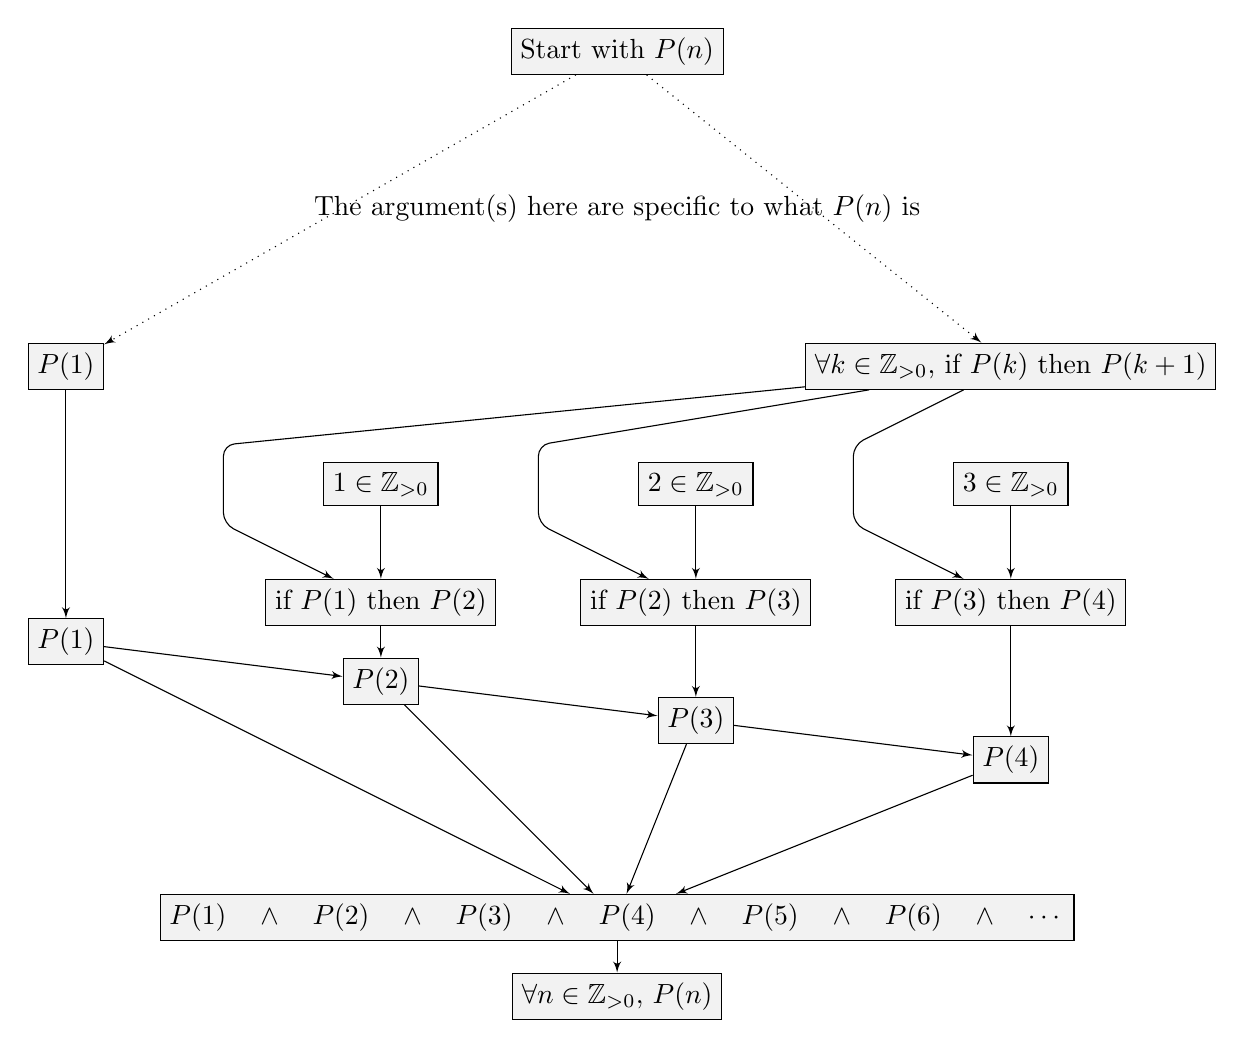
\begin{tikzpicture}
\node [block] (start) at (7,4) {Start with $P(n)$};

\node [block] (base) at (0,0) {$P(1)$};
\node [block] (ind) at (12,0) {$\forall k \in \mathbb{Z}_{>0}$, if $P(k)$ then $P(k+1)$};

\path [line, dotted] (start) -- (base);
\path [line, dotted] (start) -- (ind);

\node at (7,2) {The argument(s) here are specific to what $P(n)$ is};

\node [block] (z1) at (4,-1.5) {$1 \in \mathbb{Z}_{>0}$};
\node [block] (z2) at (8,-1.5) {$2 \in \mathbb{Z}_{>0}$};
\node [block] (z3) at (12,-1.5) {$3 \in \mathbb{Z}_{>0}$};
%\node [block] (z4) at (16,-1.5) {$4 \in \mathbb{Z}_{>0}$};
%\node [block] (z5) at (20,-1.5) {$5 \in \mathbb{Z}_{>0}$};

\node [block] (if1) at (4,-3) {if $P(1)$ then $P(2)$};
\node [block] (if2) at (8,-3) {if $P(2)$ then $P(3)$};
\node [block] (if3) at (12,-3) {if $P(3)$ then $P(4)$};
%\node [block] (if4) at (16,-3) {if $P(4)$ then $P(5)$};
%\node [block] (if5) at (20,-3) {if $P(5)$ then $P(6)$};

\path [line, rounded corners] (ind) -- (2,-1) -- (2,-2.0) -- (if1);
\path [line, rounded corners] (ind) -- (6,-1) -- (6,-2.0) -- (if2);
\path [line, rounded corners] (ind) -- (10,-1) -- (10,-2.0) -- (if3);
%\path [line, rounded corners] (ind) -- (14,-1) -- (14,-2.0) -- (if4);
%\path [line, rounded corners] (ind) -- (18,-1) -- (18,-2.0) -- (if5);

\path [line] (z1) -- (if1);
\path [line] (z2) -- (if2);
\path [line] (z3) -- (if3);
%\path [line] (z4) -- (if4);
%\path [line] (z5) -- (if5);

\node [block] (p1) at (0,-3.5) {$P(1)$};
\node [block] (p2) at (4,-4.0) {$P(2)$};
\node [block] (p3) at (8,-4.5) {$P(3)$};
\node [block] (p4) at (12,-5.0) {$P(4)$};
%\node [block] (p5) at (16,-5.5) {$P(5)$};
%\node [block] (p6) at (20,-6.0) {$P(6)$};

\path [line] (base) -- (p1);
\path [line] (p1) -- (p2); \path [line] (if1) -- (p2);
\path [line] (p2) -- (p3); \path [line] (if2) -- (p3);
\path [line] (p3) -- (p4); \path [line] (if3) -- (p4);
%\path [line] (p4) -- (p5); \path [line] (if4) -- (p5);
%\path [line] (p5) -- (p6); \path [line] (if5) -- (p6);

\node [block] (and) at (7,-7) {$P(1) \quad\wedge\quad P(2) \quad\wedge\quad P(3) \quad\wedge\quad P(4) \quad\wedge\quad P(5) \quad\wedge\quad P(6) \quad\wedge\quad \cdots $};

\path [line] (p1) -- (and);
\path [line] (p2) -- (and);
\path [line] (p3) -- (and);
\path [line] (p4) -- (and);
%\path [line] (p5) -- (and);
%\path [line] (p6) -- (and);

\node [block] (final) at (7,-8) {$\forall n \in \mathbb{Z}_{>0},\,P(n)$};

\path [line] (and) -- (final);

\end{tikzpicture}
\caption{Justification of proof by induction}\label{figure:induction-justification-flowchart}
\end{figure}
\end{center}

Let us consider an example:
\begin{theorem}
The identity $\displaystyle\frac{n(n+1)}{2}= \sum_{j=1}^n j$ holds for all $n \in \mathbb{Z}_{>0}$.
\end{theorem}
\begin{proof}
We provide more detail than is typical, as this is our first induction proof. First, note that $P(n)$ is the predicate $\displaystyle\frac{n(n+1)}{2}= \sum_{j=1}^n j$.

For the base case, we need to prove $P(1)$. In other words, we need to prove $\displaystyle\frac{1(1+1)}{2}= \sum_{j=1}^1 j$. Note that $\sum_{j=1}1 j = 1 = \frac22 = \frac{1(1+1)}{2}$, so the base case is proved.

The inductive step is to prove $\forall k \in \mathbb{Z}_{>0}$, if $P(k)$ then $P(k+1)$. As we traditionally would do following Method~\ref{method:proving-forall}, we let $k \in \mathbb{Z}_{>0}$ be arbitrary. We want to prove if $P(k)$ then $P(k+1)$. So, assume $\displaystyle\frac{k(k+1)}{2}= \sum_{j=1}^k j$. We want to prove $\displaystyle\frac{(k+1)((k+1)+1)}{2}= \sum_{j=1}^{k+1} j$.

How does the statement that we want to prove, namely $\displaystyle\frac{(k+1)((k+1)+1)}{2}= \sum_{j=1}^{k+1} j$, relate to the statement we assumed was true, namely $\displaystyle\frac{k(k+1)}{2}= \sum_{j=1}^k j$? Notice that $\displaystyle \sum_{j=1}^{k+1} j = (k+1)+\sum_{j=1}^{k} j$, and note that $\sum_{j=1}^{k} j$ can be replaced with $\frac{k(k+1)}{2}$. So,
\begin{align*}
\sum_{j=1}^{k+1} 
&= \left[ \sum_{j=1}^k j \right] + (k+1)\\
&= \frac{k(k+1)}{2} + (k+1)\\
&= \frac{k^2+k}{2} + \frac{2k+2}{2}\\
&= \frac{k^2+3k+2}{2}\\
&= \frac{(k+1)(k+2)}{2}\\
&= \frac{(k+1)((k+1)+1)}{2},
\end{align*}
and thus the inductive step is proved.

Using mathematical induction, for all $n \in \mathbb{Z}_{>0}$, we have $\sum_{j=1}^n j = \frac{n(n+1)}{2}$.
\end{proof}
For a shortened version of the proof:
\begin{proof}
We prove by induction. For the base case, $\sum_{j=1}1 j = 1 = \frac22 = \frac{1(1+1)}{2}$. For the inductive step, $k \in \mathbb{Z}_{>0}$ be arbitrary, and assume $\displaystyle\frac{k(k+1)}{2}= \sum_{j=1}^k j$. So,
\[
\sum_{j=1}^{k+1} j
= \left[ \sum_{j=1}^k j \right] + (k+1)
= \frac{k(k+1)}{2} + (k+1)
= \frac{(k+1)(k+2)}{2}.
\]
\end{proof}
When we talk about \defn{mathematical induction} or \defn{induction}, we mean this proof method. The word ``induction'' is used in everyday language to mean ``making a conclusion that (vaguely) seems likely to be true'' based on repeated observation. We do not mean this at all.

In the proof above, $P(k)$ is called the \defn{inductive hypothesis}\index{inductive hypothesis}. In our specific example, the inductive hypothesis was the assumed statement $\frac{k(k+1)}{2}= \sum_{j=1}^k j$.

\begin{theorem}\label{theorem:induction-divides}
For all positive integers $n$, the integer $3$ divides $n^3+2n+9$.
\end{theorem}
Before proving Theorem~\ref{theorem:induction-divides}, some comments are in order. Note that $P(n)$ is the predicate ``$3$ divides $n^3+2n+9$.''
\begin{bwarning}{}{}
If you use $P(n)$ for a predicate, but $P(n)$ includes a function $p$, do not say that $p(n)$ is true!
\end{bwarning}
\begin{example}
We will not say that $P(n)$ is $n^3+2n+9$. If we'd like to, we can define a function $p : \mathbb{Z}_{>0} \to \mathbb{Z}$ by saying that $p(n)=n^3+2n+9$, but if we do so, let us not confuse $P(n)$ with $p(n)$. Here, $p(n)$ is a function and $P(n)$, following the notation from earlier, is a predicate. In fact, $P(n)$ is the statement that $3$ divides the number $p(n)$. While we could speak of $P(5)$ being true, we could not speak of $p(5)$ being true, since $p(5)$ is just a number. Similarly, we cannot talk about $p(n)$ being true or false.
\end{example}
We now prove Theorem~\ref{theorem:induction-divides}.
\begin{proof}
For our base case, we need to prove $3$ divides $1^3+2(1)+9$. Let $c = 4 \in \mathbb{Z}$. Then $3c = 3 \cdot 4 = 12 = 1+2+9=1^3+2(1)+9$. Since $c \in \mathbb{Z}$ and $3c=1^3+2(1)+9$, we have proved $3$ divides $1^3+2(1)+9$.

For the inductive step, let $k \in \mathbb{Z}_{>0}$ be arbitrary. Suppose $3$ divides the integer $k^3+2k+9$. We want to show $3$ divides $(k+1)^3+2(k+1)+9$. Since $3$ divides $k^3+2k+9$, there exists an integer $w$ such that $3w =k^3+2k+9$. Let $r = w+k^2+k+1$. Then,
\begin{align*}
(k+1)^3+2(k+1)+9
&= k^3+3k^2+3k+1+2k+2+9\\
&= k^3+2k+9+3k^2+3k+3\\
&= 3w + 3k^2+3k+3\\
&= 3(w+k^2+k+1)\\
&= 3r.
\end{align*}
Since $r \in \mathbb{Z}$ and $3r=(k+1)^3+2(k+1)+9$, this proves that $3$ divides $(k+1)^3+2(k+1)+9$, completing the inductive step.
\end{proof}

\begin{exercise}
Prove: for all $n \in \mathbb{Z}_{>0}$, the equality $\displaystyle \sum_{i=1}^n i^2 = \frac{n(n+1)(2n+1)}{6}$ holds.
\end{exercise}

\begin{exercise}
Prove: $n! < n^n$ for all integers $n > 1$.
\end{exercise}

\begin{exercise}
Prove $1+3+5+\cdots (2n-1) = n^2$ for all $n \in \mathbb{Z}_{>0}$.\quad\quad\href{https://www.sharelatex.com/project/5a0736a8a150fe764ab07afb}{{\color{red}[key]}}
\end{exercise}

\begin{exercise}
Prove for all $n > 0$ which are integer, one has 
\[ \sum_{j=1}^n \frac{1}{j(j+1)} = \frac{n}{n+1} \]
\quad\quad\href{https://www.sharelatex.com/project/5a073648a150fe764ab07aed}{{\color{red}[key]}}
\end{exercise}

\begin{exercise}
Suppose $f : \mathbb{R} \to \mathbb{R}$ satisfies $f(x+y)=f(x)+f(y)$ for all real numbers $x$ and $y$. Fix a real number $s$.  Prove for all $n \in \mathbb{Z}_{>0}$, the equation $f(ns)=n\,f(s)$ holds.\quad\quad\href{https://www.sharelatex.com/project/5a073787a150fe764ab07b4c}{{\color{red}[key]}}
\end{exercise}

\begin{exercise}
Prove $5$ divides $6^n+4$ for all $n \in \mathbb{Z}_{>0}$.\quad\quad\href{https://www.sharelatex.com/read/jqnhvtfzgqsp}{{\color{red}[key]}}
\end{exercise}

\begin{exercise}
Prove $4$ divides $n(n+2)$ if $n$ is any even positive integer. (Hint: create for yourself a modified type of mathematical induction) \quad\quad\href{https://www.sharelatex.com/read/hjkgbqfwdqjj}{{\color{red}[key]}}
\end{exercise}

\begin{exercise}
Prove $8$ divides $3^{2k}-1$ for all $k \in \mathbb{Z}_{>0}$. \quad\quad\href{https://www.sharelatex.com/read/ntwyhgyqzhdt}{{\color{red}[key]}}
\end{exercise}

\begin{exercise}
Prove for every positive integer $n$, the integer $9$ divides $n^3+(n+1)^3+(n+2)^3$.
\end{exercise}

\subsection{Strong induction}

Let $P(n)$ be a predicate. Perhaps the traditional way (Method~\ref{method:proving-forall}) to prove $\forall k \in \mathbb{Z}_{>0}$, $P(k)$ fails to work, and perhaps the method of mathematical induction just introduced in the previous section also fails to work. Proof by strong induction\index{strong induction}\index{proof by strong induction} provides yet another means for proving $P(k)$ is true for all $k \in \mathbb{Z}_{>0}$.

\begin{bmethod}{Proof by strong induction}{strong-induction}
To prove $\forall n \in \mathbb{Z}_{>0}$, $P(n)$ using strong induction, one must prove:
\begin{itemize}
\item \defn{base case}: prove $P(1)$
\item \defn{inductive step}: prove for all $k \in \mathbb{Z}_{>0}$, if $P(1) \wedge P(2) \wedge \dots \wedge P(k)$, then $P(k+1)$.
\end{itemize}
Here, the \defn{inductive hypothesis} is $P(1) \wedge P(2) \wedge \dots \wedge P(k)$, where as earlier, the inductive hypothesis (in standard induction) was just $P(k)$.
\end{bmethod}

Before looking at an example, we will need a definition.
\begin{bdefinition}{}{}
Let $f_n$ denote the \defn{Fibonacci sequence}\index{Fibonacci sequence}, defined by
\begin{align*}
f_1 &= 1\\
f_2 &= 1\\
f_n &= f_{n-1}+f_{n-2}, \quad \text{if } n > 2.
\end{align*}
\end{bdefinition}

\begin{theorem}
If $f_n$ denotes the $n$th Fibonacci number, then for all $n \in \mathbb{Z}_{>0}$, the equation $f_{n+6}=4f_{n+3}+f_n$ is true.
\end{theorem}
\begin{proof}
Let $P(n)$ be the predicate $f_{n+6}=4f_{n+3}+f_n$. We will proceed with a proof by strong induction.

For the base case, we want to show that $P(1)$ is true. Since $f_7=13$ and $4f_4+f_1=4(3)+1=13$, we see that $P(1)$ holds.

For the inductive step, let $k \in \mathbb{Z}_{>0}$ be arbitrary. Suppose that $P(1)$, \dots, and $P(k)$ are all true (the inductive hypothesis). We want to show that $P(k+1)$ is true. In other words, we want to show that $f_{k+7}=4f_{k+4}+f_{k+1}$ holds. We have
\begin{align*}
f_{k+7} 
&= f_{k+6} + f_{k+5} \\
&= (4f_{k+3}+f_k) + (4f_{k+2}+f_{k-1}) \\
&= 4(f_{k+3}+f_{k+2})+(f_k) f_{k-1}) \\
&= 4f_{k+4} + f_{k+1},
\end{align*}
where the first and last equalities come from the recursive definition of the Fibonacci sequence, and the second equation are from $P(k-1)$ and $P(k)$, which came from the inductive hypotheses.
\end{proof}

\begin{exercise}
Let $f_0=1, f_1=1$, and if $n>1$, then $f_n=f_{n-1}+f_{n-2}$. Let $\phi = \frac12(1+\sqrt{5})$. Prove that $f_n \leq \phi^n$ for all $n \in \mathbb{Z}_{\geq 0}$.\quad\quad\href{https://www.sharelatex.com/read/vxjjxmvmgjmj}{{\color{red}[key]}}
\end{exercise}

\begin{exercise}
Let $g : \mathbb{Z}_{>0} \to \mathbb{Z}$ be the function defined by the rule
\[
g(n) = \left\{
\begin{array}{ll}
1 & \text{if } n=1,\\
5 & \text{if } n=2,\\
5g(n-1)-6g(n-2) & \text{if } n > 2.
\end{array}
\right.
\]
Prove: $g(n)=3^n-2^n$ for all $n \in \mathbb{Z}_{>0}$.
\end{exercise}

%\section{Well-ordering principle}
%
%This section is not yet written, but is included for consistent numbering with future editions.
%This section will discuss the well-ordering principle\index{well-ordering principle}.
%
%\section{Superlatives}
%
%This section is not yet written, but is included for consistent numbering with future editions.
%This section will discuss working with superlatives\index{superlative} such as minimal\index{minimal}, maximal\index{maxima}, smallest\index{smallest}, and largest\index{largest}. Proofs requiring manipulation of sentences involving smallest or largest (by set inclusion, etc.) will be discussed.
%
%\section{Equality for real numbers}
%
%This section is not yet written, but is included for consistent numbering with future editions.
%This section will discuss trichotomy\index{trichotomy} and techniques for proving two real numbers are equal.
%
%\section{Additional proofs of existence}
%
%This section is not yet written, but is included for consistent numbering with future editions.
%This section will discuss proving existentially-quantified statements without naming the constructed object. This section will discuss non-constructive\index{non-constructive} proofs of existence.
%
%\section{Literary devices}
%
%This section is not yet written, but is included for consistent numbering with future editions.
%This section will discuss the literary devices ``a priori''\index{a priori} and ``up to''\index{up to} as used in mathematical proofs.

\chapter{Counting}

This chapter investigates the principles of mathematical counting. The chapter largely does not rely on much of the content of the previous chapters, though there is some language of sets and functions which will appear. The word ``counting'' makes it sound like we will walk through ``one, two, three, four.'' Don't worry: our counting problems will be more interesting than that.

\section{The Product and Sum Rules}\label{section:basic-counting}

The Product Rule does not always apply, but when it does, it takes a more complex task (which we call a procedure) and counts how many ways there are to do the procedure in terms of simpler tasks:
\begin{bmethod}{Product Rule}{product-rule}
Suppose that a procedure can be broken down into a sequence of two independent tasks. If there are $n_1$ ways to do the first task and $n_2$ ways to do the second task, then there are $n_1n_2$ ways to do the procedure.
\end{bmethod}

To justify this rule which claims that there are $n_1n_2$ ways to do the procedure, consider the following set up. Let $F$ be a set consisting of $n_1$ elements: the elements of $F$ are precisely the $n_1$ ways to do the first task. Let $S$ be a set consisting of $n_2$ elements: the elements of $S$ are precisely the $n_2$ ways of doing the second task. The procedure is done by selecting one of the $n_1$ options for the first task, followed by selecting one of the $n_2$ options for the second task. Then $|F \times S| = |F| \times |S|$, and each element of $F \times S$ is an ordered pair, which represents a different way to do the procedure.

When does the Product Rule apply? The Product Rule applies when there are two \emph{independent} tasks, and \emph{both} tasks must be performed.

\begin{example}\label{example:letter-number}
In a certain psychology experiment, to protect the identities of the subjects, each participant is to be identified only using a pairing of a letter and a number. How many possible participant identifiers are there?

The procedure of determining a participant identifier requires a first task of choosing one of $n_1=26$ letters, and a second task of choosing one of $n_2=10$ digits (from $0$ through $9$, inclusive). The procedure is incomplete just doing one task or the other: both tasks must be completed. Thus, the total number of participant identifiers is $260$.
\end{example}

\begin{example}\label{example:menu-del-dia}
In Spain, a popular way to do lunch is called the men\'u del dia. A typical restaurant's men\'u del dia will consist of the diner selecting exactly one choice from the ``first plates'' list, exactly one item from the ``second plates'' list, and one item from the ``desserts'' list, with the price fixed to be constant (independent of the choices made). Suppose one restaurant offers the following choices:
First plates are sopa castellana, sopa de pescado, or djudias blancas.
Second plates are cordero asado, pescadilla a la romana, chuleta de aguja, or trucha ala navarra.
Dessert choices are crema catalana or helado.
%https://www.tripadvisor.com.sg/LocationPhotoDirectLink-g1079423-d3673593-i53345314-Restaurante_San_Marcos-Barraco_Province_of_Avila_Castile_and_Leon.html

How many different meals can be made? Since there are $3$ choices for first plate, $4$ choices for second plate, and $2$ choices for desert, there are $3 \cdot 4 \cdot 2 = 24$ possible meals. (That is, $24$ visitors to this restaurant can have unique dining experiences. We have avoided using the word ``combination'' which has a specific meaning in a future section.)
\end{example}

In cases where the Product Rule does not apply, the Sum Rule might apply. Like the Product Rule, the Sum Rule takes a more complex task (which we call a procedure) and counts how many ways to do this procedure in terms of simpler tasks.
\begin{bmethod}{Sum Rule}{sum-rule}
Suppose a procedure is done by picking exactly one of two tasks to do. If there are $n_1$ ways to do the first task and $n_2$ ways to do the second task, then there are $n_1+n_2$ ways to do the procedure.
\end{bmethod}
To justify this rule which claims that there are $n_1+n_2$ ways to do the procedure, consider the following set up. Let $F$ be a set consisting of $n_1$ elements: the elements of $F$ are precisely the $n_1$ ways to do the first task. Let $S$ be a set consisting of $n_2$ elements: the elements of $S$ are precisely the $n_2$ ways of doing the second task. If there are truly $n_1$ ways to do the first task and $n_2$ ways to do the second task, then $F \cup S$ represents the set of ways to do exactly one task, assuming $F$ and $S$ are disjoint. That is, if $F \cap S = \emptyset$, then $|F \cup S| = |F| + |S|$.

When does the Sum Rule apply? The Sum Rule applies when there are two tasks, but only \emph{one} of the two tasks is performed.
\begin{example}
At a restaurant downtown, any choice of dinner place comes with either soup or salad (but not both). There are $3$ soup selections, and $2$ salad choices. How many possible accompaniments (without the up-charge of both) are there to a dinner? Is the correct answer $5$ or $6$?

There are three possible ways to complete the first task (choose one of the three soups). There are two possible ways to finish the second task (choose one of the two salads). For this particular thought experiment, the procedure is complete by doing \emph{one} of the two tasks. Therefore, there are $5$ ways to complete the procedure.
\end{example}

\begin{example}
At another restaurant downtown, any choice of dinner place comes with both soup and salad. There are $3$ soup selections, and $2$ salad choices. How many possible accompaniments are there to a dinner? Is the correct answer $5$ or $6$?

There are three possible ways to complete the first task (choose one of the three soups). There are two possible ways to finish the second task (choose one of the two salads). For this particular thought experiment, the procedure is complete by doing \emph{both} of the tasks. Therefore, there are $6$ ways to complete the procedure.
\end{example}

\begin{bwarning}{Do not confuse the Product Rule and the Sum Rule}{}
Do not apply the Sum Rule when only the Product Rule can be used.
Do not apply the Product Rule when only the Sum Rule can be used.
\end{bwarning}

\begin{bmethod}{Product Rule versus Sum Rule}{product-vs-sum}
How can you stop confusing the Product Rule and the Sum Rule? Take the [larger] procedure and identify two smaller tasks. Do you have to complete \emph{both} tasks to do the procedure, or are you \emph{only} allowed to do one task to do the procedure? If you must do both tasks, you probably need to use the Product Rule.
\vskip6pt
Consider this another way: imagine that you completed only \emph{one} of the two tasks. If the procedure would be incomplete in this situation, it is probably because both tasks need to be completed, and the Product Rule probably applies.
\end{bmethod}
As an example of Method~\ref{method:product-vs-sum}, let us refer back to Example~\ref{example:letter-number}. What would happen if only one procedure were complete? Then, we'd have a choice of a letter (such as picking ``W'') but if we stopped there, we could not have completed the procedure of creating a participant identifier.

\begin{example}\label{example:binary-string-n}
A binary string is a string consisting only of $0$s and $1$s. For instance, $10111$ and $0101101010001$ are examples of binary strings. The first example is a binary string of length $5$ while the second example is a binary string of length $13$. How many binary strings of length $13$ are there?

We will answer the more general question of how many binary strings of length $n$ there are. To make our argument, we focus on the number of binary strings of length $3$. Imagine that there are four boxes, and in each box, we must make the choice of either a $0$ or a $1$. Imagine repeating this procedure in every way possible. We would discover each of the binary strings of length $3$.

There are four tasks. The first task is choosing a $0$ or a $1$ for the first location. The second task is choosing a $0$ or a $1$ for the second location. The third task is choosing a $0$ or a $1$ for the third location. All three tasks are similar (choosing a $0$ or a $1$), and each task has two ways to complete it.

Does the Product Rule apply or does the Sum Rule apply? That is, is the final answer $2\cdot2\cdot2$ or $2+2+2$? Use Method~\ref{method:product-vs-sum} to determine the answer. To get a binary string of length $3$, notice that all three tasks must be completed. Thus, there are $2^3$ binary strings of length $4$. Convince yourself for sure by writing out all $8$ binary strings of length $3$. More generally, there are $2^n$ binary strings of length $n$.
\end{example}

\begin{example}\label{example:binary5or6}
How many binary strings are there of length $5$ or $6$? Recall that in Example~\ref{example:binary-string-n}, we determined that there are $2^n$ binary strings of length $n$.

In this problem, we should think of the [large] procedure as ``making a binary string whose length is either $5$ or $6$.'' While there are several ways to think of how to do the procedure, to connect this to the work we have already done, suppose there are two tasks. The first task is to ``make a binary string of length $5$'' and the second is to ``make a binary string of length $6$.'' Then, to complete the procedure, we must complete exactly one of the two tasks, so the Sum Rule applies. Therefore, the total number of binary strings of length $5$ or $6$ is exactly $2^5+2^6$.

Presented differently, there are $2\cdot2\cdot2\cdot2\cdot2 + 2\cdot2\cdot2\cdot2\cdot2\cdot2$ strings. Written this way, we can see all the uses of the Product Rule and the one use of the Sum Rule.
\end{example}

\begin{btheorem}{Inclusion-Exclusion Principle}{}
If $A$ is a finite set and $B$ is a finite set, then $|A \cup B| = |A| + |B| - |A \cap B|$.
\end{btheorem}
\begin{bwarning}{}{}
The Inclusion-Exclusion Principle is a theorem that applies to finite sets only. The theorem does not apply if $A$ is infinite or if $B$ is infinite. If any set you encounter is infinite and the question deals with making equal the sizes of given sets, instead of using the Inclusion-Exclusion Principle (which does not apply), it is likely that the methods in Section~\ref{section:cardinality} on cardinality apply.
\end{bwarning}
The purpose of subtracting $|A \cap B|$ is to address the double-counting that occurs when considering $|A| + |B|$.

\begin{example}
How many two-digit numbers have exactly one $7$ as a digit? Let $A$ be the set of all two-digit numbers where the starting digit is a $7$. Let $B$ be the set of all two-digit numbers where the ending digit is a $7$. Then $|A|=10$ and $|B|=10$. What is $|A \cap B|$? This is the number of two-digit numbers where the starting digit is a $7$ and the ending digit is a $7$. There is exactly one number that is described like this, namely $77$. Thus $|A \cap B|=1$. Therefore, the number of two-digit numbers which have exactly one $7$ as a digit is exactly $10+10-1$.
\end{example}

\begin{btheorem}{Inclusion-exclusion principle for three sets}{}
If $A$, $B$, and $C$ are all finite sets, then $|A \cup B| = |A| + |B| + |C| - |A \cap B| - |A \cap C| - |B \cap C| + |A \cap B \cap C|$.
\end{btheorem}

\begin{exercise}
In a standard $8 \times 8$ chessboard, a rook may move any number of spaces horizontally or vertically, with the restriction that the rook must stop at the first square to capture a piece of the opposite color. Assuming that a chessboard only contains one black rook and one white rook (and no other pieces), how many chessboard configurations are there where neither rook is in danger of being captured in the next move by the other rook? \end{exercise}

\begin{exercise}
Now consider using an $n \times n$ chessboard. Assuming that a chessboard only contains one black rook and one white rook (and no other pieces), how many $n \times n$ chessboard configurations are there where neither rook is in danger of being captured in the next move by the other rook?
\end{exercise}

\begin{exercise}
A banking website requires customers using online banking to choose a password, whose length must be at least $8$ characters and at most $20$ characters. For simplicity, let's say that passwords are restricted to using the $2 \cdot 26$ upper/lowercase letters and the $10$ numerical digits. (So, no special characters like the ``at symbol'' are allowed, to make sure that things aren't too complicated.) If a valid password must contain both numbers and letters, then how many possible passwords are there?
\end{exercise}

\begin{exercise}
A hexadecimal digit is a character which is either one of the 10 numeric digits or one of the first six letters (A through F) in the alphabet. For example, 19A0C0BE32D6FF21AB3 is a hexadecimal string. A wifi password must be a string of either 10, 26, or 58 hexadecimal digits. How many different passwords are possible?%\quad\quad\href{https://www.sharelatex.com/read/ypxvvtddbmss}{{\color{red}[key]}}
\end{exercise}

\section{Permutations, combinations, and binomial coefficients}

Suppose that you have all $13$ hearts cards from a standard poker deck. In hearts, you have the A, 2, 3, 4, 5, 6, 7, 8, 9, 10, J, Q, and K cards. If you were to shuffle these cards, how many possible finals configurations would there be of these cards? Would it be $13$? Or $13^2$? Or $2^{13}$? It turns out to be none of these.

To start off smaller, say that you had three index cards, labeled 1, 2, and 3. What are the possible results of shuffling? You can have 123, 132, 213, 231, 312, or 321. There are $6$ total possibilities. To be a little more precise, we can say the following:
\begin{bdefinition}{}{}
Let $X$ be a finite set of cardinality $n$. A \defn{permutation}\index{permutation} is an $n$-tuple $(p_1,p_2,\dots,p_n)$ where each $p_i$ is an element of $X$, and each element of $X$ appears exactly once.
\end{bdefinition}
\begin{example}
The six permutations of $X=\{1,2,3\}$ are $(1,2,3)$ and $(1,3,2)$ and $(2,1,3)$ and $(2,3,1)$ and $(3,1,2)$ and $(3,2,1)$.
\end{example}

Suppose that you have five cards, labeled 1, 2, 3, 4, and 5. Let's relate how many possible shufflings there are of this $5$-card deck to Section~\ref{section:basic-counting} by looking at a modified version of the Product Rule. Here's an experiment that allows us to consider all shufflings. Place all $5$ cards face down. Select a card which will be on top of the deck. (That is, pick the card that's going to be in position $1$.) Now, without seeing the card, this models shuffling. It could be the case that we picked up card number 2. Now, let's select one of the remaining $4$ cards to take position $2$ in the deck. The card we picked up could be card number 5. Then, cards 2 and 5 occupy positions $1$ and $2$ in the shuffling that we are constructing. Which cards could occupy position $3$? It can be any of cards 1, 3, or 4. There are $3$ possibilities.

Notice the pattern? When starting with $n$ cards, after selecting the first card, there are $n-1$ possibilities for the second card. Then after selecting a second card, there are $n-2$ possibilities remaining for the third card. Notice that all selections need to be made (so think Product Rule, not Sum Rule), and the number of shufflings is $(n)(n-1)(n-2) \cdots (2)(1)$, which is $n!$. 

\begin{btheorem}{}{number-permutations}
The number of permutations of a finite set of cardinality $n$ is exactly $n!$.
\end{btheorem}

We argued the above via the Product Rule and thought about the procedure from a broad view. Alternately (or for more formality), Theorem~\ref{theorem:number-permutations} can be proved by induction.
\begin{exercise}
Prove that there are exactly $n!$ permutations of a set of cardinality $n$ by induction.
\end{exercise}

\begin{exercise}
If there are $10$ people that run a race, how many possible ways can the ``final results'' board be written?
\end{exercise}

We now turn away from permutations themselves to discuss combinations, and relate the formula for combinations to Theorem~\ref{theorem:number-permutations}. Suppose that there are $50$ contestants in a game. The game consists of sorting a standard $52$ card deck in a specified manner, which is visible to all contestants. The first $3$ people to finish are each awarded $\$1000$. How many possible ways can earnings be distributed?

For this game, it does not matter if you are in first place or second place: either way, you'd win a $\$1000$ prize. Likewise, it doesn't matter if you're $11$th place or $12$th place: either way, you would not win a monetary prize. It definitely matters whether you're third place or fourth place. If we don't pay attention to monetary earnings and wanted a complete record of who finished in what order, then there would be $1000!$ possible outcomes. However, we want to focus our outcomes (for \emph{this} scenario) to who wins money and who does not.

For a smaller version of this problem, suppose $7$ contestants were vying for $3$ identical prizes, and nobody can win twice. If the $7$ people are represented by integers, then we want to consider 1234567 the same situation as 3214567 and as 1327456, even if we didn't want to earlier when discussing permutations. That is, the first three numbers (in any order) are 1, 2, and 3, while the last four numbers (in any order) are 4, 5, 6, and 7. How can we count this? If we start with $7!$ we have overcounted. By what factor have we overcounted? First, note that the first three numbers can appear in any order (and there are $3!$ possible orderings of these numbers) so we have overcounted by (at least) a factor of $3!$. However, we should also note that the last four numbers can be in any order, and there are $4!$ such orders. So we have really overcounted by a factor of $4!$ as well. In fact, we have overcounted by a factor of the product, namely $3!4!$.

Returning to our larger example, $1000!$ overcounts the outcomes we wish to count by a factor of $3!907!$. More generally, we have:
\begin{btheorem}{}{number-combinations}
Let $X$ be a finite set of cardinality $n$. The number of subsets of $X$ whose cardinality is $k$ is exactly \[\frac{n!}{k!(n-k)!}.\]
\end{btheorem}
We introduce a definition:
\begin{bdefinition}{}{}
Let $X$ be a finite set of cardinality $n$. A \defn{combination}\index{combination} of $X$ of size $k$ is a $k$-element subset of $X$. A combination of size $k$ is also known as a \defn{$k$-combination}.
\end{bdefinition}
Theorem~\ref{theorem:number-combinations} tells us that a set of size $n$ has exactly $\frac{n!}{k!(n-k)!}$ combinations of size $k$.
% THIS PAGE will likely have boxed theorem and boxed definition on the same page.

\begin{bdefinition}{}{}
Given integers $n \geq k$, the number $\frac{n!}{k!(n-k)!}$ is called a \defn{binomial coefficient}\index{binomial coefficient}, is denoted by $\binom{n}{k}$, and is spoken, ``$n$ choose $k$.''
\end{bdefinition}
The number $\binom{n}{k}$ is also denoted ${}_nC_k$ in other texts. The language ``$n$ choose $k$'' is used because $\binom{n}{k}$ counts how many ways there are, starting with $n$ times, to choose $k$ of them. (That is, how many ways are there to choose $k$ things when starting with $n$ things? In other language, how many ways are there to make $k$ selections from a list of $n$ items?) The number $\binom{n}{k}$ is surprisingly always an integer (even though $k!(n-k)!$ appears in the denominator of its defining fraction,

We now discuss why $\binom{n}{k}$ is called a binomial coefficient. Consider the binomial $x+y$.
If $(x+y)^2$ is expanded, every term has degree $2$.
If $(x+y)^3$ is expanded, every term has degree $3$.
If $(x+y)^4$ is expanded, every term has degree $4$.
If $(x+y)^3$ is expanded, before collecting like terms, how many terms are $x^2y$?
If $(x+y)^4$ is expanded, before collecting like terms, how many terms are $x^3y$?
If $(x+y)^8$ is expanded, before collecting like terms,  how many terms are $x^3y^5$?
Of the eight factors $(x+y)$ you have to choose $5$ of them to provide $y$, and the remaining $3$ will provide an $x$. There are $\binom{8}{5}$ ways of doing that. More generally, of the $n$ factors in $(x+y)^n$, to get the number of times the term $x^{n-j}y^j$ appears in the expansion using the distributive law, you have to choose $j$ $y$s, thus there are $\binom{n}{j}$ ways, and thus that many terms. From this example with $n=8$ and $j=5$, we are seeing evidence of the Binomial Theorem\index{Binomial Theorem}:
\begin{btheorem}{Binomial Theorem}{binomial-theorem}
For any reals $x$ and $y$ and for all $n \geq 0$ a non-negative integer
\[(x+y)^n = \sum_{j=0}^n \binom{n}{j}x^{n-j}y^j.\]
\end{btheorem}

\begin{exercise}
What is the coefficient of $x^{75}y^{25}$ in the expansion of $(x+y)^{100}$?
\end{exercise}

\begin{corollary}
For all non-negative integers $n$,
\[\sum_{k=0}^n \binom{n}{k}=2^n\]
\end{corollary}
\begin{proof}
Let $x=y=1$ in Binomial Theorem.
\end{proof}

\begin{corollary}
For all $n$ positive integer,
\[\sum_{k=0}^n \binom{n}{k}(-1)^k=0\]
\end{corollary}
\begin{proof}
Let $x=1$ and $y=-1$ in Binomial Theorem.
\end{proof}

The binomial coefficient $\binom{n}{k}$ is the $k$th entry in the $n$th row of Pascal's Triangle, which is shown in Table~\ref{table:pascal}. Note that Pascal's Triangle starts with row $n=0$, and in each row, the starting entry is the $0$th entry.
\begin{table}
\begin{center}
\begin{tabular}{rccccccccc}
$n=0$:&    &    &    &    &  1\\\noalign{\smallskip\smallskip}
$n=1$:&    &    &    &  1 &    &  1\\\noalign{\smallskip\smallskip}
$n=2$:&    &    &  1 &    &  2 &    &  1\\\noalign{\smallskip\smallskip}
$n=3$:&    &  1 &    &  3 &    &  3 &    &  1\\\noalign{\smallskip\smallskip}
$n=4$:&  1 &    &  4 &    &  6 &    &  4 &    &  1\\\noalign{\smallskip\smallskip}
\end{tabular}
\caption{Pascal's Triangle}\label{table:pascal}
\end{center}
\end{table}

\begin{exercise}
Suppose $100$ people are trying out to be on the basketball team, but the coach is only going to select $17$ people to be on the team. The coach will print a list of the $17$ players that made it on the front of her office, with players' names in alphabetical order. How many ways could the team list be printed out?
\end{exercise}

\begin{exercise}
Suppose $100$ people are running a race. The top three runners will be honored on a stage (with first place on the highest pedestal, third place on the lowest pedestal). The fourth through tenth place runners will receive honorable mention. How many ways could the race end?
\end{exercise}

\begin{exercise}
When writing $(a+b)^2$, there are a total of four terms, if you don't collect like terms. Similarly, if you don't collect like terms in $(a+b+c+d)^{9000}$, how many total terms are there?
\end{exercise}

\begin{exercise}
How many ways are there to arrange the letters $a$, $b$, $c$, and $d$ such that $a$ is not followed immediately by $b$? So, $bacd$ is not allowed, but $bcad$ is allowed.\quad\quad\href{https://www.sharelatex.com/read/xnspxhrbntrw}{{\color{red}[key]}}
\end{exercise}

\section{Counting via bijections}\label{section:counting-via-bijections}
% This section should be after binomial coefficients, since some examples will use binary coefficients.

Consider two sets $A$ and $B$. When the sets $A$ and $B$ were infinite, the techniques in Section~\ref{section:cardinality} were useful in proving that the sets $A$ and $B$ had the same cardinality by defining a bijection from $A$ to $B$. There is a certain challenge in defining such functions when $A$ and $B$ are infinite. In this section, we consider the same general principle, but to finite sets $A$ and $B$. 

The questions are posed more typically as counting questions. More specifically, in a typical exercise, you will be presented with \emph{two} counting problems, and will need to demonstrate that both counting problems have the same answer. (Sometimes, it is easier to show that the two counting problems have the same answer than it is to find what the actual answer \emph{is}.) To model what is happening, think of the set $A$ as being the set of objects described in the first counting problem, and think of the set $B$ as being the set of objects described in the second counting problem. Even if it is hard to compute what number $|A|$ is or what number $|B|$ is, sometimes it is possible to show that $|A|=|B|$ by construction a bijection from $A$ to $B$.

Let us dive right into an example:
\begin{example}\label{example:first-counting-by-bijection}
In this example, we will show that the number of binary strings of length $n$ is equal to the number of subsets of a set of cardinality $n$ by constructing a bijection.

Fix a positive integer $n$. Let $C$ be the set of all binary strings of length $n$. Then, let $D$ be the set of all subsets of $\{1,2,\dots,n\}$. In other words, $D$ is the power set of $N=\{1,2,\dots,n\}$. We will construct a bijective function from $C$ to $D$. We define a function $f : C \to D$ by the following rule: given a binary string $\sigma = s_1s_2\dots s_n$ of length $n$, with each $s_i \in \{0,1\}$, we assign to this string $\sigma$ a set $Y = f(\sigma)$, where $i \in Y$ if $s_i = 1$, and $i \not\in Y$ if $s_i = 0$.

Based on this definition of $f$, we prove that $f$ is surjective and injective. To prove that $f$ is surjective, let $Y$ be an arbitrary element of $D$. That is, $Y$ is a subset of $\{1,2,\dots,n\}$. Then, construct the string $\sigma = s_1s_2\dots s_n$ where $s_i=1$ if $i \in Y$, and $s_i = 0$ otherwise. Then, $f(\sigma) = Y$ follows based on the rule defining $f$. To prove that $f$ is injective, suppose $\sigma$ and $\tau$ are arbitrary elements of $C$. That is, suppose that $\sigma = s_1s_2\dots s_n$ and $\tau = t_1t_2\dots t_n$ are two binary strings of length $n$. Suppose that $f(\sigma)=f(\tau)$. Notice that this is really a statement that two sets are equal. Then, since $f(\sigma) \subseteq f(\tau)$, if $i \in f(\sigma)$, then $i \in f(\tau)$. That is, if $s_i = 1$, then $t_i = 1$. Likewise, if $t_i = 0$, then $s_i=0$. From this, we can see that the $i$th character in $s$ must be the same as the $i$th character of $t$, so the two binary strings $\sigma$ and $\tau$ must be the same, proving that $f$ is injective. In conclusion, $f$ is a bijection from $C$ to $D$, so the number of binary strings of length $n$ is equal to the number of subsets of a set of cardinality $n$.
\end{example}
To focus the example above, the discussion of how large $C$ is or how large $D$ is was left out completely. From Example~\ref{example:binary-string-n}, we had already determined that there are $2^n$ binary strings of length $n$. That is, $|C|=2^n$. By Example~\ref{example:first-counting-by-bijection}, $|C|=|D|$. Therefore, $|D|=2^n$. This puts nice closure to the matter brought up in Remark~\ref{remark:power-set-notation-with-2}, namely that a set of cardinality $n$ has a power set of cardinality $2^n$, and an alternate notation for the power set of $N$ is $2^N$, since $|2^N|=2^{|N|}$.

A second example addresses distributing coins in distinct bins:
\begin{example}
Suppose you have $11$ identical coins which need to be placed in three bins. The three bins are labeled (and considered different). For instance, the bins are labeled Bin 1, Bin 2, and Bin 3. This question concerns distributing the $11$ coins into the three bins. Putting $2$ coins in Bin 1, $4$ coins in Bin 2, and $5$ coins in Bin 3 is considered different than putting $2$ coins in Bin 1, $5$ coins in Bin 2, and $4$ coins in Bin 3. Show that the number of ways of distributing $11$ coins in $3$ distinct bins is the same as the number of strings of length $13$ consisting of $11$ stars and $2$ vertical lines.

For this example, we describe the bijection in words, but will not formally define it. (Because we don't formally define the bijection, we will not prove that we have a bijection, but after the description, the reader will likely be convinced that we are describing a bijection.) We consider strings of length $13$, with two of the characters being vertical lines and the remaining characters being stars. The $11$ stars represent the $11$ coins, and the two vertical bars represent ``dividing lines.'' As an example, the string
\begin{center}
$**|****|*****$
\end{center}
represents $2$ coins in Bin 1, $4$ coins in Bin 2, and $5$ coins in Bin 3, whereas
\begin{center}
$**|*****|****$
\end{center}
represents $2$ coins in Bin 1, $5$ coins in Bin 2, and $4$ coins in Bin 3. The number of stars before the first vertical bar counts the number of coins in Bin 1, the number of stars between the two vertical bars represents the number of coins in Bin 2, and the number of stars appearing after the second vertical bar represents the number of coins in Bin 3. Thus, $***||********$ is the string corresponding to $3$ coins in Bin 1, $8$ coins in Bin 3, and no coins in Bin 2. The string $|*********|**$ corresponds to no coins in Bin 1, $9$ coins in Bin 2, and $2$ coins in Bin 3. The string $||***********$ means all $11$ coins are in Bin 3. How would you represent all coins in Bin 1? How would you represent all coins in Bin 2?

After some time practicing with this, note that there is one fewer ``dividing line'' than there are bins. Then, note that every string (with two vertical lines) corresponds to one and only one way of distributing the coins. It follows that the number of ways of distributing $11$ coins in $3$ distinct bins is the same as the number of strings of length $13$ consisting of $11$ stars and $2$ vertical lines.
\end{example}
The number of strings of length $13$ consisting of $11$ stars and $2$ vertical lines can be counted by considering the number of ways to choose $2$ selections out of $13$ items. Consider the $13$ locations in a string of length $13$ as the $13$ items, and choosing $2$ of those $13$ locations where vertical lines will be placed as the $2$ selections. Thus, there are $\binom{13}{2}$ strings of length $13$ consisting of $11$ stars and $2$ vertical lines. The work of the example then allows us to also conclude that there are $\binom{13}{2}$ 
ways of distributing $11$ coins in $3$ distinct bins.

Our third example discusses lattice paths, which are paths that can all be drawn on the lined portion of graph paper:
\begin{example}
A path from $(0,0)$ to $(m,n)$ is called a north-and-east path if the path starts at the origin and ends at $(m,n)$ traveling in one-unit line segments that go either directly up or directly to the right only. (These paths are not allowed to travel left or travel down.) For example the path from $(0,0)$ to $(0,1)$ to $(0,2)$ to $(1,2)$ to $(1,3)$ to $(2,3)$ to $(3,3)$ to $(4,3)$ is a north-and-east path. Show that the number of north-and-east paths from $(0,0)$ to $(m,n)$ is exactly $\binom{m+n}{n}$.

What is the bijection here? Note that each north-and-east path can be converted to a string consisting Ns and Es only, with $n$ Ns and $m$ Es. For instance, the path already mentioned corresponds to the string $NNENEEE$. This is a string of length $m+n$, where one only needs to choose which $n$ of the $m+n$ locations will have the letter N. Thus, there are $\binom{m+n}{n}$ such strings, and exactly the same number of paths.
\end{example}

\begin{exercise}
Suppose you have $8$ apples and $15$ oranges. How many ways can you distribute the fruit to $5$ people? (Person 1 ending up with all the fruit is considered different than Person 4 ending up with all the fruit.)
\end{exercise}

\begin{exercise}
In Figure~\ref{figure:paths-through-point}, how many paths are there from $(0,0)$ to $(9,5)$? A path may consist of traveling north one unit at a time or east one unit at a time.
\end{exercise}
\begin{figure}[hbt] % The hbt prefers placing the picture Here verses at the Bottom verses at the Top of a page
\begin{center}
\begin{tikzpicture}
\draw[step=1cm] (0,0) grid (3,3);
\draw[step=1cm] (3,3) grid (9,5);
\node at (2.7,3.3) {$A$};
\end{tikzpicture}
\caption{All paths must go through the point $(3,3)$}\label{figure:paths-through-point}
\end{center}
\end{figure}

\begin{exercise}
In Figure~\ref{figure:paths-through-bottleneck}, how many paths are there from $(0,0)$ to $(9,5)$? A path may consist of traveling north one unit at a time or east one unit at a time.
\end{exercise}
\begin{figure}[hbt] % The hbt prefers placing the picture Here verses at the Bottom verses at the Top of a page
\begin{center}
\begin{tikzpicture}
\draw[step=1cm] (0,0) grid (4,3);
\draw[step=1cm] (3,3) grid (9,5);
\node at (2.7,3.3) {$A$};
\node at (4.2,2.7) {$B$};
\end{tikzpicture}
\caption{All paths must go through the point $(3,3)$ or $(4,3)$ or both}\label{figure:paths-through-bottleneck}
\end{center}
\end{figure}
% NOTE: for the figure number to work, the label must be before the end-center, not after. (Better: just keep the label on the same line as the caption.)

\begin{exercise}
Let $A$ be a non-empty finite set. So, there exists a positive integer $n$ such that $A$ has precisely $n$ elements. Let us list the $n$ elements of $A$ as $a_1,\dots,a_n$, where $a_i \not= a_j$ if and only if $i \not= j$. Thus, $A=\{a_1,\dots,a_n\}$. Let $B$ be the set of bitstrings of length $n$. Let $C=\{3,4\}^n$. Let $D=P(A)$. Prove that the sets $B$, $C$, and $D$ have the same cardinality.
\end{exercise}

\begin{exercise}
As the department chair for Physical Education at your local school, you have a total of $n$ basketballs and $m$ large mesh bags to hold basketballs. Each mesh bag is going to a different PE teacher, so putting 8 basketballs in the first bag and 5 basketballs in the second bag is considered different than putting 5 basketballs in the first bag and 8 basketballs in the second bag. However, all the basketballs are exactly of the same brand and quality. If each mesh bag must have at least one basketball (no empty mesh bags allowed), how many ways are there to distribute the $n$ basketballs.
\end{exercise}

\begin{exercise}
If there are $w$ basic propositions, then how many rows are there in complete truth table?
\end{exercise}

\section{Combinatorial proof}

This section introduces combinatorial proof\index{combinatorial proof}, which is a technique that is sometimes successful to show that a formula involving one or more variables is true. For instance, using the techniques of this section, one can prove that for all positive integers $n$,
\[ 2^n+2^{n+1} = 2^n \cdot 3.\]
Now, of course, the following is a proof, but not a combinatorial proof:
\begin{proof}
Let $n$ be an arbitrary positive integer. Then,
\[ 2^n 3 = 2^n(1+2) = 2^n \cdot 1 + 2^n \cdot 2 = 2^n + 2^n \cdot 2^1 = 2^n + 2^{n+1},\]
as desired.
\end{proof}
The proof above utilizes facts from algebra. After describing what a combinatorial proof is, we will reprove the formula using the new method. While it is tempting to skip this ``because we already have a proof,'' there are many situations where a combinatorial proof is easier, or at least way more natural. (There are other situations where combinatorial proof is natural, and an algebra-based proof is nearly impossible.)

In combinatorial proof, the proof writer is presented with a formula involving one or more variables. For simplicity, let us take a look at a formula involving just one variable, such as $2^n+2^{n+1} = 2^n 3$ from above.
\begin{bmethod}{Combinatorial proof}{}
Presented with a formula, to use the method of combinatorial proof, the proof writer should:
\begin{enumerate}
\item Describe a relevant counting problem.
\item Use counting techniques from previous sections (in a valid way, of course) to answer the counting problem from Step 1.
\item Use counting techniques to answer the counting problem from Step 1 again, but using different counting techniques.
\end{enumerate}
\end{bmethod}
Steps 2 and 3 above sound rather confusing. While we will clarify using an example in a moment, it will be fruitful to clarify what is meant. Imagine a situation where a counting problem is described (Step 1). Say, for example, that your math instructor describes a counting problem to the class. As students work independently, suppose that two students both go to the instructor to say they have an answer to the question. The first student explains their reasoning to the professor, and the professor agrees that the student properly applied the counting techniques presented from the previous sections. The second student explains their reasoning to the professor, and the professor agrees that the student properly applied the counting techniques presented from the previous sections. Now, the first student and the second student have formulas that look different. How could this be? Is there a student who is incorrect? The reasonable conclusion is that, while the two students' formulas look different, they are actually equal, and can rightly be equated. What happened was that the two students ``counted the same thing two different ways,'' with both ways being correct. The task in combinatorial proof is to take a counting problem and ``count the same thing in two different ways.''

Let us prove $2^n+2^{n+1} = 2^n \cdot 3$ using a combinatorial proof. We will follow the three-step method:
\begin{enumerate}
\item First, we identify a counting problem. The counting problem needs to be relevant. (This comes with experience.) For the formula we need to prove, we consider the following counting question: how many binary strings are there of length $n$ or length $n+1$?
\item In Example~\ref{example:binary5or6}, we worked out that the number of binary strings of length $5$ or $6$ is $2^5+2^6$. A generalized version of that argument proves that the number of binary strings of length $n$ or $n+1$ is precisely $2^n+2^{n+1}$. We omit the details here.
\item The final step is to count how many binary strings there are of length $n$ or length $n+1$ again, but to do this independently. Try to ignore as much as possible the work from Step 2, because we need to do something different (yet valid).

For the sake of clarity and concreteness, let us consider the number of binary strings of length $5$ or $6$, noting that our argument will generalize. There are $2$ options for the first bit. After selecting that, there are $2$ options for the second bit. Then, there are $2$ options for the third bit. Then, $2$ options for the fourth bit. Then, $2$ options for the fifth bit. Finally, we now make a sixth choice, but the options will be different. For our sixth task, the options are $0$ or $1$ or ``nothing.'' Having our sixth choice be $0$ means that we are building a binary string of length $6$ where the last bit is $0$. Having our sixth choice be $1$ means that we are building a binary string of length $6$ where the last bit is $1$. Having our sixth choice be ``nothing'' means that we are building a binary string of length $5$. By running through all the possibilities where the sixth choice is ``nothing'' notice that we have discovered all binary strings of length $5$. Looking more broadly, we have discovered each binary string whose length is $5$ or $6$ exactly once. By the Product Rule, there are $2 \cdot 2 \cdot 2 \cdot 2 \cdot 2 \cdot 3 = 2^5 \cdot 3$ such strings. More generally, there are $2^n \cdot 3$ binary strings of length $n$ or $n+1$.
\end{enumerate}
In summary, here is what we did: In Step 1, we considered the problem of counting binary strings of length $n$ or $n+1$. In Step 2, we then answered that the number of such strings is $2^n+2^{n+1}$. In Step 3, we then answered that the number of such strings is $2^n \cdot 3$. Since the number of binary strings of length $n$ or $n+1$ is $2^n+2^{n+1}$ and is also $2^n \cdot 3$, it must be the case that $2^n+2^{n+1}=2^n \cdot 3$.

As a second example of combinatorial proof, we will prove the following theorem:
\begin{theorem}[Pascal's Identity]
Let $n$ and $k$ be positive integers such that $n \geq k$. Then,
\[ \binom{n+1}{k} = \binom{n}{k-1} + \binom{n}{k}.\]
\end{theorem}
\begin{proof}
Let $T$ be a set of cardinality $n+1$. The left side expresses the number of ways of choosing $k$ elements from $T$.

We now express this number in a different way. Let $a \in T$. (That is, select one element out of the set $T$ to be called $a$.) Let $S = T \setminus \{a\}$. So $S$ has exactly $n$ elements. That is, $|S|=n$.

To choose $k$ elements from $T$, we may either include $a \in T \setminus S$ or not:
\begin{itemize}
\item if $a \in T$ is one of the $k$ elements, choose $k-1$ elements from $S$.
\item if $A \in T$ is not one of the chosen elements, choose $k$ elements from $S$.
\end{itemize}
There are $\binom{n}{k-1}$ ways to do the first task and $\binom{n}{k}$ ways to do the second task. Since we do exactly one of these two tasks, the Sum Rule applies, thus there are $\binom{n}{k-1} + \binom{n}{k}$ ways to complete the task.
\end{proof}

\begin{bremark}{How is this different from counting via bijections?}{}
When comparing this technique to Section~\ref{section:counting-via-bijections}, it sounds like we are discussing the same topic, but we are not. In Section~\ref{section:counting-via-bijections}, there are two different sets $A$ and $B$ (described two different ways), and by constructing a bijective function from $A$ to $B$, we conclude that $|A|=|B|$. In this section, there is one set $A$, and $|A|$ is counted two different ways.
\vskip6pt
Said differently, in Section~\ref{section:counting-via-bijections}, there are \emph{two} sets and there is \emph{one} counting expressions. In this section, there is \emph{one} set and there are \emph{two} counting expressions.
\end{bremark}

\begin{exercise}
Give a combinatorial proof that
\[ \binom{n}{k} = \binom{n}{n-k}.\]\quad\quad\href{https://www.sharelatex.com/read/mvgqwcbfmtzb}{{\color{red}[key]}}
\end{exercise}

\begin{exercise}
Give a combinatorial proof that
\[ \binom{2n}{n} = \binom{n}{0}^2 + \binom{n}{1}^2 + \cdots + \binom{n}{n}^2.\]
\quad\quad\href{https://www.sharelatex.com/read/rcmbqrqjhpqc}{{\color{red}[key]}}
\end{exercise}

\begin{exercise}
Provide a combinatorial proof of
\[ \binom{n}{r}\binom{r}{k} = \binom{n}{k}\binom{n-k}{r-k}\]
for all non-negative integers $n \geq r \geq k$.
\end{exercise}

\begin{exercise}\label{exercise:one-variable-example-combinatorial-proof}
Give a combinatorial proof that
\[\binom{2n}{2}=2\binom{n}{2}+n^2.\]
\end{exercise}

\section{Pigeonhole Principle}

The \defn{Pigeonhole Principle}\index{Pigeonhole Principle} is a useful tool in one's proof toolbox. The name may sound strange, but the theorem is often mentioned by name in proofs involving counting to convince the reader of a situation in which things must be \emph{shared}. More specifically, there are two sets of objects, and as objects from a set $A$ are assigned to objects of another set $B$, due to ``not having enough to go around,'' some objects from $A$ must \emph{share}:
\begin{btheorem}{Pigeonhole Principle}{pigeonhole-informal}
If $k+1$ or more pigeons fly into $k$ pigeonholes (or cubby holes, or boxes), then there is [at least] one box containing multiple pigeons.
\end{btheorem}
The theorem as stated above is the natural way to think of the Pigeonhole Principle. In its formal version, the Pigeonhole Principle states the following:
\begin{theorem}[Pigeonhole Principle, formal]\label{theorem:pigeonhole-formal}
Let $A$ and $B$ be finite sets satisfying $|A|>|B|$. If $f : A \to B$, then $f$ is not injective.
\end{theorem}
How are the informal and formal versions of the Pigeonhole Principle (Theorems~\ref{theorem:pigeonhole-informal} and~\ref{theorem:pigeonhole-formal}) related? The $k$ pigeons from the informal statement are the elements of the set $A$ and the $k$ pigeonholes are the elements of the set $B$. In the informal version, every pigeon must fly into a pigeonhole. In the formal version, because $f$ is a function from $A$ to $B$, the definition of function enforces the situation that each element of $A$ is assigned exactly one element of $B$. If $p \in A$ is a pigeon, then $f(p) \in B$ is the hole that $p$ flew into. If there are more pigeons than there are pigeonholes, and every pigeon must fly into a pigeonhole, then there must be a pigeonhole with more than one pigeon.

\begin{example}
In the game of Scrabble, there are $27$ types of tiles: one for each letter of the alphabet, and a blank one. If someone selects $28$ random Scrabble tiles, by the Pigeonhole Principle, they will have at least one instance of duplicate tiles.
\end{example}

\begin{example}
Suppose that $300$ people will participate in a psychology experiment. If subjects are to remain anonymous and use participant identifier consisting of one letter and one digit, by the Pigeonhole Principle, there will be people who need to share participant identifiers, since there are $300$ people (pigeons) and from Example~\ref{example:letter-number} there are $260$ participant identifiers (pigeonholes).
\end{example}

\begin{example}
If $25$ people go for a men\'u del dia lunch at the restaurant described in Example~\ref{example:menu-del-dia}, by the Pigeonhole Principle, there will be people who have identical meals. (The people are the pigeons, and the different meal configurations are the pigeonholes.)
\end{example}

\begin{example}
Many websites allow users to have accounts. To protect security, users are required to sign into their accounts with passwords. If a website were to store people's passwords, this would spell disaster if hackers break in and access the database of passwords, because most people reuse passwords on other sites. Websites need to know if you are really you (did you enter the right password?) but without \emph{storing} your password in their databases. How do they do this?

The way most websites achieve this is by using a function built into computers called ``md5.'' The function md5 is an example of what programmers call a hash function. The function md5 takes in any string and produces a hexadecimal string of length $32$, where a hexadecimal string only uses the symbols $0$ through $9$ and the letters $a$ through $f$. For example the md5 of myp@sswoRd is 177f7de747899ada2efba07993e8eb5e while the md5 of myPASSword is 661603f05290ddcaa6697a4b63843ec8. Note that when there are two different strings that have the same md5 output, this is known as a ``hash collision'' in the computer programmer community.

Since md5 has as domain all finite strings (an infinite set) and codomain of size $16^{32}$, by a variant of the Pigeonhole Principle, there must be hash collisions. This means that, if a website is using md5 to store your password, someone can log in using something totally different as your password, but they must guess something which has the same md5 output, which is nearly impossible (as there's only a $1$ in $16^{32}$ chance of this occurring).
\end{example}

We now turn to a more quantified version of the original Pigeonhole Principle:
\begin{btheorem}{Generalized Pigeonhole Principle}{}
If $N$ pigeons fly into $k$ pigeonholes, then there must be one container with at least $\lceil \frac{N}{k} \rceil$ pigeons.
\end{btheorem}
For a real number $x$, the notation $\lceil x \rceil$ is the \defn{ceiling}\index{ceiling} which denotes the smallest integer greater than or equal to $x$. For example, $\lceil 3 \rceil = 3$ and $\lceil \pi \rceil = 4$.

\begin{exercise}
At a party, 25 guests mingle and shake hands with some fellow guests. Prove that at least one guest must have shaken hands with an even number of guests.\quad\quad\href{https://www.sharelatex.com/project/5a073668a150fe764ab07af2}{{\color{red}[key]}}
\end{exercise}

\begin{exercise}
Show that in any set of six classes, each meeting regularly once a week on a particular day of the week, there must be two that meet on the same day, assuming no classes are held on weekends.\quad\quad\href{https://www.sharelatex.com/read/dgwqxczykwmz}{{\color{red}[key]}}
\end{exercise}

\begin{exercise}
Show that if there are $30$ students in a class, then at least two have last names that begin with the same letter.\quad\quad\href{https://www.sharelatex.com/read/myyftvqqkdmn}{{\color{red}[key]}}
\end{exercise}

\begin{exercise}
Let $n$ be a positive integer. Show that in any set of $n$ consecutive integers, there is one which is divisible by $n$.\quad\quad\href{https://www.sharelatex.com/read/bzypcvggmrfp}{{\color{red}[key]}}
\end{exercise}

\begin{exercise}
A coin is flipped eight times where each flip comes up either heads or tails. How many possible outcomes contain exactly three heads?\quad\quad\href{https://www.sharelatex.com/read/hzmjpccrwxrx}{{\color{red}[key]}}
\end{exercise}

\begin{exercise}
How many bit strings of length $10$ have at least six $1$s?\quad\quad\href{https://www.sharelatex.com/read/wbgndpfyrdnn}{{\color{red}[key]}}
\end{exercise}

\begin{exercise}
How many strings of six uppercase letters from our alphabet contain the letter $A$?\quad\quad\href{https://www.sharelatex.com/read/dnrbcjbznqwk}{{\color{red}[key]}}
\end{exercise}

\begin{exercise}
How many bit strings of length $10$ contain at most four $0$s?\quad\quad\href{https://www.sharelatex.com/read/xjkhmhchjdjq}{{\color{red}[key]}}
\end{exercise}

\begin{exercise}
How many ways are there to distribute $100$ five-dollar bills amongst $20$ friends?\quad\quad\href{https://www.sharelatex.com/read/nftrhghmkvrd}{{\color{red}[key]}}
\end{exercise}

\begin{exercise}
In how many ways can a set of two positive integers less than $100$ be chosen?\quad\quad\href{https://www.sharelatex.com/read/yprcjryjmnzs}{{\color{red}[key]}}
\end{exercise}

\begin{exercise}
How many subsets with an odd number of elements does a set with $10$ elements have?\quad\quad\href{https://www.sharelatex.com/read/qsqyfbwnhjpp}{{\color{red}[key]}}
\end{exercise}

\begin{exercise}
Let $f : \mathbb{Z}^2 \to \mathbb{Z}$ be defined by $f(x,y)=x+y$. Prove that $f$ is surjective.\quad\quad\href{https://www.sharelatex.com/read/ykgsvznvxyyj}{{\color{red}[key]}}
\end{exercise}

\begin{exercise}
Let $A$, $B$, $C$, $D$, and $E$ be sets satisfying $A \subseteq B$, and $B \subseteq D \cup E$. Prove: if $D$ and $E$ are elements of the power set of $C$, then $A \subseteq C$.\quad\quad\href{https://www.sharelatex.com/read/qhtdvkyfmzmf}{{\color{red}[key]}}
\end{exercise}

\begin{exercise}
How many binary strings of length $7$ begin in a $1$ or end in a $1$ or have exactly four $1$s? \quad\quad\href{https://www.sharelatex.com/read/mfnyssfvgcdn}{{\color{red}[key]}}
\end{exercise}

\begin{exercise}
Take a standard $52$-card deck. A $5$-card poker hand is called a flush if all cards are the same suit (for example, all five cards are diamonds). How many different flushes are there? \quad\quad\href{https://www.sharelatex.com/read/qcmbqqqkfxfs}{{\color{red}[key]}}
\end{exercise}

\begin{exercise}
For this exercise, consider only standard poker decks with $52$ cards: there are no jokers. Suppose that you have $52!+1$ decks of cards, and that you shuffle each deck individually. Prove that at least two of the decks must have exactly the same shuffle result.
\end{exercise}

\chapter{Loose ends}

\section{Without loss of generality}

We discussed proof by cases in Section~\ref{section:proof-by-cases}. There are examples of proofs done using cases where the cases are nearly identical. (That is, other than swapping each $x$ and $y$, for example, the proof of each case would be the same.) In those instances, it is typical to only include the proof of once case, and that case usually starts with the language of without loss of generality\index{without loss of generality} (WLOG\index{WLOG}). For example, reading ``Either $x \leq y$ or $y \leq x$'' sounds like the preamble to a proof by cases using two cases (where the next paragraph will examine the case of $x \leq y$, and the following paragraph will examine the case of $y \leq x$). Instead, one might write ``Without loss of generality, we assume $x \leq y$'' and then include only the proof of the case when $x \leq y$.

Something like this can really only be done if, up until this point in the proof, $x$ and $y$ have had completely interchangeable roles. That is, you we can't just ``get away with'' doing one case when there are actually different cases. There really needs to be no \emph{loss} of generality.

\section{Slicker proofs of existentially-quantified statements}

In Section~\ref{section:proving-using-definition}, we proved Theorem~\ref{theorem:sum-of-evens}, which stated ``If $a$ is even and $b$ is even, then $a+b$ is even.'' Our first proof was long (so that we could illustrate certain points), but we presented shorter and shorter proofs, with the last of these being as follows:
\begin{proof}
Let $a$ be even and $b$ be even. We want to prove $a+b$ is even. Since $a$ is even, there exists an integer $r$ such that $a=2r$. Since $b$ is even, there exists an integer $s$ such that $b=2s$.

Let $t=r+s$. Since $r$ and $s$ are integers, $t$ is an integer. By substitution, $a+b=2r+2s=2(r+s)=2t$. Because there exists an integer $t$ such that $a+b=2t$, we conclude $a+b$ is even.
\end{proof}
The proof above followed Method~\ref{method:proving-exists} rather literally in that one \emph{must} define an object to be called $t$ in order to prove a statement of the form ``there exists ... in $\mathbb{Z}$ such that ...'' but we note that $t$ was simply defined to be $r+s$. We have thusfar taken the approach of ``in order to prove that something exists, define it with a new letter'' to make the understanding smoother. But essentially the same content appears in this shorter proof which doesn't explicitly define something to be called $t$.
\begin{proof}
Let $a$ be even and $b$ be even. We want to prove $a+b$ is even. Since $a$ is even, there exists an integer $r$ such that $a=2r$. Since $b$ is even, there exists an integer $s$ such that $b=2s$.

Since $r$ and $s$ are integers, $r+s$ is an integer. By substitution, $a+b=2r+2s=2(r+s)$. Because there exists an integer $t$ such that $a+b=2t$, we conclude $a+b$ is even.
\end{proof}
The proof above is slightly shorter, and in fact, the last sentence could even be rewritten from ``Because there exists an integer $t$ such that $a+b=2t$, we conclude $a+b$ is even'' to just ``We conclude $a+b$ is even.''

\chapter{Proof practice}

All along, the primary purpose of this handbook has been to build your skills of reading definitions and applying them to create proofs of theorems. These are the main skills applied in courses which have this course as a prerequisite. This chapter provides a preview of the material in those courses taken after this course, as an opportunity to practice these skills that lead toward writing proofs.

\section{Abstract algebra}

Abstract algebra (also called modern algebra) is a systematic study of the behavior of sets equipped with operations, and the functions defined between such sets. The primary subdisciplines in abstract algebra are group theory, ring theory, and field theory. As a preview, in this handbook, we present a short introduction to group theory.

\begin{definition}
Let $G$ be a nonempty set.  A \defn{binary operation} on $G$ is a function from $G \times G$ to $G$.
\end{definition}

\begin{remark}
If the binary operation is $\star$, instead of using typical function notation, typically $a \star b$ is written to mean $\star((a,b))$. Do not confuse $a \star b$, the notation for a binary operation with $a \sim b$, the notation for a binary relation. The set up of any theorem/exercise/etc. will always give enough information away to how you interpret the symbol between the two set elements: note that if $\star$ is a binary relation, then $a \star b$ is a proposition, yet if $\star$ is a binary operation on $G$, then $a \star b$ is an element of $G$.
\end{remark}

\begin{definition}
Let $G$ be a nonempty set together with a binary operation $\star$ on $G$.  We say $G$ is a \defn{group under the operation $\star$} if the following three properties are satisfied:
\begin{itemize}
	\item\underline{\normalfont{Associativity}}. The operation $\star$ is associative, that is $(a\star b)\star c = a\star (b\star c)$ for all $a,b,c \in G$.
	\item\underline{\normalfont{Identity}}. There exists an element $e$ (called the identity) in $G$ such that  for all $a \in G$, the equations $a\star e = e\star a = a$ hold.
	\item\underline{\normalfont{Inverses}}. For each element $a \in G$, there is an element $b \in G$ (called an inverse of $a$) such that $a\star b = b\star a = e$. Note that the $e$ mentioned here is the one which is mentioned in the previous point.
\end{itemize}
\end{definition}
\begin{bwarning}{}{}
For the identity and inverses portions of the definition, please pay careful attention to the order of quantifiers! Read carefully. Note that any proving/using of these statements MUST stay true to the quantifier order. (You know from Warning~\ref{warning:switch-quantifier-order} that you do not get the same meaning when you switch a ``for all'' and a ``there exists''.)
\end{bwarning}

\begin{remark}
It turns out that for each element $a \in G$, it is the case that $a$ has a \emph{unique} inverse $b$. (Try proving this directly from the previous definition.) Because $a$ has a unique inverse, we use $a^{-1}$ to denote \underline{the} inverse of $a$. This notation of $a^{-1}$ regardless of what the binary operation $\star$ is.
\end{remark}

\begin{definition}
Let $G$ be a group under the operation $\star$. We say that $G$ is \defn{abelian} if for all $a, b \in G$, the equation $a \star b = b \star a$ holds.
\end{definition}

\begin{definition}
Let $G$ be a group under the operation $\star$ and $H \subseteq G$.  We say $H$ is a \defn{subgroup of $G$} if $H$ is a group under the operation $\star$.
\end{definition}

\begin{theorem}[Subgroup Test]
Let $G$ be a group under the operation $\star$ and let $H$ be a nonempty subset of $G$.  If $a\star b \in H$ for all $a,b \in H$ and $a^{-1} \in H$ for all $a \in H$, then $H$ is a subgroup of $G$.
\end{theorem}

\begin{definition}
Let $G$ be a group under the operation $\star$.  The \defn{center} of group $G$, denoted by $Z(G)$, is the set of elements in $G$ that commute with every element in $G$. In other words,
\[Z(G) = \{g \in G : \forall a \in G,\, a \star g = g \star a\}.\]
\end{definition}

\begin{exercise}
Prove that the following sets are groups under the indicated operations.
\begin{enumerate}
\item the set of real numbers under addition
\item the set $\mathbb{Q}^2$ using coordinate-wise addition.
\item the set $\{1,-1,i,-i\}$ under multiplication
\item the set of bijections from a set $A$ to $A$ under composition
\end{enumerate}
\end{exercise}

\begin{exercise}
Explain why the following sets are not groups under the indicated operations.
\begin{enumerate}
\item the set of natural numbers under addition
\item the set of integers under subtraction
\item the set of integers under multiplication
\item the set of rationals under multiplication
\end{enumerate}
\end{exercise}

\begin{exercise}
Prove that the set of non-zero reals under multiplication forms a group.
\end{exercise}

\begin{exercise}
Let $D=\{d \in \mathbb{R} \mid \text{there is an integer } k \text{ such that } d=2^k\}$. Prove that $D$ is a group under multiplication.
\end{exercise}

\begin{exercise}
Prove the identity element of a group is unique.
\end{exercise}

\begin{exercise}
Prove inverse elements in a group are unique. (In other words, prove that each element in a group has a unique inverse.)
\end{exercise}

\begin{exercise}
Prove that $Z(G)$ is a subgroup of $G$.
\end{exercise}

\section{Real analysis}

Real analysis (less commonly called advanced calculus) is a proof-based study of the theorems from calculus. When students first take calculus, proofs of some important theorems (such as the Squeeze Theorem, the Intermediate Value Theorem, the Mean Value Theorem, and the Extreme Value Theorem, to name a few) were probably skipped.

Perhaps for something like the Intermediate Value Theorem, a ``picture of plausibility'' was shown by the instructor. While students may have been expected to write short proofs \emph{using} the Intermediate Value Theorem, almost every calculus instructor skips proving the Intermediate Value Theorem \emph{itself} because a true understanding would require the contents of a book such as this one. In a course on real analysis, equipped with the method of proof, students study topics such as a proof of Intermediate Value Theorem \emph{itself}.

Given a finite set of real numbers such as $\{x_1,x_2,\dots, x_n\}$, 
we write $\max\{x_1,x_2,\dots, x_n\}$ to denote the maximal element of the set
and $\min\{x_1,x_2,\dots, x_n\}$ to denote the minimal element.
For example, $\max \{3,7,9.7\} = 9.7$ and $\max \{3,7,9.7\} = 3$.
Note that if $y = \max\{x_1,x_2,\dots, x_n\}$, then $y \geq x_1$ and $y \geq x_2$ and so on, while there exists an $i \in \{1,\dots,n\}$ such that $y = x_i$.

\begin{definition}
Let $I \subseteq \mathbb{R}$.  We say that $I$ is an \defn{interval} if for all $a,b \in I$, if $c \in \mathbb{R}$ such that $a < c < b$, then $c \in I$.
\end{definition}

\begin{definition}
Let $\varepsilon > 0$ and $c \in \mathbb{R}$.  We define the \defn{$\varepsilon$-neighborhood about $c$}, denoted $B_{\varepsilon}(c)$, to be the set $$B_{\varepsilon}(c) = \{x \in \mathbb{R} : |x-c| < \varepsilon\} = (c-\varepsilon,c+\varepsilon).$$  We call $c$ the \textbf{center} of the neighborhood.
\end{definition}

\begin{definition}
Let $\mathcal{O} \subseteq \mathbb{R}$.  We say that $\mathcal{O}$ is an \defn{open set} if for every $c \in \mathcal{O}$, there exists $\varepsilon > 0$ such that $B_{\varepsilon}(c) \subseteq \mathcal{O}$.
\end{definition}

\begin{definition}
Let $F \subseteq \mathbb{R}$.  We say $F$ is a \defn{closed set} if $\overline{F}$ is an open set, where $\mathbb{R}$ is the universal set.
\end{definition}

\begin{definition}
Let $A \subseteq \mathbb{R}$ be nonempty.
We say $A$ is \defn{bounded above} if there is an $M \in \mathbb{R}$ such that for all $a \in A$, the inequality $a \leq M$ holds.
We say $A$ is \defn{bounded below} if there is an $m \in \mathbb{R}$ such that for all $a \in A$, the inequality $m \leq a$ holds.
\end{definition}

\begin{definition}
Let $A \subseteq \mathbb{R}$ be nonempty.  We say $A$ is \defn{bounded} if there exists $M > 0$ such that for all $a \in A$, one has $|a| < M$.
\end{definition}

\begin{definition}
Let $f : \mathbb{R} \to \mathbb{R}$. We say that the limit of $f$ as $x$ approaches the real number $a$ \defn{exists} if there is a real number $L$ such that for every number $\varepsilon > 0 $, there is a number $\delta > 0$ such that if $0 < |x-a| < \delta$, then $|f(x) - L| < \varepsilon$. If this occurs, we also say that the limit of $f$ as $x$ approaches $a$ is $L$ and write
\[ \lim_{x \to a} f(x) = L.\]
\end{definition}
Notice that we are really defining the phrase the ``limit.... exists'' as opposed to defining existence (in the sense of existential quantifier).

\begin{exercise}
Let $X \subseteq \mathbb{R}$ be nonempty.  Prove that $X$ is bounded if and only if $X$ is bounded below and bounded above.
\end{exercise}

\begin{exercise}
Suppose $0 < \delta < \varepsilon$. Prove for all $r \in \mathbb{R}$, one has $B_{\delta}(r) \subseteq B_{\varepsilon}(r)$.
\end{exercise}

\begin{exercise}
Prove a singleton set is closed and not open.
\end{exercise}

\begin{exercise}\label{exercise:nullR-open}
Prove or disprove: $\emptyset$ and $\mathbb{R}$ are open sets.
\end{exercise}

\begin{exercise}\label{exercise:nullR-closed}
Prove or disprove: $\emptyset$ and $\mathbb{R}$ are closed sets.
\end{exercise}

Your proofs/disproofs of the previous two exercises  should rely on the \underline{definitions} and \underline{rules of inference}. If you simply say that a set cannot be simultaneously open and closed because you are thinking of doors, you are using your intuition: this intuition does not apply when using the words ``open'' and ``closed'' on subsets of $\mathbb{R}$.

\begin{exercise}\label{exercise:TF-clopen}
True or False: A set cannot be both open and closed.
\end{exercise}
You should base your answer to Exercise~\ref{exercise:TF-clopen} on Exercises~\ref{exercise:nullR-open} and~\ref{exercise:nullR-closed}.

\begin{exercise}
Prove the union of a finite collection of open sets is open. (In other words, if $n$ is a finite positive integer, then the union $A_1 \cup A_2 \cup \cdots \cup A_n$ is open, provided that $A_1$ and $A_2$ and so on are all open.
\end{exercise}

\begin{exercise}
Show that the intersection of a countable collection of open sets is not necessarily open.  (Give a countable collection of open sets that is open, and give a countable collection of open sets that is not open)
\end{exercise}

\begin{exercise}
This exercise concerns the definition of limit given in the extremely precise version with three quantifiers. (For most purposes, people typically work with a definition that is slightly less precise with two quantifiers. There is also a version that is more precise: the technically correct version of a definition of a limit should also have the variable $x$ quantified.)

Let $f : \mathbb{R} \to \mathbb{R}$ be the function defined by the rule $f(x)=6x+7$. Prove that the limit of $f$ as $x$ approaches $3$ exists.
\end{exercise}
Notice that our extremely-precise definition of limit has three quantifications: the variable $L$ is quantified, the variable $\varepsilon$ is then quantified, and then finally the variable $\delta$ is quantified. Write the negation of ``the limit of $f$ as $x$ approaches $a$ exists''. This is good practice to review negation from Section~\ref{section:predicates-quantifiers}.

%\section{Complex analysis}

%\section{Topology}

\section{Linear algebra}

Linear algebra is a study of linearity, especially in three or more dimensions. You might be using this handbook as a reference in a linear algebra class, instead of using the handbook section-by-section. In that case, start by reading Chapter~\ref{chapter:introductory}. It will also help to read Section~\ref{section:set-notations} regarding the three formats of set notation. There will be some references to other portions of the handbook (especially the method boxes of the first section of Chapter~\ref{chapter:methods-of-proof}), and refer back as needed.

\subsection{Systems of linear equations}

\begin{bdefinition}{Linear equation}{linear-equation}
Fix a positive integer $n$. Fix real numbers $a_1,a_2,\dots,a_n$ and a real number $b$. Then
\[ a_1x_1 + a_2x_2 + \dots + a_nx_n = b\]
is a \defn{linear equation}\index{linear equation} in the variables $x_1,x_2,\dots,x_n$.
\end{bdefinition}
Following Habit~\ref{habit:part-of-speech}, a linear equation is a type of equation, and thus is a noun.

To create a single linear equation, once $n$ is fixed, we need $n+1$ real numbers: the $n$ numbers $a_1$, $a_2$, and so on up to $a_n$ are the \defn{coefficients}\index{coefficients} of the variables $x_1,x_2,\dots,x_n$, while $b$ is the constant on the right side of the equation. Instead of writing $x_1,x_2,\dots,x_n$ we will often write $x_1,\dots,x_n$ which should be understood to mean the same thing: start with $x_1$, follow the pattern dots, and stop with $x_n$. It is helpful to the reader to include $x_2$ in helping to establish the pattern, but there are situations when this can become a lot to write.
\begin{example}
Let $n=3$. Then $7x_1 + 6x_2 +5x_3 = 4$ is a linear equation in the variables $x_1$, $x_2$, and $x_3$. The coefficients are $a_1=7$ and $a_2=6$ and $a_3=5$. The constant on the right side of the equation is $b=4$.
\end{example}
\begin{example}
Let $n=4$. Then $8x_1 - 6x_2 + 7x_{4} = 2$ is a linear equation in the variables $x_1,\dots,x_4$. The coefficient $a_2$ is negative, while the coefficient $a_3$ is zero.
\end{example}

Recall from Definition~\ref{definition:consistent} that an equation is \defn{consistent}\index{consistent} if it has a solution.
\begin{example}
The linear equation $7x_1 + 6x_2 +5x_3 = 4$ is consistent because $(x_1,x_2,x_3)=(0,\frac23,0)$ is a solution.
\end{example}
\begin{example}
The linear equation $7x_1 + 6x_2 +5x_3 = 4$ is consistent because $(x_1,x_2,x_3)=(2,3,-\frac{19}{5})$ is a solution.
\end{example}
In the previous two examples, we have used two different solutions to show that the same equation is consistent.

\begin{bdefinition}{System of linear equations}{system-of-linear-equations}
A \defn{system of linear equations}\index{system of linear equations} is a collection of linear equations.
\end{bdefinition}
\begin{example}
Consider:
\[ 3x_1 + 4x_2 - 5x_3 = 21 \]
\[ 2x_1 + 0x_2 + 337x_3 = -\pi \]
Then this is a system of linear equations. There are two equations in three variables.
\end{example}
\begin{example}\label{example:triangular-system}
Consider:
\[ x_1+x_2+x_3= 30 \]
\[ x_2+x_3= 7 \]
\[ x_3= 4 \]
Then this is a system of linear equations. There are three equations in three variables.
\end{example}
\begin{example}\label{example:inconsistent}
Consider:
\[ x_1+x_2= 30 \]
\[ x_1-3x_2= 48 \]
\[ x_1+x_2= 7 \]
Then this is a system of linear equations. There are three equations in two variables.
\end{example}

\begin{bdefinition}{Consistent system}{consistent-system}
A system of linear equations in the variables $x_1,\dots,x_n$ is \defn{consistent}\index{consistent} if there is a simultaneous solution: in other words, if there exist real numbers $c_1, \dots, c_n$ such that each equation is satisfied if $x_1=c_1$ and $x_2=c_2$, and so on.
\end{bdefinition}
\begin{example}
The system in Example~\ref{example:triangular-system} is consistent because $(x_1,x_2,x_3)=(23,3,4)$ is a solution.
\end{example}
\begin{example}
The system in Example~\ref{example:inconsistent} is inconsistent because no values of $x_1,x_2,x_3$ will simultaneously satisfy all three equations. In fact, no matter what you pick for $x_1$ and $x_2$, the sum $x_1+x_2$ cannot simultaneously be equal to both $30$ and $7$.
\end{example}

Following Habit~\ref{habit:part-of-speech}, the word consistent is an adjective that can apply to a single equation (see Definition~\ref{definition:consistent}) or to a system of linear equations (see Definition~\ref{definition:consistent-system}). You can think of replacing the word ``consistent'' mentally with ``has a solution.''

\begin{theorem}
Consider a fixed system of linear equations. If $(a_1,a_2,\dots,a_n)$ is a solution of the system of linear equations, and $(b_1,b_2,\dots,b_n)$ is a solution of the system of linear equations, then their average $(\frac{a_1+b_1}{2},\frac{a_2+b_2}{2},\dots,\frac{a_n+b_n}{2})$ is also a solution of the system of linear equations.
\end{theorem}
\begin{proof}
Fix a system of linear equations. Let us consider just the first linear equation, which is of the form
\[ c_1x_1 + c_2x_2 + \dots + c_nx_n = d\]
for some scalars $c_1,c_2,\dots,c_n,d$. Since $(a_1,a_2,\dots,a_n)$ is a solution of the system,
\[ c_1a_1 + c_2a_2 + \dots + c_na_n = d\]
is true. If we divide both sides by $2$ and distribute on the left side, we have
\[ c_1\frac{a_1}{2} + c_2\frac{a_2}{2} + \dots + c_n\frac{a_n}{2} = \frac{d}{2}\]
Similarly, since $(b_1,b_2,\dots,b_n)$ is a solution of the system,
\[ c_1b_1 + c_2b_2 + \dots + c_nb_n = d\]
and dividing both sides by $2$ will give us
\[ c_1\frac{b_1}{2} + c_2\frac{b_2}{2} + \dots + c_n\frac{b_n}{2} = \frac{d}{2}.\]
Adding this equation to a prior equation (and factoring) will give
\[ c_1\frac{a_1+b_1}{2} + c_2\frac{a_1+b_2}{2} + \dots + c_n\frac{a_n+b_n}{2} = d\]
which proves that $(\frac{a_1+b_1}{2},\frac{a_2+b_2}{2},\dots,\frac{a_n+b_n}{2})$ is a solution to the equation
\[ c_1x_1 + c_2x_2 + \dots + c_nx_n = d.\]

While this was an argument for just the first equation in the system of linear equations, the same argument can be copied and used on the second equation in the system, and also used on the third equation in the system, and so on. Thus $(\frac{a_1+b_1}{2},\frac{a_2+b_2}{2},\dots,\frac{a_n+b_n}{2})$ is a simultaneous solution to the system of linear equations.
\end{proof}

\subsection{Vectors and scalars}

For a fixed positive integer $n$, Example~\ref{example:vector-in-Cartesian-product} introduced $\mathbb{R}^n$, the set of all vectors in $n$-dimensional space. For instance, $(4,-5) \in \mathbb{R}^2$ and $(\sqrt{\pi}, 0,-8) \in \mathbb{R}^3$. We could use the build running through set format to write $\mathbb{R}^3$ as
\[ \mathbb{R}^3 = \{(a,b,c) : a \in \mathbb{R}, b \in \mathbb{R}, c \in \mathbb{R}\}\]
or we could write
\[ \mathbb{R}^3 = \{(x_1,x_2,x_3) : x_1 \in \mathbb{R}, x_2 \in \mathbb{R}, x_3 \in \mathbb{R}\}\]
Following typical convention, we can write $(\sqrt{\pi}, 0,-8) \in \mathbb{R}^3$ or the same element of $\mathbb{R}^3$ can be written vertically, but then this vector with three entries must be written using square brackets:
\[ \left[ \begin{array}{c} \sqrt{\pi}\\0\\-8\end{array}\right], \]
but writing
\[ \left[ \begin{array}{ccc} \sqrt{\pi}&0&-8\end{array}\right] \]
is considered different. In other words,
\[ \left[ \begin{array}{c} \sqrt{\pi}\\0\\-8\end{array}\right] = (\sqrt{\pi}, 0,-8), \]
but
\[ \left[ \begin{array}{c} \sqrt{\pi}\\0\\-8\end{array}\right] \not=  \left[ \begin{array}{ccc} \sqrt{\pi}&0&-8\end{array}\right]. \]
\begin{bdefinition}{Vector}{vector}
An element in $\mathbb{R}^n$ is called a \defn{vector}\index{vector}.
\end{bdefinition}
\begin{bdefinition}{Scalar}{scalar}
An element in $\mathbb{R}$ is called a \defn{scalar}\index{scalar}.
\end{bdefinition}
In other words, a scalar is a number. Following Habit~\ref{habit:part-of-speech}, a vector is a noun and a scalar is a noun.
\begin{example}
Since $(6,7) \in \mathbb{R}^2$, we say that $(6,7)$ is a vector. Similarly, $(8,8,9)$ is a vector in $\mathbb{R}^3$.
\end{example}
\begin{example}
The real number $6$ is a scalar. The number $\frac{3\sqrt{e}}{17}$ is a scalar.
\end{example}
Notice from our examples that a scalar and vector are different.
\begin{bwarning}{Scalar versus vector}{scalar-vector}
A scalar is not the same thing as a vector: a scalar is not a vector, and a vector is not a scalar.
\end{bwarning}
\begin{bwarning}{Inappropriate uses of the word consistent}{scalar-vector-consistent}
In the previous section, we noted that an equation (and more generally, a system of linear equations) can be consistent. A vector or a scalar cannot be consistent. (In other words, heeding Warning~\ref{warning:adjective-grammar}, the word ``consistent'' cannot be applied to a vector or to a scalar.)
\vskip6pt
While we can say that $(23,3,4)$ is a solution to the system described in Example~\ref{example:triangular-system}, we cannot say that the vector $(23,3,4)$ is consistent. We can say that the system described in Example~\ref{example:triangular-system} is consistent. Be sure to apply the word ``consistent'' to the system of linear equations, not to the vector $(23,3,4)$. The fact that this vector ``works'' is connected to all of this, but it is incorrect to speak/write by saying that the vector is consistent.
\end{bwarning}

Typically, vectors are denoted with a bold letter, while scalars are denoted with an non-bold letter.
\begin{example}
Consider the vector ${\bf u} = (6,7)$ and the vector ${\bf v}=(8,8,9) \in \mathbb{R}^3$.
\end{example}
\begin{example}
Consider the scalar $c =6$ and the scalar $\lambda = \frac{3\sqrt{e}}{17}$.
\end{example}
There are often situations in linear algebra in which we must discuss several vectors in the same problem. For example, if we read ``Let ${\bf v}_1, {\bf v}_2, \dots, {\bf v}_s \in \mathbb{R}^m$'' then we are asked to consider $s$ vectors. (To clarify, $s$ is the \emph{number} of vectors up for discussion.) Each of those vectors is in $\mathbb{R}^m$. Let us consider other examples:
\begin{example}\label{example:reading-carefully-vectors}
Suppose we read: Let ${\bf u}_1, {\bf u}_2, \dots, {\bf u}_k \in \mathbb{R}^n$. Then there are a total of $k$ vectors (the first one is called ${\bf u}_1$, and the last is called ${\bf u}_k$), each of which belong to $\mathbb{R}^n$.
\end{example}
\begin{example}
Suppose we read: Let ${\bf u}_1, \dots, {\bf u}_n \in \mathbb{R}^m$. Then there are a total of $n$ vectors (the first one is called ${\bf u}_1$, and the last is called ${\bf u}_n$), each of which belong to $\mathbb{R}^m$.
\end{example}
\begin{example}
Suppose we read: Let ${\bf u}_1, \dots, {\bf u}_n \in \mathbb{R}^n$. Then there are a total of $n$ vectors (the first one is called ${\bf u}_1$, and the last is called ${\bf u}_n$), each of which belong to $\mathbb{R}^n$. (In this case, the number of vectors and the number of entries in each vector match, as both are $n$. In the previous example, $m$ may be equal to $n$, or $m$ may not.)
\end{example}
\begin{example}
Suppose we read: Let ${\bf a}, {\bf b} \in \mathbb{R}^k$. Then there are just two vectors, and both are in $\mathbb{R}^k$.
\end{example}
\begin{example}
Suppose we read: Let ${\bf a}_1, \dots, {\bf a}_s \in \mathbb{R}^4$. Then there are $s$ vectors, and each vector is in $\mathbb{R}^4$. (That is, each vector has four entries.)
\end{example}
\begin{example}\label{example:vector-in-R4}
Suppose we read: Let ${\bf a} \in \mathbb{R}^4$. Then there is one vector, named ${\bf a}$ and that vector is in $\mathbb{R}^4$. It could be that this vector is ${\bf a} = (5,6,7,8)$ or it could be that this vector is ${\bf a} = (0,-2,5,-\pi)$. Until we are told more information, ${\bf a}$ could be one of the two specific vectors we just mentioned, or ${\bf a}$ could be many other possible things. However, we know that ${\bf a}$ could not be $(7,8,9)$, because $(7,8,9)$ belongs to $\mathbb{R}^3$, not $\mathbb{R}^4$.
\end{example}

\begin{bhabit}{Naming a vector's entries}{name-vector-entries}
Within a definition or in a proof, there are situations in which it is helpful to name the entries of the vector. (There are situations where this is not needed as well.)
\end{bhabit}
\begin{example}
Suppose someone writes: Let ${\bf a} \in \mathbb{R}^4$. Then, it may be helpful to write ``Then ${\bf a} = (a_1,a_2,a_3,a_4)$.'' as a way to have $a_1$ and $a_2$ and $a_3$ and $a_4$ as the entries. Note that $a_1$ and $a_2$ and $a_3$ and $a_4$ are each real numbers. Continuing Example~\ref{example:vector-in-R4}, it would very well be that $a_1=5$ and $a_2=6$ and $a_3=7$ and $a_4=8$, but this might not be true. Instead, it might be the case that $a_1=0$ and $a_2=-2$ and $a_3=5$ and $a_4=-\pi$, following the second example of what might be possible for ${\bf a}$.
\end{example}
\begin{example}
Suppose we know that ${\bf u}, {\bf v} \in \mathbb{R}^3$. Then it might be helpful to write ``Let ${\bf u} = (u_1,u_2,u_3)$ and ${\bf v}=(v_1,v_2,v_3)$.'' Since $u_1$ is a real number and since $v_1$ is a real number, we could use a fact stated in Section~\ref{section:examples-of-assumed-propositions} to convert $u_1+v_1$ into $v_1+u_1$.
\end{example}
\begin{example}\label{example:u-v-in-Rn}
Suppose we know that ${\bf u}, {\bf v} \in \mathbb{R}^n$. Then it might be helpful to write ``Let ${\bf u} = (u_1,u_2,\dots,u_n)$ and ${\bf v}=(v_1,v_2,\dots,v_n)$.'' To write slightly less, we might leave out writing $u_2$ and writing $v_2$ and allow the pattern dots to account for them. In other words, it is slightly less to write ``Let ${\bf u} = (u_1,\dots,u_n)$ and ${\bf v}=(v_1,\dots,v_n)$.'' 
\end{example}

\subsection{Vector and scalar arithmetic}

\begin{bdefinition}{Vector equality}{vector-equality}
Let ${\bf u} \in \mathbb{R}^n$ and ${\bf v} \in \mathbb{R}^n$. Let ${\bf u} = (u_1,u_2,\dots,u_n)$ and ${\bf v}=(v_1,v_2,\dots,v_n)$. Then we say that the vectors ${\bf u}$ and ${\bf v}$ are \defn{equal}\index{equal} and write ${\bf u} = {\bf v}$ if $u_1=v_1$ and $u_2=v_2$ and so on, until $u_n=v_n$.
\end{bdefinition}
The definition of the equality of vectors given just now applies Habit~\ref{habit:name-vector-entries}. In fact, the text of the second sentence was taken directly from Example~\ref{example:u-v-in-Rn}.

%LAY: Section 1.3 VA, SM, 

\begin{bdefinition}{Vector addition}{vector-addition}
Let ${\bf u} \in \mathbb{R}^n$ and ${\bf v} \in \mathbb{R}^n$. Let ${\bf u} = (u_1,u_2,\dots,u_n)$ and ${\bf v}=(v_1,v_2,\dots,v_n)$. Then the \defn{sum}\index{sum} of ${\bf u}$ and ${\bf v}$ is defined by adding corresponding entries of ${\bf u}$ and ${\bf v}$. More precisely,
\[ {\bf u} + {\bf v} = \left[ \begin{array}{c}
u_1 + v_1 \\
u_2 + v_2 \\
\vdots\\
u_n + v_n
\end{array}\right].\]
\end{bdefinition}
Following Habit~\ref{habit:part-of-speech}, the sum of two vectors is a noun. What kind of noun? The sum of two vectors is a vector.
\begin{remark}\label{remark:vector-addition-is-vector}
When adding a vector and a vector, the result is a vector.
\end{remark}
\begin{example}
Let ${\bf u} = (4,5)$ and ${\bf v} = (2,7)$. Then ${\bf u}+{\bf v} = (4+2,5+7)=(6,12)$.
\end{example}
\begin{example}
We give the same example in the other notation for vectors. Let 
\[{\bf u} = \left[\begin{array}{c}4\\5\end{array}\right] \quad\text{ and } \quad{\bf v} = \left[\begin{array}{c}2\\7\end{array}\right].\]
Then 
\[
{\bf u}+{\bf v} =
\left[\begin{array}{c}4+2\\5+7\end{array}\right]
=
\left[\begin{array}{c}6\\12\end{array}\right].
\]
\end{example}
\begin{example}\label{example:va-r3}
If ${\bf a} = (1,2,3)$ and ${\bf b}=(4,5,-10)$, then ${\bf a}+{\bf b} = (1+4,2+5,3-10) = (5,7,-7)$.
\end{example}
\begin{example}\label{example:va-r3-generic}
If ${\bf a} = (a_1,a_2,a_3)$ and ${\bf b}=(b_1,b_2,b_3)$, then ${\bf a}+{\bf b} = (a_1+b_1,a_2+b_2,a_3+b_3)$.
\end{example}
If we compare the last two examples, we were able to simplify $1+4$ to become $5$, but we were not able to simplify $a_1+b_1$ any further because we did not know the values of $a_1$ and $b_1$.
\begin{bwarning}{The sum of vectors is not a scalar}{vector-addition-scalar}
Recall from Remark~\ref{remark:vector-addition-is-vector} that if ${\bf a}$ is a vector and ${\bf b}$ is a vector, then ${\bf a}+{\bf b}$ is a vector, not a scalar.
\vskip6pt
Thus, in Example~\ref{example:va-r3}, it is correct to take ${\bf a} = (1,2,3)$ and ${\bf b}=(4,5,-10)$ and write ${\bf a}+{\bf b} = (1+4,2+5,3-10)$, but it would have been \emph{incorrect} to write ${\bf a}+{\bf b} = 1+4+2+5+3-10$, because ${\bf a}+{\bf b}$ should be a vector while $1+4+2+5+3-10$ is a scalar.
\vskip6pt
Similarly, in Example~\ref{example:va-r3-generic}, it is correct to start with ${\bf a} = (a_1,a_2,a_3)$ and ${\bf b}=(b_1,b_2,b_3)$ and then write ${\bf a}+{\bf b} = (a_1+b_1,a_2+b_2,a_3+b_3)$, but it would be \emph{incorrect} to write ${\bf a}+{\bf b} = a_1+b_1+a_2+b_2+a_3+b_3$.
\end{bwarning}
\begin{bdefinition}{Zero vector}{zero-vector}
For a fixed positive integer $n$, the vector where all $n$ entries are zeroes is called the \defn{zero vector} and is denoted ${\bf 0}$.
\end{bdefinition}
\begin{example}
If ${\bf u} = (6,5,4)$, then ${\bf u}+{\bf 0} = (6,5,4)+(0,0,0) = (6+0,5+0,4+0) = (6,5,4)$.
\end{example}



\begin{bdefinition}{Scalar multiplication}{scalar-multiplication}
Let ${\bf u} \in \mathbb{R}^n$ and $c \in \mathbb{R}$. Let ${\bf u} = (u_1,u_2,\dots,u_n)$. Then the \defn{scalar multiple}\index{scalar multiple}\index{scalar multiplication} of ${\bf u}$ by $c$ is defined by multiplying each entry of ${\bf u}$ by $c$. More precisely,
\[ c{\bf u} 
= \left[ \begin{array}{c}
cu_1  \\
cu_2  \\
\vdots\\
cu_n 
\end{array}\right].\]
\end{bdefinition}

Following Habit~\ref{habit:part-of-speech}, the scalar multiplication defines a noun. What kind of noun? The result of scalar multiplication is a vector.
\begin{remark}\label{remark:scalar-multiplication-is-vector}
When multiplying a scalar and a vector, the result is a vector.
\end{remark}
\begin{example}
Let ${\bf u} = (4,5)$ and $c=3$. Then $c{\bf u} = 3(4,5)=(3\cdot4,3\cdot5)=(12,15)$.
\end{example}
\begin{example}
We give the same example in the other notation for vectors. Let 
\[{\bf u} = \left[\begin{array}{c}4\\5\end{array}\right] \quad\text{ and } c=3.\]
Then 
\[
c{\bf u} 
=
3\left[\begin{array}{c}4\\5\end{array}\right]
=
\left[\begin{array}{c}3 \cdot 4\\3 \cdot 5\end{array}\right]
=
\left[\begin{array}{c}12\\15\end{array}\right].
\]
\end{example}
\begin{example}\label{example:sm-r3}
If ${\bf a} = (1,2,3)$ and $\lambda = 10$, then $\lambda{\bf a} = (10 \cdot 1, 10 \cdot 2, 10 \cdot 3) = (10,20,30)$.
\end{example}
\begin{example}\label{example:sm-r3-generic}
If ${\bf a} = (a_1,a_2,a_3)$ and $c$ is an unknown real number, then $c{\bf a}= c(a_1,a_2,a_3)=(ca_1,ca_2,ca_3)$.
\end{example}
If we compare the last two examples, we were able to simplify $10 \cdot 2$ to become $20$, but we were not able to simplify $ca_2$ any further because we did not know the values of $a_2$ and $c$.
\begin{bwarning}{The scalar multiplication does not produce a scalar}{scalar-multiplication-scalar}
Recall from Remark~\ref{remark:scalar-multiplication-is-vector} that if ${\bf v}$ is a vector and $c$ is a vector, then $c{\bf v}$ is a vector, not a scalar.
\vskip6pt
Thus, in Example~\ref{example:sm-r3}, it is correct to take ${\bf a} = (1,2,3)$ and $\lambda = -10$ and write $\lambda{\bf a} =  (10 \cdot 1, 10 \cdot 2, 10 \cdot 3)$, but it would have been \emph{incorrect} to write $\lambda{\bf a} = 10 \cdot 1 + 10 \cdot 2 + 10 \cdot 3$, because $\lambda{\bf a}$ should be a vector while $10 \cdot 1 + 10 \cdot 2 + 10 \cdot 3$ is a scalar.
\vskip6pt
Similarly, in Example~\ref{example:sm-r3-generic}, it is correct to start with ${\bf a} = (a_1,a_2,a_3)$ and $c \in \mathbb{R}$, and then write $c{\bf a} = (ca_1,ca_2,ca_3)$, but it would be \emph{incorrect} to write $c{\bf a} = ca_1+ca_2+ca_3$.
\end{bwarning}

Warnings~\ref{warning:vector-addition-scalar} and~\ref{warning:scalar-multiplication-scalar} are extremely important to keep in mind, both for computations and proofs. To reiterate, multiplying a scalar and a vector results in a vector, not a scalar. By analogy, think about the indefinite integral
\[ \int x^8 \,dx\]
versus the definite integral
\[ \int_3^4 x^8 \,dx.\]
While both are, in spoken terms, ``integration'' of a function, the results are very different. The result of an indefinite integral will be a family of functions (differing from each other by a constant), while the result of a definite integral is a number (representing area). It is proper to write
\[ \int x^8 \,dx = \frac19x^9 + C\]
and
\[ \int_3^4 x^8 \,dx = \frac19(4)^9 - \frac19(3)^9.\]
It would be improper to write
\[ \int_3^4 x^8 \,dx = \frac19x^9 + C,\]
and it would be similarly improper to write $c{\bf a} = ca_1+ca_2+ca_3$.


\begin{bdefinition}{Short notation for scaling by $-1$}{scale-by-negative-one}
Given a vector ${\bf u}$, define $-{\bf u}$ as notation for $(-1){\bf u}$.
\end{bdefinition}
\begin{example}
If ${\bf u} = (6,5,4)$, then $-{\bf u}=(-1)(6,5,4)=(-1\cdot6,-1\cdot5,-1\cdot4)=(-6,-5,-4)$.
\end{example}

Warnings~\ref{warning:vector-addition-scalar} and~\ref{warning:scalar-multiplication-scalar} apply both in computations and in proofs. In linear algebra, some of the first proofs written are about properties of vector addition and scalar multiplication. The statements which are being proved often start with one or more copies of the phrase ``for all.'' In more detail, these statements start with a clause in the form ``for all $\clubsuit$ in $\spadesuit$,'' where $\clubsuit$ is a [new] variable and $\spadesuit$ is a set. If $\spadesuit$ is the set $\mathbb{R}$, then $\clubsuit$ is a scalar. If $\spadesuit$ is the set $\mathbb{R}^n$, then $\clubsuit$ is a vector. Thus, if you read a statement that begins ``For all $\heartsuit \in \mathbb{R}^n$,'' then you know that $\heartsuit$ is a vector. Likewise, you might read ``For all $\diamondsuit \in \mathbb{R}$'' which may be written in slightly more words as ``For all $\diamondsuit$ in $\mathbb{R}$'' or might have even more words by writing ``For all scalars $\diamondsuit$.''

If you have to prove a statement that starts ``For all scalars $k$'', following Method~\ref{method:proving-forall}, you should start your proof by writing ``Let $k$ be an arbitrary scalar'' or ``Let $k \in \mathbb{R}$ be arbitrary.'' Either of those statements invites the reader (as discussed in Language Discussion~\ref{language:arbitrary-meaning}) to pick whatever scalar they want (even if they don't tell you what scalar they picked), but so that you can refer to their choice later, you are using $k$ as notation.
\begin{bmethod}{Proving a statement that begins ``For all $k$ in $\mathbb{R}$''}{proving-forall-k-in-R}
If you need to prove a statement of the form ``For all $k$ in $\mathbb{R}$, $\clubsuit$'' then following Method~\ref{method:proving-forall}, start by writing ``Let $k$ in $\mathbb{R}$ be arbitrary.'' Then, use previously known (or assumed) statements to prove $\clubsuit$.
\end{bmethod}

Similarly, if the beginning of the statement you are proving starts ``For all ${\bf u}$ in $\mathbb{R}^n$'' it is because the statement you are proving is supposed to be true no matter what vector from $\mathbb{R}^n$ is chosen. To prove such a statement, following Method~\ref{method:proving-forall}, you should write ``Let ${\bf u} \in \mathbb{R}^n$ be arbitrary.'' As discussed in Language Discussion~\ref{language:arbitrary-meaning}, this is telling the reader ``Hey reader of my proof, you can pick anything from $\mathbb{R}^n$ that you want, and you don't even have to tell me what it is. But, so that I can refer to it later in my proof, let's call what you picked ${\bf u}$.''
\begin{bmethod}{Proving a statement that begins ``For all ${\bf u}$ in $\mathbb{R}^n$''}{proving-forall-u-in-Rn}
If you need to prove a statement of the form ``For all ${\bf u}$ in $\mathbb{R}^n$, $\spadesuit$'' then following Method~\ref{method:proving-forall}, start by writing ``Let ${\bf u}$ in $\mathbb{R}^n$ be arbitrary.'' Then, use previously known (or assumed) statements to prove $\spadesuit$.
\end{bmethod}

Once you have said ``Let ${\bf u} \in \mathbb{R}^n$ be arbitrary,'' it will often (but not always) be helpful to refer to the individual entries. So once ${\bf u} \in \mathbb{R}^n$ has been established, it is sometimes (but not always) helpful to write ``There exist $u_1,\dots,u_n \in \mathbb{R}$ such that ${\bf u} = (u_1,\dots,u_n)$.'' This now gives you access to scalars $u_1$ and $u_2$ and so on (all the way up to $u_n$) that can be used in your proof.
\begin{bmethod}{Access to the entries of a vector}{access-vector-entries}
Once it has been established that ${\bf u}$ is a vector in $\mathbb{R}^n$, then one can write ``There exist $u_1,\dots,u_n \in \mathbb{R}$ such that ${\bf u} = (u_1,\dots,u_n)$.'' or it may be shorter to write ``Then ${\bf u} = (u_1,\dots,u_n)$.'' which carries the assumption that $u_1,\dots,u_n$ are scalars.
\end{bmethod}

Here are the eight main properties of vector addition and scalar multiplication:
\begin{theorem}\label{theorem:vector-addition-commutative}
Fix a positive integer $n$. For all ${\bf u} \in \mathbb{R}^n$, for all ${\bf v} \in \mathbb{R}^n$, we have ${\bf u}+{\bf v} = {\bf v} + {\bf u}$.
\end{theorem}
\begin{theorem}
Fix a positive integer $n$. For all ${\bf u} \in \mathbb{R}^n$, for all ${\bf v} \in \mathbb{R}^n$, and for all ${\bf w} \in \mathbb{R}^n$, we have $({\bf u}+{\bf v}) + {\bf w} = {\bf u} + ({\bf v} + {\bf w})$.
\end{theorem}
\begin{theorem}
Fix a positive integer $n$. For all ${\bf u} \in \mathbb{R}^n$, we have ${\bf u}+{\bf 0} = {\bf u}$ and ${\bf 0} + {\bf u} = {\bf u}$.
\end{theorem}
\begin{theorem}
Fix a positive integer $n$. For all ${\bf u} \in \mathbb{R}^n$, we have ${\bf u}+(-{\bf u}) = {\bf 0}$ and $(-{\bf u})+{\bf u} = {\bf 0}$.
\end{theorem}
\begin{theorem}\label{theorem:scalar-multiplication-distributive}
Fix a positive integer $n$. For all ${\bf u} \in \mathbb{R}^n$, for all ${\bf v} \in \mathbb{R}^n$, and for all $c \in \mathbb{R}$, we have $c({\bf u}+{\bf v}) = c{\bf u} + c{\bf v}$.
\end{theorem}
\begin{theorem}
Fix a positive integer $n$. For all ${\bf u} \in \mathbb{R}^n$, for all $c \in \mathbb{R}$, and for all $d \in \mathbb{R}$, we have $(c+d){\bf u} = c{\bf u} + d{\bf u}$.
\end{theorem}
\begin{theorem}
Fix a positive integer $n$. For all ${\bf u} \in \mathbb{R}^n$, for all $c \in \mathbb{R}$, and for all $d \in \mathbb{R}$, we have $c(d{\bf u}) = (cd){\bf u}$.
\end{theorem}
\begin{theorem}
Fix a positive integer $n$. For all ${\bf u} \in \mathbb{R}^n$, we have $1{\bf u} = {\bf u}$.
\end{theorem}

We will prove Theorems~\ref{theorem:vector-addition-commutative} and~\ref{theorem:scalar-multiplication-distributive} providing a lot of detail so that you can prove the remaining theorems. Let's start with Theorems~\ref{theorem:vector-addition-commutative}. If we leave off the text about fixing $n$, then we are left with:
\begin{itemize}
\item For all ${\bf u} \in \mathbb{R}^n$, for all ${\bf v} \in \mathbb{R}^n$, we have ${\bf u}+{\bf v} = {\bf v} + {\bf u}$.
\end{itemize}
Let us compare this with the statement that addition is commutative for reals in Section~\ref{section:examples-of-assumed-propositions}:
\begin{itemize}
\item For all $a \in \mathbb{R}$, for all $b \in \mathbb{R}$, we have $a+b=b+a$.
\end{itemize}
Look at how these two statements look similar, but are different. The first of these is about commutativity of addition of \emph{vectors}, while the second statement is about commutativity of addition of \emph{scalars}. We need to use the statement ``for all $a \in \mathbb{R}$, for all $b \in \mathbb{R}$, we have $a+b=b+a$'' from Section~\ref{section:examples-of-assumed-propositions} to prove the new statement ``for all ${\bf u} \in \mathbb{R}^n$, for all ${\bf v} \in \mathbb{R}^n$, we have ${\bf u}+{\bf v} = {\bf v} + {\bf u}$.'' The fact that $a+b=b+a$ if $a$ and $b$ are scalars is to be considered a \emph{known} fact to us, and we should use this fact (alongside any other facts from Section~\ref{section:examples-of-assumed-propositions} that we might need) in order to prove ``for all ${\bf u} \in \mathbb{R}^n$, for all ${\bf v} \in \mathbb{R}^n$, we have ${\bf u}+{\bf v} = {\bf v} + {\bf u}$.''

Since the statement we need to prove starts with a ``for all'' we should follow Method~\ref{method:proving-forall-u-in-Rn} and write ``Let ${\bf u} \in \mathbb{R}^n$ be arbitrary'' to start our proof.
\begin{proof}[Proof of Theorem~\ref{theorem:vector-addition-commutative}, Draft 1]
Fix a positive integer $n$. Let ${\bf u} \in \mathbb{R}^n$ be arbitrary. We will prove that for all ${\bf v} \in \mathbb{R}^n$, we have ${\bf u}+{\bf v} = {\bf v} + {\bf u}$.
\end{proof}
The proof is not done (just draft 1), but since the statement that we need to prove now is ``for all ${\bf v} \in \mathbb{R}^n$, we have ${\bf u}+{\bf v} = {\bf v} + {\bf u}$'' which again starts with ``for all'' we follow Method~\ref{method:proving-forall-u-in-Rn} and allow the reader to pick ${\bf v}$ in $\mathbb{R}^n$ arbitrary.
\begin{proof}[Proof of Theorem~\ref{theorem:vector-addition-commutative}, Draft 2]
Fix a positive integer $n$. Let ${\bf u} \in \mathbb{R}^n$ be arbitrary. We will prove that for all ${\bf v} \in \mathbb{R}^n$, we have ${\bf u}+{\bf v} = {\bf v} + {\bf u}$. Let ${\bf v} \in \mathbb{R}^n$ be arbitrary. We will prove that ${\bf u}+{\bf v} = {\bf v} + {\bf u}$.
\end{proof}
Now we have to prove ${\bf u}+{\bf v} = {\bf v} + {\bf u}$, but the statement ``For all $a \in \mathbb{R}$, for all $b \in \mathbb{R}$, we have $a+b=b+a$'' is about real numbers, not about vectors! Here's where we can apply Method~\ref{method:access-vector-entries}. Let's write ``Then ${\bf u} = (u_1,\dots,u_n)$.'' We'll write a similar statement for ${\bf v}$.
\begin{proof}[Proof of Theorem~\ref{theorem:vector-addition-commutative}, Draft 3]
Fix a positive integer $n$. Let ${\bf u} \in \mathbb{R}^n$ be arbitrary. We will prove that for all ${\bf v} \in \mathbb{R}^n$, we have ${\bf u}+{\bf v} = {\bf v} + {\bf u}$. Let ${\bf v} \in \mathbb{R}^n$ be arbitrary. We will prove that ${\bf u}+{\bf v} = {\bf v} + {\bf u}$. Then ${\bf u} = (u_1,\dots,u_n)$. Similarly, ${\bf v} = (v_1,\dots,v_n)$.
\end{proof}
Now, the point is that since $u_1$ and $v_1$ are real numbers (not vectors), we can take the statement ``For all $a \in \mathbb{R}$, for all $b \in \mathbb{R}$, we have $a+b=b+a$'' from Section~\ref{section:examples-of-assumed-propositions} and turn $u_1+v_1$ into $v_1+u_1$ or vice versa. (The $a$ would be $u_1$, and for $b$ we would plug in $v_1$.) Similarly, we can take $u_2+v_2$ and replace this with $v_2+u_2$, and continue in this way, up until the $n$th time, when we have $u_n+v_n=v_n+u_n$.
\begin{proof}[Proof of Theorem~\ref{theorem:vector-addition-commutative}, Draft 4]
Fix a positive integer $n$. Let ${\bf u} \in \mathbb{R}^n$ be arbitrary. We will prove that for all ${\bf v} \in \mathbb{R}^n$, we have ${\bf u}+{\bf v} = {\bf v} + {\bf u}$. Let ${\bf v} \in \mathbb{R}^n$ be arbitrary. We will prove that ${\bf u}+{\bf v} = {\bf v} + {\bf u}$. Then ${\bf u} = (u_1,\dots,u_n)$. Similarly, ${\bf v} = (v_1,\dots,v_n)$. Then,
\[ {\bf u} + {\bf v}
= 
\left[ \begin{array}{c}u_1\\u_2\\\vdots\\u_n\end{array} \right]
+
\left[ \begin{array}{c}v_1\\v_2\\\vdots\\v_n\end{array} \right]
=
\left[ \begin{array}{c}u_1+v_1\\u_2+v_2\\\vdots\\u_n+v_n\end{array} \right]
=
\left[ \begin{array}{c}v_1+u_1\\v_2+u_2\\\vdots\\v_n+u_n\end{array} \right]
=
\left[ \begin{array}{c}v_1\\v_2\\\vdots\\v_n\end{array} \right]
+
\left[ \begin{array}{c}u_1\\u_2\\\vdots\\u_n\end{array} \right]
=
{\bf v} + {\bf u},\]
which was what we wanted to prove.
\end{proof}
In the second-to-last line of our proof, there are five equals signs, and let us take a moment to explain each of them. The first one was a substitution: ${\bf u}$ was replaced with $(u_1,u_2,\dots,u_n)$ and ${\bf v}$ was replaced with $(v_1,v_2,\dots,v_n)$, although the vectors were written vertically in the proof (and horizontally in this paragraph). The second equality applies the definition of vector addition given in Definition~\ref{definition:vector-addition}. The third equality was where we had $n$ uses of the commutativity of addition for scalars. This is why the first entry was $u_1+v_1$ prior to the third equal sign, but is $v_1+u_1$ after the third equal sign. The fourth equality applies Definition~\ref{definition:vector-addition}, but ``backwards'' in the sense that one vector turned into the sum of two vectors (while earlier, we had the sum of two vectors turn into one vector). The last equality was substitution, though ``backwards'' from how we substituted earlier in that $(u_1,u_2,\dots,u_n)$ was replaced with ${\bf u}$ and $(v_1,v_2,\dots,v_n)$ was replaced with ${\bf v}$.

What we gave was a complete proof, but there are ways to shorten it a bit. So, here is fundamentally the same proof, but with slightly fewer words:
\begin{proof}[Proof of Theorem~\ref{theorem:vector-addition-commutative}, shorter version]
Fix a positive integer $n$. Let ${\bf u} \in \mathbb{R}^n$ and ${\bf v} \in \mathbb{R}^n$ be arbitrary. So ${\bf u} = (u_1,\dots,u_n)$ and ${\bf v} = (v_1,\dots,v_n)$. We will prove that ${\bf u}+{\bf v} = {\bf v} + {\bf u}$.  Then,
\[ {\bf u} + {\bf v}
= 
\left[ \begin{array}{c}u_1\\u_2\\\vdots\\u_n\end{array} \right]
+
\left[ \begin{array}{c}v_1\\v_2\\\vdots\\v_n\end{array} \right]
=
\left[ \begin{array}{c}u_1+v_1\\u_2+v_2\\\vdots\\u_n+v_n\end{array} \right]
=
\left[ \begin{array}{c}v_1+u_1\\v_2+u_2\\\vdots\\v_n+u_n\end{array} \right]
=
\left[ \begin{array}{c}v_1\\v_2\\\vdots\\v_n\end{array} \right]
+
\left[ \begin{array}{c}u_1\\u_2\\\vdots\\u_n\end{array} \right]
=
{\bf v} + {\bf u},\]
which was what we wanted to prove.
\end{proof}
In this shorter version, we left out the first ``We will prove that'' sentence, and then we were able to compress the arbitrary selections into a single sentence. In fact, on some level, it is then natural to bring up ${\bf u} = (u_1,\dots,u_n)$ and ${\bf v} = (v_1,\dots,v_n)$ right away, so we moved this to happen earlier than our declaration of intent to prove that ${\bf u}+{\bf v} = {\bf v} + {\bf u}$.

For an even shorter proof, it is technically okay to leave out the ``We will prove that'' sentence. These sentences are optional, but helpful in that they help you see where your destination is. Just to show, we will give an even shorter proof which removes this sentence. While we're at it, we might leave out the sentence about fixing $n$, leaving this implicit because this was stated already in the two sentences of the statement of Theorem~\ref{theorem:vector-addition-commutative}.
\begin{proof}[Proof of Theorem~\ref{theorem:vector-addition-commutative}, even shorter version]
Let ${\bf u}, {\bf v} \in \mathbb{R}^n$ be arbitrary. So ${\bf u} = (u_1,\dots,u_n)$ and ${\bf v} = (v_1,\dots,v_n)$. Then,
\[ {\bf u} + {\bf v}
= 
\left[ \begin{array}{c}u_1\\u_2\\\vdots\\u_n\end{array} \right]
+
\left[ \begin{array}{c}v_1\\v_2\\\vdots\\v_n\end{array} \right]
=
\left[ \begin{array}{c}u_1+v_1\\u_2+v_2\\\vdots\\u_n+v_n\end{array} \right]
=
\left[ \begin{array}{c}v_1+u_1\\v_2+u_2\\\vdots\\v_n+u_n\end{array} \right]
=
\left[ \begin{array}{c}v_1\\v_2\\\vdots\\v_n\end{array} \right]
+
\left[ \begin{array}{c}u_1\\u_2\\\vdots\\u_n\end{array} \right]
=
{\bf v} + {\bf u},\]
as desired.
\end{proof}
See what other differences you spot between the ``shorter version'' and the ``even shorter version.''

In general the idea is to follow Method~\ref{method:proving-forall-u-in-Rn} (or Method~\ref{method:proving-forall-k-in-R} as appropriate), then take the list of statements in Section~\ref{section:examples-of-assumed-propositions} as assume to be true for the proofs that we will do. In order to apply use the statements from Section~\ref{section:examples-of-assumed-propositions} which are about reals, we may find it necessary to follow Method~\ref{method:access-vector-entries}: this will allow us to access entries within a vector (which are scalars).

Depending on spacing, you may wish to write your vectors horizontally instead of vertically:
\begin{proof}[Proof of Theorem~\ref{theorem:vector-addition-commutative}, horizontal notation version]
Let ${\bf u}, {\bf v} \in \mathbb{R}^n$ be arbitrary. So ${\bf u} = (u_1,\dots,u_n)$ and ${\bf v} = (v_1,\dots,v_n)$. Then,
\begin{align*}
{\bf u} + {\bf v}
&= 
(u_1,u_2,\dots,u_n)
+
(v_1,v_2,\dots,v_n)\\
&=
(u_1+v_1,u_2+v_2,\dots,u_n+v_n)\\
&=
(v_1+u_1,v_2+u_2,\dots,v_n+u_n)\\
&=
(v_1,v_2,\dots,v_n)
+
(u_1,u_2,\dots,u_n)
\\
&=
{\bf v} + {\bf u},
\end{align*}
as desired.
\end{proof}

From this, though, those who are new to proofs in linear algebra are tempted to write the following as a ``proof.'' What's incorrect about this ``proof''?
\begin{bwarning}{Find the error in this ``proof'' of Theorem~\ref{theorem:vector-addition-commutative}}{}
\begin{proof}[Not a proof]
Let ${\bf u}, {\bf v} \in \mathbb{R}^n$ be arbitrary. So ${\bf u} = (u_1,\dots,u_n)$ and ${\bf v} = (v_1,\dots,v_n)$. Then,
\begin{align*}
{\bf u} + {\bf v}
&= 
(u_1,u_2,\dots,u_n)
+
(v_1,v_2,\dots,v_n)\\
&=
u_1+v_1+u_2+v_2+\dots+u_n+v_n\\
&=
v_1+u_1+v_2+u_2+\dots+v_n+u_n\\
&=
(v_1,v_2,\dots,v_n)
+
(u_1,u_2,\dots,u_n)
\\
&=
{\bf v} + {\bf u},
\end{align*}
as desired.
\end{proof}
{\bf Discussion of error:} While there is more than one error, the first issue is that $(u_1,u_2,\dots,u_n) + (v_1,v_2,\dots,v_n)$, which is the sum of two vectors, is turned into $u_1+v_1+u_2+v_2+\dots+u_n+v_n$, which is a scalar. See Warning~\ref{warning:vector-addition-scalar}, which is illuminating the idea that the writer of this ``proof'' is not applying Definition~\ref{definition:vector-addition} properly.
\end{bwarning}

Let us now consider Theorem~\ref{theorem:scalar-multiplication-distributive}. If we leave off the sentence about fixing $n$ as a positive integer, this theorem stated:
\begin{itemize}
\item For all ${\bf u} \in \mathbb{R}^n$, for all ${\bf v} \in \mathbb{R}^n$, and for all $c \in \mathbb{R}$, we have $c({\bf u}+{\bf v}) = c{\bf u} + c{\bf v}$.
\end{itemize}
How will the proof start? Method~\ref{method:proving-forall-u-in-Rn} will have us first write something like ``Let ${\bf u}$ and ${\bf v}$ in $\mathbb{R}^n$ be arbitrary.'' Similarly, Method~\ref{method:proving-forall-k-in-R} will have us then write ``Let $c \in \mathbb{R}$ be arbitrary.'' We will then need to prove $c({\bf u}+{\bf v}) = c{\bf u} + c{\bf v}$. While this looks like the distributive law, it is a peculiar mix of vectors and scalars, so the distributive law from Section~\ref{section:examples-of-assumed-propositions} does not immediately apply, though will be relevant:
\begin{itemize}
\item For all $a \in \mathbb{R}$, for all $b \in \mathbb{R}$, for all $c \in \mathbb{R}$, one has $a(b+c)=ab+ac$.
\end{itemize}
The point is that $a(b+c)=ab+ac$ only applies when $a$, $b$, and $c$ are real numbers. As with the earlier proof, following Method~\ref{method:access-vector-entries} gives us to access entries of each vector (which are scalars).
\begin{proof}[Proof of Theorem~\ref{theorem:scalar-multiplication-distributive}]
Let ${\bf u}$ and ${\bf v}$ in $\mathbb{R}^n$ be arbitrary. So ${\bf u} = (u_1,\dots,u_n)$ and ${\bf v} = (v_1,\dots,v_n)$. Let $c \in \mathbb{R}$ be arbitrary. We will prove $c({\bf u}+{\bf v}) = c{\bf u} + c{\bf v}$. Then,
\begin{align*}
c({\bf u}+{\bf v})
&= c\left( \left[ \begin{array}{c}u_1\\u_2\\\vdots\\u_n\end{array} \right] + \left[ \begin{array}{c}v_1\\v_2\\\vdots\\v_n\end{array} \right] \right)\\
&= c\left[ \begin{array}{c}u_1+v_1\\u_2+v_2\\\vdots\\u_n+v_n\end{array} \right]\\
&= \left[ \begin{array}{c}c(u_1+v_1)\\c(u_2+v_2)\\\vdots\\c(u_n+v_n)\end{array} \right]\\
&= \left[ \begin{array}{c}cu_1+cv_1\\cu_2+cv_2\\\vdots\\cu_n+cv_n\end{array} \right]\\
&= \left[ \begin{array}{c}cu_1\\cu_2\\\vdots\\cu_n\end{array} \right] + \left[ \begin{array}{c}cv_1\\cv_2\\\vdots\\cv_n\end{array} \right]\\
&= c \left[ \begin{array}{c}u_1\\u_2\\\vdots\\u_n\end{array} \right] + c\left[ \begin{array}{c}v_1\\v_2\\\vdots\\v_n\end{array} \right] \\
&=c{\bf u}+c{\bf v},
\end{align*}
as desired.
\end{proof}
Now that the proof is done, there is a sequence of seven equalities, which we now describe. The first is substitution. The second applies Definition~\ref{definition:vector-addition}. The third applies Definition~\ref{definition:scalar-multiplication}. In this step, we are careful to write $c(u_1+v_1)$ so that the crucial work of the next step can be shown. The fourth equality is $n$ total uses of the Distributive Law from Section~\ref{section:examples-of-assumed-propositions}. This is what turned $c(u_1+v_1)$ into $cu_1+cv_1$ and so on. The fifth equality applies Definition~\ref{definition:vector-addition}, although ``backwards'' from earlier, and with new vectors. The sixth equality applies Definition~\ref{definition:scalar-multiplication} ``backwards'' twice. The second equality is substitution.

While it is visibly helpful to recognize the pattern by including what happens with the second entries of each vector, this can sometimes become a lot to write. Here is the same proof, where the onus is left on the reader a bit more to discover the pattern, as the second entry of each vector is subsumed into the pattern dots.
\begin{proof}[Proof of Theorem~\ref{theorem:scalar-multiplication-distributive}, shorter]
Let ${\bf u}$ and ${\bf v}$ in $\mathbb{R}^n$ be arbitrary. So ${\bf u} = (u_1,\dots,u_n)$ and ${\bf v} = (v_1,\dots,v_n)$. Let $c \in \mathbb{R}$ be arbitrary. We will prove $c({\bf u}+{\bf v}) = c{\bf u} + c{\bf v}$. Then,
\begin{align*}
c({\bf u}+{\bf v})
&= c\left( \left[ \begin{array}{c}u_1\\\vdots\\u_n\end{array} \right] + \left[ \begin{array}{c}v_1\\\vdots\\v_n\end{array} \right] \right)\\
&= c\left[ \begin{array}{c}u_1+v_1\\\vdots\\u_n+v_n\end{array} \right]\\
&= \left[ \begin{array}{c}c(u_1+v_1)\\\vdots\\c(u_n+v_n)\end{array} \right]\\
&= \left[ \begin{array}{c}cu_1+cv_1\\\vdots\\cu_n+cv_n\end{array} \right]\\
&= \left[ \begin{array}{c}cu_1\\\vdots\\cu_n\end{array} \right] + \left[ \begin{array}{c}cv_1\\\vdots\\cv_n\end{array} \right]\\
&= c \left[ \begin{array}{c}u_1\\\vdots\\u_n\end{array} \right] + c\left[ \begin{array}{c}v_1\\\vdots\\v_n\end{array} \right] \\
&=c{\bf u}+c{\bf v},
\end{align*}
as desired.
\end{proof}

As a matter of personal taste, the same proof can be written using the horizontal notation for vectors:
\begin{proof}[Proof of Theorem~\ref{theorem:scalar-multiplication-distributive}, horizontal vector notation]
Let ${\bf u}$ and ${\bf v}$ in $\mathbb{R}^n$ be arbitrary. So ${\bf u} = (u_1,\dots,u_n)$ and ${\bf v} = (v_1,\dots,v_n)$. Let $c \in \mathbb{R}$ be arbitrary. We will prove $c({\bf u}+{\bf v}) = c{\bf u} + c{\bf v}$. Then,
\begin{align*}
c({\bf u}+{\bf v})
&= c\Big( (u_1,u_2,\dots,u_n)
+
(v_1,v_2,\dots,v_n) \Big)\\
&= c(u_1+v_1,\dots,u_n+v_n)\\
&= (c(u_1+v_1),\dots,c(u_n+v_n))\\
&= (cu_1+cv_1,\dots,cu_n+cv_n)\\
&= (cu_1,\dots,cu_n)+(cv_1,\dots,cv_n)\\
&= c(u_1,\dots,u_n)+c(v_1,\dots,v_n)\\
&=c{\bf u}+c{\bf v},
\end{align*}
as desired.
\end{proof}
The proof just presented is (other than notation) completely identical to the previous proof. It is a bit harder to see what's going on, as some parentheses are using as grouping symbols, while other parentheses are part of the horizontal vector notation. Based on the proof above using horizontal vector notation, which is correct, it is tempting to write a ``proof'' which is incorrect. Can you spot what's wrong?
\begin{bwarning}{Find the error in this ``proof'' of Theorem~\ref{theorem:scalar-multiplication-distributive}}{}
\begin{proof}[Not a proof]
Let ${\bf u}$ and ${\bf v}$ in $\mathbb{R}^n$ be arbitrary. So ${\bf u} = (u_1,\dots,u_n)$ and ${\bf v} = (v_1,\dots,v_n)$. Let $c \in \mathbb{R}$ be arbitrary. We will prove $c({\bf u}+{\bf v}) = c{\bf u} + c{\bf v}$. Then,
\begin{align*}
c({\bf u}+{\bf v})
&= c\Big( (u_1,u_2,\dots,u_n)
+
(v_1,v_2,\dots,v_n) \Big)\\
&= c(u_1+v_1,\dots,u_n+v_n)\\
&= c(u_1+v_1)+\dots+c(u_n+v_n)\\
&= cu_1+cv_1+\dots+cu_n+cv_n\\
&= (cu_1+\dots+cu_n)+(cv_1+\dots+cv_n)\\
&= c(u_1,\dots,u_n)+c(v_1,\dots,v_n)\\
&=c{\bf u}+c{\bf v},
\end{align*}
as desired.
\end{proof}
{\bf Discussion of error:} While there is more than one error, note that $c(u_1+v_1)+\dots+c(u_n+v_n)$ and $cu_1+cv_1+\dots+cu_n+cv_n$ and $(cu_1+\dots+cu_n)+(cv_1+\dots+cv_n)$ are all scalars. Warning~\ref{warning:scalar-multiplication-scalar} reminds us that a scalar times a vector produces a \emph{vector}, not a scalar: the writer of this ``proof'' is not applying Definition~\ref{definition:scalar-multiplication} properly.
\end{bwarning}

We have given a detailed treatment of Theorems~\ref{theorem:vector-addition-commutative} and~\ref{theorem:scalar-multiplication-distributive}. Practice yourself by looking at the other six theorems stating properties about vector addition and/or scalar multiplication.

\subsection{Linear combination and span}

\begin{bdefinition}{Linear combination}{linear-combination}
Let ${\bf v}_1, \dots, {\bf v}_s$ be in $\mathbb{R}^n$. The \defn{linear combination}\index{linear combination} of the vectors ${\bf v}_1, \dots, {\bf v}_s$ given by the scalars $c_1,\dots,c_s$ (which are called \defn{weights}\index{weights}) is
\[ c_1{\bf v}_1 + c_2{\bf v}_2 + \dots + c_s{\bf v}_s.\]
\end{bdefinition}
The set up of the definition of linear combination considers $s$ vectors, which we have labeled ${\bf v}_1, \dots, {\bf v}_s$. Each of these $s$ vectors lives in $\mathbb{R}^n$. In a sense, the scalars/weights $c_1,\dots,c_s$ are also part of the set up.

What kind of thing is obtained in a linear combination? Note the first term: $c_1{\bf v}_1$. From Remark~\ref{remark:scalar-multiplication-is-vector}, $c_1{\bf v}_1$ is a vector. Similarly, $c_2{\bf v}_2$ is a vector, and so on. Then, the expression defining what a linear combination is is really a sum of $s$ vectors. From Remark~\ref{remark:vector-addition-is-vector}, this will result in a vector. Thus, a linear combination of vectors is a vector (and thus a noun).
\begin{example}
Let us fix $n=2$. Let ${\bf v}_1 = (3,4)$ and ${\bf v}_2=(5,5)$ and ${\bf v}_3=(-1,10)$. If we choose weights $c_1=2$ and $c_2=0$ and $c_3=9$, then
\begin{align*}
c_1{\bf v}_1 + c_2{\bf v}_2 +  c_3{\bf v}_3
&= 2(3,4) + 0(5,5) + 9(-1,10)\\
&= (6,8)+(0,0)+(-9,-90)\\
&= (-3,-82).
\end{align*}
Thus, the vector $(-3,-82)$ is a linear combination of the vectors ${\bf v}_1$, ${\bf v}_2$, and ${\bf v}_3$. 
\end{example}
\begin{blanguage}{}{}
Notice the language ``the vector $(-3,-82)$ is a linear combination of the vectors ${\bf v}_1$, ${\bf v}_2$, and ${\bf v}_3$'' with emphasis on the phrase ``linear combination of the vectors.'' It is helpful to mention which vectors are used in the sum, and this appears after the phrase ``of the vectors.'' Notice that the vector $(-3,-82)$ appears before the words ``is a linear combination'' because it is $(-3,-82)$ that is the linear combination.
\end{blanguage}


\begin{bdefinition}{Span}{span}
Let ${\bf v}_1, \dots, {\bf v}_s$ be in $\mathbb{R}^n$. The \defn{span}\index{span} of the vectors ${\bf v}_1, \dots, {\bf v}_s$ is the set of all linear combinations of ${\bf v}_1, \dots, {\bf v}_s$. That is, the \defn{span}\index{span} of the vectors ${\bf v}_1, \dots, {\bf v}_s$ is
\[ \{c_1{\bf v}_1 + c_2{\bf v}_2 + \dots + c_s{\bf v}_s: c_1,c_2,\dots,c_s \in \mathbb{R}\}.\]
\end{bdefinition}
Notice that the span of the vectors ${\bf v}_1, \dots, {\bf v}_s$ is a set, and a set is a noun. This set is written in build running through set format, first mentioned in Section~\ref{section:build-running}.
\begin{example}
Let us fix $n=2$. Let ${\bf v}_1 = (3,4)$ and ${\bf v}_2=(5,5)$ and ${\bf v}_3=(-1,10)$. If we choose weights $c_1=2$ and $c_2=0$ and $c_3=9$, then
\begin{align*}
c_1{\bf v}_1 + c_2{\bf v}_2 +  c_3{\bf v}_3
&= 2(3,4) + 0(5,5) + 9(-1,10)\\
&= (6,8)+(0,0)+(-9,-90)\\
&= (-3,-82).
\end{align*}
Thus, the vector $(-3,-82)$ is in the span of ${\bf v}_1$, ${\bf v}_2$, and ${\bf v}_3$. However, if we chose different weights $c_1=2$ and $c_2=2$ and $c_3=1$, then
\begin{align*}
c_1{\bf v}_1 + c_2{\bf v}_2 +  c_3{\bf v}_3
&= 2(3,4) + 2(5,5) + 1(-1,10)\\
&= (6,8)+(10,10)+(-1,-10)\\
&=(15,8),
\end{align*}
so the vector $(15,8)$ is also in the span of ${\bf v}_1$, ${\bf v}_2$, and ${\bf v}_3$.
\end{example}

If we fix vectors ${\bf v}_1, \dots, {\bf v}_s$ in $\mathbb{R}^n$, then a linear combination of ${\bf v}_1, \dots, {\bf v}_s$ is a \emph{single} vector while the span of ${\bf v}_1, \dots, {\bf v}_s$ is the set of \emph{all possible} linear combinations of ${\bf v}_1, \dots, {\bf v}_s$. A set can have many things. Our last example shows that the span the provided three vectors has the $(-3,-82)$ and $(15,8)$, and probably many more that were not mentioned -- just pick different weights!

\begin{bdefinition}{Spanned by}{spanned-by-verb}
Let ${\bf v}_1, \dots, {\bf v}_s$ be in $\mathbb{R}^n$. Let ${\bf w} \in \mathbb{R}^n$. We say that ${\bf w}$ is \defn{spanned by}\index{spanned by} ${\bf v}_1, \dots, {\bf v}_s$ if ${\bf w}$ is in the span of ${\bf v}_1, \dots, {\bf v}_s$.
\end{bdefinition}
\begin{bdefinition}{Span}{span-verb}
Let ${\bf v}_1, \dots, {\bf v}_s$ be in $\mathbb{R}^n$. Let $H$ be a set. We say that ${\bf v}_1, \dots, {\bf v}_s$ \defn{span}\index{span} $H$ if for all vectors ${\bf w} \in H$, we have that ${\bf w}$ is in the span of ${\bf v}_1, \dots, {\bf v}_s$.
\end{bdefinition}
Both of these definitions use (variants of) the word span. The first of these is using span as a verb in its participle form. The second of these is using span as a transitive verb. The grammar provides the context necessary to distinguish between the three different (but related) definitions.
\begin{example}
Let ${\bf v}_1 = (1,0)$ and ${\bf v}_2=(0,1)$ and ${\bf v}_3=(4,5)$. Let $H = \mathbb{R}^2$. Since every vector in $H$ can be written as a linear combination of  ${\bf v}_1$, ${\bf v}_2$, and ${\bf v}_3$, we say that ${\bf v}_1$, ${\bf v}_2$, and ${\bf v}_3$ span $H = \mathbb{R}^2$.
\end{example}

\subsection{Linear independence}

\begin{bdefinition}{Linearly independent and linear dependent}{spanned-by-verb}
Let ${\bf v}_1, \dots, {\bf v}_s$ be in $\mathbb{R}^n$. The vectors ${\bf v}_1, \dots, {\bf v}_s$ be in $\mathbb{R}^n$ are \defn{linearly independent}\index{linearly independent} if the only solution to the equation
\[ c_1{\bf v}_1 + c_2{\bf v}_2 + \dots + c_s{\bf v}_s = {\bf 0} \]
is the solution where $c_1=0$ and $c_2=0$, and so on up to $c_s=0$. (This solution is called the \defn{trivial solution}\index{trivial solution}.)
\vskip6pt
The vectors ${\bf v}_1, \dots, {\bf v}_s$ be in $\mathbb{R}^n$ are \defn{linearly dependent}\index{linearly dependent} if there is a nontrivial solution to the equation
\[ c_1{\bf v}_1 + c_2{\bf v}_2 + \dots + c_s{\bf v}_s = {\bf 0}. \]
\end{bdefinition}
Following Habit~\ref{habit:part-of-speech}, being linearly independent is an adjective (or a ``state of being''). It is an adjective that can only apply to a collection of vectors. Similarly, being linearly dependent is an adjective, which can only apply to a collection of vectors.
\begin{example}
It makes no sense to say that the scalars $3$, $4$, and $5$ are linearly independent. This is discussed in Warning~\ref{warning:adjective-grammar}. The status of being linearly independent should only be applied to a collection of vectors -- not to a collection of scalars.
\end{example}
\begin{example}
Similarly, following Warning~\ref{warning:adjective-grammar}, there is no grammatical meaning to say that an equation is linearly independent. There is no grammatical meaning to saying that a system of linear equations is linearly independent.
\end{example}

\subsection{Matrices}

\begin{bdefinition}{Matrix}{matrix}
A \defn{matrix}\index{matrix} of size $m \times n$ is a rectangular array of $mn$ real numbers, arranged in the shape of $m$ rows and $n$ columns.
\end{bdefinition}
If $A$ is an $m \times n$ matrix, we use $a_{i,j}$ to denote the real number located in the $i$th row and $j$th column of~$A$.

\begin{remark}
A vector in $\mathbb{R}^n$ is an $n \times 1$ matrix.
\end{remark}

\begin{bmethod}{Access to the columns of a matrix}{access-matrix-columns}
Similar to Method~\ref{method:access-vector-entries}, once you have established that you have an $m \times n$ matrix called $A$, there are proofs where it may be helpful to then say ``Let ${\bf a}_1, \dots, {\bf a}_n$ be the columns of $A$.'' (Note, when doing this, each of the vectors ${\bf a}_1$, ${\bf a}_2$ and so on all belong to $\mathbb{R}^m$.) So each of these vectors (there are $n$ of them) have $m$ entries.
\end{bmethod}
 
\begin{bdefinition}{Matrix equality}{matrix-equality}
Let $A$ and $B$ be $m \times n$ matrices. Then $A$ and $B$ are \defn{equal}\index{equal} if their corresponding columns are equal. To clarify, the matrices $A$ and $B$ are equal if ${\bf a}_1 = {\bf b}_1$ and ${\bf a}_2 = {\bf b}_2$ and so on, where ${\bf a}_j$ is the $j$th column of $A$ and ${\bf b}_j$ is the $j$th column of $B$.
\end{bdefinition}
It turns out that for matrices to be equal, their corresponding entries need to be equal.

\begin{bwarning}{}{}
A matrix is not the same as an equation. We cannot speak of a matrix being consistent. We can only speak of an equation (or a system of linear equations) being consistent.
\end{bwarning}

%\subsection{Matrices and vectors}
%
% matrix equation, vector equation, homogeneous
%
% characterizations of linearly independent and dependent.
%
%Habit~\ref{habit:characterization-for-definition} mentioned that a characterization should not replace a definition

\subsection{Transformations}

A more accurate definition of function is given in Definition~\ref{definition:function}, which can be referenced for those who have studied binary relations (Section~\ref{section:relations}).
\begin{bdefinition}{Function (familiar notation), domain, codomain}{function-familiar-notation}
A \defn{function}\index{function} $f$ from a set $A$ to a set $B$ is a rule satisfying (1) for all $a \in A$, there is a $b \in B$ such that $f(a)=b$, and (2) for all $a \in A$ and all $b, c \in B$, if $f(a)=b$ and $f(a)=c$, then $b=c$.
\vskip6pt
The set $A$ is the \defn{domain}\index{domain} of $f$ and the set $B$ is the \defn{codomain}\index{codomain} of $f$.
\end{bdefinition}
Instead of the word \defn{function} other texts may use the word \defn{map}\index{map}, \defn{mapping}\index{mapping}, or \defn{transformation}\index{transformation}. The word \defn{transformation} is typically used in linear algebra, but the words ``function'' and ``transformation'' are synonymous. We often write $f : A \to B$ as notation to mean that $f$ is a function from $A$ to $B$.

Method~\ref{method:defining-a-function} and Warning~\ref{warning:in-codomain} provide some cautions involved in defining a transformation. Warning~\ref{warning:f-vs-fx} describes the nuances between $f$ and $f(x)$.

Recall the definition of \defn{range}\index{range} in Definition~\ref{definition:range}, which stated: Let $f : A \to B$. Then the \defn{range of $f$}\index{range} is \[ \{ f(a) : a \in A \}.\]
As defined, the range is written in build running through set notation, so we may convert this and write instead
\[ \{ b : \text{there exists } a \in A \text{ such that } f(a)=b\}.\]
Due to the fact that the definition of a transformation tells us that $f(a)$ is always in the codomain, we could even write
\[\{ b \in B : \text{there exists } a \in A \text{ such that } f(a)=b\}.\]

\begin{example}\label{example:first-transformation}
The range of $T : \mathbb{R} \to \mathbb{R}$ defined by $T(x) = 1 + x$ is $\mathbb{R}$. Note that the codomain of the transformation $T$ is also $\mathbb{R}$.
\end{example}
\begin{example}
The range of $T : \mathbb{R} \to \mathbb{R}$ defined by $T(x) = 1 + x^2$ is $[1,\infty)$. Note that the codomain of the transformation $T$ is $\mathbb{R}$.
\end{example}
\begin{example}
The range of $f : \mathbb{R} \to [1,\infty)$ defined by $f(x) = 1 + x^2$ is $[1,\infty)$. Note that the codomain of the transformation $f$ is also $[1,\infty)$.
\end{example}
\begin{example}
With the setup of Example~\ref{example:one-plus-cos-x-codomain-range}, the range of $f$ is $[0,2]$ while the codomain of $f$ is $\mathbb{R}$. The range of $g$ is $[0,2]$ and the codomain of $g$ is also $[0,2]$.
\end{example}

The last example dealt with two transformations, named $f$ and $g$. Many situations deal with only one transformation, such as in Example~\ref{example:first-transformation}. In that case, instead of naming the transformation $T$, it is possible to describe the function by placing the symbol $\mapsto$ between input and output. Here is a full example:
\begin{example}
Consider the transformation from $\mathbb{R}$ to $\mathbb{R}$ defined by $x \mapsto 1+x$. The description here defines the same transformation which was described in Example~\ref{example:first-transformation}, but without naming the transformation.
\end{example}


The definition of surjective for transformations is copied from Definition~\ref{definition:surjective}:
\begin{bdefinition}{Surjective}{surjective-transformation}
A transformation $T : A \to B$ is \defn{surjective}\index{surjective} if for all $y \in B$, there exists an $x \in A$ such that $T(x)=y$.
\end{bdefinition}
Following Habit~\ref{habit:part-of-speech}, surjective is an adjective. Since surjective is an adjective which applies to transformations, following Warning~\ref{warning:adjective-grammar}, we should not apply this adjective to anything which is \emph{not} a transformation.
\begin{bdefinition}{Onto}{onto-transformation}
A function $T : A \to B$ is \defn{onto}\index{onto} if for all $y \in B$, there exists an $x \in A$ such that $T(x)=y$.
\end{bdefinition}

\begin{example}
The range of $f : \mathbb{R} \to \mathbb{R}$ defined by $f(x) = 1 + x$ is $\mathbb{R}$. Note that the codomain of $f$ is also $\mathbb{R}$. Thus, $f$ is surjective.
\end{example}
\begin{example}
The range $f : \mathbb{R} \to \mathbb{R}$ defined by $f(x) = 1 + x^2$ is $[1,\infty)$. Note that the codomain of $f$ is $\mathbb{R}$. Note that $f$ is not surjective since there does not exist an $x \in \mathbb{R}$ such that $f(x)=\frac12$, yet $\frac12$ is in the codomain.
\end{example}
\begin{example}
The range $f : \mathbb{R} \to [1,\infty)$ defined by $f(x) = 1 + x^2$ is $[1,\infty)$. Note that the codomain of $f$ is also $[1,\infty)$. Thus, $f$ is onto.
\end{example}
\begin{example}
Both in Example~\ref{example:one-plus-cos-x-codomain-range} and in Example~\ref{example:discrete-codomain-range}, $f$ is not surjective and $g$ is surjective.
\end{example}

The definition of injective for transformations is copied from Definition~\ref{definition:injective}:
\begin{bdefinition}{Injective}{injective-transformation}
A transformation $T : A \to B$ is \defn{injective}\index{injective} if for all $w, x \in A$, if $T(w)=T(x)$, then $w=x$.
\end{bdefinition}
Following Habit~\ref{habit:part-of-speech}, injective is an adjective. What kind of noun does injective modify? Based on the definition, injective is an adjective which applies to transformations. As an example of Warning\ref{warning:adjective-grammar}, it is forbidden to use the adjective injective on anything which is \emph{not} a transformation.

\begin{bdefinition}{One-to-one}{one-to-one-transformation}
A function $T : A \to B$ is \defn{one-to-one}\index{one-to-one|seealso{injective}} if for all $w, x \in A$, if $T(w)=T(x)$, then $w=x$.
\end{bdefinition}

\begin{bhabit}{}{}
It is tempting to think of the definition injective/one-to-one as $14$ or so separate words, phrases, or bits of notation. Thinking of $T$, then $A$, then arrow, then $B$, then ``injective'' then, ``if'', then ``for all'', and so on is not sustainable. Instead, consider the advice of Section~\ref{section:comments-on-definitions}. Think of something ``wordy'' to serve as your memory hook for the definition. As an example, a transformation is injective if the same outputs lead to the same inputs.
\end{bhabit}

\begin{example}
The transformation $T : \mathbb{R} \to \mathbb{R}$ defined by $T(x) = 1 + x$ is injective.
\end{example}
\begin{example}
The function $T : \mathbb{R} \to \mathbb{R}$ defined by $T(x) = 1 + x^2$ is not injective since $T(3)=T(-3)$ yet $3 \not= -3$.
\end{example}

\subsection{Linear transformations}

Linear algebra is concerned with a special type of transformation, where the domain is typically $\mathbb{R}^n$ and the codomain is typically $\mathbb{R}^m$, which also obeys some additional behavior:
\begin{bdefinition}{Linear Transformation}{linear-transformation}
A transformation $T : \mathbb{R}^n \to \mathbb{R}^m$ is \defn{linear}\index{linear} if
\begin{itemize}
\item For all ${\bf u},{\bf v} \in \mathbb{R}^n$, we have $T({\bf u}+{\bf v}) = T({\bf u}) + T({\bf v})$.
\item For all $c \in \mathbb{R}$, for all ${\bf u} \in \mathbb{R}^n$, we have $T(c{\bf u}) = cT({\bf u})$.
\end{itemize}
\end{bdefinition}
\begin{example}
The transformation $T$ from $\mathbb{R}^3$ to $\mathbb{R}^5$ given by the rule
\[ T\left(
\left[
\begin{array}{c}
x_1 \\x_2 \\x_3 \end{array}
\right]
\right)
=
\left[
\begin{array}{c}
8x_1 - 3x_2 + x_3\\
x_1 + x_2 + x_3\\
5x_1 -  302x_3\\
4x_1 + x_3\\
x_2 
\end{array}
\right]
\]
is linear.
\end{example}

\begin{example}
The transformation $T$ from $\mathbb{R}^3$ to $\mathbb{R}^5$ given by the rule
\[ T\left(
\left[
\begin{array}{c}
x_1 \\x_2 \\x_3 \end{array}
\right]
\right)
=
\left[
\begin{array}{c}
8x_1 - 3x_2 + x_3\\
x_1 + x_2 + x_3\\
5x_1 -  302x_3\\
4(x_1 + x_3)^{3879}\\
x_2 
\end{array}
\right]
\]
is not linear.
\end{example}

\begin{example}
Let $A$ be any $m \times n$ matrix. Then the transformation $T$ from $\mathbb{R}^n$ to $\mathbb{R}^m$ defined by the rule
\[ T({\bf x}) = A{\bf x}\]
is linear.
\end{example}
To describe the same example using the $\mapsto$ notation, we can write the following:
\begin{example}
Let $A$ be any $m \times n$ matrix. Then the transformation from $\mathbb{R}^n$ to $\mathbb{R}^m$ defined by the rule 
\[{\bf x} \mapsto A{\bf x}\]
is linear.
\end{example}

How would Warning~\ref{warning:definition-dependent-definition} apply here? When stating the definition of a linear transformation, you should mention the word transformation, but you should not (at the same time) define what a transformation is. Write to an audience who already knows what the definition of transformation is.

\subsection{Invertibility}

\begin{bdefinition}{Invertible}{invertible}
An $n \times n$ matrix $A$ is \defn{invertible}\index{invertible} if there exists an $n \times n$ matrix $Z$ such that $ZA = I$ and $AZ = I$, where $I$ is the $n \times n$ identity matrix.
\end{bdefinition}

\begin{theorem}\label{theorem:invertible-matrix-theorem}
Let $A$ be an $n \times n$ matrix. The following are equivalent:
\begin{enumerate}
\item The matrix $A$ is invertible.
\item The equation $A{\bf x} = {\bf 0}$ has only the trivial solution.
\item For all ${\bf b} \in \mathbb{R}^n$, the equation $A{\bf x} = {\bf b}$ has at least one solution.
\item The columns of $A$ are linearly independent.
\item The columns of $A$ span $\mathbb{R}^n$.
\item The linear transformation ${\bf x} \mapsto A{\bf x}$ is one-to-one.
\item The linear transformation ${\bf x} \mapsto A{\bf x}$ is onto.
\end{enumerate}
\end{theorem}
Of course, another way to write the last condition is to write ``The linear transformation $T$ defined by $T({\bf x}) = A{\bf x}$ is onto.'' Notice that each of the conditions mentions the matrix $A$.

Habit~\ref{habit:characterization-for-definition} mentioned that a characterization (such as Theorem~\ref{theorem:invertible-matrix-theorem} should not replace a definition. If asked to recite the definition of an invertible matrix, the text you write should closely align with Definition~\ref{definition:invertible}.

What kind of creatures are mentioned in each condition? Let's inventory:
\begin{enumerate}
\item The first condition mentions a matrix $A$. (The remaining conditions also mention $A$, but they each mention something else too. For the rest of the list, we will focus on the main creature introduced in the condition.)
\item The second condition mentions an equation $A{\bf x} = {\bf 0}$. In fact,  $A{\bf x} = {\bf 0}$ is a matrix equation.
\item The third condition mentions matrix equations of the form $A{\bf x} = {\bf b}$, one for each and every vector ${\bf b} \in \mathbb{R}^n$.
\item The fourth condition mentions the columns of the matrix $A$. The columns of a matrix form a set of vectors.
\item Similarly, the fifth condition mentions a set of vectors (namely, the columns of $A$.)
\item The sixth condition mentions a linear transformation.
\item The seventh condition mentions a linear transformation.
\end{enumerate}

Let us stay with this notation, where $A$ is a matrix, $T$ is the linear transformation with rule ${\bf x} \mapsto A{\bf x}$, and so on. Then, what does Warning~\ref{warning:adjective-grammar} say in these specific contexts?

\begin{bwarning}{}{}
We cannot write \fbox{$A$ has a solution} because $A$ is a matrix, while ``having a solution'' is something that an equation (or a system of equations) can have, not a matrix.
\end{bwarning}
\begin{bwarning}{}{}
We cannot write \fbox{$A$ is linearly independent}\index{linearly independent} because $A$ is a matrix, while being linearly independent is an adjective that applies to a set of vectors, not to a matrix.
\end{bwarning}
\begin{bwarning}{}{}
We cannot write \fbox{$A$ spans $\mathbb{R}^n$}\index{spans} because $A$ is a matrix, while spanning is something a set of vectors can do, not something a matrix can do.
\end{bwarning}
\begin{bwarning}{}{}
We cannot write \fbox{$A$ is one-to-one} because $A$ is a matrix, while the word \fbox{one-to-one} only applies to a transformation, not to a matrix.
\end{bwarning}
\begin{bwarning}{}{}
We cannot write \fbox{$A$ is onto} because $A$ is a matrix, while the word \fbox{onto} only applies to a transformation, not to a matrix.
\end{bwarning}

There are many other versions of violating the idea given in Warning~\ref{warning:adjective-grammar}. For example:
\begin{bwarning}{}{}
Even if we had previously established that $T$ was defined to be the transformation $T : \mathbb{R}^n \to \mathbb{R}^n$ given by $T({\bf x}) = A{\bf x}$, we cannot write \fbox{$T$ has a non-trivial solution} because $T$ is a transformation, not an equation. Having a solution (or having a non-trivial solution) is something that only a linear equation (or a system of linear equations, or a matrix equation) can do. However $T$ is not a linear equation, $T$ is not a system of linear equations, and $T$ is not a matrix equation.
\end{bwarning}
\begin{bwarning}{}{}
Even if we had previously established that $T$ was defined to be the transformation $T : \mathbb{R}^n \to \mathbb{R}^n$ given by $T({\bf x}) = A{\bf x}$, we cannot write \fbox{$T$ is linearly independent}\index{linearly independent} because $T$ is a linear transformation, while being linearly independent is an adjective that applies to a set of vectors, not to a linear transformation.
\end{bwarning}
\begin{bwarning}{}{}
Even if we had previously established that $T$ was defined to be the transformation $T : \mathbb{R}^n \to \mathbb{R}^n$ given by $T({\bf x}) = A{\bf x}$, we cannot write \fbox{$T$ spans $\mathbb{R}^n$}\index{spans} because $T$ is a linear transformation, while spanning is something a set of vectors can do, not something a linear transformation can do.
\end{bwarning}

\begin{bwarning}{}{}
Be careful to distinguish between a [single] vector and a set of vectors. Writing $(4,5,-7)$ is a single vector in $\mathbb{R}^3$. Writing $\operatorname{Span} (4,5-7)$ denotes a certain \emph{set} of vectors, as defined in Definition~\ref{definition:span}. The former is just the single vector $(4,5,-7)$, while the latter is the subset of $\mathbb{R}^3$ consisting of all scalar multiples of $(4,5,-7)$.
\end{bwarning}

\subsection{Crash course in linear algebra for proof practice}

The definitions and notation in this section are based on \emph{Linear Algebra and its Applications} (5th edition) by Lay, Lay, and McDonald. % ISBN 9780321982384

\begin{definition}
Given positive integers $m$ and $n$, an $m \times n$ \defn{matrix}\index{matrix} is\footnote{The plural of matrix is \defn{matrices}\index{matrices}, yet ``matricey'' is not the singular.} is a rectangular array of [real] numbers with $m$ rows and $n$ columns. If an $m \times n$ matrix is denoted by $A$, the entry in the $i$th row and $j$th column (also called the $(i,j)$-entry) is denoted $A_{i,j}$. A matrix can alternately be viewed as a function $M : \{1,\dots,m\} \times \{1,\dots,n\} \to \mathbb{R}$, with $M(i,j)$ in this notation corresponding to $A_{i,j}$ in the earlier notation.
\end{definition}

\begin{example}\label{example:2x2identitymatrix}
Consider
\[\left[\begin{array}{cc}1&0\\0&1\end{array}\right],\]
which is an example of a $2 \times 2$ matrix.
\end{example}

\begin{definition}
The $2 \times 2$ matrix in Example~\ref{example:2x2identitymatrix} is called the \defn{identity matrix}\index{identity matrix} of size $2 \times 2$. This matrix is denoted $I_{2}$, or just $I$ if the context of matrix size is clear.
\end{definition}

\begin{definition}
Two $m \times n$ matrices $A$ and $B$ are \defn{equal}\index{equal} if $A_{i,j}=B_{i,j}$ for all $i \in \{1,\dots,m\}$ and all $j \in \{1,\dots,n\}$.
\end{definition}

\begin{definition}
We define some operations for matrices and real numbers:
\begin{itemize}
\item \defn{matrix addition}: Given $m \times n$ matrices $A$ and $B$, the $(i,j)$-entry of the $m \times n$ matrix $A+B$ is $A_{i,j}+B_{i,j}$.
\item \defn{scalar multiplication}: Given an $m \times n$ matrix $A$ and a real number $r$, the $(i,j)$-entry of the $m \times n$ matrix $rA$ is $r\,A_{i,j}$.
\item \defn{matrix multiplication}: Given an $m \times n$ matrix $A$ and an $n \times p$ matrix $B$, the $(i,j)$-entry of the $m \times p$ matrix $AB$ is $A_{i,1}B_{1,j}+A_{i,2}B_{2,j}+\cdots+A_{i,n}B_{n,j}$.
\end{itemize}
\end{definition}

\begin{definition}
Let $V$ and $W$ be sets for which addition and scalar multiplication are defined. A function $f : V \to W$ is \defn{linear}\index{linear} if:
\begin{enumerate}
\item\quad $f(a+b)=f(a)+f(b)$ for all $a,b \in V$.
\item\quad $f(cu)=c\,f(u)$ for all scalars $c \in \mathbb{R}$ and for all $u \in V$.
\end{enumerate}
\end{definition}

\begin{theorem}
Let $m$ and $n$ be fixed positive integers. Let $A$ be any $m \times n$ matrix.
Let $X$ be the vector space of $n \times 1$ matrices\footnote{An $n \times 1$ matrix is also often called a column vector of dimension $n$.}.
Let $Y$ be the vector space of $m \times 1$ matrices\footnote{An $m \times 1$ matrix is also often called a column vector of dimension $m$.}.
Then $f : X \to Y$ defined by the rule $f(x)=Ax$ for each $x \in X$ is linear.
\end{theorem}

\begin{definition}
An $n \times n$ matrix $A$ is \defn{invertible}\index{invertible} if there is an $n \times n$ matrix $C$ such that $CA=I$ and $AC=I$, where $I=I_n$ is the $n \times n$ identity matrix. In this case, $C$ is an \defn{inverse}\index{inverse} of $A$.
\end{definition}

\begin{definition}
The $n \times n$ matrix $A$ is \defn{similar}\index{similar} to the $n \times n$ matrix $B$ if there exists an invertible matrix $P$ such that $A=PBP^{-1}$.
\end{definition}

\begin{definition}
If $A$ is the $2 \times 2$ matrix
\[A=\left[\begin{array}{cc}a&b\\c&d\end{array}\right],\]
we define the \defn{determinant}\index{determinant} of $A$ to be\,\,\, $\det(A) = ad-bc$.
\end{definition}

\begin{theorem}
For all $2 \times 2$ matrices $A$ and $B$, the equation $\det(AB)=\det(A)\det(B)$ holds.
\end{theorem}

\begin{theorem}
The $2 \times 2$ matrix $A$ is invertible if and only if $\det(A) \not=0$.
\end{theorem}

\begin{theorem}
The set of $2 \times 2$ invertible matrices forms a group using the binary operation of [matrix] multiplication.
\end{theorem}

The exercises below make use of the definitions and theorems stated (above) in this section:

\begin{exercise}
Let $m$ and $n$ be fixed positive integers. Let $A$ be any $m \times n$ matrix.
Let $X$ be the vector space of $n \times 1$ matrices (also called column vectors of dimension $n$).
Let $Y$ be the vector space of $m \times 1$ matrices (also called column vectors of dimension $m$).
Let us denote the function $f : X \to Y$ defined by the rule $f(x)=Ax$ for each $x \in X$.
Prove that $f$ is linear.
\end{exercise}

\begin{exercise}
Prove that a $2 \times 2$ matrix is invertible if and only if its determinant is non-zero. Hint: Let $A$ be a $2 \times 2$ matrix. Prove if
\[A = \left[\begin{array}{cc}a&b\\c&d\end{array}\right]\]
\end{exercise}

\begin{exercise}
Prove: for all $2 \times 2$ matrices $A$ and $B$, the equation $\det(AB)=\det(A)\det(B)$ holds.
\end{exercise}

\begin{exercise}
Prove: for all $2 \times 2$ matrices $A$ and $B$, if $AB$ is invertible, then $(AB)^{-1}=B^{-1}A^{-1}$.
\end{exercise}

\begin{exercise}
Prove the set of $m \times n$ matrices forms a group under matrix addition. (Is this group abelian or not? Give a proof or counterexample.) [Clarification: first fix an $m$ and $n$. The same argument should work for any $m,n$.]
\end{exercise}

\begin{exercise}
Prove the set of $2 \times 2$ invertible matrices forms a group under matrix multiplication. (Is this group abelian or not? Give a proof or counterexample.)
\end{exercise}

\begin{exercise}
Prove that similarity is an equivalence relation on the set of $2 \times 2$ matrices. In other words, for two $2 \times 2$ matrices $A$ and $B$, define the [binary] relation $\sim$ by saying that $A \sim B$ if $A$ and $B$ are similar matrices, and prove that $\sim$ is an equivalence relation.
\end{exercise}

\begin{exercise}
Let $T$ be the set of all $2 \times 2$ matrices (with real entries). Let us define the function $\phi : T \to \mathbb{R}$ by the rule $\phi(A)= \sqrt{2}\,\det(A)$. Prove $\phi : T \to \mathbb{R}$ is surjective, but not bijective.
\end{exercise}

%%%%%%%%%%%%%%%%%%%%%%%%%%%%%%%%%%%%%%%%

\printindex

\end{document}

NEXTEDITION:
\item sequences, compactness
\item \url{https://link-springer-com.libweb.uwlax.edu/book/10.1007/978-981-10-1789-6} A Appendix: the basics of mathematical logic 305
\item \url{https://math.berkeley.edu/~gbergman/ug.hndts/sets_etc,t=1.pdf}
\item Thomas W. Judson -- e-mail 
\item sudoku for cases/contradiction
\item up to
\item previous uses of proof methods: precalc: proof that a function is one-to-one (using if-then criterion)
\item Okay to go off a picture/idea first (soft proof of FTC)
\item Sets of sets: topology, factor groups (cosets), partitions and equivalence classes, sigma algebra, von Neumann representation?

DONE
\url{https://math.berkeley.edu/~hutching/teach/proofs.pdf} % I incorporated all that I planned to
